\documentclass[UTF8, a4paper, 11pt, fontset=windows]{ctexart}
% ============================================================
%  SY02-23《规范场论与几何朗兰兹的解析形式》译稿导言区
%  底本：D. Gaiotto, E. Witten, Gauge Theory and the Analytic Form of
%        the Geometric Langlands Program, arXiv:2107.01732v4（112 页）
%  体例：保留原文全部数学环境、编号、标签与文献 key，只译散文。
% ============================================================

% ---------- 页面与字体 ----------
\usepackage{geometry}
\geometry{a4paper, left=2.6cm, right=2.6cm, top=2.8cm, bottom=2.6cm}
\linespread{1.24}
\setlength{\parskip}{0.25em}
\setlength{\emergencystretch}{1.5em}
\sloppy

% ---------- 数学 ----------
\usepackage{amsmath}
\numberwithin{equation}{section}
\usepackage{amsthm}
\usepackage{amssymb}
\usepackage{amsfonts}
\usepackage{mathtools}
\usepackage{mathrsfs}
\usepackage{bm}
\usepackage{upgreek}
\usepackage{textgreek}
\usepackage{slashed}
\allowdisplaybreaks[2]

% ---------- 图表 ----------
\usepackage{graphicx}
\usepackage{xcolor}
\usepackage[most]{tcolorbox}
\usepackage{enumitem}
\setlist{itemsep=2pt, topsep=3pt, parsep=0pt}

% ---------- 超链接与文献 ----------
\usepackage{cite}
\usepackage[hyperfootnotes=false, colorlinks=true, linkcolor=blue!45!black, citecolor=green!35!black,
            urlcolor=teal!60!black, bookmarksnumbered=true]{hyperref}
\hypersetup{
  pdftitle={规范场论与几何朗兰兹的解析形式},
  pdfauthor={Davide Gaiotto; Edward Witten; 数译（DSH agent）},
  pdfsubject={arXiv:2107.01732v4 中文译注本},
  pdfkeywords={几何朗兰兹, 规范场论, 膜量子化, Hitchin 系统, oper}
}
\usepackage{bookmark}

% ---------- 中文微调 ----------
\xeCJKsetup{CJKecglue={\hskip 0.24em plus 0.05em minus 0.05em}}
\ctexset{
  section    = {name={,}, aftername={.\enspace}, format=\Large\bfseries\centering},
  subsection = {aftername={.\enspace}, format=\large\bfseries},
  subsubsection = {aftername={.\enspace}, format=\normalsize\bfseries}
}

\renewcommand{\proofname}{证明}
\renewcommand{\refname}{参考文献}
\renewcommand{\contentsname}{目\quad 录}
\renewcommand{\figurename}{图}
\renewcommand{\tablename}{表}
\renewcommand{\abstractname}{摘\quad 要}

% ---------- 译注标记（独立脚注序列） ----------
\usepackage{manyfoot}
\DeclareNewFootnote[plain]{trans}
\renewcommand{\thefootnotetrans}{译\arabic{footnotetrans}}
\newcommand{\zy}[1]{\footnotetrans{#1}}

% ---------- 译注框 ----------
\newtcolorbox{yizhu}[1][]{
  enhanced, breakable, colback=orange!4!white, colframe=orange!55!black,
  boxrule=0.5pt, left=6pt, right=6pt, top=4pt, bottom=4pt,
  fonttitle=\bfseries\small, title=#1,
  before skip=6pt, after skip=6pt
}

% ---------- 原文宏 ----------
% ============================================================
%  原文宏定义（取自 GLDraft_D.tex 导言区 52–207 行，略去 cmmib 字体块）
%  这些是 \def 宏，展开语义与原文件一致；请勿在译文中改动。
% ============================================================

\def\SO{{\mathrm{SO}}}
\def\G{{\text{\sf G}}}
\def\frak{\mathfrak}
\def\la{\langle}
\def\ra{\rangle}
\def\Spinc{{\mathrm{Spin}}_c}
\def\g{{\mathfrak g}}
\def\cl{{\mathrm{cl}}}
\def\m{{\sf m}}
\def\veps{\varepsilon}
\def\Re{{\mathrm{Re}}}
\def\Im{{\mathrm{Im}}}
\def\SU{{\mathrm{SU}}}
\def\SL{{\mathrm{SL}}}
\def\U{{\mathrm U}}
\def\M{{\mathcal M}}
\def\d{{\mathrm d}}
\def\su{{\mathfrak {su}}}
\def\CS{{\mathrm{CS}}}
\def\Z{{\Bbb Z}}
\def\cB{{\mathcal B}}
\def\zZ{{\mathcal Z}}
\def\DD{{\mathscr D}}
\def\R{{\Bbb R}}
\def\sF{{\sf F}}
\def\cS{{\mathcal S}}
\def\sB{{\sf B}}
\def\sA{{\sf A}}
\def\sD{{\mathcal D}}
\def\dD{{\mathrm D}}
\def\F{{ \mathscr F}}
\def\cF{{\mathcal F}}
\def\J{{\mathcal J}}
\def\Bbb{\mathbb}
\def\Tr{{\rm Tr}}
\def\ad{{\mathrm{ad}}}
\def\j{{\sf j}}
\def\16{{\bf 16}}
\def\1{{(1)}}
\def\bCP{{\Bbb{CP}}}
\def\2{{(2)}}
\def\3{{\bf 3}}
\def\4{{\bf 4}}
\def\free{{\mathrm{free}}}
\def\sg{{\mathrm g}}
\def\i{{\mathrm i}}
\def\h{\widehat}
\def\b{\overline}
\def\u{u}
\def\D{D}
\providecommand{\eurm}[1]{\mathrm{#1}}
\def\Rf{{\eurm{R}}}
\def\sp{{\sigma}}
\def\E{{\mathcal E}}
\def\O{{\mathcal O}}
\def\PF{{\mathit{P}\negthinspace\mathit{F}}}
\def\tr{{\mathrm{tr}}}
\def\be{\begin{equation}}
\def\ee{\end{equation}}
\def\Sp{{\mathrm{Sp}}}
\def\PSp{{\mathrm{PSp}}}
\def\Spin{{\mathrm{Spin}}}
\def\PGL{{\mathrm{PGL}}}
\def\ll{\langle\langle}
\def\frL{{{\mathfrak L}}}
\def\RR{{\mathcal R}}
\def\rr{\rangle\rangle}
\def\CP{{\mathrm{CP}}}
\def\sCP{{\sf{CP}}}
\def\I{{\mathcal I}}
\def\T{{\mathcal T}}
\def\V{{\mathcal V}}
\def\bar{\overline}
\def\spinc{{\mathrm{spin}_c}}
\def\dim{{\mathrm{dim}}}
\def\v{v}
\def\Pic{{\mathrm{Pic}}}

\def\RP{{\Bbb{RP}}}

\def\tilde{\widetilde}
\def\t{\widetilde}
\def\N{{\mathcal N}}
\def\B{{\mathcal B}}
\def\H{{\mathcal H}}
\def\hat{\widehat}
\def\Pf{{\mathrm{Pf}}}
\def\bM{{\overline\M}}
\def\PSL{{\mathrm{PSL}}}
\def\PSU{{\mathrm{PSU}}}
\def\Gr{{\mathrm{Gr}}}

\def\lmark{{\mathrm L}}
\def\neg{\negthinspace}
\def\C{{\Bbb C}}
\def\K{{\sf K}}
\def\cc{{\mathrm{cc}}}
\def\bB{{\bar {\mathscr B}}}
\def\HH{{\mathbb H}}
\def\P{{\mathcal P}}
\def\Q{{\mathcal Q}}
\def\NS{{\sf{NS}}}
\def\Ra{{\sf{R}}}
\def\sV{{\sf V}}
\def\Hom{{\mathrm{Hom}}}
\def\op{{\mathrm{op}}}
\def\bop{{\overline{\mathrm{op}}}}
\def\bA{\bar{\mathscr A}}
\def\A{{\mathscr A}}
\def\cA{{\mathcal A}}
\def\S{{\mathcal S}}
\def\sc{{\mathrm{sc}}}
\def\Max{{\mathrm{Max}}}
\def\ga{\gamma}
\def\bg{\bar\ga}
\def\W{{\mathcal W}}
\def\L{{\mathcal L}}
\def\sM{{\sf M}}
\def\gst{\mathrm{g}_{\mathrm{st}}}
\def\gstt{\widetilde{\mathrm{g}}_{\mathrm{st}}}
\def\hbbar{\pmb{\hbar}}
\def\G{{\mathcal G}}
\def\Sym{{\mathrm{Sym}}}
\def\UU{{\mathcal U}}
\def\Bun{{\mathcal M}(G,C)}


\graphicspath{{figures/}}

\begin{document}
\pagestyle{plain}

% ============ 扉页 ============
\begin{titlepage}
\centering
\vspace*{2.0cm}

{\Huge\bfseries 规范场论与\\[6pt] 几何朗兰兹的解析形式}

\vspace{0.9cm}
{\LARGE\itshape Gauge Theory and the Analytic Form\\[4pt] of the Geometric Langlands Program}

\vspace{0.8cm}
{\large 中文译注本}

\vspace{1.2cm}
{\large Davide Gaiotto\quad Edward Witten}

\vspace{0.4cm}
{\large Perimeter Institute for Theoretical Physics\\
Institute for Advanced Study}

\vspace{1.2cm}
{\normalsize 原文：arXiv:2107.01732v4 [hep-th]，112 页，2022 年 8 月\\
发表于 Annales Henri Poincaré 25 (2024) 557}

\vspace{0.3cm}
{\normalsize 译者：数译（DSH agent）\quad 版本：v1.0\quad 日期：2026 年 11 月}

\vspace{1.0cm}
\rule{0.72\textwidth}{0.4pt}

\vfill
{\small 本译本仅供学术研读；原文版权归作者及出版方所有。}
\end{titlepage}

% ============ 摘要 ============
\begin{abstract}
我们给出几何朗兰兹纲领“解析”版本的一种规范理论解释：其中 Hitchin 哈密顿量与 Hecke 算符被视为作用在量子态 Hilbert 空间上的具体算子。
理解这一构造所需的规范理论要素——例如四维规范理论中 Wilson 算符与 't Hooft 算符之间的电-磁对偶——与通过规范理论理解几何朗兰兹更为熟悉的表述时所用的要素相同；
但在本文中，这些要素以新颖的方式被组织与运用。
\end{abstract}

% ============ 译者说明 ============
\section*{译者说明}
\addcontentsline{toc}{section}{译者说明}

\textbf{原文性质。}这是 Davide Gaiotto 与 Edward Witten 关于几何朗兰兹“解析形式”的长篇论文，2022 年 8 月定稿，全文 112 页。
文章以四维 $\N=4$ 超对称规范理论的扭化为出发点，把 Hitchin 哈密顿量与 Hecke 算符实现为作用在量子态空间上的算子，
并系统讨论了典范余迷向膜、oper 边界条件、实丛、BAA 边界条件与角、谱流模以及辛玻色子等工具。

\textbf{底本与编号。}译文以 arXiv:2107.01732v4 的 LaTeX 源码为底本，保留原文的节、公式、图、文献编号与全部 $\backslash$label、$\backslash$ref、$\backslash$cite 键。
原文公式按节编号（\verb|\numberwithin{equation}{section}|），译文沿用这一体制；正文中的编号一律由 \verb|\ref|、\verb|\eqref| 生成，不手写。
原文的图题、节标题与脚注均译出，文献表保留英文原貌。

\textbf{译注标记。}文中橙色框为译者所加的译注，标题视内容标为“术语”“背景”“易错点”“原文疑误”等；短注则用“译\textit{n}”脚注，使用独立于作者脚注的编号。
译注只写三类内容：术语与背景的必要说明、容易误读之处的点明、原文明显笔误的登记。
凡有外部依据者，均在注中给出可核查的来源（原始论文、nLab、Stacks Project、作者讲义等）；找不到可靠依据而仅凭上下文推断者，一律注明“译者按（无外部依据）”。
原文笔误一律照译，并在译注中说明；不静默改动原文。

\textbf{术语约定。}核心术语首次出现时保留英文原词，其后只用中文；oper、't Hooft 算符、Wilson 算符、Hecke 算符等惯用译名保留英文人名。
“brane”译“膜”，“coisotropic”译“余迷向”，“half-density”译“半密度”，“chiral algebra”译“手征代数”，“spectral flow”译“谱流”。
完整对照见 \verb|资料卡/04-术语文献勘误.md|。

\newpage
\tableofcontents
\newpage

% ============ 正文 ============
% ch01: 原文 GLDraft_D.tex 行 212–290；§1 Introduction
% 只译散文（标题、正文、图题、脚注）；公式、\label、\ref、\eqref、\cite、图文件名保持不变。

\section{引言}\label{intro}


由 Beilinson 与 Drinfeld 最初表述的几何朗兰兹对偶（geometric Langlands duality）\cite{BD}，是把黎曼曲面 $C$ 上场的模空间所关联的范畴联系起来的一种关系。许多参与表述和分析这一对偶的要素，在量子场论中都是熟悉的。特别地，二维共形场论在其中扮演突出角色，参见 \cite{F} 的综述。若用 $\N=4$ 超杨–米尔斯理论（super Yang--Mills theory）的扭化版本（twisted version）来表述，几何朗兰兹对偶与量子场论的联系就能被更充分地理解 \cite{KW}。从这个观点看，几何朗兰兹对偶可由电–磁对偶（electric--magnetic duality）推出：一边是紧致规范群 $G$ 的 $\N=4$ 理论，另一边是基于朗兰兹对偶群或 GNO 对偶群 $G^\vee$ 的同一理论（这两个群的复化分别记作 $G_\C$ 与 $G^\vee_\C$）。\zy{朗兰兹对偶群（Langlands dual group），在物理文献中也称 GNO 对偶群，得名于 Goddard--Nuyts--Olive。对紧致连通单连通单群，$G^\vee$ 的根系是 $G$ 的对偶根系；一般情形还需处理中心与连通分支。参见 R. Langlands, ``Problems in the theory of automorphic forms'' (1970)；P. Goddard, J. Nuyts and D. Olive, ``Gauge theories and magnetic charge,'' \emph{Nucl. Phys.} B125 (1977) 1。} 对 $\N=4$ 超杨–米尔斯理论作扭化，会得到一个四维拓扑场论；按通常的构造 \cite{BaDo,L1,Fr}，它给四维流形配一个数（配分函数，partition function），给三维流形配一个向量空间（物理态空间），给二维流形配一个膜（brane）或边界条件的范畴。\footnote{\label{partial}
这一理想化描述没有计入如下事实：复李群 $G_\C$、$G^\vee_\C$ 以及相应的模空间都不是紧的。由于这种非紧性，人们很可能只能得到部分的拓扑场论。膜与物理态空间可以定义，但那些形式上会用来定义四维流形配分函数的积分，是否能真正令人满意地定义，并不清楚。（四维流形的 Donaldson 理论中会出现某种类似情形，尽管细节相当不同：那里也得不到完整的拓扑场论，因为配分函数不能对所有四维流形适当地定义。）非紧性还意味着，要定义膜与物理态空间，必须指定膜或波函数所允许的渐近行为。每一种（合理的）选择都会导致对偶的不同版本。可能的选择包括 Betti 版本与 de Rham 版本 \cite{BN}。}
通常的几何朗兰兹对偶，是两个二维流形所关联的范畴之间的对偶。

\begin{yizhu}[译者按：这里的“扭化”指什么]
这里所说的“扭化”，是指 Kapustin 与 Witten 对 $\N=4$ 超杨–米尔斯理论所作的拓扑扭化（常称 GL 扭化）：取超对称生成元的一个适当组合作为标量超荷 $Q$，并将洛伦兹群与 $R$ 对称性混合，使该超荷成为标量；扭化后应力张量成为 $Q$-恰当量，从而得到拓扑场论。原文紧接着说的“部分拓扑场论”，是指由于模空间非紧，四维配分函数未必能严格定义；但膜与物理态空间仍可定义。参见 \cite{KW} 第 2 节以及 \cite{GuW} 的讨论。
\end{yizhu}

最近，Etingof、Frenkel 与 Kazhdan \cite{EFK,EFK2,EFK3} 发现了几何朗兰兹对偶的一个解析版本（analytic version），其部分动因来自若干数学 \cite{L} 与物理 \cite{T} 的进展。这里考虑的不再是范畴以及作用在范畴上的函子，而是一个量子态希尔伯特空间，以及作用在该空间上的自伴算子，例如量子 Hitchin 哈密顿量。非常粗略地说，几何朗兰兹对偶的通常表述涉及 $G$-希格斯丛（Higgs bundle）模空间 $\M_H(G,C)$ 上全纯函数代数的形变量子化；而理论的解析版本涉及同一模空间（此时视为实辛流形）的普通量子化。照例，量子化意味着某一类适当的光滑函数——一般而言既非全纯也非反全纯——变成希尔伯特空间上的算子。关于量子 Hitchin 哈密顿量谱的规范场论解释，先前工作还可参见 \cite{Teschner:2010je,Balasubramanian:2017gxc,Nekrasov:2010ka,Nekrasov:2009rc,Nekrasov:2011bc,Nekrasov:2014yra,Jeong:2018qpc,Bonelli:2011na}。

\begin{yizhu}[译者按：两种量子化]
原文反复对比两种量子化，这是理解全文的一条主线。对复辛流形 $(\M_H,\Omega_I)$ 作\emph{形变量子化}（deformation quantization），是把全纯函数代数按 泊松括号形变成一个非交换代数；其表示论对应通常版本的几何朗兰兹。本文则把 $\M_H$ 的某个\emph{实}辛结构（例如 $\omega_J$）当作真正的辛形式，作普通（几何）量子化，得到希尔伯特空间与作用其上的自伴算子。二者的对象与结论都不同，不能混为一谈。参见 \cite{GuW}；相关记号见第 \ref{cm} 节。
\end{yizhu}

本文的目标是把几何朗兰兹对偶的解析版本放进规范场论框架。第一步只是要理解，在该框架中应当如何研究 $\M_H$ 作为实辛流形的量子化，以区别于把它作为复辛流形时的形变量子化。这里的基本想法是：实辛流形 $M$ 的量子化问题，是 $M$ 的某个适当复化 $Y$（如果这样的 $Y$ 存在的话）的 $A$-模型的一部分 \cite{GuW}。我们已在别处更详细地探讨过这一构造，作为本文的背景 \cite{GW}。应用到几何朗兰兹时，我们希望量子化希格斯丛模空间 $\M_H$，把它看作带有某个实辛结构的实辛流形。$\M_H$ 的一个适当复化，就是取两份 $\M_H$ 并赋予相反的复结构所得的乘积。以此作为理解 $\M_H$ 量子化的起点，我们将说明：把先前用来理解较传统版本几何朗兰兹的同一批规范场论（gauge theory）要素以新的方式组装起来，就能理解解析版本的几何朗兰兹。

本文组织如下。第 \ref{basic} 节解释用 $\N=4$ 超杨–米尔斯理论表述解析版几何朗兰兹对偶的基本设置。第 \ref{hitchval} 节解释电–磁对偶对 Hitchin 哈密顿量联合本征值的预言；第 \ref{wtw} 节分析 Hecke 算符或 't Hooft 算符以及对偶的 Wilson 算符。第 \ref{wkb} 节证明 Hitchin 哈密顿量的联合本征函数满足一个量子形变的 WKB 条件。第 \ref{realb} 节讨论希格斯丛模空间实形式的量子化。从第 \ref{avatar} 节开始，我们利用超对称边界条件交汇处出现的手征代数（chiral algebra），构造一类有趣的波函数，其谱分解由 $S$-对偶边界条件的几何控制。这些波函数通常不是本征函数，但我们预期它们在几何朗兰兹纲领解析版本的语境中会起有益作用。第 \ref{sec:chiral} 节通过把 Hecke 算符与 Kac--Moody 代数的谱流（spectral flow）自同构联系起来研究它们。Hecke 算符与手征代数谱流自同构之间的这一关系在此分析中很重要，先前已从不同但相关的角度被注意到 \cite{Teschner:2010je}。第 \ref{sec:symp} 节详细探讨一个具有显著性质的例子，它导致一个把 $SL_2$ 的三份 Hitchin 哈密顿量与 Hecke 算符交织起来的波函数。

若干进一步的问题在附录中处理。附录 \ref{coho} 分析沿典范余迷向膜（coisotropic brane）插入的局部算符的上同调。结果表明 Hitchin 的经典可积系统可以被量子化。附录 \ref{bmodel} 说明，电–磁对偶连同 $\M_H$ 量子化中希尔伯特空间内积的正定性，蕴含参数化全纯与反全纯 oper 的簇 $L_\op$ 与 $L_\bop$ 的交集必须是孤立且横截的（如 \cite{EFK} 所猜想，并在某些情形下已证明）。\zy{oper 是 Beilinson 与 Drinfeld 为几何朗兰兹引入的几何对象：粗略地说，它是带平坦联络的 $G$-丛，并带一个满足横截性条件的 Borel 约化。固定 $K_C^{1/2}$（等价地，固定 $C$ 上的旋量结构（spin structure））后，$\SL(2,\C)$ 的 oper 等价于 $C$ 上的射影结构（projective structure）；不同的 $K_C^{1/2}$ 选择给出不同的 oper 簇。参见 \cite{BD}。} 我们进一步指出，电–磁对偶蕴含 Hitchin 哈密顿量联合本征函数的一个自然归一化，并论证归一化波函数的希尔伯特空间范数大致由相应 oper 丛的挠率（torsion）给出。附录 \ref{somex} 探讨线算符所满足的一些微分方程的例子。附录 \ref{localmodel} 构造一个局部模型，用来分析 Hitchin 哈密顿量本征函数沿“不太稳定”丛（not very stable bundles）除子的奇异行为。

全文约定 $C$ 是亏格 $g>1$ 的黎曼曲面。所有讨论都可自然推广到带抛物结构的丛，但为简单起见我们省略这一推广（它已在 \cite{EFK,EFK2,EFK3} 中发展）。有足够多抛物点时，亏格 $g=0,1$ 也有相当类似的理论。没有抛物结构（或对 $g=0$ 抛物点太少）的 $g=0,1$ 情形需要不同处理，因为任何低能描述都需要规范场，而不只是 $\sigma$-模型场。

% ch02: 原文 GLDraft_D.tex 行 291–559；§2.1–2.2
% 只译散文（标题、正文、图题、脚注）；公式、\label、\ref、\eqref、\cite、图文件名保持不变。

\section{基本设置}\label{basic}

本节解释我们研究几何朗兰兹解析版本所用的基本框架，并回顾部分背景。

\subsection{通过膜量子化}\label{background}

这里我们简要概述若干在别处已有更完整论述的内容 \cite{GuW,GW}。我们先解释通过膜实现的形变量子化，然后说明量子化。

设 $Y$ 是复辛流形，复结构为 $I$，全纯辛形式为 $\Omega$。我们把 $Y$ 看作实辛流形，其辛形式为 $\omega_Y=\Im\,\Omega$。我们假定 $Y$ 使得以 $Y$ 为靶空间的量子 $\sigma$-模型存在（作为紫外完备的量子场论），并考虑按标准方式扭化该 $\sigma$-模型所得的 $A$-模型。一般并不知道对哪一类 $Y$ 该 $\sigma$-模型确实存在，但人们相信一个充分条件是：$Y$ 的复辛结构可延拓为完备的超凯勒（hyperkähler）结构。本文所看重的例子是 $Y$ 为希格斯丛模空间 $\M_H$ 的情形——它确实容许完备的超凯勒度量 \cite{H}——或为乘积 $\M_H\times \M_H$（两个因子上取相反的复结构、复共轭的辛结构），后者当然也有完备的超凯勒度量。

一般地，辛流形 $Y$ 的 $A$-模型除了通常的拉格朗日膜（其支撑为 $Y$ 的中维子流形）之外，还可以有余迷向膜（coisotropic brane），支撑在 $Y$ 的一个高于中维的余迷向子流形上 \cite{KO}。\zy{余迷向膜是支撑维数高于中维的 $A$-膜；当它支撑整个 $Y$、且 $\CP$ 丛曲率满足 $\I=\omega^{-1}(\sF+\sB)$ 为可积复结构时，就给出本文所用的秩 1 例子（Kapustin–Orlov 条件）。参见 \cite{KO}。} 最简单、也是本文唯一需要的情形，是支撑为整个 $Y$ 的秩 1 余迷向 $A$-膜。设 $\sB$ 是该 $\sigma$-模型的 $B$-场，考虑一个支撑为 $Y$ 的膜，其 Chan–Paton 丛（或 $\CP$ 丛）是线丛 $\L\to Y$，并带曲率为 $\sF=\d\sA$ 的酉联络 $\sA$。这组数据要定义一个 $A$-膜，其 Kapustin–Orlov 条件是 $\I=\omega_Y^{-1}(\sF+\sB)$ 应为 $Y$ 上可积的复结构。这个条件立即给出两个解。一个选择是 $\sF+\sB=\Re\,\Omega$，$\I=I$。由此构造的膜，我们称之为典范余迷向 $A$-膜（canonical coisotropic A-brane），记作 $\B_\cc$。第二个选择是 $\sF+\sB=-\Re\,\Omega$，$\I=-I$。这给出我们所谓的共轭典范余迷向 $A$-膜，记作 $\bB_\cc$。为对称地处理这两种情形，本文中方便的做法是取\footnote{这一选择是 \cite{GuW} 中作出的。不过，当只涉及 $\B_\cc$、$\bB_\cc$ 之一时，取 $\sF=0$、$\sB=\Re\,\Omega$ 可能更简单。} $\sB=0$，$\sF=\pm \Re\,\Omega$。这个选择只有在存在曲率为 $\Re\,\Omega$ 的复线丛 $\L\to Y$ 时才可能。在我们对希格斯丛模空间的应用中，$\Re\,\Omega$ 在上同调意义下平凡，故 $\L$ 存在，并可假定为拓扑平凡。

现在考虑代数 $\A=\Hom(\B_\cc,\B_\cc)$（按物理的说法，它是 $(\B_\cc,\B_\cc)$ 开弦的空间，其结合乘法来自开弦的拼接）。设 $\Omega=\Omega_0/\hbar$，其中 $\Omega_0$ 固定，$\hbar$ 变动。当 $\hbar\to 0$ 时，$\A$ 退化为 $Y$ 在复结构 $I$ 下全纯函数的交换代数 $\A_0$。在 $\hbar$ 阶上，$\A$ 中的乘法律与 $\A_0$ 中的交换乘法律相差一个由 泊松括号 $\{f,g\}=(\Omega^{-1})^{ij}\partial_i f\partial_j g$ 给出的项。因此 $\A$ 可看作 $\A_0$ 的形变量子化。$\bA=\Hom(\bB_\cc,\bB_\cc)$ 以同样方式联系于 $Y$ 在复结构 $-I$ 下全纯函数（等价地说，复结构 $I$ 下反全纯函数）的交换代数 $\bA_0$，并可看作 $\bA_0$ 的形变量子化。

一般而言，形变量子化是一种形式程序，必须在 $\hbar$ 的形式幂级数环上定义。当 $Y$ 的量子 $\sigma$-模型存在时，人们预期 $\hbar$ 可以取复数值（例如 1），而不必当作形式幂级数变量。在目前的例子中，可以对这一点给出更直接的解释。希格斯丛模空间 $\M_H(G,C)$ 具有 $\C^*$ 对称性，把希格斯场按 $\varphi\to \lambda\varphi$、$\lambda\in \C^*$ 重标度。这一操作以同样方式重标度 $\Omega$。当然，这只有在 $\Omega$ 于上同调意义下平凡时才可能。环 $\A_0$ 由按确定次数标度的函数（即 Hitchin 哈密顿量）生成，而标度对称性意味着形变环 $\A$ 中的所有关系都是形变参数 $\hbar$ 的多项式。因此取 $\hbar=1$ 有意义。当我们考虑量子化而非形变量子化时，类似的评论也适用，因为所考虑的重要膜都是 $\C^*$-不变的：标度对称性将意味着某些半经典公式实际上是精确的。

若 $Y$ 是仿射簇、拥有大量全纯函数，则形变量子化特别有意思。如前所述，在我们的主要例子中，$Y$ 将是 $\M_H$ 或 $\M_H\times \M_H$。$\M_H$ 远非仿射簇。当 $Y=\M_H$ 时，环 $\A_0$ 就是 Hitchin 纤维化底空间上的函数环；换言之，$\M_H$ 上的整体全纯函数就是 Hitchin 的 泊松交换哈密顿量的函数。Hitchin 的 泊松交换哈密顿量可以量子化为交换微分算子，作用在线丛 $K^{1/2}$ 的截面上，其中 $K$ 是 $\M_H$ 的典范丛。这一点由 Hitchin \cite{H2} 对 $G=\SU(2)$ 证明，并由 Beilinson 与 Drinfeld \cite{BD} 在一般情形证明。特别地，环 $\A$ 是交换的。泊松交换的经典哈密顿量可以量子化为交换微分算子这一事实，也可以用规范场论的语言看出，我们将在第 \ref{hh} 节与附录 \ref{coho} 中讨论。对于 $Y=\M_H\times\M_H$，形变量子化不过给出这一答案与其复共轭的乘积。

本文真正关心的是量子化，而非形变量子化。如何修改刚才描述的故事以包含量子化，已在 \cite{GuW,GW} 中解释。设 $M$ 是实辛流形，辛形式为 $\omega_M$，我们希望量子化它。（在我们的主要应用中，$M$ 将是 $\M_H$，视为实辛流形，而 $Y$ 将是 $\M_H\times \M_H$。）若 $M$ 有一个满足某些条件的复化 $Y$，则 $M$ 的量子化是 $Y$ 的 $A$-模型的一部分。$Y$ 应是复辛流形，其全纯辛形式 $\Omega$ 限制到 $M$ 上等于 $\omega_M$。此外，$Y$ 应有一个反全纯对合\footnote{对合是平方为 1 的自同构。} $\tau$，使 $M$ 是其不动点集的一个分支。这些条件蕴含 $\tau^*\Omega=\bar\Omega$。对于 $Y=\M_H\times \M_H$ 这一例子，反全纯对合就是交换两个因子的映射。最后，$Y$ 的量子 $\sigma$-模型必须存在。在这些条件下，取几何量子化意义上的预量子线丛 ${\frL}\to M$，\footnote{辛流形 $M$（辛形式为 $\omega$）上的预量子线丛，是复线丛 $\frL\to M$ 带一个曲率为 $\omega$ 的酉联络。}，就确定了一个支撑在 $M$ 上的 $A$-膜 $\B$。（其细节取决于在满足条件 $\sF+\sB=\Re\,\Omega$ 以定义膜 $\B_\cc$ 时所作的选择。我们将在第 \ref{cm} 节具体说明。）以辛结构 $\omega_M$ 与预量子线丛 $\frL$ 量子化 $M$ 所得的希尔伯特空间，其 $A$-模型答案为 $\H=\Hom(\B,\B_\cc)$。$\H$ 上埃尔米特内积的定义在第 \ref{cm} 节描述。

$\H$ 总是 $\A=\Hom(\B_\cc,\B_\cc)$ 的模。这可以这样表述：$M$ 上那些能解析延拓为 $Y$ 上全纯函数的函数，被量子化为 $\H$ 上的算子。此外，在温和条件下，$M$ 与自身之间一个可解析延拓为 $Y$ 与自身之间全纯对应的对应\footnote{$M$ 与自身之间的对应，简单地说就是 $M_1\times M_2$ 的一个拉格朗日子流形，其中 $M_1$、$M_2$ 是 $M$ 的两份拷贝，分别带辛结构 $\omega_M$ 与 $-\omega_M$。$Y$ 与自身之间的全纯对应类似地定义。}，可以自然地量子化为 $\H$ 上的算子。在 $M=\M_H$ 这一主要例子中，环 $\A$ 会相对较小，由全纯与反全纯 Hitchin 哈密顿量的多项式组成。作为补偿，有大量的对应——Hecke 对应——提供 $\H$ 上的额外算子。量子化这些对应很简单，因为可以援引形变量子化讨论中用过的 $\C^*$ 标度对称性。

我们是在二维 $\sigma$-模型的语境中描述这些的，这对于相当一般的实辛流形 $M$ 的量子化是合适的。然而，在 $M$ 是黎曼曲面 $C$ 上规范群为 $G$ 的希格斯丛模空间 $\M_H(G,C)$ 这一特殊情形，还有四维图像可用，它能给出远为完整的理解。为此，出发点是四维的、规范群为 $G$ 的 $\N=4$ 超杨–米尔斯理论。人们限制到形如 $\Sigma\times C$ 的四维流形上，其中 $\Sigma$ 是任意二维流形，而 $C$ 保持固定。在低能下，假定 $G$ 的中心平凡，该四维规范场论对许多目的而言约化为 $\Sigma$ 上以 $\M_H(G,C)$ 为靶空间的超对称 $\sigma$-模型 \cite{BJSV,JWS}。对四维 $\N=4$ 理论的某种扭化产生一个拓扑场论\footnote{如脚注 \ref{partial} 所述，这实际上是一个部分拓扑场论。}；当我们特殊化到形如 $\Sigma\times C$ 的四维流形时，它约化为 $\Sigma$ 上以 $\M_H(G,C)$ 为靶空间的 $A$-模型。$\sigma$-模型的膜 $\B_\cc$ 在四维规范场论中来自一个边界条件，它是对规范场 Neumann 边界条件的简单变形，并以半 BPS（half-BPS）方式延拓到整个超多重态；参见 \cite{KW} 第 12.4 节。

$\B_\cc$ 边界条件的四维提升有一个有趣而重要的特点。尽管它是某个具有完整四维拓扑对称性的 $A$-模型中的膜，膜 $\B_\cc$ 的定义却依赖于 $C$ 的复结构的选择。变形 Neumann 边界条件是四维拓扑场论的一个\emph{全纯-拓扑}（holomorphic–topological）局部边界条件。\footnote{具体地说，该边界条件破坏了物理理论的部分体超对称。其后果是，一些在体内为 $Q$-恰当的平移生成元，在边界存在时不再 $Q$-恰当，因而该边界条件在四维意义下不是拓扑的。$\B_\cc$ 依赖于复结构选择的另一种解释很简单：$\B_\cc$ 是用 $\sF+\sB=\omega_J$ 定义的，而后者的定义依赖于 $C$ 的复结构。关于 $\M_H$ 上哪些结构依赖或不依赖复结构的选择，见第 \ref{cm} 节开头的说明。} 支撑在点 $p\in C$ 处的边界局部算符可以全纯地依赖于 $p$，尽管它们拓扑地依赖于剩下的那一个边界方向。每当我们讨论自己构造的四维提升时，这一点都很重要。虽然 $A$-模型具有完整的四维拓扑不变性，但在膜 $\B_\cc$ 存在时，只有二维拓扑不变性可用。例如，在证明 Hitchin 哈密顿量与 Hecke 算符的交换性时，我们只用到二维拓扑不变性。

若 $G$ 有非平凡中心 $\zZ(G)$，则关于约化为 $\sigma$-模型的断言须稍作修改。更精确的说法是：在 $C$ 上紧致化后，四维规范场论对许多目的而言约化为以 $\M_H(G,C)$ 为靶空间的 $\sigma$-模型与一个规范群为有限群 $\zZ(G)$（平凡地作用在 $\M_H(G,C)$ 上）的规范场论的乘积。在我们想计算 Hitchin 哈密顿量与 Hecke 算符的本征值之前，这个有限规范群不起作用，因此在后文大部分内容中不会提到它。

通过以 $\M_H(G,C)$ 为靶空间的 $\sigma$-模型（可能再添上有限规范群）作纯粹二维的描述，对许多目的都有用。但约化到二维会丢失信息，要完整说明对偶就需要四维图像。\footnote{更准确地说，对偶的完整表述可以在四维中给出。对偶的更充分解释来自六维中的某个出发点 \cite{WittenLecture}。} 在标准数学处理中，一个类似的陈述是：几何朗兰兹对偶必须用 $G_\C$-丛或 $G_\C^\vee$ 局部系统的“栈”（stack）来表述，而不能用有限维模空间来表述。\zy{栈（stack）是模空间的范畴化推广，除对象外还记录对象之间的同构。正文所说的标准表述，用 $C$ 上 $G_\C$-丛的栈与 $G^\vee_\C$ 局部系统的栈代替有限维模空间。栈的一般定义可参看 Stacks Project 与 nLab 条目“stack”；此处“用栈表述”还意味着要满足下降（descent）条件。} 这两个陈述之间有简单的关系。Atiyah 与 Bott \cite{AB} 证明，光滑 $G$-丛 $E\to C$ 上所有 $G$-值联络构成的空间，连同复化规范变换群的作用，给出了全纯 $G_\C$-丛的栈的一个模型。这是因为任何联络的 $(0,1)$ 部分给 $E$（更确切地说，其复化）一个复结构，使它成为 $C$ 上的全纯 $G_\C$ 丛。
$\Sigma\times C$ 上 $G$-丛上的规范场，特别地确定了 $C$ 上规范场的一个以 $\Sigma$ 为参数族的族。因此任何这样的联络都确定一个从 $\Sigma$ 到 $C$ 上 $G_\C$ 丛的栈的映射。于是 $\Sigma\times C$ 上的 $\N=4$ 超杨–米尔斯理论可以理解为一个 $\Sigma$ 上的超对称 $\sigma$-模型，其靶空间是 $C$ 上 $G_\C$ 丛的栈。（在这个表述中，该理论是 $\Sigma$ 上的二维超对称规范场论耦合到物质场。物质场是 $C$ 上的规范场及其超伙伴，规范群是把 $C$ 映到有限维群 $G$ 的映射所构成的群 $\h G$。二维理论中的规范变换是从 $\Sigma$ 到 $\h G$ 的映射；在四维描述中，这被解释为四维流形 $\Sigma\times C$ 到 $G$ 的映射。为使这些陈述简单，我们假定了所有丛都平凡化。）“正确表述涉及栈”这一数学陈述，对应于“正确表述在四维中”这一量子场论陈述。

\subsection{复流形的量子化}\label{cm}

我们把 $\M_H(G,C)$ 看作复流形，其复结构被 Hitchin \cite{H} 称为 $I$；在此复结构下，它参数化 $C$ 上的希格斯丛。$I$ 是复结构三元组 $I,J,K$ 之一，它们连同相应的凯勒形式 $\omega_I,\omega_J,\omega_K$，在 $C$ 上构成超凯勒结构。\zy{原文此处作“在 $C$ 上构成超凯勒结构”，当系笔误：超凯勒结构属于 $\M_H(G,C)$（复结构 $I,J,K$ 与凯勒形式 $\omega_I,\omega_J,\omega_K$ 都在 $\M_H$ 上），$C$ 本身只是黎曼曲面。参见 \cite{H}。译文照原文保留。} 在复结构 $J$ 下，$\M_H(G,C)$ 参数化 $C$ 上结构群为 $G_\C$ 的平坦丛。复结构 $J$ 及相应的全纯辛形式 $\Omega_J=\omega_K+\i\omega_I$ 是拓扑的，意思是它们只依赖于 $C$ 作为定向二维流形，而其余结构 $I$、$K$ 与 $\omega_J$ 依赖于 $C$ 上复结构的选择。

$\M_H(G,C)$ 在复结构 $I$ 下的复辛形式是 $\Omega_I=\omega_J+\i\omega_K$。我们希望把 $\M_H$ 看作带实辛结构 $\omega=\omega_J=\Re\,\Omega_I$ 的实辛流形，并量子化它。

正如我们在第 \ref{background} 节所解释的，通过膜量子化任何实辛流形 $M$ 的第一步，是选取它的一个适当复化。这里我们处于特殊情形，因为 $M$ 实际上是复流形。在这种情况下，有一种标准的做法，见 \cite{GW} 第 5 节。

在展开细节时，我们不专门针对 $\M_H$，而考虑把一个复辛流形视为实辛流形而量子化的一般问题。在这个特定语境中，我们把被量子化的流形写作 $Y$（而非 $M$）。原因是 $Y$ 是我们对复辛流形的通用记号，而在我们将要描述的量子化途径中，复辛结构起重要作用。在构造的“展开”（unfolded）版本中（见下文图 \ref{folding}），我们的记号尤其自然。希望这种用法不会引起混淆。

至于 $Y$ 的复化，我们取 $\h Y=Y_1\times Y_2$，其中 $Y_1$ 与 $Y_2$ 是 $Y$ 的两份拷贝，分别带相反的复结构 $I$ 与 $-I$。于是 $\h Y$ 的复结构是直和 $\I=I\oplus (-I)$。交换两个因子的对合 $\tau:\h Y\to\h Y$ 是反全纯的，其不动点集是 $Y$ 的一份拷贝，作为对角线嵌入 $\h Y=Y_1\times Y_2$。我们给 $\h Y$ 配备复辛形式 $\h\Omega=\frac{1}{2}\Omega\boxplus \frac{1}{2}\bar\Omega$；换言之，$\h Y=Y_1\times Y_2$ 的辛形式在第一个因子上为 $\frac{1}{2}\Omega$，在第二个因子上为 $\frac{1}{2}\bar\Omega$。这个定义保证 $\h\Omega$ 在对角线上的限制为 $\Re\,\Omega$。假设 $Y$ 的复辛结构可延拓为完备的超凯勒度量。那么 $\h Y$ 的复辛结构同样可延拓为完备的超凯勒度量，即 $\h Y=Y_1\times Y_2$ 上的乘积超凯勒度量。于是所有条件都满足，而 $\h Y$ 的 $A$-模型（实辛形式为 $\Im\,\h\Omega=\frac{1}{2}\Im\,\Omega\boxplus (-\frac{1}{2}\Im\,\Omega)$）适合用来以辛结构 $\omega_Y=\Re\,\Omega$ 量子化 $Y$。

为定义余迷向膜，我们必须满足 Kapustin–Orlov 条件：$\omega^{-1} (\sF+\sB)$ 应为可积复结构。为此我们取 $\sB=0$，因为这使我们可以对称地处理 $\h Y$ 的两个因子。由于 $Y_1$ 与 $Y_2$ 的复结构分别为 $I$ 与 $-I$，$A$-模型辛结构分别为 $\frac{1}{2}\Im\,\Omega$ 与 $-\frac{1}{2}\Im\,\Omega$，我们可以在 $Y_1$ 与 $Y_2$ 上分别定义典范余迷向膜 $\B_{\cc,1}$ 与 $\B_{\cc,2}$：在每种情形下取 $\CP$ 丛 $\L$，其曲率为 $\sF=\frac{1}{2}\omega_J$。（在我们对希格斯丛模空间的应用中，$\Re\,\Omega$ 是恰当的，且 $b_1(Y)=0$，因此 $Y$ 上存在曲率为 $\frac{1}{2}\omega_J$ 的拓扑平凡线丛，且在同构意义下唯一。）然后在 $\h Y$ 上定义乘积膜 $\h\B_\cc=\h\B_{\cc,1}\times \h\B_{\cc,2}$，其 $\CP$ 丛为 $\h\L=\L\boxtimes\L$。我们还定义一个支撑在 $Y$ 上、$\CP$ 丛平凡的拉格朗日膜 $\B$。按照一般逻辑，以实辛结构 $\Re\,\Omega$ 量子化 $Y$ 的希尔伯特空间是 $\H=\Hom(\B,\h\B_\cc)$。此情形下的预量子线丛是 $\frL=\h\L|_Y\cong \L^2$。由于 $\L$ 的曲率为 $\frac{1}{2}\Re\,\Omega$，$\L^2$ 的曲率为 $\Re\,\Omega$，因此它是用于以辛结构 $\Re\,\Omega$ 量子化 $Y$ 的适当预量子线丛。

\begin{figure}
\begin{center}
  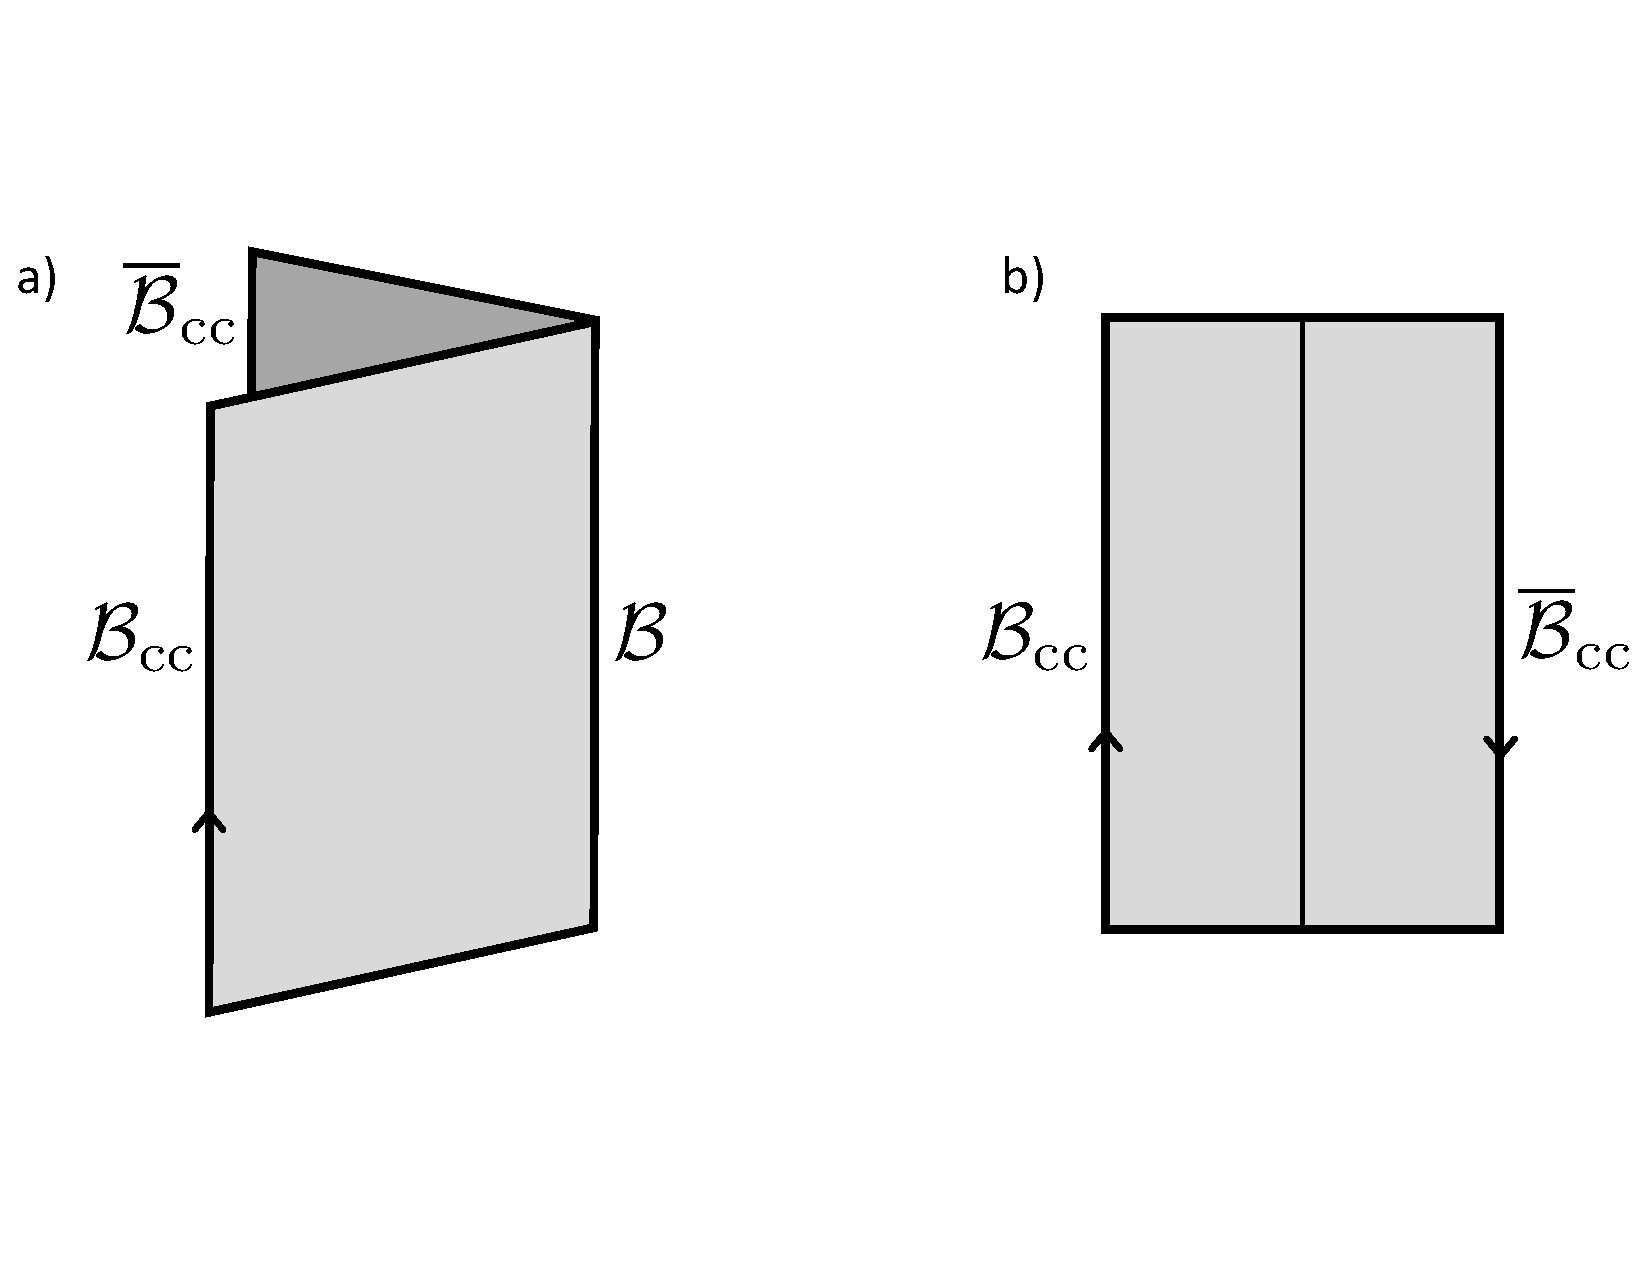
\includegraphics[width=4in]{Folding.pdf}
\end{center}
\caption{\small (a) 在折叠构造中，带状区域上有两份 $\sigma$-模型。除在右边界上由支撑于 $\h Y=Y_1\times Y_2$ 中对角线的膜 $\B$ 把它们粘合起来之外，这两个拷贝是解耦的。$\B$ 的 $\CP$ 丛平凡，因此这种粘合是它唯一的作用。(b) 展开之后，我们得到单个 $\sigma$-模型的拷贝，位于宽度加倍的带状区域上。$\B$ 的痕迹不再存在。\label{folding}}
\end{figure}

不过，这个定义有一个有用的变体。为计算 $\Hom(\B,\h\B_\cc)$，我们研究靶空间为 $\h Y$ 的 $\sigma$-模型，定义在带状区域 $\Sigma$ 上，左边界由 $\h\B_\cc$ 设定边界条件，右边界由 $\B$ 设定，如图 \ref{folding}(a)。$\h Y=Y_1\times Y_2$ 的两个因子在 $\sigma$-模型的体内解耦，因为 $\h Y$ 上的度量是乘积度量；它们在左边界上也解耦，因为膜 $\h\B_\cc=\B_{\cc,1}\times \B_{\cc,2}$ 同样是乘积。因此，在带状区域右边界之外，我们可以把 $\Sigma$ 看作有两叶，一叶映到 $Y_1$，一叶映到 $Y_2$，如图所示。两叶只在右边界上耦合；在那里，由于 $\B$ 支撑在 $Y_1\times Y_2$ 的对角线上，两叶被“粘在一起”，映到 $Y$ 中的同一点。这提示我们应该“展开”这幅图（图 \ref{folding}(b)）。展开之后，我们简单地得到宽度加倍的单叶，它映到 $Y$ 的单个拷贝。展开会反转折叠图中两叶之一的定向，而这种定向反转改变 $A$-模型辛形式的符号。在折叠图中，$A$-模型辛形式在 $Y_1$ 上是 $\frac{1}{2}\omega_K$，在 $Y_2$ 上是 $-\frac{1}{2}\omega_K$；因此展开之后，$A$-模型辛形式处处是 $\frac{1}{2}\omega_K$。换言之，展开图涉及 $Y$ 单个拷贝的通常 $A$-模型，其辛形式为 $\frac{1}{2}\omega_K$。展开之前，膜 $\B_{\cc,1}$ 与 $\B_{\cc,2}$ 的 $\CP$ 丛曲率都是 $\frac{1}{2} \omega_J$。反转 $\Sigma$ 的定向会把膜的 $\CP$ 丛换成其对偶丛（秩 1 情形下即其逆丛），从而反转 $\CP$ 曲率的符号。因此在展开图中，边界由膜 $\B_\cc$ 与 $\bB_\cc$ 标记，它们的 $\CP$ 丛分别是曲率为 $\frac{1}{2}\omega_J$ 与 $-\frac{1}{2}\omega_J$ 的线丛 $\L$ 与 $\L^{-1}$。\zy{原文作“lines bundles”，显系“line bundles”（线丛）之误；译文径改。} 这些就是第 \ref{background} 节引入的共轭典范余迷向膜。预量子线丛仍是 $\frL=\L^2$。$\A=\Hom(\B_\cc,\B_\cc)$ 是 $Y$ 上全纯函数交换代数 $\A_0$ 的形变量子化，$\b\A=\Hom(\bB_\cc,\bB_\cc)$ 类似地是 $Y$ 上反全纯函数代数 $\bA_0$ 的形变量子化。折叠图中的 $\H=\Hom(\B,\h\B_\cc)$，在展开图中变为 $\H=\Hom(\bar\B_\cc,\B_\cc)$。

无论用哪种描述 $\H$，我们都需要在 $\H$ 上定义埃尔米特内积。为确定起见，我们使用折叠的语言。\footnote{关于以下内容的更多细节，见 \cite{GW} 第 2.7 节。} 拓扑场论一般会给出 $\H=\Hom(\B,\h\B_\cc)$ 与其对偶空间 $\H'=\Hom(\h\B_\cc,\B)$ 之间的非退化双线性（而非埃尔米特）配对 $(~,~)$。要在 $\H$ 上得到埃尔米特配对，我们需要把这个双线性配对与一个从 $\H$ 到 $\H'$ 的反线性映射复合。在底层物理理论中，这样的映射由 $\sf{CPT}$ 对称性 $\Theta$ 提供。但 $\Theta$ 不是 $A$-模型对称性；它把 $A$-模型映到辛形式符号相反的共轭 $A$-模型。交换 $\h Y$ 两个因子的对合 $\tau$ 也把 $A$-模型与其共轭互换，因为它是反辛的（它反转 $A$-模型辛形式的符号），所以 $\Theta_\tau=\Theta\tau$ 是 $A$-模型的反线性对称性。最后，由于膜 $\B$ 与 $\B_\cc$ 是 $\Theta_\tau$-不变的，$\Theta_\tau$ 把 $\H$ 映到 $\H'$，于是我们可以通过
\be\label{hermdef}\la \psi,\psi'\ra= (\Theta_\tau\psi,\psi').\ee
在 $\H$ 上定义一个非退化埃尔米特配对。对一般的 $\Theta_\tau$-不变膜，这样的配对不是正定的。对于量子化余切丛这一特殊情形——它是我们在 $A$-模型一侧的主要例子——人们预期正定性成立。这一构造的 $B$-模型类比使用反全纯（而非反辛）对合 $\tau$。此情形下配对的正定性是微妙的，附录 \ref{bmodel} 中有讨论。

在折叠图中，$\tau$（因而 $\Theta_\tau$）交换 $\h Y=Y_1\times Y_2$ 的两个因子；在展开图中，它们交换带状区域的两端。交换带状区域的两端会反转带状区域的定向，从而会改变 $\sB$ 的符号。因此在 $\sB\not=0$ 的描述中，内积的定义不那么自然（需要给 $\Theta_\tau$ 配上一个 $B$-场规范变换）。这就是为什么我们在求解秩 1 余迷向膜的 Kapustin–Orlov 条件时取 $\sB=0$。

% ch03: 原文 GLDraft_D.tex 行 560–732；§2.3–2.4
% 只译散文（标题、正文、图题、脚注）；公式、\label、\ref、\eqref、\cite、图文件名保持不变。

 \subsection{希格斯丛模空间的量子化}\label{aphiggs}
 
 为了把这一构造用于某个规范群 $G$ 与黎曼曲面 $C$ 所对应的 $\M_H(G,C)$ 的量子化，我们真正需要研究的是它的四维版本。这意味着，要在 $\Sigma\times C$ 上研究规范群为 $G$ 的 $\N=4$ 超杨–米尔斯理论，其中 $\Sigma$ 是图 \ref{folding}(b) 中的长条。长条左、右两侧的边界条件，由 $\B_\cc$ 与 $\bB_\cc$ 的规范场论版本给出。$\B_\cc$ 在四维规范场论语言中的详细描述见 \cite{KW} 第 12.4 节。我们可以用一对 $(A,\phi)$ 来描述 $C$ 上的希格斯丛（Higgs bundle），其中 $A$ 是规范场，即 $G$-丛 $E\to C$ 上的一个联络\zy{原文作 $E\to G$，显系笔误——$G$ 是规范群，丛的底空间应是黎曼曲面 $C$；译文径改。}，$\phi$ 是取值于伴随丛（adjoint bundle）$\ad(E)$ 的 1-形式。在这一描述下，$\bB_\cc$ 由 $\B_\cc$ 经 $(A,\phi)\to (A,-\phi)$ 得到（并适当地延拓到四维超多重态的其他分量）。这是希格斯丛模空间上一个熟知的对合：它在复结构 $I$ 下全纯作用，在复结构 $J$ 与 $K$ 下反全纯作用。

尽管我们动用了规范场论与膜的机制，来构造与 $\M_H(G,C)$ 的量子化相联系的希尔伯特空间 $\H$，这一构造的实际产物却完全不令人意外。$\M_H(G,C)$ 中的一个稠密开集是余切丛 $T^*\M(G,C)$，其中 $\M$ 是 $C$ 上半稳定全纯 $G$-丛的模空间。几何量子化——或者干脆说初等量子力学——提示：与 $T^*\M(G,C)$ 的量子化相联系的希尔伯特空间，应当是 $\M(G,C)$ 上 $\lmark^2$ 半密度（half-density）的空间。

之所以要说 $\lmark^2$ 半密度而不说 $\lmark^2$ 函数，是因为在未选定某种测度\footnote{空间 $\M(G,C)$ 其实确有自然的测度，即把它视为 $C$ 上结构群为紧致群 $G$ 的平坦丛的模空间时，由其所携带的实辛结构给出的测度。这也是它嵌入超凯勒流形 $\M_H(G,C)$ 所诱导的测度。然而，这一测度并不属于 $A$-模型，也不会自然地出现在诸如希尔伯特空间 $\H$ 的定义这样的 $A$-模型构造中。}的一般光滑流形 $N$ 上，函数无从积分，因而没有自然的 $\lmark^2$ 函数的希尔伯特空间。流形 $N$ 上的一个密度是平凡实线丛 $\K$ 的一个截面，在任意坐标系中可局部写作 $|\d x^1\d x^2\cdots \d x^w| \,f(x^1,x^2,\cdots, x^w)$，其中 $f(x^1,\cdots, x^w)$ 是函数，而 $|\d x^1\d x^2\cdots \d x^w|$ 是测度，不是微分形式。$\K$ 有平方根 $\K^{1/2}$，它也是平凡的；其截面在给定坐标系中局部由函数 $g(x^1,x^2,\cdots, x^w)$ 描述，这些函数在坐标变换下的变换方式使得 $|\d x^1\d x^2\cdots \d x^w| \,g(x^1,x^2,\cdots, x^w)^2$ 不变。方便起见，把 $\K^{1/2}$ 的截面形式地写作
\be\label{formw} h=|\d x^1\d x^2\cdots \d x^w|^{1/2} g(x^1,x^2,\cdots, x^w)\ee
复值半密度由同一公式描述，只是局部 $g$ 取复值函数；它们以显然的方式构成希尔伯特空间：\be\label{ob} ||h||^2=\int |\d x^1\d x^2\cdots \d x^w|\, |g(x^1,x^2\cdots x^w)|^2.\ee
现在，出于将要应用于复流形 $\M(G,C)$ 的考虑，我们来描述复流形 $N$ 上的密度丛与半密度丛。若 $N$ 的复维数为 $n=w/2$，局部全纯坐标为 $z^1,z^2,\cdots, z^n$，则 $|\d z^1 \d z^2 \cdots \d z^n \d \bar z^1\d\bar z^2\cdots \d\bar z^n|$ 是 $N$ 上的一个密度，换言之是 $\K\to N$ 的一个截面。另一方面，$\d z^1 \d z^2 \cdots \d z^n $ 是全纯典范丛 $K\to N$ 的截面，而 $ \d \bar z^1\d\bar z^2\cdots \d\bar z^n$ 是复共轭线丛 $\bar K\to N$ 的截面（若给 $N$ 赋予相反的复结构，也可把它视为 $N$ 的典范线丛）。于是 $\K$ 可以等同于 $K\otimes \bar K$；更精确地说，$K\otimes \bar K\cong \K\otimes _\R\C$，即 $K\otimes \bar K$ 是复值密度丛 $\K$ 的复化。类似地，$K$ 至少在局部总有平方根；并且对 $K$ 的任一局部平方根的选取，都有 $\K^{1/2}\cong K^{1/2}\otimes \bar K{}^{1/2}$；更精确地说，$K^{1/2}\otimes \bar K^{1/2}\cong \K^{1/2}\otimes_\R \C$，即 $K^{1/2}\otimes \bar K^{1/2}$ 是复值半密度丛。只要 $\bar K{}^{1/2}$ 取作 $K^{1/2}$ 的复共轭，这一关系对 $K^{1/2}$ 的任意选取都成立。

在 \cite{GW} 第 3 节中，作者描述了这样的判别准则：$M=T^*N$ 的膜量子化（brane quantization），在赋予其余切丛的标准辛结构时，会导致 $N$ 上 $\lmark^2$ 半密度的希尔伯特空间。除了要求 $M=T^*N$ 有一个适合膜量子化的复化 $Y$ 之外，必要的条件是：$Y$ 应当是 $N$ 的某个复化 $W$ 的余切丛（并且 $Y$ 应具有余切丛自然的复辛结构）。若 $M$ 与 $N$ 本身已是复流形，而 $Y$ 定义为 $M$ 的两份拷贝之积、两份上赋予相反的复结构，则这一条件自动满足。

希格斯丛模空间 $\M_H(G,C)$ 以 $T^*\M(G,C)$ 为稠密开集，但它实际上并不同构于 $T^*\M(G,C)$。人们不会指望一个测度为零的差异会在 $\lmark^2$ 波函数的希尔伯特空间的定义中起重要作用。\cite{GW} 中的构造把量子化 $\M_H(G,C)$ 所得的希尔伯特空间 $\H$ 映到 $\M(G,C)$ 上的半密度空间，并不要求 $T^*\M(G,C)$ 恰好是整个 $\M_H(G,C)$。

$\M(G,C)$ 上半密度的希尔伯特空间 $\H$，早在 \cite{EFK} 中就已引入，那里完全没有提到膜、$\sigma$-模型或规范场论。通过膜的解释，才有可能运用电–磁对偶以及规范场论的其他方法。下一节讨论 Hitchin 哈密顿量时，我们会看到一个例子。


\subsection{Hitchin 哈密顿量}\label{hh}

如我们所见，在把一个复流形（例如 $\M_H(G,C)$）当作实辛流形来作膜量子化时，希尔伯特空间有一个展开（unfolded）的描述：$\H=\Hom(\bar\B_\cc,\B_\cc)$。$\H$ 承载\footnote{在折叠图像（folded picture）中，我们反而有代数 $\Hom(\B_{\cc,1},\B_{\cc,1})$ 与 $\Hom(\B_{\cc,2},\B_{\cc,2})$ 两者的左作用。一个代数的左作用，等同于其反代数的右作用。（反代数的概念在 \cite{GW} 的附录 C 中作了解释。）展开会逆转图 \ref{folding} 中一张叶片的定向，从而把两个代数之一换成其反代数。当然，哪个代数在左作用、哪个在右作用，取决于某些选取。这些在本文中都不重要，因为 $\A$ 与 $\b\A$ 将是交换的，从而同构于其反代数。} $\A=\Hom(\B_\cc,\B_\cc)$ 的左作用与 $\bar\A=\Hom(\bar\B_\cc,\bar\B_\cc)$ 的右作用。$\A$ 与 $\bar\A$ 分别是 $Y$ 上全纯函数所成交换环 $\A_0$ 与 $\bar\A_0$ 的量子形变。一般而言，形变所得的代数可以是非交换的；但在 $\M_H(G,C)$ 这一特殊情形中，$\A$ 与 $\bar\A$ 恰是交换的，因而左作用与右作用没有区别。


具体地说，在复结构 $I$ 下，$\M_H(G,C)$ 上全纯函数之环 $\A_0$ 就是 Hitchin 纤维化（Hitchin fibration）底空间上的函数环 \cite{H,NH}。考虑 Hitchin 方程的一个解 $(A,\phi)$，其中 $A$ 是 $G$-丛 $E\to C$ 上的联络，$\phi$ 是取值于 $\ad(E)$ 的 $1$-形式。令 $\varphi$ 为全纯希格斯场，即 $\phi$ 的 $(1,0)$ 部分。Hitchin 方程给出 $\bar\partial_A\varphi=0$。于是，若 $\P$ 是 $G_\C$ 的李代数 ${\g}_\C$ 上某个次数为 $s$ 的齐次不变多项式（invariant polynomial），则 $\P(\varphi)$ 是 $K_C^s$ 的全纯截面（$K_C$ 为 $C$ 的典范丛；我们还将记 $T_C=K_C^{-1}$）。给定 $C$ 上任一取值于 $T_C^{s-1}$ 的 $(0,1)$-形式 $\alpha$，可以定义
\be\label{juno} H_{\P,\alpha}=\int_C \alpha \,\P(\varphi). \ee
这是 $\M_H$ 上的全纯函数，且只依赖于 $\alpha$ 在 $H^1(C,T_C^{s-1})$ 中的上同调类。$H^1(C,T_C^{s-1})$ 的维数为 $(s+1)(g-1)$，这正是给定 $\P$ 时线性无关函数 $H_{\P,\alpha}$ 的个数。对 $G=\SU(2)$，$\M_H(G,C)$ 上全纯函数之环 $\A_0$ 由 $\P(\varphi)=\Tr\,\varphi^2$ 所对应的那些 $H_{\P,\alpha}$ 生成。更一般地，秩为 $r$ 的单李群 $G$ 有 $r$ 个独立的 Casimir 算子，对应 $r$ 个次数各异的齐次多项式 $\P_j$，$j=1,\cdots,r$，而 $\A_0$ 由 $H_{\P_j,\alpha_j}$ 生成。例如，若 $G=\SU(N)$，可取生成多项式为 $\Tr\,\varphi^{k}$，$k=2,3,\cdots,N$。

函数 $H_{\P_j,\alpha_j}$ 两两 泊松交换，因为 $\M_H(G,C)$ 在复结构 $I$ 下的全纯辛结构使得 $\varphi_z$ 与 $A_{\bar z}$ 成为共轭变量，特别地，任何只由 $\varphi$（而不含 $A$）构造的函数都两两 泊松交换。这些 泊松交换的函数就是 Hitchin 经典可积系统的哈密顿量。

\begin{yizhu}[译者按：Hitchin 纤维化与经典可积系统]
$\M_H$ 在复结构 $I$ 下是复辛流形，复维数为 $2\dim G\,(g-1)$；Hitchin 纤维化 $\M_H\to B$ 把希格斯丛映到其希格斯场的特征多项式（等价地，各次不变多项式 $\P_j(\varphi)$ 的取值），底空间 $B$ 是仿射空间 $\bigoplus_{j}H^0(C,K_C^{d_j})$，其中 $d_j$ 为 $G$ 各 Casimir 算子的次数，$\dim B=\dim G\,(g-1)$。原文说 $\A_0$ 是底空间上的函数环，意即 $\M_H$ 的整体全纯函数都来自底空间；这些 $H_{\P_j,\alpha_j}$ 两两 泊松交换，给出一个完全可积系统。对 $G=\SU(N)$，$B=\bigoplus_{s=2}^{N}H^0(C,K_C^{s})$，$\dim B=(N^2-1)(g-1)$。参见 Hitchin, ``The self-duality equations on a Riemann surface,'' Proc. London Math. Soc. {\bf 55} (1987) 59--126（即 \cite{H}），以及 ``Stable bundles and integrable systems,'' Duke Math. J. {\bf 54} (1987)（即 \cite{NH}）；亦见 \cite{BD}。
\end{yizhu}

从 $\A_0$ 到 $\A$ 的量子形变是无障碍的，意思是 $\A_0$ 的每个元素都可以量子形变到 $\A$ 的一个元素。具体地说，这句话意味着：若 $\P$ 是 $\g$ 上某个次数为 $s$ 的齐次不变多项式，$H_{\P,\alpha}$ 是对应的 Hitchin 哈密顿量，则存在一个微分算子 $D_{\P,\alpha}$，它作用在 $K^{1/2}\to \M(G,C)$ 的截面上，其主象征（leading symbol）等于 $H_{\P,\alpha}$。\zy{译者按（无外部依据）：$s$ 阶微分算子的主象征是其最高阶部分在余切丛上对应的函数，沿纤维为 $s$ 次齐次；对作用在半密度上的算子，它正是 $T^*\M(G,C)$ 上的函数，故可与 $H_{\P,\alpha}$ 相比较。}从 $H_{\P,\alpha}$ 到 $D_{\P,\alpha}$ 的过渡并不完全典范，因为指定 $D_{\P,\alpha}$ 所需的主象征之后，仍可给 $D_{\P,\alpha}$ 加上一个整体定义的低次全纯微分算子（次数小于 $s$）。对 $G_\C=\SL(2,\C)$，可取 $\P$ 的次数为 2，此时唯一整体定义的低次全纯微分算子就是 0 次算子——复常数。对秩更高的群，一般还有更多可能。在数学上，形变无障碍这一事实来自：对任何单群 $G$，$H^1(\M_H,\O)=0$，因此形变中没有潜在的障碍。这一论证的规范场论版本见附录 \ref{coho}，它细化了 \cite{KW} 中先前的讨论。

从 $\sigma$-模型或底层规范场论的角度看，从 $H_{\P,\alpha}$ 到 $D_{\P,\alpha}$ 的形变来自按 $\hbar$ 的幂次展开。这一展开在有限步之后终止，因为我们定义 $\A_0$ 由这样的函数组成：它们在余切丛的纤维上的限制是多项式。$\sigma$-模型或规范场论的具体定义给出从 $H_{\P,\alpha}$ 过渡到 $D_{\P,\alpha}$ 的具体处方，但这依赖于 $A$-模型并不包含的数据（例如 $C$ 上的黎曼度规，而不只是复结构）。

 \begin{figure}
 \begin{center}
   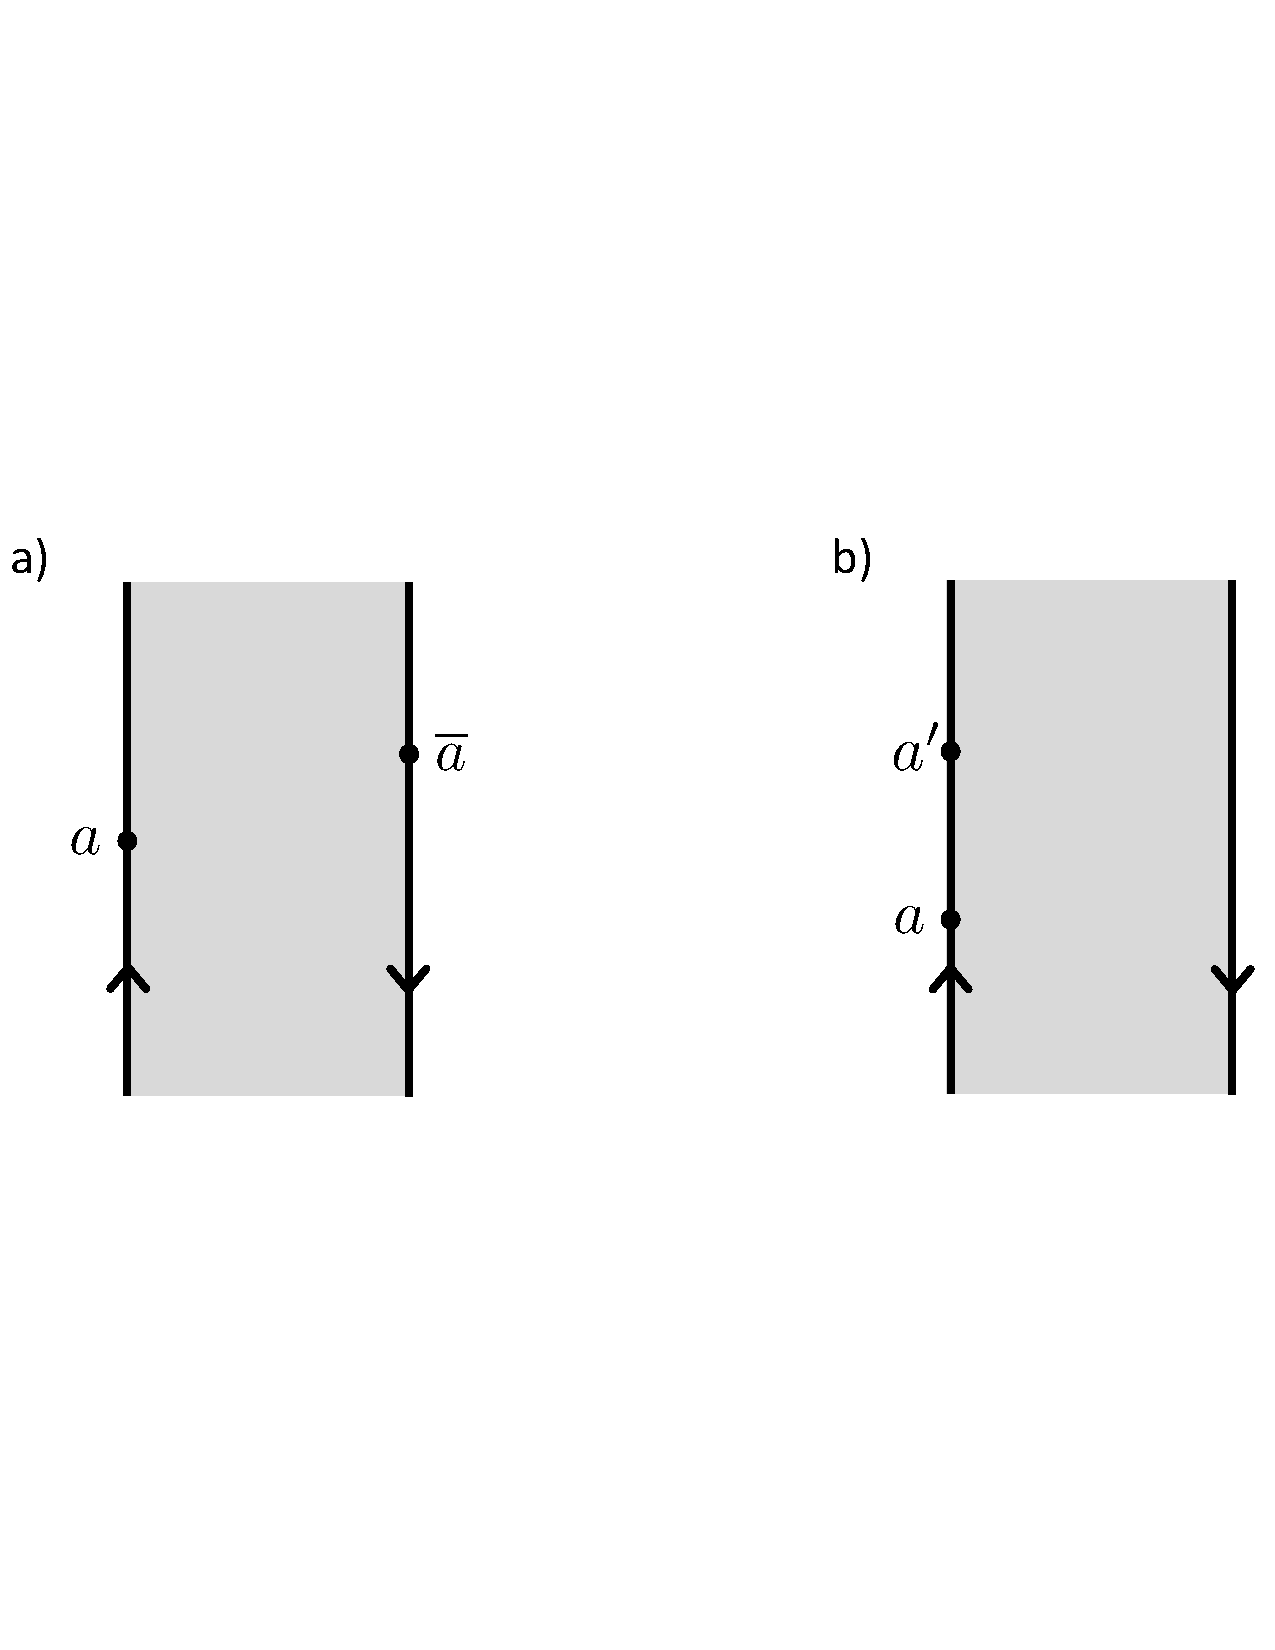
\includegraphics[width=4in]{Timing.pdf}
 \end{center}
\caption{\small (a) 作为二维拓扑场论中的一般性陈述，$\A=\Hom(\B_\cc,\B_\cc)$ 与 $\b\A=\Hom(\b\B_\cc,\b\B_\cc)$ 在作用于 $\H=\Hom(\b\B_\cc,\B_\cc)$ 时彼此交换，因为元素 $a\in\A$ 与 $\b a\in \b\A$ 被插入到相对的边界上。微分同胚不变性不允许任何关于谁“先”被插入的自然概念。(b) 一般而言，在二维拓扑场论中，$\A$（以及类似地 $\b\A$）可以是非交换的，因为元素 $a,a'\in\A$ 以相对于边界定向的确定次序被插入同一边界上。然而，在当前语境中还有两个额外的维度，即黎曼曲面 $C$，它们没有画在二维图像中。可以假定 $a$ 与 $a'$ 在 $C$ 中具有不相交的支集。因此，它们可以彼此上下错动而不出现奇点，故必须交换。\label{sliding}}
 \end{figure} 
 
接下来我们要解释为什么 $\A$ 像 $\A_0$ 一样是交换的。这最初由 Hitchin \cite{H2} 对 $\SU(2)$ 证明，并由 Beilinson 与 Drinfeld \cite{BD} 对一般单群 $G$ 证明。我们将给出一个类似于 \cite{KW} 中的四维解释。当然，同样的考虑也适用于 $\bar\A$。作为热身，先解释为什么 $\A$ 与 $\b\A$ 交换。这一点从以下事实即可看出（图 \ref{sliding}(a)）：元素 $a\in \A$ 插入在长条的左边界，而元素 $\bar a\in \b\A$ 插入在右边界。在二维拓扑场论中，我们可以沿边界独立地把这些插入上下滑动。两个边界插入之间没有有意义的相对时间序，因此它们必须交换。相比之下，考虑一对元素 $a,a'\in\A$ 的插入（图 \ref{sliding}(b)）。此时，作为二维拓扑场论中的一般性陈述，$a$ 与 $a'$ 之间存在有意义的时间序。若试图让其中之一在时间上滑过另一个，它们在交叉时可能出现不连续，因此一般而言可能有 $aa'\not=a'a$。然而，在当前问题中，我们其实不在二维而在四维；还有两个额外的维度构成黎曼曲面 $C$，它们未在图中画出。式 (\ref{juno}) 中 $H_{\P,\alpha}$ 的定义只依赖于 $\alpha$ 在 $H^1(C,T_C^{s-1})$ 中的上同调类。我们可以选取一个支集位于 $C$ 中任意选定的小开球内的代表元。因此，当我们考虑一对元素 $a,a'\in \A$ 时，可以假定它们由在 $C$ 中支集不相交的算子表示。于是，在图 \ref{sliding}(b) 的二维图像中，我们可以把这两个算子彼此上下错动而不出现任何奇点。因此它们交换。\zy{译者按：图内标题 “Diffemorphism inariance” 当为 “Diffeomorphism invariance” 之误（微分同胚不变性）。此系原文文字校勘，无外部依据；译文已按正名译出。}

我们可以稍加阐述量子 Hitchin 哈密顿量的四维起源。经典 Hitchin 哈密顿量中的被积函数 $\P(\varphi)$ 全纯地依赖于 $C$。正如我们在第 \ref{sec:chiral} 节所回顾的，量子 Hitchin 哈密顿量 $D_{\P,\alpha}$ 也可以写成 \be\label{qjuno} D_{\P,\alpha}=\int_C \alpha \,{\cal D}_{\P} \ee
其中 ${\cal D}_{\P}$ 是某些微分算子，它们在点 $p\in C$ 处局部地作用于丛上，并全纯地依赖于 $p$。我们把 ${\cal D}_{\P}(p)$ 认定为某个四维边界局部算符 $O_{\P}(p)$ 的作用。边界条件的全纯-拓扑（holomorphic–topological）性质保证：这类边界局部算符在拓扑方向上彼此交换，并且彼此之间的算子乘积展开（OPE）是非奇异的。

正如第 \ref{aphiggs} 节所解释的，量子希尔伯特空间 $\H=\Hom(\b\B_\cc,\B_\cc)$ 是 $\M(G,C)$ 上 $\lmark^2$ 半密度的空间，等价地，是 $K^{1/2}\otimes \bar K{}^{1/2}$ 的 $\lmark^2$ 截面的空间。我们回忆，之所以如此，是因为 $\M_H(G,C)$ 的膜量子化等价于把它作为余切丛 $T^*\M(G,C)$ 来量子化。在量子化余切丛 $T^*W$ 时，一个在余切丛纤维上的限制为 $s$ 次多项式的函数，会变成作用在 $W$ 上半密度上的 $s$ 次微分算子。若如当前所关心的情形那样 $W$ 是复流形，则更具体地说，$T^*W$ 上的全纯函数变成 $W$ 上的全纯微分算子。从全纯的观点看，人们通常说：$T^*W$ 上的全纯函数（对纤维为多项式依赖）变成作用在 $K^{1/2}$ 的截面上的全纯微分算子。（$K^{1/2}$ 的作用在 \cite{GW} 第 3.2 节与附录 C 中从 $\sigma$-模型的观点作了解释。）就 Hitchin 哈密顿量而言，它们可以被量子形变为作用在 $K^{1/2}$ 的截面上、而非任何其他全纯线丛的截面上的微分算子，这属于标准叙述的一部分 \cite{H2,BD}。然而，反全纯线丛 $\bar K{}^{1/2}$ 对于全纯微分算子是不可见的，因为它的转移函数是反全纯的，与全纯微分算子交换。因此，由 $T^*W$ 上全纯函数的形变量子化所得的全纯微分算子，自然地可以作用在 $K^{1/2}\otimes \bar K{}^{1/2}$ 上，等价地，作用在半密度丛 $\K^{1/2}$ 上。类似地，在形变量子化之下，$T^*W$ 上的反全纯函数变成作用在 $\K^{1/2}$ 上的反全纯微分算子。




 

于是 $\A$ 与 $\bA$ 分别成为作用在 $\M(G,C)$ 上半密度上的全纯与反全纯微分算子代数。从这个观点看，$\A$ 与 $\bA$ 交换这一陈述不过反映了全纯微分算子与反全纯微分算子交换这一事实。

% ch04: 原文 GLDraft_D.tex 行 733–1033；§2.5–2.8
% 只译散文（标题、正文、图题、脚注）；公式、\label、\ref、\eqref、\cite、图文件名保持不变。

\subsection{余迷向膜的对偶}\label{dualco}

为了能把对偶性用于这个问题，我们还需要一个要素：需要理解 $B$-模型（所在空间为 $\M_H(G^\vee,C)$）中 $A$-膜 $\B_\cc$ 与 $\bB_\cc$ 的对偶对象。确切地说，这里指的是 \cite{H} 中称为 $J$ 的复结构下的 $B$-模型；在此复结构下，$\M_H(G^\vee,C)$ 参数化 $C$ 上结构群为 $G^\vee_\C$ 的平坦丛。我们把平坦丛上的联络记作 $\cA=A+\i\phi$，其中 $(A,\phi)$ 是 Hitchin 方程中出现的酉联络与希格斯场。一般的 $B$-膜是 $\M_H(G^\vee,C)$ 上的凝聚层（coherent sheaf），或凝聚层的复形。然而，$A$-膜 $\B_\cc$ 与 $\bB_\cc$ 具有一些额外性质，这些性质意味着它们的对偶 $B$-膜必定相当特殊。

为解释这一点，我们回顾：希格斯丛模空间是超凯勒（hyperkähler）流形，具有复结构 $I,J,K$，它们满足通常的四元数关系，并配有相应的凯勒形式 $\omega_I,\omega_J,\omega_K$ 与复辛形式 $\Omega_I=\omega_J+\i \omega_K$ 等等。几何朗兰兹对偶一般把带有辛结构 $\omega_K$ 的 $\M_H(G,C)$ 的 $A$-模型，映为复结构 $J$ 下 $\M_H(G^\vee,C)$ 的 $B$-模型。当我们不加说明地谈论 $A$-模型或 $B$-模型时，指的就是这两个模型。

在这两个模型中，一般的膜只不过是适当类型的 $A$-膜或 $B$-膜。然而，几何朗兰兹中许多最重要的膜还具有额外性质。例如，支撑在 $\M_H(G^\vee,C)$ 中一点上的膜是类型 $(B,B,B)$ 的膜，也就是说，它在复结构 $I,J$ 与 $K$（或它们的任意线性组合）下都是 $B$-膜。类型 $(B,B,B)$ 的膜的对偶是类型 $(B,A,A)$ 的膜；在希格斯丛模空间的情形，支撑在一点上的秩 1 膜的对偶，是支撑在 Hitchin 纤维化的一条纤维上、带有秩 1 平坦 $\CP$ 丛的膜。这些膜就是 Hecke 本征层，它们是几何朗兰兹纲领研究的中心对象，将在第 \ref{wkb} 节讨论。就当前情形而言，$\B_\cc$ 与 $\bB_\cc$ 是类型 $(A,B,A)$ 的膜：凭借 Kapustin–Orlov 关于余迷向膜（coisotropic brane）的条件，它们是类型 $I$ 与 $K$ 的 $A$-膜；又因为其 $\CP$ 丛的曲率 $\pm\frac{1}{2}\omega_J$ 在复结构 $J$ 下为 $(1,1)$ 型，所以这些丛在复结构 $J$ 下全纯，从而是类型 $J$ 的 $B$-膜。一般地，类型 $(A,B,A)$ 的膜的对偶仍是类型 $(A,B,A)$ 的膜，因此 $\B_\cc$ 与 $\bB_\cc$ 的对偶将是这种类型的膜。类型 $(A,B,A)$ 的膜中最简单的一类，由复结构 $J$ 下某个复拉格朗日子流形（complex Lagrangian submanifold）的结构层给出；用更物理的语言说，这些是支撑在复拉格朗日子流形上、带有平凡 $\CP$ 丛的膜。确实，$\B_\cc$ 与 $\bB_\cc$ 的对偶正是这种类型。这些对偶最早由 Beilinson 与 Drinfeld \cite{BD}（用一种不同的表述）识别出来，其依据是临界 level $k=-h^\vee$ 的共形场论；规范场论的解释则涉及弦论中 D3–NS5 系统与 D3–D5 系统之间的对偶 \cite{GWknots}。\zy{$A$-膜并不一定支撑在拉格朗日子流形上：Kapustin 与 Orlov 指出，支撑在余迷向子流形上、并带有适当 $\CP$ 丛的膜也可以是 $A$-膜，其曲率须满足与辛形式相容的方程。参见 \cite{KO}；在几何朗兰兹语境中的讨论见 \cite{KW}。}

支撑 $\B_\cc$ 的对偶的复拉格朗日子流形，参数化满足“全纯 oper”条件的平坦 $G^\vee_C$ 丛，我们把它记作 $L_\op$。类似地，$\bB_\cc$ 的对偶支撑在复拉格朗日子流形 $L_\bop$ 上，后者参数化满足“反全纯 oper”条件的平坦 $G^\vee_C$ 丛。

全纯 oper 条件可以相当简洁地表述为对丛的全纯类型、即对 $\cA$ 的 $(0,1)$ 部分的整体约束，本文即采用这种表述；它也可以像第 \ref{localoper} 节那样用更局部的方式表述。这两种表述在数学上都是标准的。在四维规范场论中，$S$-对偶把变形 Neumann 边界条件映为变形的“Nahm 极点”边界条件，后者直接给出局部约束 \cite{GWknots}。

定义 $\M_H(G^\vee,C)$ 的复拉格朗日子流形的一种一般方式，是考虑所有具有某个固定全纯类型的平坦 $G^\vee_C$ 丛 $E^\vee\to C$。指定丛的全纯类型，等价于指定 $\cA$ 的 $(0,1)$ 部分。这里以及下面马上要考虑的几个类似情形中，除要求完整联络平坦之外，我们对联络的 $(1,0)$ 部分不加任何约束。在保持 $E^\vee$ 上联络平坦的前提下，我们可以给联络的 $(1,0)$ 部分加上任意的 $\bar\partial_\cA$-闭形式，它代表 $H^0(C,K_C\otimes \ad(E^\vee))$ 中的一个元素。这个空间的维数是 $\M_H(G^\vee,C)$ 维数的一半，所以具有指定全纯类型的平坦 $G^\vee_\C$ 丛构成 $\M_H(G^\vee,C)$ 的一个中间维数子流形 $L$。$L$ 是复拉格朗日子流形，因为复结构 $J$ 下 $\M_H(G^\vee,C)$ 的全纯辛结构 $\Omega_J$ 是 $\cA$ 的 $(1,0)$ 部分与 $(0,1)$ 部分之间的配对，一旦指定 $(0,1)$ 部分便为零。一旦在 $L$ 中选定一个基点，$L$ 就同构于向量空间 $H^0(C,K_C\otimes \ad(E^\vee))$。

我们可以在 $\M_H(G^\vee,C)$ 的同一复结构下定义第二族复拉格朗日子流形：指定平坦 $G^\vee_\C$ 丛的反全纯结构。这相当于指定 $\cA$ 的 $(1,0)$ 部分而让 $(0,1)$ 部分变化；出于与前面相同的理由，它给出一个复拉格朗日子流形。固定 $\cA$ 的 $(1,0)$ 部分或 $(0,1)$ 部分竟然是复结构 $J$ 下的全纯条件，这也许稍感意外。确实，希格斯丛模空间上的复结构 $J$ 对二维流形 $C$ 的复结构并不敏感，它把 $\cA$ 的 $(1,0)$ 部分与 $(0,1)$ 部分完全对称地对待。

子流形 $L_\op$ 与 $L_\bop$ 可以通过指定平坦 $E^\vee$ 丛的全纯结构或反全纯结构的一种特定选择来定义。先解释 $G_\C=\SL(2,\C)$ 情形的定义。对这个群，一个 oper 是平坦丛 $E^\vee\to C$，它作为全纯丛是 $K_C^{-1/2}$ 被 $K_C^{1/2}$ 的非平凡扩张：
\be\label{nonex}0\to K_C^{1/2}\to E^\vee\to K_C^{-1/2}\to 0. \ee
这样的非平凡扩张在同构意义下唯一。因此，这一全纯类型的平坦丛族构成一个复拉格朗日子流形，我们称它为 $L_\op$。作此定义时，我们选定了 $K_C^{1/2}$，等价地选定了 $C$ 上的一个旋量结构（spin structure）。确实，对 $\SL(2,\C)$ 而言，oper 的定义依赖于这样的旋量结构选择（尽管我们在 $L_\op$ 的记号中不体现这一点）。我们将在第 \ref{toposubt} 节回到这一点。

一旦选定基点，即选定一个具有 oper 类型、带平坦联络 $\cA_0$ 的特定 $\SL(2,\C)$ 丛 $E^\vee$，就可以对 $L_\op$ 给出简单的描述。在把 $E^\vee$ 作为 oper 变形时，我们不妨保持 $\cA_0$ 的 $(0,1)$ 部分不变，因为只要求在复规范变换的意义下保持它不变。但我们可以修改 $\cA_0$ 的 $(1,0)$ 部分。为在保持 $\cA_0$ 平坦的同时作此修改，我们给 $\cA_0$ 加上一个 $\bar\partial_{\cA_0}$-闭的 $(1,0)$-形式，即 $H^0(C,K_C\otimes \ad(E^\vee))$ 中的一个元素。利用正合列 (\ref{nonex})，可以证明 $H^0(C,K_C\otimes \ad(E^\vee))$ 同构于 $C$ 上二次微分构成的空间。这正是 $\SL(2,\C)$ 的 Hitchin 纤维化的底空间，所以 $L_\op$ 同构于 Hitchin 纤维化的底空间。这一同构并非完全典范，因为它依赖于 $L_\op$ 中基点的选取。类似的推理适用于其他群。

类似地，对 $G_\C=\SL(2,\C)$，反全纯 oper（简称反 oper）是平坦丛 $E^\vee$，它作为反全纯丛是 $\bar K_C^{-1/2}$ 被 $\bar K_C^{1/2}$ 的非平凡扩张：
\be\label{onex} 0\to\bar K_C^{1/2}\to E^\vee \to \bar K_C^{-1/2}\to 0. \ee
这类平坦丛构成的族是另一个复拉格朗日子流形，我们称它为 $L_\bop$。它非典范地同构于 Hitchin 纤维化的底空间，但带有相反的复结构。

一般地，若 $G_\C^\vee$ 是单复 Lie 群，则有 Lie 代数“主嵌入”（principal embedding）${\su}(2)\to {\g^\vee}$ 的概念。例如，若 $G^\vee=\SL(n,\C)$，主嵌入使得 $\g^\vee$ 的 $n$ 维表示在 $\su(2)$ 下不可约地变换；相应的主子群是 $\SL(2,\C)$ 或 $\SO(3,\C)$ 的拷贝，取决于 $n$ 为偶数还是奇数。为简洁起见，我们有时忽略这一微妙之处，直接说主 $\SL(2,\C)$ 子群，尽管群的整体形式有时是 $\SO(3,\C)$。

$G_\C^\vee$ 的 oper 是一个平坦 $G_\C^\vee$ 丛 $E_\C^\vee$，它作为全纯丛等价于某个 $\SL(2,\C)$ oper 丛的主嵌入；也就是说，等价于一个秩二丛的主嵌入，而该秩二丛是形如 (\ref{nonex}) 的非平凡扩张。对 $G^\vee_\C=\SL(n,\C)$，这意味着 oper 丛在全纯意义下是这样的非平凡扩张的 $(n-1)$ 次对称张量幂，因而有一个同构于 $K_C^{(n-1)/2}$ 的子丛：
\be\label{nex}0\to K_C^{(n-1)/2}\to E^\vee\to \cdots \ee
（并带有由 $K_C$ 的幂给出的滤过）。同样，$E_\C^\vee$ 上联络的 $(1,0)$ 部分除要求完整联络平坦之外不受限制。类似地，反全纯 $G_\C^\vee$ oper 是一个平坦 $G_\C^\vee$ 丛，它作为反全纯丛等价于某个反全纯 $\SL(2,\C)$ oper 丛的主嵌入。

在 $\sigma$-模型层面，$\B_\cc$ 与 $\bB_\cc$ 的对偶是 $L_\op$ 与 $L_\bop$ 的结构层；也就是说，它们是分别支撑在 $L_\op$ 与 $L_\bop$ 上、带有平凡 $\CP$ 丛的秩 1 膜 $\B_\op$ 与 $\B_\bop$。

\subsection{局部约束}\label{localoper}

为给出 oper 的更局部的刻画，我们先考虑 $G^\vee_\C=\SL(2,\C)$ 的情形。$E^\vee$ 的扩张结构意味着存在 $E^\vee \otimes K_C^{-1/2}$ 的一个整体全纯截面 $s$。把联络的 $(1,0)$ 部分记作 $D$。$\SL(2,\C)$-不变的组合 $s \wedge D s$ 是 $C$ 上的整体全纯函数。这个函数必定非零：若它为零，我们就可以写 $D s= a s$，而 $a$ 将定义 $K_C^{-1/2}$ 上的一个全纯平坦联络，这样的联络并不存在（对亏格大于 1 的 $C$，或在低亏格但带有抛物结构的情形）。

不失一般性，我们可以归一化 $s$，使 $s \wedge D s=1$。这使 $s$ 在相差一个符号的意义下确定。对 $G^\vee_\C=\SL(2,\C)$，全纯 oper 条件的局部版本正是：$E^\vee \otimes K_C^{-1/2}$ 具有一个整体定义的全纯截面，使得 $s \wedge D s=1$。

求导可得 $s \wedge D^2 s =0$，因此 $s$ 满足二阶微分方程
\begin{equation}\label{stresst}
D^2 s + t s=0
\end{equation}
其中 $t$ 是 $C$ 上的某个“经典应力张量”（classical stress tensor）。在 $C$ 上作局部坐标变换时，$t$ 按应力张量而非二次微分的方式变换。绝非巧合的是，方程 (\ref{stresst}) 可以看作二维共形场论中退化场关联函数的 Belavin–Polyakov–Zamolodchikov（BPZ）微分方程的经典极限。\zy{BPZ 方程是 Belavin、Polyakov 与 Zamolodchikov 在二维共形场论中导出的线性微分方程，来自退化场的零矢量条件；方程 (\ref{stresst}) 是它在经典极限下的形式。参见 A. Belavin, A. Polyakov and A. Zamolodchikov, ``Infinite conformal symmetry in two-dimensional quantum field theory,'' \emph{Nucl. Phys.} B241 (1984) 333。} 经典应力张量可用来定义 oper 流形上全纯函数代数的一组生成元，这些函数形如
\be\label{opjuno2} f_{t,\alpha}=\int_C \alpha \,t ,\ee
其中 $\alpha$ 是取值于 $T_C$ 的 $(0,1)$-形式。

\begin{yizhu}[译者按：经典应力张量]
原文特别指出 $t$ 按应力张量而非二次微分的方式变换，这一区别值得说明。二次微分 $\alpha$ 在局部坐标变换 $z\mapsto w$ 下按 $\alpha\mapsto \alpha\,(dz/dw)^2$ 变换，只含雅可比因子；而应力张量的变换律还含有一项与坐标变换的 Schwarz 导数有关的贡献。因此 $t$ 并不整体地是一个二次微分，而应理解为 $C$ 上的射影联络；在已固定 $K_C^{1/2}$ 的前提下，对 $\SL(2,\C)$，oper 正对应于 $C$ 上的射影结构（参见 \cite{BD}）。这也解释了为什么方程 (\ref{stresst}) 具有共形场论中应力张量方程的形式。
\end{yizhu}

$G^\vee_\C=\SL(n,\C)$ 的情形可以类似地分析。此时 $E^\vee$ 的 oper 结构（方程 (\ref{nex})）意味着存在 $E^\vee \otimes K_C^{(1-n)/2}$ 的一个整体全纯截面 $s$。于是 $s \wedge D s \wedge \cdots D^{n-1} s$ 是 $C$ 上的整体全纯函数，它不能为零，理由与我们对 $n=2$ 所解释的类似。我们可以归一化 $s$，使 $s \wedge D s \wedge \cdots D^{n-1} s=1$；这唯一地确定 $s$，至多相差乘以一个 $n$ 次单位根。由于 $0=D(s \wedge D s \wedge \cdots D^{n-1} s)=s\wedge Ds \wedge \cdots \wedge  D^{n-2}s\wedge D^ns$，可知 $s$ 满足 $n$ 阶微分方程
\begin{equation}
D^n s + t_2 D^{n-2} s+  \cdots + t_n s =0.
\end{equation}
我们可以定义 oper 流形上全纯函数代数的一组生成元，这些函数形如
\be\label{opjunon} f_{t_k,\alpha}=\int_C \alpha \,t_k \ee
其中 $\alpha$ 是取值于 $T_C^{k-1}$ 的 $(0,1)$-形式，$k=2,\cdots,n$。

对一般的 $G^\vee_\C$，没有像 $\SL(n,\C)$ 的 $n$ 维表示那样方便的、可供使用的特殊表示。不过，给定 oper 丛 $E^\vee$，我们可以考虑它在 $G^\vee_\C$ 的任一不可约表示 $R$ 中的伴丛 $E^\vee_R$。按 oper 的定义，$E^\vee_R$ 作为全纯丛的结构群约化到一个秩 1 子群 $H_\C\subset G^\vee_\C$；这个子群同构于 $\SL(2,\C)$ 或 $\SO(3,\C)$，取决于 $G^\vee_\C$ 与 $R$。设 $R_n$ 是 $H_\C$ 的 $n$ 维不可约表示（对 $\SL(2,\C)$，$n$ 为任意正整数；对 $\SO(3,\C)$，$n$ 为任意正奇数）。作为 $H_\C$ 的表示，有 $R\cong \oplus_{n=0}^\infty Q_n\otimes R_n$，其中 $Q_n$ 是某些向量空间，除有限个外均为零。实际上，若 $N$ 是使 $Q_n$ 非零的最大整数，则 $Q_N$ 是一维的，我们可以把 $Q_N\otimes R_N$ 换成 $R_N$。于是 $R\cong R_N\oplus_{n=0}^{N-1}Q_n\otimes R_n$。在这个分解中，$R_N$ 关于 $H$ 的 Borel 子群 $B_H$ 的最高权向量，也是 $G^\vee$ 关于 $G^\vee$ 的、包含 $B_H$ 的 Borel 子群 $B_{G^\vee}$ 的最高权向量。伴丛 $E^\vee_R$ 作为全纯丛有类似的分解
\be\label{regasso} E^\vee_{R}= E^\vee_{R,N}\oplus \left(\oplus_{n=1}^{N-1} Q_n\otimes E^\vee_{R_n}\right),  \ee
其中 $E^\vee_{R_n}$ 是与某个 $H_\C$ oper 在 $n$ 维表示下相伴的全纯丛。对每个 $n$，由方程 (\ref{nex}) 可以得到向量空间 $Q_n$ 到 $E^\vee_{R} \otimes K_C^{(1-n)/2}$ 的整体全纯截面空间中的典范像 $s_{R,n}$；等价地，得到全纯映射
\be\label{holmap} s_{R,n}: Q_n \otimes K_C^{(n-1)/2} \to E^\vee_{R}. \ee

这里特别重要的是“最高权”对象 $s_{R,N}$，我们直接把它记作 $s_R$：
\be\label{linmap}s_R:K_C^{(N-1)/2}\to E^\vee_R. \ee
这里 $N$ 的定义是：表示 $R$ 的最高权向量（相对于某个 Borel 子群 $B$）位于主 $\SL(2,\C)$ 子群的一个 $N$ 维表示中，而该子群的 Borel 子群包含于 $B$ 中。对 $G^\vee=\SL(n,\C)$ 及 $R$ 为 $n$ 维表示或其对偶的情形，$N=n$。

与 $s \wedge D s=1$ 条件部分相似的条件是：对 $m< n\leq N$，截面族 $D^m s_{R,n}$ 应在 $C$ 的每一点张成 $E^\vee_{R}$。于是 $D^n s_{R,n}$ 可以用 $m<n$ 的 $D^m s_{R,n}$ 展开，从而产生一组复杂的微分方程（例子见附录 \ref{somex}）。这些微分方程的系数是 oper 流形上的全纯函数，可以表示为一族可观测量 $T_{\cal P}$ 的导数的多项式，而这些可观测量所用的标签，与 $G^\vee_\C$ 的量子 Hitchin 哈密顿量的被积函数所用的标签相同。形如 $D^m s_{R,n} \otimes D^{m'} s_{R',n'}$ 的张量积，也可以在张量积 $R \otimes R'$ 分解中出现的所有 $R''$ 所对应的 $D^{m''} s_{R'',n''}$ 的基上展开。展开式的系数同样是 oper 流形上的全纯函数，并可表示为一族可观测量 $T_{\cal P}$ 的导数的多项式。

这族可观测量 $T_{\cal P}$ 有时称为 $G^\vee_\C$ 的经典 $W$-代数（classical $W$-algebra）。用这种语言说，$s_{R,n}$ 所满足的微分方程是 BPZ 方程的经典类比，而张量积展开则类似于退化场的算子乘积展开（OPE）。\zy{经典 $W$-代数由 Drinfeld 与 Sokolov 在研究 KdV 型方程时引入；本文所说的经典 $W$-代数即由这族可观测量 $T_{\cal P}$ 生成。参见 V. Drinfeld and V. Sokolov, ``Lie algebras and equations of Korteweg–de Vries type,'' \emph{J. Soviet Math.} 30 (1985)。}

在四维规范场论中，变形 Neumann 边界条件与变形的 Nahm 极点边界条件互为 $S$-对偶，后者也是全纯-拓扑（holomorphic–topological）的。这个边界条件涉及规范场在边界处某种指定的奇异性。实际上，物理理论中这些奇异的边界条件，在拓扑扭化后的理论中给出一个 oper 边界条件。场在次主导行为中所含的规范不变信息，由边界局部算符承载；这些算符与 $T_{\cal P}$ 可观测量相匹配，并与变形 Neumann 边界条件处用于定义量子 Hitchin 哈密顿量的相应局部算符 $S$-对偶。\footnote{oper 边界条件处的局部算符还包括 oper 流形上的全纯形式。它们来自 $T_{\cal P}$ 的费米子伴；其对偶是附录 \ref{coho} 中描述的算符 $\cal P'$。} $s_{R,n}$ 也自然地出现在规范场论中，我们将在第 \ref{wilop} 节说明。

最后，为了对 $s_{R,n}$ 所满足的各种关系获得更多直观，我们指出：oper 流形有一个更简单的“经典”对应物，即 Hitchin 纤维化的 Hitchin 截面。对 $\SL(2,\C)$，Hitchin 截面参数化那些 $E$ 为直和 $K_C^{1/2} \oplus K_C^{-1/2}$ 的希格斯丛 $(E,\varphi)$。换言之，若我们在复结构 $I$（而非 $J$）中工作，并要求方程 (\ref{nonex}) 中的扩张是分裂的（而非导致 oper 丛的非分裂扩张），所得到的就是 Hitchin 截面。对任意的 $G^\vee_\C$，Hitchin 截面参数化这样的配对 $(E,\varphi)$：$E$ 由 $K_C^{1/2} \oplus K_C^{-1/2}$ 的主嵌入诱导。对 Hitchin 截面，可以推出与我们已经解释的 oper 情形类似的局部条件，只是用希格斯场 $\varphi$ 代替全纯导数 $D$。例如，希格斯丛模空间的 $\SL(2,\C)$ Hitchin 截面，局部地由 $E$ 的一个全纯截面 $s$ 的存在性刻画，该 $s$ 满足 $s \wedge \varphi s=1$ 以及 $\varphi^2 s = \frac12 \Tr\, \varphi^2 s$（后一方程成立只是因为对 $\SL(2,\C)$ 有 $\varphi^2=\frac12 \Tr\, \varphi^2$）。与 oper 情形比较，$D$ 被 $\varphi$ 代替，应力张量 $t$ 被二次微分 $\frac12\Tr\,\varphi^2$ 代替。

一般地，$G^\vee$ 的表示 $R$ 中的伴丛 $E^\vee_R$ 将具有截面 $s_{R,n}$（$n\leq N$），使得 $m<n$ 时的 $\varphi^m s_{R,n}$ 张成 $E^\vee_{R}$。因此 $\varphi^n s_{R,n}$ 可以用 $m<n$ 的 $\varphi^m s_{R,n}$ 展开；同样，对两个表示 $R$、$R'$，$\varphi^m s_{R,n} \otimes \varphi^{m'} s_{R',n'}$ 可以用 $R \otimes R'$ 中所有 $R''$ 对应的 $\varphi^{m''} s_{R'',n''}$ 展开，其系数由规范不变多项式 $\P(\varphi)$ 构成。oper 的这些关系是它们的一种形变。把这一分析稍加推广，就可以恢复第 \ref{dualco} 节的断言：$L_\op$ 非典范地同构于 Hitchin 纤维化的底空间。

\subsection{若干拓扑上的微妙之处}\label{toposubt}

$G_\C$ oper 的定义依赖于 $C$ 上旋量结构的选择，如果主嵌入的像在 $G_\C^\vee$ 中是 $\SL(2,\C)$ 子群；若像是 $\SO(3,\C)$ 子群，则不依赖。（例如，对 $G_\C^\vee=\SL(n,\C)$，oper 的概念依赖旋量结构的选择，当且仅当 $n$ 为偶数。）对某些群而言，这种对旋量结构的依赖，与“$\B_\op$ 是 $\B_\cc$ 的对偶”这一断言构成一种张力，因为 $\B_\cc$ 的定义似乎并不依赖于旋量结构的选择。这一点的解决，本质上已在 \cite{FG} 第 8 节中描述。我们将对秩 1 的群解释其细节。

在与几何朗兰兹相关的 $\N=4$ 超杨–米尔斯理论扭化版本的语境中，$\SO(3)$ 规范场论的电–磁对偶并不是标准的 $\SU(2)$ 规范场论，而是有时所谓的 $\Spin\cdot\SU(2)$ 规范场论。对任意 $d>0$，群 $\Spin(d)\cdot\SU(2)$ 是 $\SO(d)\times \SO(3)$ 的一个二重覆盖，它限制到任一因子上仍是非平凡的二重覆盖。特别地，$\Spin(d)\cdot\SU(2)$ 有到 $\SO(d)$ 与到 $\SO(3)$ 的投影：
\be\label{dobl} \begin{matrix}& & \Spin(d)\cdot\SU(2) && \cr
                                                 &\swarrow &&\searrow &\cr
                                                  \SO(d) &&&& \SO(3). \end{matrix}\ee
所谓 $d$-流形 $M$ 上的 $\Spin(d)\cdot \SU(2)$ 结构，是指 $M$ 上一个以该群为结构群的主丛，使得到第一个因子 $\SO(d)$ 的投影给出 $M$ 的标架丛（即与 $M$ 的切丛 $TM$ 相伴的主丛）。同样，黎曼流形 $M$ 上的 $\Spin(d)\cdot\SU(2)$ 联络，是以该群为结构群、且限制到第一个因子时等于 $M$ 切丛的 Levi-Civita 联络的联络。

假设 $M$ 具有旋量结构，则 $M$ 上 $\Spin(d)\cdot\SU(2)$ 结构的一个通俗描述如下：一旦在 $M$ 上选定一个旋量结构，$\Spin(d)\cdot   \SU(2)$ 丛就等价于一个 $\SU(2)$ 丛 $E^\vee\to M$；若 $M$ 的旋量结构被一个满足 $\ell^2$ 平凡的线丛 $\ell$ 扭化，则 $E^\vee$ 被 $E^\vee\otimes \ell$ 替换。有了这种刻画，就很清楚：尽管 oper 的簇 $L_\op$ 在 $\SU(2)$ 规范场论中没有典范定义，它在 $\Spin(4)\cdot \SU(2)$ 规范场论中却有典范定义。确实，注意到 $\ell\cong\ell^{-1}$，若 $E^\vee$ 出现在用某个 $K^{1/2}$ 的选择定义 oper 的正合列中，则 $E^\vee\otimes \ell$ 出现在把 $K^{1/2}$ 换成 $K^{1/2}\otimes \ell$ 的类似正合列中。

与 $\Spin(4)\cdot \SU(2)$ 规范场论相对，$\SU(2)$ 规范场论的对偶是什么？答案 \cite{FG} 是：对偶为 $\SO(3)$ 规范场论，但在路径积分的定义中要额外包含因子 $\Delta=(-1)^{\int_M w_2(M) w_2(E)}$。这里 $w_2(M)$ 是 $TM$ 的第二 Stiefel–Whitney 类，$w_2(E)$ 是 $\SO(3)$ 丛 $E\to M$ 的第二 Stiefel–Whitney 类；对定向流形，$w_2(M)$ 是旋量结构存在的障碍。\zy{原文此处作“Stieffel–Whitney”，系“Stiefel–Whitney”之笔误；译文径改。参见 J. Milnor and J. Stasheff, \emph{Characteristic Classes}, Princeton University Press (1974)。} 若 $B$-模型的描述用 $\SU(2)$ 规范场论，因而 $L_\op$ 的定义需要 $C$ 上的旋量结构，则 $A$-模型的描述用带有额外因子 $\Delta$ 的 $\SO(3)$ 规范场论，而该因子必须使得 $\B_\cc$ 的定义同样依赖于 $C$ 上旋量结构的选择。这确实如此，理由如下。

若 $M=\Sigma\times C$，其中 $\Sigma$ 与 $C$ 是无边的定向二维流形，则 $w_2(M)=0$ 且 $\Delta=1$，所以路径积分中 $\Delta$ 因子没有影响。但假设 $M$ 有边界 $\partial M$，并带有 $\B_\cc$ 边界条件。为定义拓扑不变量 $\int_M w_2(M) w_2(E)$，需要沿 $\partial M$ 对类 $w_2(M) w_2(E)$ 作平凡化。$\B_\cc$ 边界条件是规范场的一类自由边界条件，因此在 $\B_\cc$ 边界条件下，沿 $\partial M$ 对 $w_2(E)$ 没有限制。但我们可以通过平凡化 $w_2(M)$，即通过沿 $\partial M$ 选取一个旋量结构，来沿 $\partial M$ 平凡化 $w_2(M)w_2(E)$。在我们的应用中，$\partial M$ 是黎曼曲面 $C$ 与一个可缩一维流形（带状区域的一条边界）的乘积，所需要的是 $C$ 上的旋量结构。于是，$\SU(2)$ 规范场论的 $A$-模型对偶是一个 $\SO(3)$ 规范场论；在这个理论中，尽管表面上并非如此，$\B_\cc$（或类似地 $\b\B_\cc$）的定义需要 $C$ 上旋量结构的选择。

这些评注对所有这样的群都有类似物：其 oper 的定义需要旋量结构的选择。它们在通常的 $\N=4$ 超杨–米尔斯理论物理中没有类似物，因为它们只有在拓扑扭化之后才起作用。未扭化的 $\N=4$ 超杨–米尔斯理论有费米子场，其定义需要 $M$ 上的旋量结构。当存在旋量结构时，$\Spin(4)\cdot \SU(2)$ 规范场论与 $\SU(2)$ 规范场论之间的差别就消失了。同样，旋量结构的选择使 $\Delta$ 平凡化。

\subsection{规范场论中 oper 边界条件的拓扑方面}\label{opergauge}

当 $G^\vee$ 的中心 $\zZ(G^\vee)$ 非平凡时，把 $\B_\cc$ 的对偶描述为膜 $\B_\op$（以及 $\b\B_\cc$ 的类似陈述）需要稍作修正。在 $\M_H(G^\vee,C)$ 的 $\sigma$-模型中，$\B_\op$ 是 $\B_\cc$ 的对偶，但我们应记得，低能描述中还包含一个 $\zZ(G^\vee)$ 规范场。在标以 $\B_\op$ 的边界上，$\zZ(G^\vee)$ 规范场被平凡化。正如马上要解释的，这一条件保证了：当理论在 $I\times C$ 上量子化时（其中 $I$ 是带有 $\B_\op$ 与 $\B_\bop$ 边界条件的区间），理论沿 $I$ 承载一个离散电荷。

按照 \cite{KW} 第 7 节的逻辑，这一条件对偶于以下事实：在 $A$-模型一侧，$C$ 上的 $G$-丛有特征类 $\zeta \in H^2(C,\pi_1(G))$，并由 $\int_C\zeta$ 分类（对 $G=\SO(3)$，$\zeta$ 就是第二 Stieffel–Whitney 类 $w_2(E)$）。

Nahm 极点边界条件是 $\B_\op$ 的规范场论版本 \cite{GWknots}，它把边界处的规范群从 $G^\vee$ 约化到其中心 $\zZ(G^\vee)$。沿边界对中心的平凡化是一个附加条件。

对 $G^\vee=\SL(n,\C)$，oper 条件或 Nahm 极点边界条件保证第 \ref{localoper} 节引入的对象 $s$ 存在，并在该节由条件 $s\wedge Ds \wedge \cdots \wedge D^{n-1}s=1$ 归一化，至多相差一个 $n$ 次单位根。$n$ 次单位根是 $\zZ(G^\vee)$ 的元素，因此，把“$\zZ(G^\vee)$ 规范不变性沿边界被平凡化”这一事实表达出来的一个方便说法是：边界上配有归一化截面 $s$ 的一个特定选择。

当我们在带状区域 $\R\times I$（再乘以黎曼曲面 $C$）上量子化理论，并带有 oper 与反 oper 边界条件时，我们在带的左右边界处有这样的平凡化 $s_\ell$ 与 $s_r$。我们可以用 $\zZ(G^\vee)$ 的一个元素 $b$ 作整体规范变换。它作用在平凡化对上为 $(s_\ell,s_r)\to (b s_\ell, b s_r)$，因此凡以这种方式相差者，皆应视为等价。然而，$\zZ(G^\vee)$ 作用在等价类 $(s_\ell,s_r)$ 上为 $(s_\ell,s_r)\to (b s_\ell,s_r)$，$b\in \zZ(G^\vee)$，这导致 $\zZ(G^\vee)$ 在物理希尔伯特空间上的一个作用。在 $B$-模型描述中 $\zZ(G^\vee)$ 对 $\H$ 的这一作用，对偶于 $A$-模型一侧 $\H$ 按 $\int_C \zeta$ 分次这一事实。

对任意 $G^\vee$，边界上 $\zZ(G^\vee)$ 规范场的平凡化可以用第 \ref{localoper} 节引入的对象 $s_{R,n}$ 来表达，但这不如 $\SL(n,\C)$ 情形那么简单。

% ch05: 原文 GLDraft_D.tex 行 1034–1151；§3
% 只译散文（标题、正文、图题、脚注）；公式、\label、\ref、\eqref、\cite、图文件名保持不变。

  \section{Hitchin 哈密顿量的本征值}\label{hitchval} 

\subsection{中心平凡的情形}\label{centertriv}

现在我们可以开始推出电–磁对偶的一些有趣推论。

一旦像我们在第 \ref{dualco} 节所做的那样，把 $\B_\cc$ 的 $B$-模型对偶认定为 $\B_\op$，就立刻得到 $\A=\Hom(\B_\cc,\B_\cc)$ 的对偶描述：它是 $\Hom(\B_\op,\B_\op)$。由于 $\B_\op$ 是支撑在 $L_\op$ 上的秩 1 拉格朗日膜（Lagrangian brane），$\Hom(\B_\op,\B_\op)$ 就是 $\bar\partial_\cA$ 上同调群 $H^i(L_\op, \O)$ 的直和。第 \ref{dualco} 节已经说明，$L_\op$ 非典范地同构于一个向量空间。因此当 $i>0$ 时上同调 $H^i(L_\op,\O)$ 为零，而 $\Hom(\B_\op,\B_\op)$ 就是 $L_\op$ 上全纯函数的（未形变的！）交换代数。\zy{原文此处作 $\Hom(L_\op,L_\op)$，按上下文应为 $\Hom(\B_\op,\B_\op)$；译文径改。}于是，与 $B$-模型的对偶为“$\A$ 必须交换”提供了另一种解释。此外它还表明，代数 $\A$ 的“谱”——这里取其抽象意义，即其 1 维复表示所构成的空间——是参数化 oper 的“簇”\footnote{对我们而言，“簇”不过是“复流形”的同义词。} $L_\op$，正如\cite{BD} 最初所示。用前几节的语言说，这就是微分算子 $\D_\P$ 与函数 $T_\P$ 之间的一个典范等同。完全相同的论证表明，$\b\A=\Hom(\B_\bop,\B_\bop)$ 是反全纯 oper 的簇 $L_\bop$ 上全纯函数的代数。\zy{原文此处作 $\Hom(\B_\op,\B_\op)$，按上下文（$\b\A$ 的对偶描述）应为 $\Hom(\B_\bop,\B_\bop)$；译文径改。}

如第 \ref{dualco} 节所解释，oper 的簇非典范同构于 Hitchin 纤维化的底空间。因此，“$\A$ 是 $L_\op$ 上全纯函数的代数”这一事实，可视为“$\A_0$ 是 Hitchin 纤维化底空间上全纯函数的代数”这一事实的某种量子形变。对 $\b\A$ 当然也有类似陈述。

然而，我们并不想在已指出的抽象意义上理解 $\A\times \bA$ 的谱，而是把它看成 $\H=\Hom(\bB_\cc,\B_\cc)$ 上的具体算子。对偶理论则用 $\H=\Hom(\B_\bop,\B_\op)$ 给出对偶描述。若 $G^\vee$ 的中心平凡，就可以只在 $\sigma$-模型（而不是带 $\zZ(G^\vee)$ 规范场的 $\sigma$-模型）中分析此事。我们先考虑这一情形。事情之所以简单，是因为所涉及的膜都是秩 1 的拉格朗日膜，支撑在复拉格朗日子流形 $L_\op$ 与 $L_\bop$ 上。分析这一问题时，我们假定 $L_\op$ 与 $L_\bop$ 只在孤立点处横截相交。\zy{“横截（transverse）”指两子流形在交点处的切空间之和等于整个切空间；“孤立”指交点集离散、没有连续族。二者合起来意味着 $L_\op$ 与 $L_\bop$ 在每个交点附近只相交一次，这正是把交点作为 $\H$ 的一组基来计数的前提。译者按（无外部依据）。} 这一点对 $\SL(2,\C)$ 已知成立；一般而言，它是 Etingof、Frenkel 与 Kazhdan 的猜想之一\cite{EFK,EFK2}。交点孤立且横截，实际上是这一对偶的一项预言；它是 $\H$ 上的厄米（Hermitian）形式为正定所必需的，而正定性是 $A$-模型构造所预期的——在该构造中，$\H$ 是 $\lmark^2$ 半密度的希尔伯特空间。\zy{半密度（half-density）可看作密度的平方根：两个半密度相乘得到通常的密度，因此无需预先选定测度即可积分。$\lmark^2$ 半密度空间因而带有典范的厄米内积 $(s,t)=\int \bar s\,t$，这就是几何量子化中的“典范希尔伯特空间”。参见 nLab 条目 “density” 与 “canonical Hilbert space of half-densities”。} 遗憾的是，要解释这一点，需要对 $B$-模型量子力学作相当详细的讨论，这部分内容已放入附录 \ref{bmodel}。（在该附录中我们会看到，正定性实际上还需要另一个尚未证明的必要条件。）

设 $\Upsilon=L_\op\cap L_\bop$。假定交点孤立且横截，$\H=\Hom(\B_\bop,\B_\op)$ 就有一组基：对每个 $u\in \Upsilon$ 恰有一个基向量 $\psi_u$。这是关于 $B$-模型中拉格朗日膜之交的一般性陈述。具体地说，$L_\op$ 是 $\M_H(G,C)$ 中参数化“作为全纯 oper 的平坦丛”的子簇，$L_\bop$ 是参数化“作为反全纯 oper 的平坦丛”的子簇；由此可见，一个交点代表一个平坦 $G_\C^\vee$ 丛，它同时是全纯 oper 又是反全纯 oper。

我们回顾，$\Hom(\B_\bop,\B_\op)$ 上厄米形式的定义用到一个反全纯对合 $\tau$，其作用为 $(A,\phi)\to (A,-\phi)$。因此 $\tau$ 把复平坦联络 $\cA=A+\i\phi$ 变为复共轭平坦联络 $\b\cA=A-\i\phi$。回忆 $A$ 是规范场，而该理论的规范群是紧致形式 $G^\vee$。在数学上，$G^\vee_\C$ 中固定 $G^\vee$ 的对合是复共轭与 Chevalley 对合之积，故 $\tau$ 以该乘积作用在 $\cA$ 上（至多差一个内自同构，这里指 $G^\vee$ 值的规范变换）。\zy{Chevalley 对合是约化群的一个标准对合：它在极大环面上取逆 $t\mapsto t^{-1}$，并把每个根子群送到相对的负根子群。取定 $G^\vee_\C$ 的分裂实形式后，复共轭固定该分裂形式；它与 Chevalley 对合之积才固定紧致实形式 $G^\vee$，此即原文此句的由来。译者按（无外部依据）。}

在态空间 $\H$ 的折叠构造中，$\tau$ 通过交换两个因子而反全纯地作用在 $\h Y=Y_1\times Y_2$ 上。这意味着，在展开构造中，$\tau$ 交换图 \ref{folding}(b) 中带条的两端。不难具体看出其缘由。若 $\cA$ 是作为全纯 oper 的复平坦联络，则 $\b\cA$ 是作为反全纯 oper 的复平坦联络；类似地，若 $\cA$ 是反全纯 oper，则 $\b\cA$ 是全纯 oper。因此 $\tau$ 交换 $L_\op$ 与 $L_\bop$，并同样交换\footnote{$\tau$ 交换 $\B_\op$ 与 $\B_\bop$ 这一陈述，是在底层的物理 $\sigma$-模型中成立的。由于 $\tau$ 在相关复结构下反全纯地作用在 $\M_H(G^\vee,C)$ 上，它把 $B$-模型与一个共轭 $B$-模型互换，因而并不是 $B$-模型的对称性（$\B_\op$ 与 $\B_\bop$ 在 $B$-模型及其共轭模型中都是合法的膜）。用于定义厄米结构（式 (\ref{hermdef})）并交换 $\B_\op$ 与 $\B_\bop$ 的 $B$-模型对称性是 $\Theta_\tau=\Theta\tau$，其中 $\Theta=\sf{CPT}$。} $\B_\op$ 与 $\B_\bop$。

设点 $u\in L_\op\cap L_\bop$ 对应一个复平坦丛 $E^\vee_\C$，它同时是全纯 oper 与反全纯 oper。那么其复共轭 $\b E^\vee_\C$ 也同时是全纯 oper 与反全纯 oper。若 $\b E^\vee_\C$ 作为平坦丛不与 $E^\vee_\C$ 规范等价，则 $\b E^\vee_\C$ 对应一个不同于 $u$ 的点 $\b u\in L_\op\cap L_\bop$。若如此，$u$ 与 $\b u$ 将对应 $\H$ 中不同的基向量 $\psi_u$ 与 $\psi_{\b u}$，而且它们会被 $\Theta_\tau$ 互换。$B$-模型的自然配对在交点基下是对角的：基向量可归一化，使得对 $u,u'\in \Upsilon$ 有 $(\psi_u,\psi_{u'})=\delta_{uu'}$。因此，若 $\Theta_\tau$ 互换两个不同的基向量 $\psi_u$ 与 $\psi_{\b u}$，则对式 (\ref{hermdef}) 所定义的厄米内积而言，$\psi_u$ 与 $\psi_{\b u}$ 都是迷向向量（null vector）。对偶预言这一厄米内积应当是正定的，因为在 $A$-模型一侧，$\H$ 由量子化一个余切丛得到，是半密度的希尔伯特空间。于是我们预期：一个同时为全纯与反全纯 oper 的平坦丛实际上是实的。这一点是\cite{EFK,EFK2} 中的猜想，并对 $G^\vee=\U(1)$ 通过一个显式（但出人意料地不平凡）的计算得到证明；对 $G^\vee=\SU(2)$ 结果也已知\cite{Fal,Go}。

\begin{yizhu}[译者按：正定性与实 oper]
这段论证的链条容易读反，梳理如下。$\tau$ 交换 $L_\op$ 与 $L_\bop$；若 $u$ 与 $\b u$ 是不同的交点，$\Theta_\tau$ 就把基向量 $\psi_u$ 与 $\psi_{\b u}$ 互换（至多差一个归一化因子）。由式 (\ref{hermdef})，$\langle\psi_u,\psi_u\rangle=(\Theta_\tau\psi_u,\psi_u)$。右端的两个因子对应不同的交点，由 $B$-模型配对在交点基下的对角性，其值为零；故 $\psi_u$ 与 $\psi_{\b u}$ 都是迷向向量。正定性不允许非零迷向向量，于是只能有 $u=\b u$，即该丛是实的。须注意：原文把正定性说成对偶的一项预言（在 $A$-模型一侧由构造预期），附录 \ref{bmodel} 还指出存在另一个未证明的必要条件，故这里是条件性的论证，不宜当作已证定理。（本注仅为对原文论证的梳理，无外部依据。）
\end{yizhu}

最后，我们可以利用对偶来预言全纯与反全纯 Hitchin 哈密顿量作为 $\H$ 上算子的谱。设 $H_{\P,\alpha}$ 是一个量子 Hitchin 哈密顿量，即 $\A=\Hom(\B_\cc,\B_\cc)$ 中的一个元素。对偶把 $\A$ 与 $\Hom(\B_\op,\B_\op)$ 等同，从而把 $H_{\P,\alpha}$ 与 $L_\op$ 上的全纯函数 $f_{\P,\alpha}$ 等同。作用在对应点 $u\in L_\op\cap L_\bop$ 的基向量 $\psi_u$ 上时，$H_{\P,\alpha}$ 就是以相应值 $f_{\P,\alpha}(u)$ 作乘法。类似地，若 $H_{\b\P,\b\alpha}\in \b\A=\Hom(\b\B_\cc,\b\B_\cc)$ 是一个反全纯的量子 Hitchin 哈密顿量，则它在对偶下对应 $L_\bop$ 上的全纯函数 $f_{\bar\P,\b\alpha}$，并在 $\psi_u$ 上以 $f_{\b\P,\b\alpha}(u)$ 作乘法。至此完成了量子 Hitchin 哈密顿量本征值的描述。

\subsection{含中心的情形}\label{inccenter}

要修改这一描述以计入 $G_\C^\vee$ 的中心，并不困难。照例考虑 $M=\Sigma\times C$ 上的 $B$-模型。它局域化到 $\Sigma\times C$ 上的平坦丛。在我们的应用中，$\Sigma=\R\times I$ 可缩，因此 $M$ 上的平坦丛是 $C$ 上某个平坦丛的拉回。当带条两端取 oper 与反 oper 边界条件时，$C$ 上的平坦丛同时是全纯 oper 与反全纯 oper；因此它是一个实 oper。\zy{“实 oper”指该平坦丛在反全纯对合 $\tau$ 下保持不变，即它与自己的复共轭 $\b E^\vee_\C$ 规范等价；等价地，$L_\op\cap L_\bop$ 中的对应点满足 $\b u=u$。用正文的话说，它同时是全纯 oper 与反全纯 oper。注意“实”指该平坦丛具有实结构，并不意味着它来自紧致形式 $G^\vee$ 的平坦丛。译者按（无外部依据）。}

oper 丛无论是否实，都是不可约的；其自同构群只由规范群的中心 $\zZ(G^\vee)$ 构成。然而，如第 \ref{opergauge} 节所解释，这些边界条件还在两个边界上给出 $\zZ(G^\vee)$ 规范对称性的平凡化 $s_\ell$ 与 $s_r$，但须模去按 $(s_\ell, s_r)\to (b s_\ell,b s_r)$（$b\in \zZ(G^\vee)$）作用的规范变换。对给定对应点 $u\in \Upsilon$ 的一个实 oper，设 $\T_u$ 为配对 $s_\ell,s_r$ 在 $\zZ(G^\vee)$ 作用下的等价类集合。$B$-模型局域化到由点 $u,\varepsilon$ 构成的孤立集合上，其中 $u\in \Upsilon$，$\varepsilon\in \T_u$。因此，中心非平凡的一般情形下，希尔伯特空间 $\H$ 有一组基 $\psi_{u,\varepsilon}$，指标取遍上述 $u,\varepsilon$。\zy{$\T_u$ 是一个 $\zZ(G^\vee)$-torsor（主齐性空间）：$\zZ(G^\vee)$ 在其上自由且传递地作用，但没有典范的单位元。中心平凡时 $\T_u$ 退化为单点，基 $\psi_{u,\varepsilon}$ 就回到此前单个交点对应的 $\psi_u$；中心非平凡时同一 $u$ 会带出多个 $\varepsilon$，它们给出相同的 Hitchin 本征值而增大重数。参见 nLab 条目 “torsor”。}

可以把 $\varepsilon\in\T_u$ 看成带条左右边界之间的一种整体和乐（global holonomy）。这一借助 torsor $\T_u$ 的精细化，在通过 $L_\op$ 或 $L_\bop$ 上的全纯函数对代数 $\A$ 与 $\bA$ 作对偶描述时并不重要，因为每个代数只作用在带条的一侧。在确定 Hitchin 哈密顿量的本征值时，它同样不重要：后者只依赖于把 $\A$ 与 $\bA$ 解释为 $L_\op$ 与 $L_\bop$ 上的函数，而不敏感于横穿带条的整体和乐。它确实影响本征值的重数，因为 $u$ 相同而 $\varepsilon$ 不同的本征向量 $\psi_{u,\varepsilon}$ 具有相同的 Hitchin 哈密顿量本征值。并且在描述 't Hooft 或 Hecke 算符的本征值时，它也会起作用——我们接下来就转向这一点。

% ch06: 原文 GLDraft_D.tex 行 1152–1382；§4.1–4.2
% 只译散文（标题、正文、图题、脚注）；公式、\label、\ref、\eqref、\cite、图文件名保持不变。

\section{Hecke、't Hooft 与 Wilson 算符}\label{wtw}

\subsection{线算符}

在几何朗兰兹纲领的通常表述中 \cite{BD}，主要研究对象包括作用在 $A$-膜范畴上的 Hecke 函子，以及这些 Hecke 函子的“本征膜”。\zy{“本征膜”（eigenbrane）是 Beilinson--Drinfeld 的“Hecke 本征层”（Hecke eigensheaf）在膜语言中的说法：Hecke 函子作用在它上面，只相当于再张量上某个固定的向量空间。参见 \cite{BD}；规范场论图像中的对应讨论见 \cite{KW}。}

在规范场论的图像中 \cite{KW}，Hecke 函子用 't Hooft 线算符来解释。电–磁对偶把 't Hooft 线算符映为 Wilson 线算符，由此得到关于几何朗兰兹对偶的一些通常陈述。

一般地，在二维拓扑场论中，线算符给出作用在边界条件范畴上的函子：这是因为，与以膜 $\B$ 标记的边界平行放置的线算符 $T$ 可以移动到该边界上，从而形成复合边界条件 $T\B$（图 \ref{example1}(a)）。这里我们假定二维流形与线算符（更确切地说，是承载它的那个一维流形）都带定向，并且线算符的定向与它所作用的边界的定向一致。同一幅图也点明了线算符的伴随（adjoint）这一概念。线算符的伴随 $T'$ 就是取相反定向的同一个线算符。在图 \ref{example1}(a) 中，我们可以把线算符 $T$ 移到图的右侧。此时它的定向与右侧边界的定向相反，于是给出对偶线算符 $T'$ 在定义右侧边界条件的膜 $\B'$ 上的作用。因此，对任意 $\B,\B'$，都有 $\Hom(\B',T\B)=\Hom(T'\B',\B)$。（有些线算符满足 $T$ 同构于 $T'$；它们的支撑集可以是不带定向的一维流形。）

这些陈述在任何二维拓扑场论中都成立。我们的实际应用涉及一个四维理论，它带有两个额外维度，二者合起来构成一个黎曼曲面 $C$。虽然可以考虑支撑集为四维流形 $\Sigma\times C$ 中任意曲线 $\gamma$ 的 't Hooft 算符（或对偶的 Wilson 算符），但我们只考虑 $\gamma=\ell\times p$ 这一特殊情形，其中 $p$ 是 $C$ 中的一点，$\ell$ 是 $\Sigma$ 中的一条曲线。因此，我们的线算符部分地由 $p$ 的选择来确定。此外，在应用到几何朗兰兹纲领时，'t Hooft 算符由 $G^\vee$（等价地，$G^\vee_\C$）的一个有限维不可约表示 $R$ 来标记。若要指明这一数据，我们把该 't Hooft 算符记作 $T_{R,p}$。类似地，依赖于表示 $R$ 与点 $p$ 的对偶 Wilson 算符将记作 $W_{R,p}$。


 \begin{figure}
 \begin{center}
   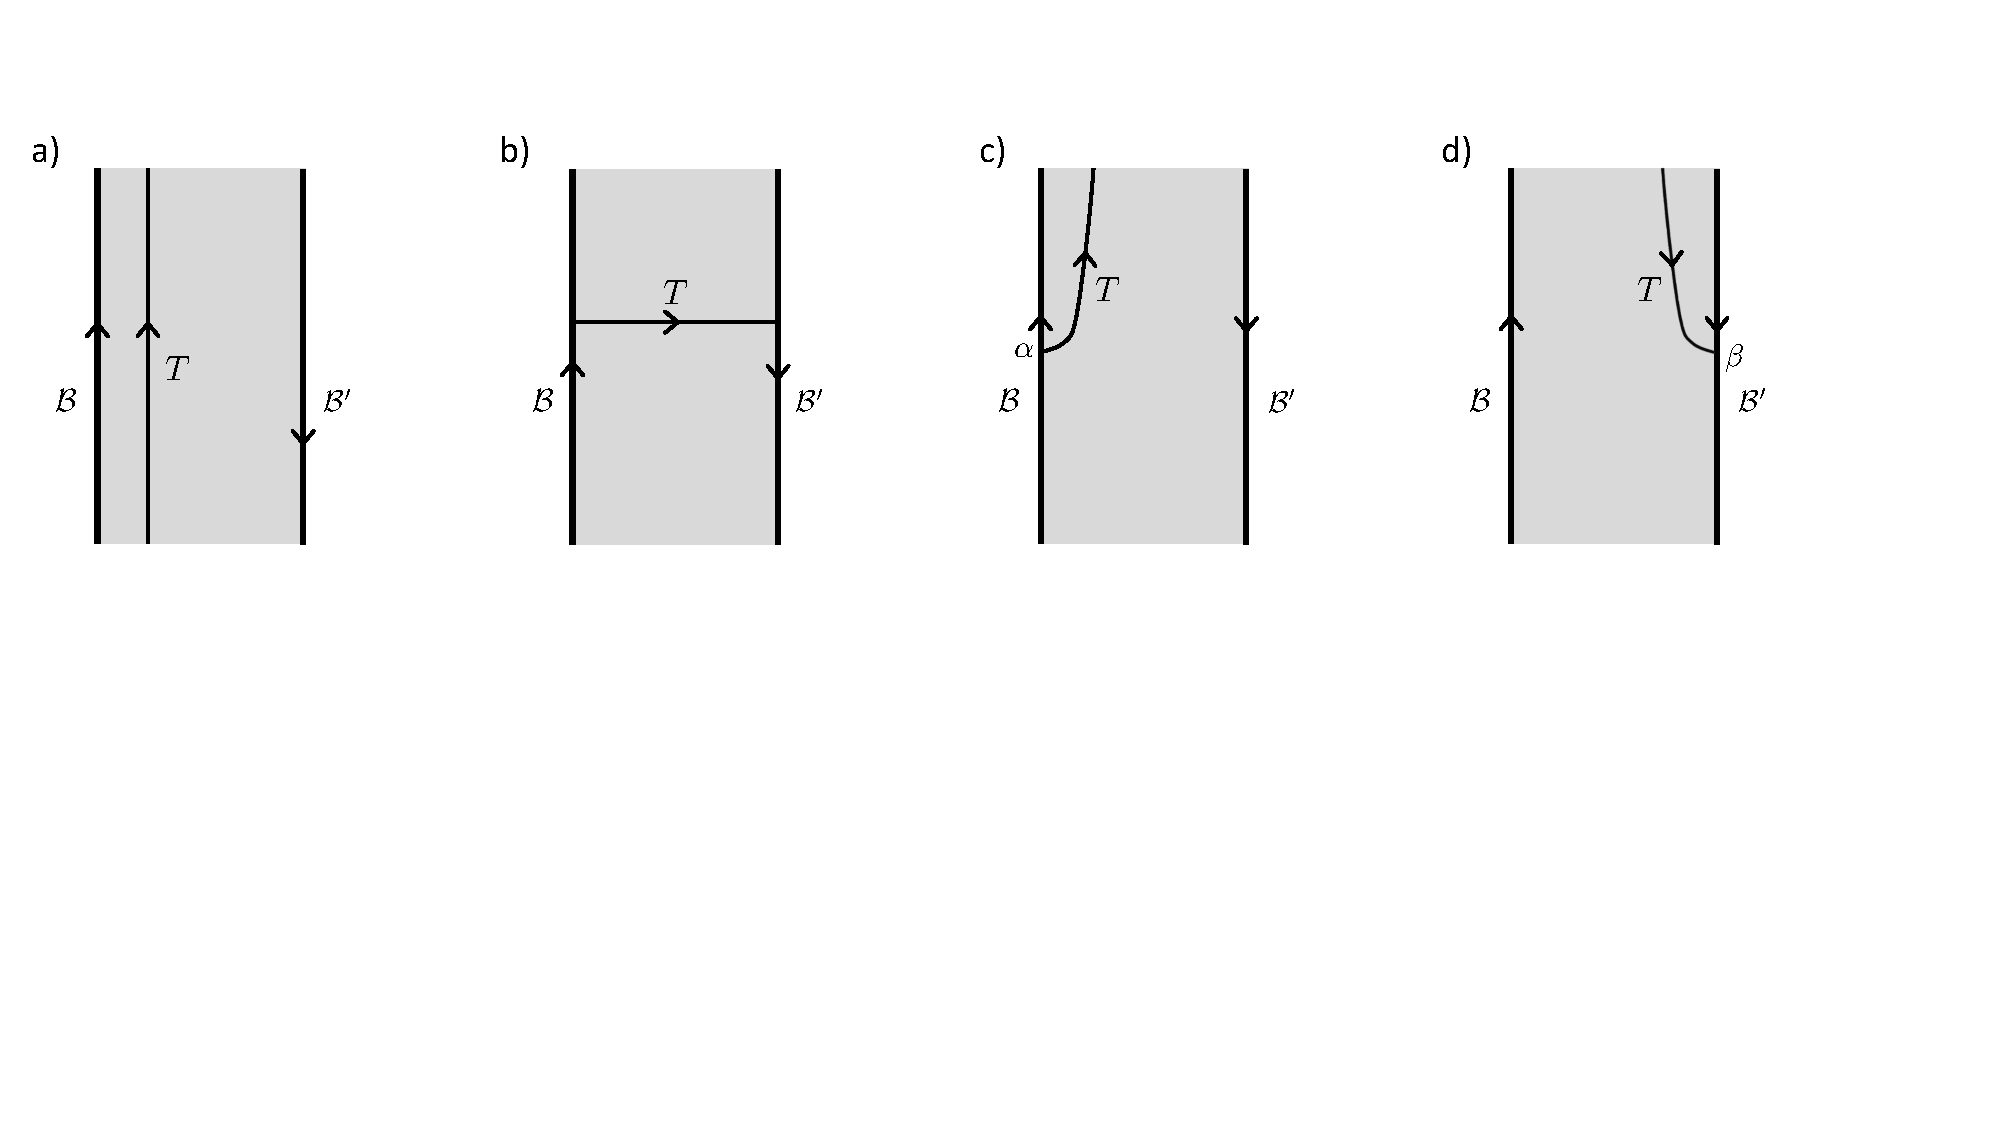
\includegraphics[width=6.2in]{Example1.pdf}
 \end{center}
\caption{\small (a) 与条带左边界平行、且定向与之相容的线算符 $T$。把 $T$ 向左移动，它把标记为 $\B$ 的边界条件映为复合边界条件 $T\B$。这就是把线算符视为膜或边界条件范畴上的函子，正如几何朗兰兹纲领的通常表述那样。(b) 在几何朗兰兹对偶的解析进路中，同一个线算符 $T$ 水平横穿条带，并在端点处带有某些额外数据，于是成为作用在物理态上的算符。(c) 与 (d) 这些图意在阐明 (b) 中左右两端所需的额外数据。在左端点有一个元素 $\alpha\in \Hom(\B,T\B )$，在右端点有一个元素 $\beta\in\Hom(T\B',\B')$。 \label{example1}}
\end{figure} 


 \begin{figure}
 \begin{center}
   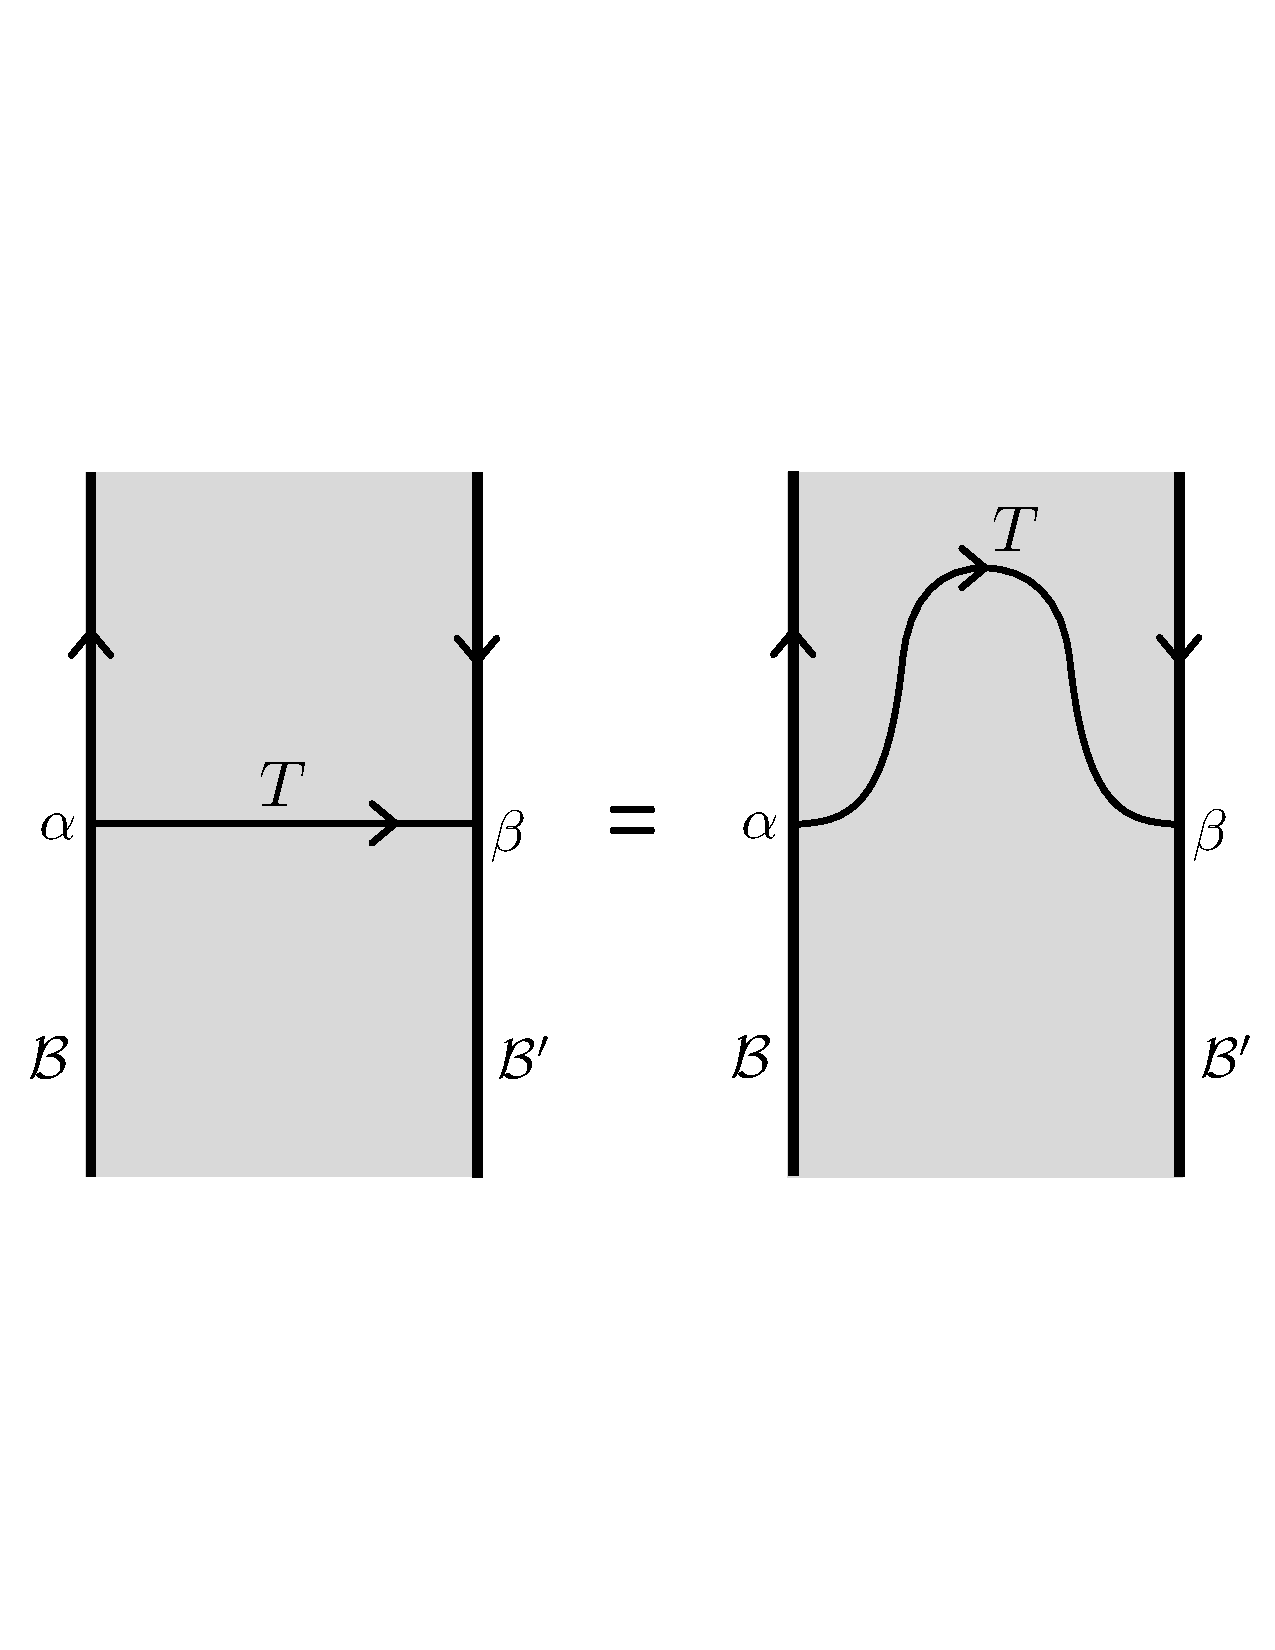
\includegraphics[width=3.4in]{Example2.pdf}
 \end{center}
\caption{\small 本图说明正文中所述的一个代数操作。从下往上读右图，先遇到的是图 \ref{example1}(c,d) 所勾勒的运算，随后是把线算符的乘积 $T'T$ 融合为“恒等”，即融合为平凡线算符。 \label{example2}}
\end{figure} 




在几何朗兰兹对偶的解析进路中 \cite{EFK,EFK2}，Hecke 算符成为作用在量子态希尔伯特空间上的普通算符，而不再是作用在范畴上的更抽象的函子。不出所料，这种意义上的 Hecke 算符的规范场论解释，依据的仍是与前面相同的 't Hooft 线算符，只是用法略有不同。在图 \ref{example1}(b) 中，我们考虑与前面相同的线算符，只不过它现在从图的左侧延伸到右侧。在线算符终止于条带边界的左右两个端点处，必须补充某些额外数据。\zy{译者按（无外部依据）：原文的 strip 指图中画成条带的二维流形 $\Sigma$，其左右两条边界即 $\Sigma$ 的两条边界分支；线算符横穿条带时两端分别落在其上。译文统一作“条带”。}我们暂且假定这些数据已经给定。于是该线算符就成为作用在量子态上的普通算符。从下往上读这幅图：一个 $\Hom(\B',\B)$ 中的元素从底部进入，经过线算符的作用之后，从顶部出来的是一个（可能不同的）$\Hom(\B',\B)$ 中的元素。（若从上往下读，则看到转置算符作用在对偶向量空间 $\Hom(\B,\B')$ 上。）正因为支撑在固定时刻空间中的一维流形上的线算符能够以这种方式充当普通的量子算符，它们传统上\footnote{在粒子物理的传统应用中，没有边界，线算符的支撑集取为闭合回路。此时该算符常被称为圈算符（loop operator）。}才被称为线“算符”。



图 \ref{example1}(c,d) 的目的是解释图 \ref{example1}(b) 中的线算符在左边界或右边界终止处究竟发生了什么。在图 \ref{example1}(c) 中我们看到，线算符的左端点对应一个元素 $\alpha\in\Hom(\B,T\B)$；在图 \ref{example1}(d) 中我们看到，右端点对应一个元素 $\beta\in \Hom(T\B',\B')$。在代数上，带有额外数据 $\alpha,\beta$ 的线算符 $T$ 所对应的算符 $\h T:\Hom(\B',\B)\to \Hom(\B',\B)$ 可以描述如下。对 $\psi\in \Hom(\B',\B)$，有 $\alpha\circ\psi\circ\beta\in \Hom(T\B',T\B)=\Hom(\B',T'T\B)$。再利用线算符构成一个代数、且平凡线算符出现在乘积 $T'T$ 中这两点，便得到映射 $w:\Hom(\B',T'T\B)\to \Hom(\B' ,\B)$。最后，$\h T(\psi)=w\circ\alpha\circ\psi\circ\beta$。这一连串代数操作对应图 \ref{example2} 的画面。对于由线算符 $T$ 或 $T_{R,p}$ 连同端点数据 $\alpha,\beta$ 构造出的 $\H$ 上的算符，我们有时将其记作 $\h T_{\alpha,\beta}$ 或 $\h T_{R,p,\alpha,\beta}$。

\begin{yizhu}[译者按：函子与算符两种图像]
本节的论证可以概括为两个层次的对照。在 Beilinson--Drinfeld 的表述中 \cite{BD}，Hecke 函子作用在 $D$-模或凝聚层的范畴上；在规范场论图像中 \cite{KW}，它对应作用在 $A$-膜范畴上的函子，并由 't Hooft 线算符具体实现。到了 EFK 的解析版本 \cite{EFK,EFK2}，同一个线算符不再是沿边界铺设，而是横穿条带，并在左右两端接上角数据 $\alpha,\beta$，于是成为作用在量子态希尔伯特空间上的普通算符（图 \ref{example1}(b)）。两种图像并不矛盾：把线算符移到边界上便得到函子（图 \ref{example1}(a)），把它的两端接到左右边界上便得到算符；式 $\h T(\psi)=w\circ\alpha\circ\psi\circ\beta$ 正是这一转换的代数表达。
\end{yizhu}


 \begin{figure}
 \begin{center}
   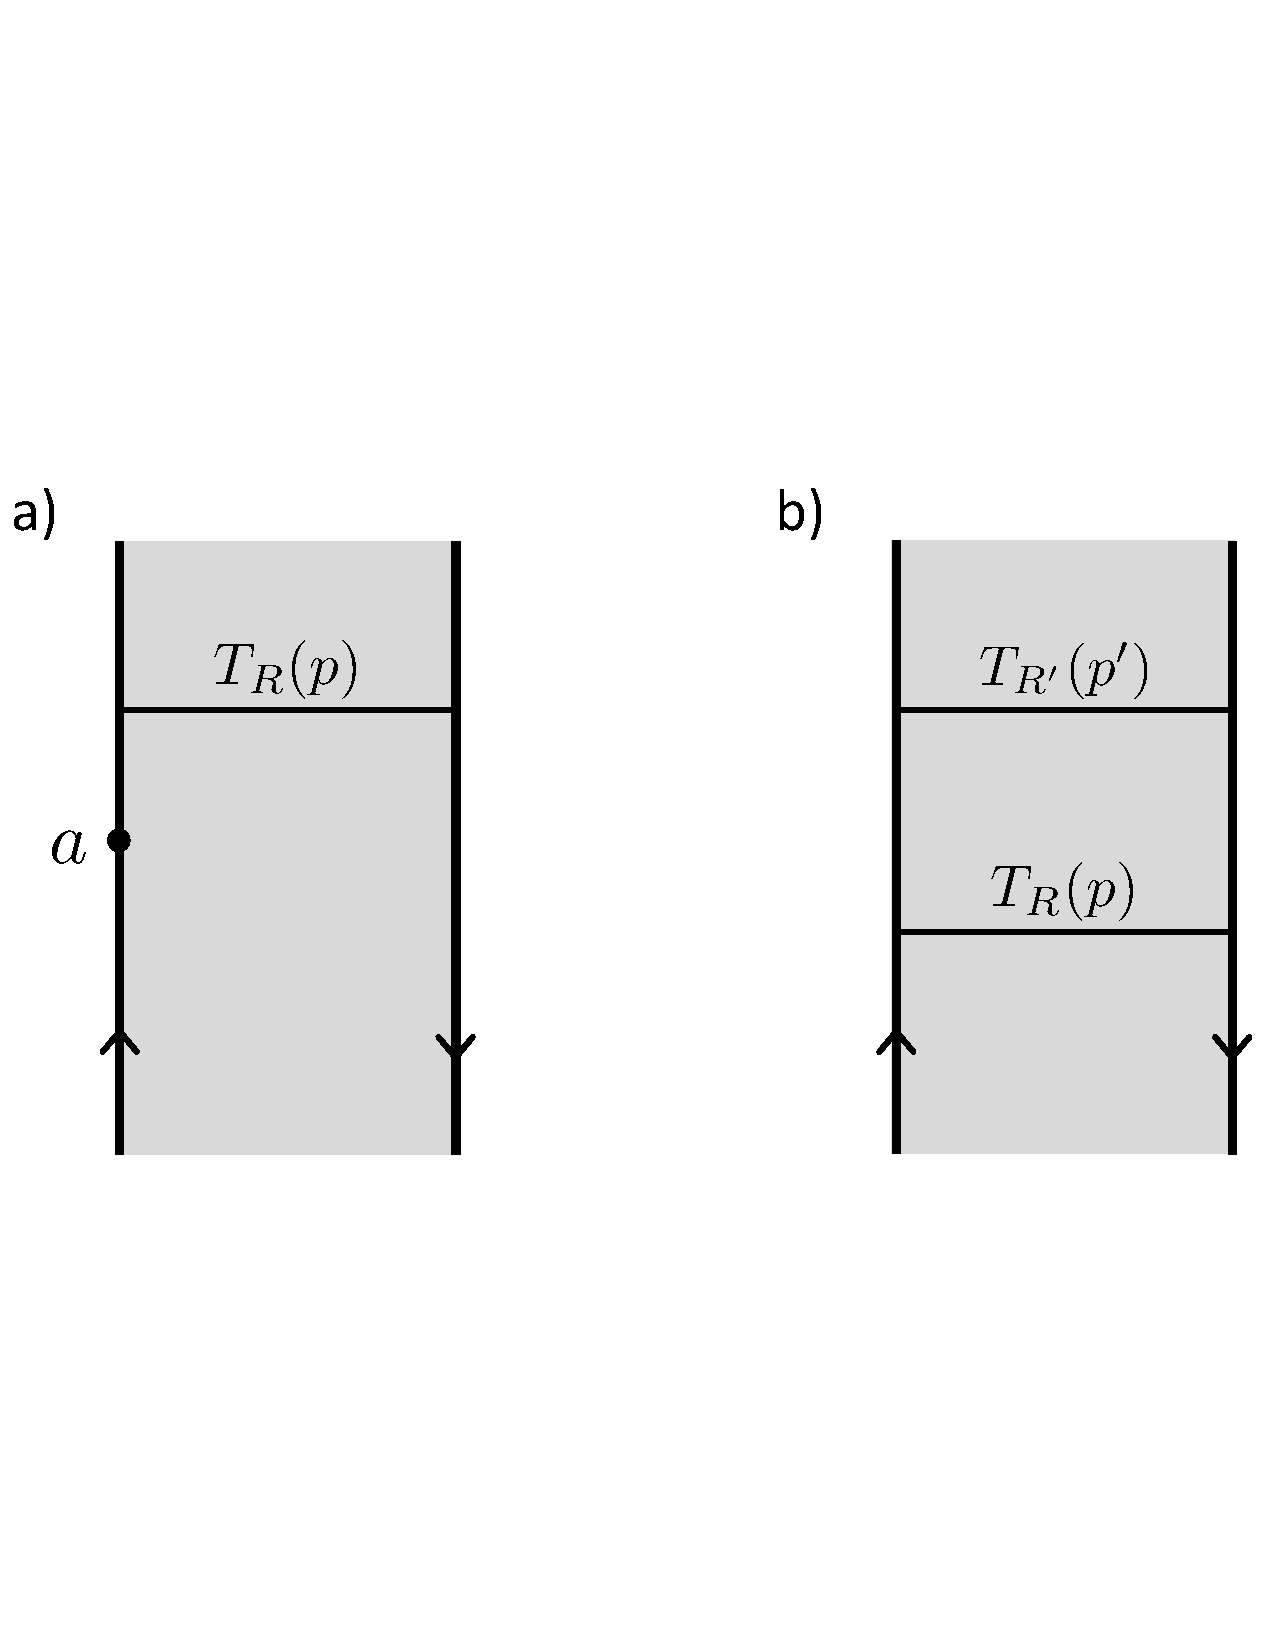
\includegraphics[width=3.4in]{Example3.pdf}
 \end{center}
\caption{\small 证明量子化 Hitchin 哈密顿量彼此交换的论证，可以稍作改动，用来证明线算符（视为量子态空间上的实际算符）与量子化 Hitchin 哈密顿量交换，并且彼此交换。在两种情形下（分别如 (a) 与 (b) 所示），关键都在于：由于额外维度的存在，两个算符可以毫无奇异地互相上下滑过。 \label{example3}}
\end{figure} 


 \begin{figure}
 \begin{center}
   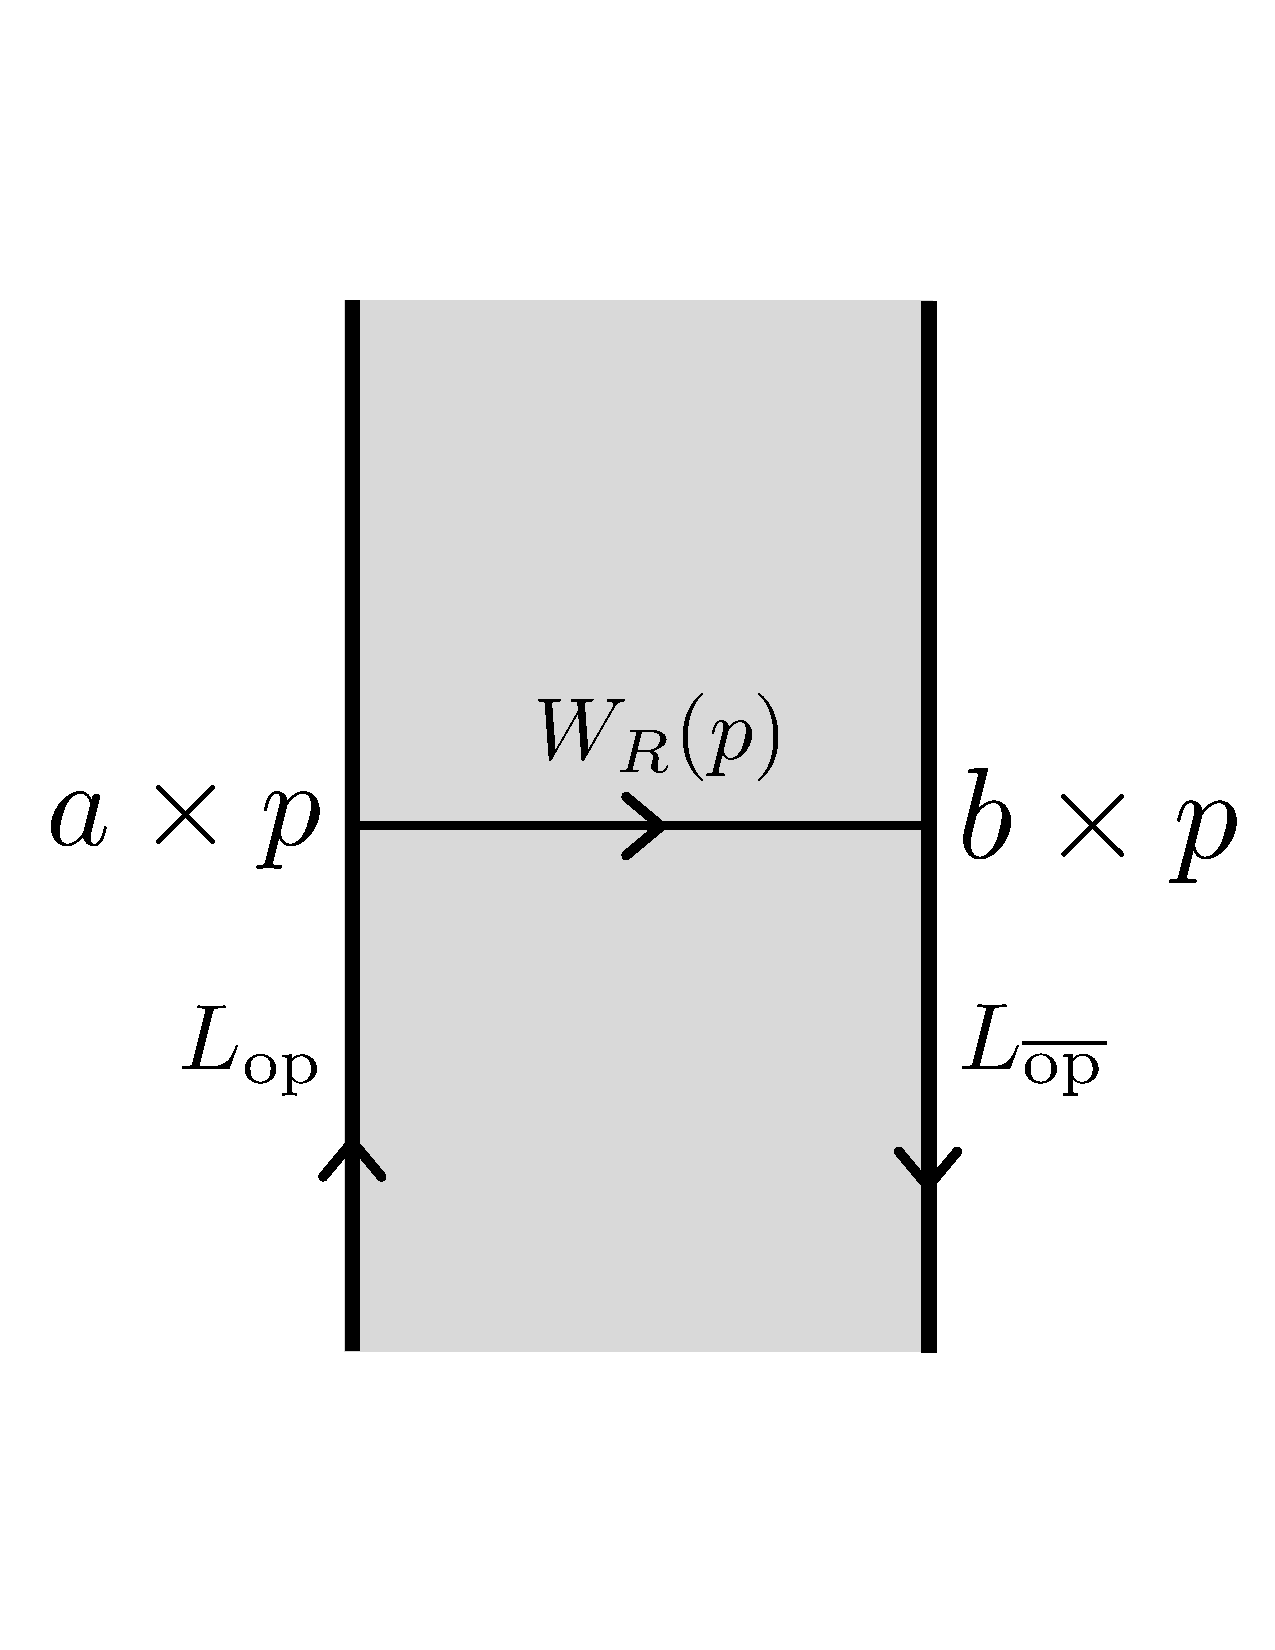
\includegraphics[width=2.1in]{Example4b.pdf}
 \end{center}
\caption{\small 为计算 't Hooft/Hecke 算符的本征值，人们考虑描述从 $a\times p$ 到 $b\times p$ 的平行移动的对偶 Wilson 算符，其中 $p$ 是 $C$ 中的一点，$a,b$ 是 $\Sigma$ 左右边界上的点。 \label{example4}}
\end{figure} 

我们将特别关注这样的元素 $(\alpha,\beta)$：它们起源于四维线缺陷落在四维边界条件上的局部端点，而这些四维边界条件分别是 $\B$ 与 $\B'$ 的提升。正如第 \ref{background} 节所言，我们所考虑的边界条件的四维提升不是拓扑的；它们分别是全纯-拓扑的与反全纯-拓扑的。因此，对应于 $\alpha$ 的局部端点将全纯地依赖 $p$，而对应于 $\beta$ 的局部端点将反全纯地依赖 $p$。注意，线缺陷在四维中的实际路径无关紧要，只要它在拓扑上等价于一条笔直路径即可。真正重要的只是端点在 $C$ 中的位置。

't Hooft 算符或 Hecke 算符（如 \cite{EFK,EFK2} 那样视为量子态上的算符）的主要性质之一是：它们彼此交换，并且与量子化 Hitchin 哈密顿量交换。这可由我们先前用来证明 Hitchin 哈密顿量彼此交换的同一推理得到。't Hooft 算符 $T_{R,p}$ 与 Hitchin 哈密顿量 $H_{\P,\alpha}$ 交换，因为可以假定 $\alpha$ 的支撑集与点 $p$ 不相交，从而让 $T_{R,p}$ 与 $H_{\P,\alpha}$ 毫无奇异地互相上下滑过（图 \ref{example3}(a)）。同样，对互不相同的点 $p,p'\in C$，'t Hooft 算符 $T_{R,p}$ 与 $T_{R',p'}$ 交换（图 \ref{example3}(b)）。取极限 $p'\to p$ 便知，即使 $R\not= R'$，$T_{R,p}$ 与 $T_{R',p}$ 也交换。

\subsection{Wilson 算符及其本征值}\label{wilop}

由于 't Hooft 算符与 Hitchin 哈密顿量交换，它们可以在同一组基下对角化，即态基 $\psi_{u,\veps},$ $u\in \Upsilon,$ $\veps\in \T_u$，其中 $\Upsilon=L_\op\cap L_\bop$（第 \ref{inccenter} 节）。事实上，我们可以用电–磁对偶来确定 't Hooft 算符的本征值。't Hooft 算符 $T_{R,p}$ 对偶于 Wilson 算符 $W_{R,p}$，后者由 $G^\vee_\C$ 的同一个表示 $R$ 标记，并支撑在同一点 $p\in C$。't Hooft 算符是“无序”（disorder）算符，其微观定义涉及某种奇异性。\zy{“无序算符”（disorder operator）与 Wilson 算符这类“有序算符”（order operator）相对：它不能只由沿回路的经典和乐给出，而要在支撑附近规定场的奇异性或单值。't Hooft 在讨论夸克禁闭时引入了这种算符，见 G. 't Hooft, ``On the phase transition towards permanent quark confinement,'' \emph{Nucl. Phys.} \textbf{B138} (1978) 1。} Wilson 算符则不同：它在经典层面上用和乐（holonomy）定义，如下所述。在四维流形 $M$ 上相应的规范场论中（对我们而言，$M=\Sigma\times C$），有一个带联络 $\cA=A+\i \phi$ 的 $G^\vee_\C$ 丛 $E^\vee_\C\to M$，我们可以给它联系一个向量丛 $E^\vee_R=E^\vee_\C\times_{G^\vee_\C} R$。该丛上的诱导联络仍简记为 $\cA$。Wilson 算符由联络 $\cA$ 在 $E^\vee_R$ 上的和乐构造，一般沿某条带定向的路径 $\gamma\subset M$ 积分。若 $\gamma$ 是闭合回路，则取绕 $\gamma$ 的和乐的迹，这样就得到一个在许多物理应用中很重要的 Wilson 算符版本。

然而，要计算由横跨条带的 't Hooft 线算符（图 \ref{example1}(b)）所定义的算符的本征值，我们需要考虑同样横跨条带的对偶 Wilson 算符（图 \ref{example4}）。这个 Wilson 算符不是支撑在闭合回路上，而是支撑在一条路径 $\gamma\subset \Sigma\times p$ 上，该路径从条带左边界上的 $a\times p$ 延伸到右边界上的 $b\times p$。

此时，和乐最好理解为从 $a\times p$ 处的纤维 $E^\vee_R$ 到该丛在 $b\times b$ 处的纤维的线性变换。\zy{译者按（无外部依据）：原文此处作 $b\times b$，据上下文及下一式 (\ref{lintr})，应为 $b\times p$；这是原文笔误，译文照录并在此说明。}于是，按这些纤维的显然记号，$W_{R,p}$ 是一个线性变换
\be\label{lintr} W_{R,p}:E^\vee_{R,a\times p}\to E^\vee_{R, b\times p}.\ee
为了更对称地处理条带的左右两边缘，方便的做法是引入与 $R$ 对偶的表示 $R'$，并把 $W_{R,p}$ 视为某个表示上的线性函数。于是有
\be\label{bintr} W_{R,p}\in \Hom(E^\vee_{R,a\times p}\otimes E^\vee_{R',b\times p},\C). \ee

至此，我们得到的是向量空间上的一个线性函数，而不是联络的复值函数；只有后者才能量子化而得到量子算符。要得到联络的复值函数，我们需要给出向量 $v\in E^\vee_{R,a\times p}$、$w\in E^\vee_{R',b\times p}$。此时 $W_{R,p}(v\otimes w)$ 就是一个复值函数，可以量子化而得到算符。

第 \ref{localoper} 节描述了构造合适向量的一种自然方式。在式 (\ref{linmap}) 中，我们对带有伴丛 $E^\vee_R$ 的全纯 oper 描述了一个“最高权截面” $s_R:K_C^{(N-1)/2}\to E^\vee_R$。因此，若给定向量 $v\in K_{C,p}^{(N-1)/2}$，便可定义 $s_R(v)\in E^\vee_{R,p}$。类似地，若 $E^\vee_{R'}$ 是反全纯 oper，则有 $\bar s_{R'}:\bar K_C^{(N-1)/2}\to E^\vee_{R'}$，从而对 $w\in K_{C,p}^{(N-1)/2}$，有 $\bar s_{R'}(w)\in E^\vee_{R',p}$。注意，对偶的表示对 $R,R'$ 具有相同的 $N$ 值。

若丛 $E^\vee_R\to \Sigma\times C$ 在左边界上是全纯 oper、在右边界上是反全纯 oper，我们就可以在左边界上应用这一构造的全纯版本、在右边界上应用其反全纯版本，从而得到
\be\label{wintr}W_{R,p,v\otimes w}=W_{R,p}(s_{R}(v)\otimes \bar s_{R'}(w)). \ee
这最终是联络的一个复值函数，可以量子化而得到物理态上的 Wilson 算符。我们把这个算符称为 $W_{R,p,v\otimes w}$。在这一记号中，我们利用了如下事实：式 (\ref{wintr}) 的右端只通过组合 $v\otimes w$ 依赖于 $v$ 与 $w$。我们用同一记号表示经典和乐（或其矩阵元）与相应的量子算符，希望这不会造成严重混淆。

由于 $B$-模型局域化在平坦联络上，这个算符的对角化是平凡的。\zy{局域化（localization）指拓扑扭化理论的路径积分只由满足经典运动方程的特殊构型贡献。二维 $B$-模型依赖于靶空间的复结构，其路径积分局域化在常数映射上（E. Witten, ``Mirror manifolds and topological field theory,'' in \emph{Essays on Mirror Manifolds}, 1992; arXiv:hep-th/9112056）；在本文中，这些常数映射对应 $C$ 上的平坦联络。}满足边界条件、在边界上取定中心部分的平凡化、并模去规范变换的平坦联络，与使 Hitchin 哈密顿量对角化的通常态基 $\psi_{u,\varepsilon}$（$u\in\Upsilon,$ $\varepsilon\in \T_u$）一一对应。Wilson 算符在这组基下是对角的。量子算符 $ W_{R,p,v\otimes w}$ 在给定基向量 $\psi_{u,\varepsilon}$ 上的本征值，正是相应的经典函数在与 $\psi_{u,\varepsilon}$ 对应的经典解上的取值。这个值就是向量 $s_{R}(v)$ 与 $\bar s_{R'}(w)$ 在对偶向量空间 $E^\vee_{R,p}$ 与 $E^\vee_{R',p}$ 中的自然对偶配对 $(s_R(v), \bar s_{R'}(w))$。之所以如此，是因为 $\Sigma\times C$ 上的平坦联络实际上是从 $C$ 拉回的。

中心 $\zZ(G^\vee)$ 通过 $(s_\ell, s_r)\to (b s_\ell, s_r)$ 作用在物理希尔伯特空间 $\H$ 上（第 \ref{opergauge} 节）。这会把 $\h W_{R,p}$ 的本征值乘上一个单位根，而这个单位根正是中心元素 $b$ 在表示 $R$ 中的值。例如，若 $G^\vee=\SL(n,\C)$ 且 $R$ 是 $n$ 维表示，则 $\h W_{R,p}$ 的本征向量以 $n$ 元组的形式出现，形如 $\lambda\exp(2\pi \i k/n)$，$\lambda\in\C$，$k=0,1,\cdots, n-1$。这与下述事实相对偶：在 $A$-模型一侧，希格斯丛模空间具有由特征类 $\zeta\in H^2(C,\pi_1(G))$ 标记的若干连通分支。对 $G^\vee=\SL(n,\C)$，共有 $n$ 个分支，它们被与 $\h W_{R,p}$ 对偶的 't Hooft 算符 $\h T_{R,p}$ 循环置换，从而导致相同的谱结构。一般地，$\zZ(G^\vee)$ 在 $R$ 上的作用，映照出 $\h T_{R,p}$ 置换模空间各分支的方式。

定义算符 $W_{R,p}$ 所需的全纯与反全纯角数据（corner data），恰恰由向量 $v\in K_C^{(N-1)/2}$、$w\in \bar K_C^{(N-1)/2}$ 构成。对 $\SL(n,\C)$ 的 $n$ 维表示，有 $N=n$。我们预期，为对偶的 't Hooft 算符定义全纯与反全纯角数据也需要同样的数据。


这些可以说是最简单的 Wilson 算符，我们称之为主 Wilson 算符（principal Wilson operator）。然而，若表示 $R$ 限制到 $\g^\vee$ 的主 $\su(2)$ 子代数上时可约，则可以使用更一般的对象 $s_{R,n}:Q_n\otimes K_C^{(n-1)/2}\to E^\vee_R$（式 (\ref{holmap})）。于是，取 $v\in Q_n \otimes K_C^{(n-1)/2}$、$w\in \bar Q_{n'}\otimes K_C^{(n'-1)/2}$（其中 $n$ 与 $n'$ 可以独立选取），便可定义 $W_{R,p,n,n',v\otimes w}=W_{R,p}(s_{R,n}(v)\otimes \bar s_{R',n'}(w))$，它同样可以解释为一个量子力学算符。更一般地，我们还可以考虑 $W_{R,p,n,n',v\otimes w} $ 关于 $p$ 的全纯与反全纯导数。考虑 $n-1$ 个全纯导数与 $n'-1$ 个反全纯导数就足够了；这足以定义一组完备的 Wilson 算符，因为这相当于把线性形式 $W_{R,p}:E^\vee_{R,a\times p}\otimes E^\vee_{R',b\times p}\to \C $（式 (\ref{bintr})）作用到一组向量上，而按第 \ref{localoper} 节的分析，这组向量构成 $W_{R,p}$ 所作用的那个有限维向量空间的一组基。

如果继续求导会怎样？取 $n$ 个全纯导数或 $n'$ 个反全纯导数，我们就会遇到 Wilson 算符 $W_{R,p,n,n',v\otimes w} $ 所满足的微分方程。用来定义这些 Wilson 算符的全纯与反全纯截面 $ s_{R,r}$ 与 $\bar s_{R',n'}$，作为 $p$ 的函数满足某些全纯与反全纯微分方程（第 \ref{localoper} 节与附录 \ref{somex}），相应的 Wilson 算符也满足同样的方程。


在定义了作用在物理希尔伯特空间 $\H$ 上的算符之后，自然要问它们满足什么代数。在体空间（bulk）中，线算符的乘积模拟 $G^\vee $ 的表示的张量积。因此，若 $R_i\otimes R_j\cong \oplus_k N^k_{ij}R_k$，其中 $N^k_{ij}$ 是向量空间，则相应的平行 Wilson 算符的分解为 $W_{R_i} W_{R_j}=\oplus_k N^k_{ij} W_k$。对于把 Wilson 算符理解为作用在边界条件上的函子这一观点，这正是恰当的关系，如图 \ref{example1}(a) 所示。原则上，由这一代数可以重构非阿贝尔群 $G^\vee $ 的结构。然而，对于此处所讨论的把 Wilson 算符作为量子态上的算符这一观点，情况有所不同。若相乘的是两个主 Wilson 算符——它们与相应表示中的最高权向量相联系——情形最为简单。由于两个表示 $R_1$ 与 $R_2$ 中最高权向量的张量积是张量积 $R_1\otimes R_2$ 中的最高权向量，两个主 Wilson 线算符的乘积仍是主 Wilson 线算符，对应于一个表示 $R_3$，其最高权是 $R_1$ 与 $R_2$ 的最高权之和。若相乘更一般的 Wilson 算符 $W_{R,p,n,n',v\otimes w}$ 及其导数，我们就会看到非阿贝尔群的结构。

用 $S$-对偶数据定义的对偶 't Hooft 算符，自然具有与 Wilson 算符相同的本征值。主要的困难在于精确辨识出适当的 $A$-模型端点。我们将在第 \ref{dualhooft} 节转向这一问题。

我们以如下评述结束关于 Wilson 算符的讨论。在四维规范场论中，oper 边界条件最有启发的实现涉及 Nahm 极点 \cite{GWknots}。与早先假定的较直接进路 \cite{KW}（其中边界条件只通过在边界上指定 $\cA$ 的 $(0,1)$ 或 $(1,0)$ 部分来定义）相比，oper 边界条件的 Nahm 极点描述有两个优点：它直接导致第 \ref{localoper} 节所讨论的局部约束；并且它还为通过 $\B_\cc$ 与 $A$-模型描述的对偶给出了简单的解释。若采用 oper 边界条件的 Nahm 极点描述，则复联络 $\cA$ 沿边界是奇异的，因而在定义横穿条带的经典和乐 $W_R$ 以及相应的量子算符时，需要某种重整化。这种重整化相当于作一个复规范变换，以消去 Nahm 极点奇异性。


   


% ch07: 原文 GLDraft_D.tex 行 1383–1765；§4.3
% 只译散文（标题、正文、图题、脚注）；公式、\label、\ref、\eqref、\cite、图文件名保持不变。

\subsection{对偶 't Hooft 算符}\label{dualhooft}

 \begin{figure}
 \begin{center}
   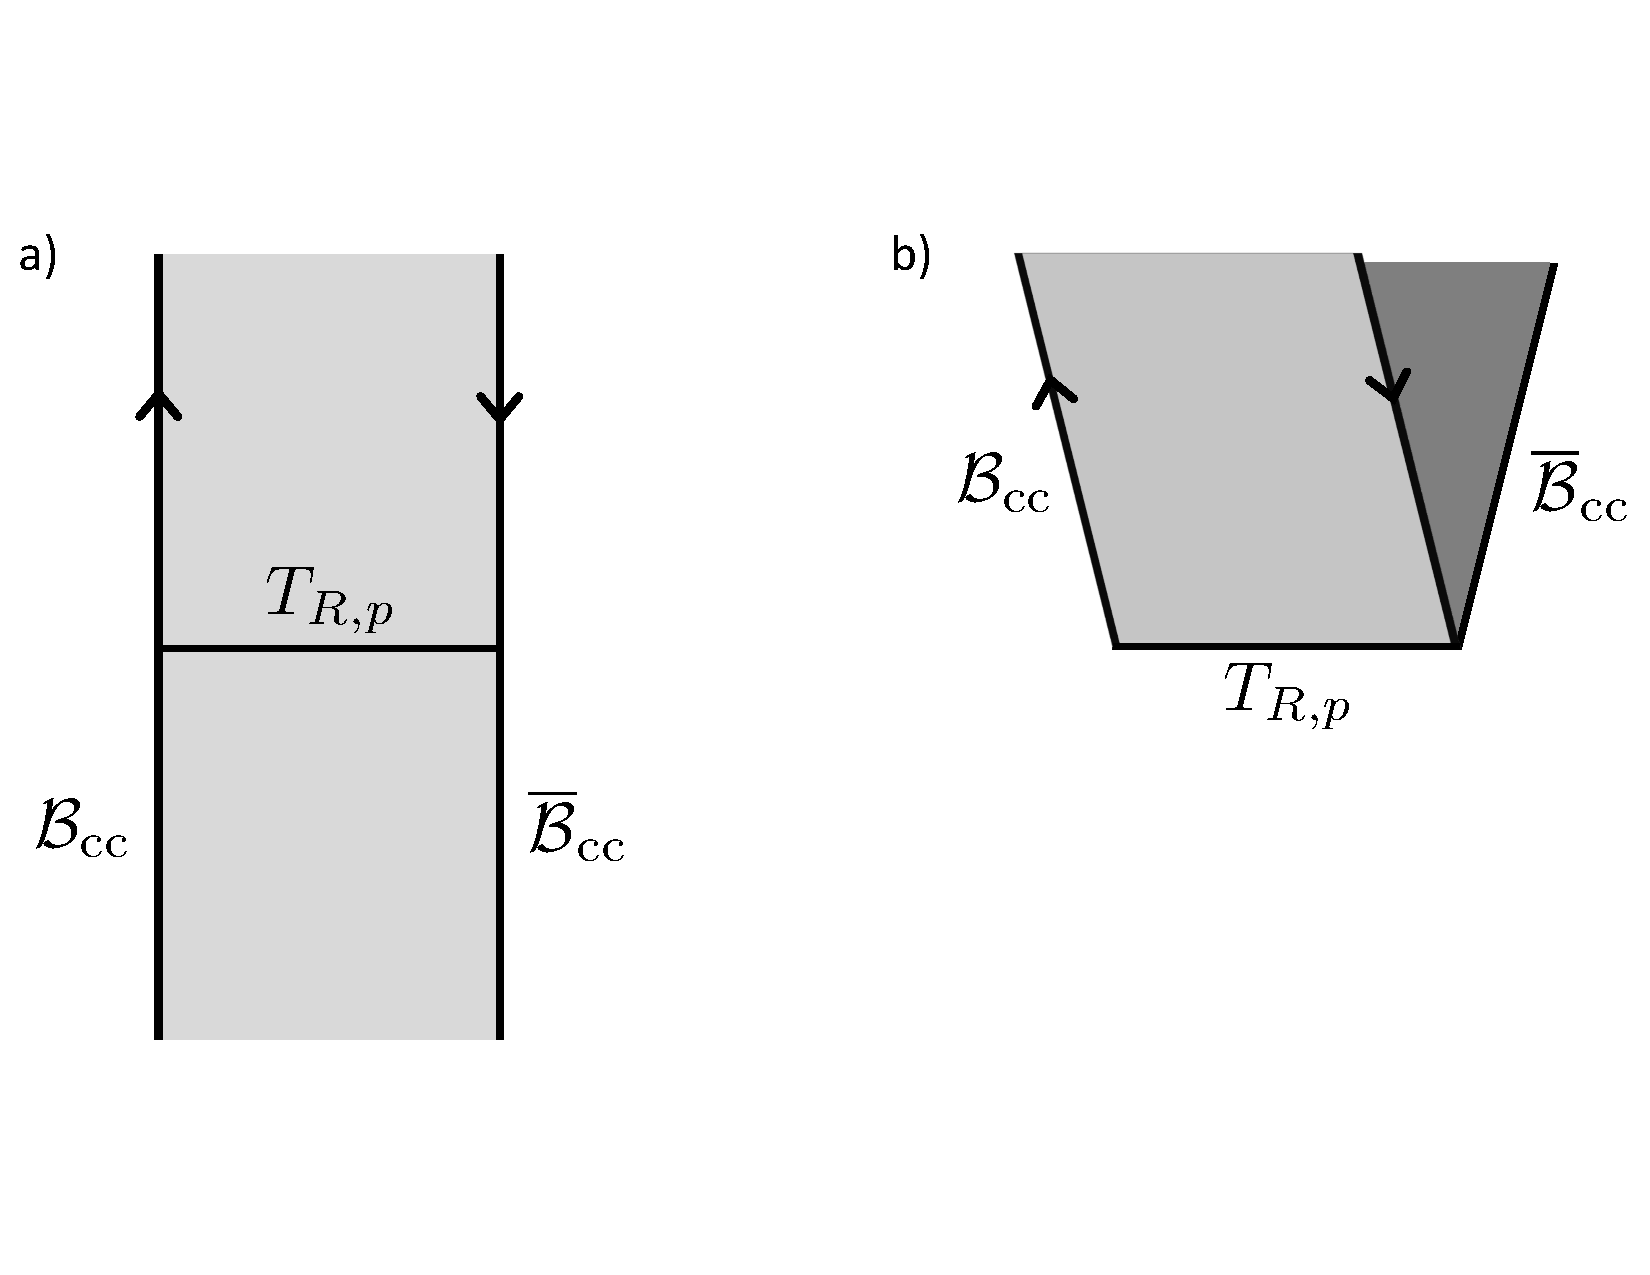
\includegraphics[width=3.6in]{Example7.pdf}
 \end{center}
\caption{\small (a) 把 't Hooft 算符视为从 $\M_H(G,C)$ 的 $A$-模型到自身的界面。(b) 经“折叠”（folding）后，同一个 't Hooft 算符被解释为两张 $\M_H(G,C)$ 之积中的一张膜，它在该乘积中给出一个边界条件；两份辛形式大小相等而符号相反。\label{example7}}
\end{figure} 

\subsubsection{'t Hooft 算符与 Hecke 修正}\label{THO}

一个 't Hooft 算符 $T_{R,p}$（图 \ref{example7}(a)）会使场 $(A,\phi)$ 以及相应的希格斯丛 $(E,\varphi)$ 发生跳跃：'t Hooft 算符紧下方的希格斯丛 $(E,\varphi)$ 一般与紧上方的希格斯丛 $(E',\varphi')$ 不同构。二者之差就是所谓的 Hecke 修正。Hecke 修正的类型由 't Hooft 算符的磁奇异性决定，后者按对偶群 $G^\vee$ 的不可约表示 $R$ 的选取来分类。丛与希格斯丛的 Hecke 修正已在 \cite{KW} 中向物理学家作了说明，\cite{More} 第 4 节给出了更详细的讨论。这里我们只作非常简短的概述。\zy{'t Hooft 算符是磁荷线算符，由对偶群 $G^\vee$ 的不可约表示 $R$ 标记；Wilson 算符是电荷线算符，由所在理论规范群的表示标记。本文的对偶一侧规范群为 $G^\vee$，故 $W_{R,p}$ 也由 $G^\vee$ 的同一表示 $R$ 标记。参见 G. 't Hooft, Nucl. Phys. B138 (1978) 1 及 \cite{KW}。}

全纯 $G_\C$ 丛 $E$ 在点 $p$ 处的 Hecke 修正，是这样一个新丛 $E'$：它带有一个在 $p$ 之外与 $E$ 的同构，但该同构不能延拓到 $p$ 上。$E'$ 的截面 $w$ 就是 $E$ 的截面，只不过允许它在 $p$ 处有指定类型的极点，或受约束使某些分量在 $p$ 处有指定类型的零点，或两者兼有。

例如，设 $E$ 是秩 2 的全纯向量丛，在 $p$ 附近取平凡化，使 $E$ 的截面是一对全纯函数 $\begin{pmatrix}f\cr g\end{pmatrix}$；那么 $E$ 在 $p$ 处的一个 Hecke 修正的例子，是这样一个新丛 $E'$：其截面是一对 $\begin{pmatrix}f\cr g\end{pmatrix}$，其中 $f$ 在 $p$ 处全纯，而 $g$ 允许在 $p$ 处有单极点。这个例子可稍作推广，给出以 $\bCP^1$ 参数化的一族 $E$ 在 $p$ 处的 Hecke 修正。我们只需取一对不全为零的复数 $u,v$，代表 $\bCP^1$ 中一点，并允许 $E'$ 的截面具有与这对数成比例的极点部分：
\be\label{thep} w= \frac{1}{z}\begin{pmatrix}u\cr v\end{pmatrix}+{\mathrm{regular}}, \ee
其中 $z$ 是 $p$ 处的局部参数。

$E$ 与 $E'$ 之间的关系是互反的：与其说我们通过允许某一类型的极点而从 $E$ 得到 $E'$，不如说我们通过要求某一类型的零点而从 $E'$ 得到 $E$。若 't Hooft 算符 $T_{R,p}$ 能把 $E$ 映为 $E'$，则对偶的 't Hooft 算符（与对偶表示相联系）能把 $E'$ 映为 $E$。
 
                                                                    

希格斯丛 $(E,\varphi)$ 的 Hecke 修正实际上对 $\varphi$“什么也没做”。意思是：$(E,\varphi)$ 的 Hecke 修正，就是一个 $E$ 的 Hecke 修正 $E'$，使得 $\varphi:E\to E\otimes K_C$ 作为映射 $E'\to E'\otimes K_C$ 全纯。在秩 2 丛的例子中，希格斯场局部为 $\varphi=\varphi_z\,\d z$，其中 $\varphi_z$ 是 $2\times 2$ 的全纯函数矩阵。要使 $\varphi$ 作为映射 $E'\to E'\otimes K_C$ 全纯，充分必要条件是：若 $w$ 是式 (\ref{thep}) 所刻画的 $E'$ 的截面，则 $\varphi w$ 的极点部分应是 $\begin{pmatrix}u\cr v\end{pmatrix}$ 的倍数；换言之，$\begin{pmatrix}u\cr v\end{pmatrix}$ 必须是矩阵 $\varphi_z(p)$ 的本征向量。一般情形下这一条件并不满足，因此 $E$ 的大多数 Hecke 修正都不能作为 $(E,\varphi)$ 的 Hecke 修正。若 $\varphi_z(p)$ 非幂零，则它有两个不同的本征向量，希格斯丛 $(E,\varphi)$ 在 $p$ 处有两个这种类型的可能 Hecke 修正；若 $\varphi_z(p)$ 幂零但不为零，则它只有一个本征向量，这种类型的可能 Hecke 修正也只有一个；只有当 $\varphi_z(p)=0$ 时，$(E,\varphi)$ 才与 $E$ 本身一样，在 $p$ 处有同一个 $\bCP^1$ 族的这种类型的可能 Hecke 修正。

刚刚描述的这类 Hecke 修正可以从两种不同的角度来看。它们对偶于 $G^\vee=\U(2)$ 的二维表示。该群自对偶，因此上述讨论适用于 $G=\U(2)$ 的规范场论。换一种说法，同一个 Hecke 修正对偶于 $G^\vee=\SU(2)$ 的二维表示。此时对偶群为 $G=\SO(3)$。在这一应用中，由于秩 2 丛 $E$ 与 $E'$ 并不以 $\SO(3)$ 为结构群，前述讨论应以相应的伴丛 $\ad(E)$ 与 $\ad(E')$ 重新表述。

在这个例子中，设 $\delta$ 为 $\varphi(p)$ 作用在 $\begin{pmatrix}u\cr v\end{pmatrix}$ 上的本征值：
\be\label{defdelta} \varphi(p) \begin{pmatrix}u\cr v\end{pmatrix}=\delta \begin{pmatrix}u\cr v\end{pmatrix}.\ee
当 $E$ 与 $E'$ 的选取变化时，$\delta$ 全纯地变化。它定义了这类 Hecke 修正空间上的一个全纯函数。由于 $\varphi(p)$ 的本征值为 $\pm \delta$，我们有
\be\label{delchar} \delta^2=-\det \varphi(p),\ee
其中 $\det\varphi(p)$ 是 Hitchin 哈密顿量的线性组合。$\delta$ 的符号区分与给定希格斯场相容的两种 Hecke 修正。









\subsubsection{Hecke 对应}\label{HC}

't Hooft 算符 $T_{R,p}$ 可以视为 $\M_H(G,C)$ 的 $A$-模型到自身的界面。这不过是同义反复；在图 \ref{example7}(a) 中，我们在 $T_{R,p}$ 的上方与下方都看到 $\M_H(G,C)$ 的 $A$-模型，因此可以把 $T_{R,p}$ 视为这个 $A$-模型的两份副本之间的界面。事实上，由于 $T_{R,p}$ 的超对称性质，这个界面是 $(B,A,A)$ 型的。使用类似于图 \ref{folding} 的折叠技巧会很方便。我们不必把 $T_{R,p}$ 与 $\M_H(G,C)$ 的 $A$-模型中的界面相联系，而可以把它与乘积 $\M_H(G,C)\times \M_H(G,C)$ 的 $A$-模型中的一张 $(B,A,A)$ 型膜或边界条件 $\B_{R,p}$ 相联系（图 \ref{example7}(b)）。这里 $\M_H(G,C)\times \M_H(G,C)$ 的辛结构为 $\omega_K\boxplus (-\omega_K)$，其中一个因子取负号，因为折叠会反转辛结构的符号。

让我们具体看看，对于第 \ref{THO} 节所述的基本例子——$R$ 为 $G^\vee=\SU(2)$ 的二维表示——$\B_{R,p}$ 会是什么样子。它的复维数是多少？若 $C$ 的亏格为 $g$，则 $G_\C$ 丛 $E$ 的选取依赖于 $3g-3$ 个复参数。选取可由 $T_{R,p}$ 作用于 $E$ 而得到的 $E'$，又多出一个复参数。但我们还必须约束希格斯场 $\varphi$，使 $\begin{pmatrix}u\cr v\end{pmatrix}$ 是 $\varphi(p)$ 的本征向量。因此 $\varphi$ 的选取涉及 $3g-4$ 个参数，而不是 $3g-3$ 个。结论是：$\B_{R,p}$ 的支撑 $Z_{R,p}$ 的维数为 $6g-6$，于是 $Z_{R,p}$ 在 $\M_H(G,C)\times \M_H(G,C)$ 中是中维的（middle-dimensional）。由于 $Z_{R,p}$ 是中维的，且是 $(B,A,A)$ 型膜的支撑，它必是复拉格朗日子流形。膜 $\B_{R,p}$ 的秩为 1，因为 $T_{R,p}$ 由 $E$ 产生 $E'$ 所用的 Hecke 变换（若存在）一般是唯一的。简言之，$\B_{R,p}$ 是一张 $(B,A,A)$ 型的秩 1 拉格朗日膜。

我们可以说得更具体些，因为 $\B_{R,p}$ 显然在 $\varphi$ 的标度变换下不变，而这一变换对应于 $\M_H(G,C)\times \M_H(G,C)$ 的 $\C^*$ 对称性。我们可以给出一个简单描述，其意义与用稠密开集 $T^*\M(G,C)$ 近似 $\M_H(G,C)$ 相同。（正如量子化的一般讨论那样，我们预期在 $\lmark^2$ 理论中这一近似是足够的。）$Z_{R,p}$ 与 $\M(G,C)\times \M(G,C)\subset T^*\M(G,C)\times T^*\M(G,C)$ 的交，是参数化配对 $E,E'$ 的簇 $X_{R,p}$，其中 $E'$ 可由 $E$ 经 $p$ 处 $R$ 型 Hecke 变换得到。$Z_{R,p}$ 的 $\C^*$ 不变性意味着它可以被认定为 $X_{R,p}$ 的余法丛\footnote{若子流形 $U\subset M$ 局部由若干坐标 $q_1,\cdots, q_r$ 的零点定义，则它在 $T^*M$ 中的余法丛由令这些坐标以及与它们泊松交换的动量等于零来定义。}。$X_{R,p}$ 在这种情形下称为 Hecke 对应，而 $Z_{R,p}$ 是希格斯丛的 Hecke 对应。
\zy{几何朗兰兹中，Hecke 对应 $X_{R,p}$ 给出 Hecke 函子（沿对应拉回、再推回），Hecke 本征层即其本征对象；希格斯丛的 Hecke 对应 $Z_{R,p}$ 是 $X_{R,p}$ 在 $T^*\M(G,C)\times T^*\M(G,C)$ 中的余法丛。参见 \cite{BD} 与 E. Frenkel, arXiv:hep-th/0512172。}
   
对偶于 $G^\vee=\SU(2)$ 二维表示的这个 't Hooft 算符特例相对简单，因为给定丛 $E$ 在给定点 $p$ 处的可能 Hecke 修正构成一维空间。一般而言，$T_{R,p}$ 能在 $p$ 处对 $E$ 作出的 Hecke 修正，其空间的维数依赖于 $R$；若 $R$ 是 $G^\vee$ 的最高权很大的表示，该维数可任意大。当维数足够大时，每个 $E'\in \M(G,C)$ 都可由 $E$ 经 $T_{R,p}$ 得到，而得到它的方式构成一个正维数的复流形 $\Phi_{E',E,R,p}$。在这种情形下，$Z_{R,p}$ 相当复杂。它有一个希格斯场为零的分支（若 $E'$ 由 $E$ 经一个权非常高的普通 Hecke 修正产生，则不存在非零的 $\varphi:E\to E\otimes K$ 作为映射 $E'\to E'\otimes K$ 全纯），还有希格斯场非零的其他分支（可以选取 $E$ 的权任意高的 Hecke 修正，使得 $\varphi:E'\to E'\otimes K$ 全纯）。$\B_{R,p}$ 的 $\CP$ 丛限制到各分支上并不只是秩 1 的。例如，限制到希格斯场为零的那个分支上，这个 $\CP$ 丛形式地（也就是说，在恰当处理奇点之后）就是 $\Phi_{E',E,R,p}$ 的上同调。
\zy{原文所说的 $\CP$ 丛指膜上的 Chan–Paton 丛，其秩即膜的秩；“并不只是秩 1”指它在某些分支上秩可大于 1。参见 J. Polchinski, \emph{String Theory}, Vol. 1（CUP, 1998）。}
 
\subsubsection{'t Hooft 线算符作为量子态上的算符}\label{lineq}
   
在相当一般的条件下，若辛流形 $M$ 能通过膜量子化得到希尔伯特空间 $\H$，则 $M\times M$ 中的 $A$-膜 $\B$（并在“角”处带有附加数据，详见下文）可解释为 $\H$ 上的量子算符。\cite{GW} 第 4 节对此作了一般讨论。一般说来，很难得到这种算符的显式描述。但这里我们处于一个答案简单的特殊情形。这是因为 $M=\M_H(G,C)$ 实际上就是余切丛 $T^*\M(G,C)$，而所关心的膜支撑在子簇 $X_{R,p}\subset \M(G,C) \times \M(G,C)$ 的余法丛上。
 
作用在 $T^*\M(G,C)$ 的量子化上的相当一般的算符 $\O$，可以用 $\M(G,C)\times \M(G,C)$ 上的半密度 $F(x,y)$ 作为积分核来表示。$\O$ 对态 $\Psi$ 的作用为
\be\label{actst} \O\Psi(x)=\int_{\M(G,C)}\d y \, F(x,y) \Psi(y). \ee
与 't Hooft 算符 $T_{R,p}$ 相联系的量子算符 $\h T_{R,p}$ 应具有何种积分核？式 (\ref{actst}) 中的点 $y$ 与 $x$，在图 \ref{example7}(a) 中对应于线算符 $T_{R,p}$ 紧下方与紧上方的场 $(A,\phi)$。因此它们对应于丛 $E$、$E'$，其中 $E'$ 可由 $E$ 经 $p$ 处 $R$ 型 Hecke 修正得到。于是在经典极限下，$F(x,y)$ 是支撑在 $X_{R,p}$ 上的分布，而 $X_{R,p}$ 参数化这样的配对 $(E,E')$。我们首先考虑的最简单情形，是 $F(x,y)$ 在垂直于 $X_{r,p}$ 的方向上为 delta 函数。更一般地，就其对法向的依赖而言，$F(x,y)$ 可正比于 delta 函数在法向变量中的任意阶导数。\zy{$F$ 与 $\Psi$ 各为半密度，$F(x,y)\Psi(y)$ 是 $y$ 方向的密度，故积分不依赖坐标选取；几何量子化中预量子化态本就是半密度。参见 Bates–Weinstein, \emph{Lectures on the Geometry of Quantization}（AMS, 1997）。}

一般而言，人们会预期对“$F(x,y)$ 支撑在经典对应 $X_{R,p}$ 上”这一论断有量子修正。然而在当前情形没有修正，因为被量子化的辛流形是余切丛 $T^*\M(G,C)$，而对应 $Z_{R,p}$ 是 $T^*\M(G,C)\times T^*\M(G,C)$ 中的余法丛。余切丛与余法丛的标度不变性意味着核 $F(x,y)$ 不能依赖于 $\hbar$，并可在半经典极限下计算。

我们应补充说明，为什么在这里依据标度对称性作论证是正当的。膜量子化一如既往，是在某个适当的复化中研究 $T^*\M(G,C)$。类似地，在膜量子化中研究 $Z_{R,p}$，需要把它复化到 $T^*\M(G,C)\times T^*\M(G,C)$ 的某个复化之中。膜量子化中的标度论证实际上涉及复化的标度变换。这种论证在当前情形有效，是因为 $T^*\M(G,C)$ 作为余切丛的结构、以及 $Z_{R,p}$ 作为余法丛的结构，确实延拓为它们复化上的同类型全纯结构。

我们还应当澄清“半经典极限”的含义。波函数是半密度而非函数、相应地 $F(x,y)$ 是 $\M(G,C) \times \M(G,C)$ 上的半密度，这一论断本身已包含单圈修正。说 $F(x,y)$ 可以半经典地计算，意思是除此之外没有别的量子修正。

根据 Etingof、Frenkel 与 Kazhdan \cite{EFK2}，对偶于 $\SU(2)$ 二维表示的 Hecke 算符由一个积分核定义，该核可分解为全纯因子与反全纯因子之积。这种全纯因子化在 $A$-模型中是可预期的。全纯因子 $f$ 将来自图 \ref{example7}(a) 中 $T_{R,p}$ 的左端点，等价地来自图 \ref{example7}(b) 的左下角；反全纯因子 $\t f$ 将来自右端点或右下角。
我们把 't Hooft 算符视为 $\M_H(G,C)\times \M_H(G,C)$ 中一张 $(B,A,A)$ 型的秩 1 膜，其 $\CP$ 丛平凡。一般而言，这种支撑在拉格朗日子流形 $L$ 上的膜与典范余迷向 $A$-膜之间的角空间为 $H^0(L,K_L^{1/2})$。't Hooft 算符对应于支撑为 Hecke 对应 $Z_{R,p}$ 的膜。因此在这一情形，全纯的角是全纯截面 $f\in H^0(Z_{R,p},K^{1/2}_{Z_{R,p}})$。类似地，反全纯的角是元素 $\t f\in H^0(\bar Z_{R,p},\bar K^{1/2}_{\bar Z_{R,p}})$，其中 $\bar Z_{R,p}$ 是取相反复结构的 $Z_{R,p}$。
 
 
  
$f$ 与 $\t f$ 的乘积 $\mu = f \t f$ 将是 $Z_{R,p}$ 上的半密度。我们将说明，这些数据恰好是定义分布核 $F(x,y)$ 所需。若 $f$ 与 $\tilde f$ 是自 $X_{R,p}$ 拉回的，我们将得到 delta 函数核。若它们对 $Z_{R,p} \to X_{R,p}$ 的纤维有多项式依赖，我们将得到 delta 函数各阶导数的线性组合。

为了描述 delta 函数分布，我们选取一些局部坐标。用 $\M(G,C)$ 上的坐标 $\vec x=x_1,\cdots, x_{3g-3}$ 参数化 Hecke 变换的输入。我们将用 $|\d \vec x|$ 表示半密度 $(\d x_1 \cdots \d x_{3g-3} \d \bar x_1 \cdots \d \bar x_{3g-3})^{1/2}$，对随后引入的其他变量也作同样的理解。给定 $\vec x$ 后，Hecke 变换的输出跑遍一个 $\bCP^1$ 的副本，我们称之为 $\bCP^1_x$，并用复变量 $z$ 参数化它。$\bCP^1_x $ 在 $\M(G,C)$ 中的复余维为 $3g-4$。$\bCP^1_x$ 可局部由条件 $\vec n=0$ 定义，其中 $\vec n=(n_1,\cdots, n_{3g-4})$ 是 $\M(G,C)$ 中 $\bCP^1_x$ 的法丛 $N$ 上的局部全纯坐标。于是核可写为
\be\label{nuff} 
F(x,y)= b(z,\bar z,x, \bar x)|\d\vec x ||\d z \d \vec n |\delta(\vec n,\vec{\bar n})
\ee
其中 $\d \vec n=\d n_1 \d n_2\cdots \d n_{g-4}$，delta 函数由 $\int \d \vec n \d \vec{ \bar n}\delta(\vec n,\vec{\bar n})=1$ 定义。由后一关系可知，在法丛上作坐标变换时，delta 函数按 $(\d \vec n \d \vec{\bar n})^{-1}$ 变换；这意味着可能的核与下列对象一一对应：
\be\label{luff} \mu = b(z,\bar z,x, \bar x)|\d\vec x| |\d z(\d \vec n)^{-1}|. \ee
希格斯丛的 Hecke 对应 $Z_{R,p}$ 局部由上文引入的坐标 $\vec x$ 与 $z$（它们参数化丛的 Hecke 对应 $X_{R,p}$）以及参数化希格斯场选取的附加变量 $\vec m$ 来参数化。由于 $Z_{R,p}$ 是 $X_{R,p}$ 的余法丛，变量 $\vec m$ 与式 (\ref{nuff}) 中出现的法丛坐标 $\vec n$ 对偶。因此我们可以把 $(\d\vec n)^{-1}$ 换成 $\d \vec m$，而可能的 delta 函数核与 $Z_{R,p}$ 上的半密度一一对应：
\be\label{luff1} \mu = b(z,\bar z,x, \bar x)|\d\vec x \d z\d \vec m|^2. \ee
其中 $b$ 与 $\vec m$ 无关。

这一讨论可直接推广到 delta 函数法向导数的线性组合。一个涉及 delta 函数法向导数的核
\be\label{nuff2} 
F(x,y)= b(x, \bar x,z,\bar z, \partial_{\vec n}, \partial_{\vec {\bar n}}) |\d\vec x | |\d z \d \vec n |\delta(\vec n,\vec{\bar n})
\ee
对应于半密度
\be\label{luff2} \mu = b(x, \bar x, z,\bar z,\vec m, \vec {\bar m})|\d\vec x \d z\d \vec m|. \ee
这些半密度定义在 $Z_{R,p}$ 上，且 $b$ 对 $\vec m$ 有多项式依赖。

全纯因子化的核将取 $\mu = f \t f$ 的形式，其中 $f$ 与 $\t f$ 分别是全纯与反全纯的。现在可以看出 $f$ 必须是何种全纯对象。$f$ 必须是 Hecke 对应 $Z_{R,p}$ 上全纯意义下的半密度：$f=v(\vec x, z,\vec m) (\d \vec x\d z\d\vec m)^{1/2}$。用更标准的语言，$f$ 必须是 $H^0(Z_{R,p}, K^{1/2}_{Z_{R,p}})$ 中的元素。如前所述，这正是 $A$-模型中对 $T_{R,p}$ 左端点的答案所应取的形式。类似地，$\t f$ 是 $Z_{R,p}$ 的反典范丛的反全纯截面，这同样符合 $A$-模型的预期。


当且仅当 $Z_{R,p}$ 是 Calabi–Yau 流形时，$K_{Z_{R,p}}^{1/2}$ 存在一个处处非零的特定全纯截面 $\lambda_0$。若这样的 $\lambda_0$ 存在，则定义任何其他全纯角的数据为 $f= g \lambda_0$，其中 $g$ 是 $Z_{R,p}$ 上的全纯函数。特别地，这样的函数 $g$（只具有多项式增长）是 Hitchin 哈密顿量 $H_{\P,\alpha}$ 与式 (\ref{defdelta}) 所定义的全纯函数 $\delta$ 的多项式，但要模去关系 $\delta^2 = -\det \varphi(p)$——该关系把 $\delta^2$ 表示成 $H_{\P,\alpha}$ 的线性组合。非常数多项式 $g(H_{\P,\alpha},\delta)$ 有非平凡的零点，因此 $g\lambda_0$ 处处非零仅当 $g$ 为常数；这表明 $\lambda_0$（若存在）在相差常数倍的意义下唯一。\footnote{更一般地，若 $Z$ 是满足 $b_1(Z)=0$ 的复流形，则 $Z$ 上处处非零、且没有指数增长的全纯函数 $g$ 必为常数。事实上，由 $b_1(Z)=0$，闭 1-形式 $\d g/g$ 恰当，即 $\d g/g=\d w$ 对某个 $w$ 成立，于是 $g=C e^w$（$C$ 为非零常数）；除非 $g$ 为常数，否则 $g$ 有指数增长。$G_\C$-丛的 Hecke 对应满足 $b_1(X_{R,p})=0$。$G_\C$ 希格斯丛的 Hecke 对应是 $X_{R,p}$ 的余法丛，因此 $b_1(Z_{R,p})=0$。}\zy{译者按（无外部依据）：$K^{1/2}_Z$ 有处处非零全纯截面，当且仅当 $K_Z$ 平凡——若 $s$ 是这样的截面，则 $s^2$ 即 $K_Z$ 的处处非零全纯截面，反之亦然。}
形如 $g \lambda_0$ 的角（其中 $g$ 是 Hitchin 哈密顿量与 $\delta$ 的多项式），恰好与 Wilson 线的角相匹配——后者由 $s$、$Ds$ 以及对偶于 Hitchin 哈密顿量的可观测量的多项式构成。


这样的 $\lambda_0$ 确实存在，这归功于 Beilinson 与 Drinfeld 的一个结果 \cite{BD}，该结果在 Etingof、Frenkel 与 Kazhdan 的工作 \cite{EFK2} 中很重要。$\lambda_0$ 的性质映照了第 \ref{wilop} 节中最简单的 Wilson 线角 $s$ 的性质。特别地，根据 Beilinson 与 Drinfeld 的结果，$\lambda_0$ 与 $s$ 一样，作为 $K_p^{-1/2}$ 的截面随 $p$ 变化。当然，这样的 $s$ 的镜像的存在性可由电–磁对偶预期。
 
\cite{EFK2} 中使用了一个稍有不同的表述。为说明这一点，让我们回到式 (\ref{luff})：由此可以看出，若 $\mu$ 能全纯因子化，则其全纯因子是全纯形式 $k = w(\vec x,z) (\d \vec x    \d z)^{1/2}  (\d \vec n)^{-1/2}$。我们可以把 $\d z^{1/2} (\d\vec n)^{-1/2}$ 换成 $\d z (\d \vec y)^{-1/2}$，其中 $\vec y=(z,\vec n)$ 参数化 Hecke 变换的输出。换言之，全纯因子化的核将来自一个全纯对象\footnote{由于 $\vec y$ 由 $\vec x$ 与 $z$ 决定，且反过来 $\vec x$ 由 $\vec y$ 与 $z$ 决定，我们同样可以写 $w(\vec y,z)$ 而不写 $w(\vec x,z)$。}
 \be\label{conf} k=w(\vec x,z) (\d \vec x)^{1/2} (\d\vec y)^{-1/2}\d z. \ee 
若把 $k$ 乘以它的复共轭，我们得到
 \be\label{onf}|k|^2= |w(\vec x,z)|^2 |\d\vec x| |\d z\d\bar z| |\d\vec y|^{-1}.\ee
这直接导致 \cite{EFK2} 中所用的定义。量 $|k|^2$ 可视为从 $\vec y$ 中的半密度到 $\vec x$ 中的半密度的映射，取值于可在 $\bCP^1_x$ 上积分的微分形式 $|\d z \d\bar z|$。该积分给出点 $p\in C$ 处的 Hecke 算符：
 \be\label{tonf} H_p=\int_{\bCP^1_x} |k|^2. \ee
  
 
 
在第 \ref{sec:chiral} 节中，我们将通过二维手征代数来解释其中一些陈述。特别地，第 \ref{fft} 节中关于伴随值手征费米子的讨论，是 Beilinson 与 Drinfeld 原始分析的物理学解释。手征代数方法在 $C$ 上是局部的，并有可能延拓到如下情形：联系两个给定丛的 Hecke 修正空间具有正维数。


\subsubsection{仿射 Grassmann 流形}\label{affgr}


至此我们考虑的都是 Hecke 修正的最简单例子。但要把理论进一步发展，人们需要更系统的途径。

作为动机，我们首先考虑秩 $n$ 的全纯向量丛。设 $z$ 是在点 $p\in C$ 处为零的局部全纯参数，$U$ 是 $p$ 的小邻域。$C$ 有一个由两个开集组成的开覆盖，即 $U$ 与 $C'=C\backslash p$（从 $C$ 中挖去 $p$）。在点 $p$ 的小邻域 $U$ 中取 $E$ 的平凡化，并把 $E$ 限制到 $C'$。设 $E_0\to U$ 是秩 $n$ 的平凡向量丛。于是我们得到 $C$ 的一个开覆盖，由开集 $C'$ 与 $U$ 组成，其上分别有向量丛 $E\to C'$ 与 $E_0\to U$。因此可以通过在 $U'=C'\cap U$ 上把 $E$ 与 $E_0$ 用一个规范变换粘合起来，定义新的向量丛 $E'\to C$。例如，我们可以用从 $E_0$ 到 $E$ 的对角规范变换
  \be\label{gtr} g(z) =\begin{pmatrix} z^{d_1} &&&\cr
                                                                      & z^{d_2} &&\cr
                                                                       &&\ddots & \cr
                                                                          &&& z^{d_n}\end{pmatrix},\ee 其中 $d_1,\cdots, d_n$ 为整数。
对于 $G=\U(n)$，适当选取 $d_i$，这就给出一个 $G_\C$-丛的 Hecke 修正的例子，它对偶于 $G=\U(n)$ 的任意不可约有限维表示。
对于 $G=\SU(n)$，只需再要求 $\sum_i d_i=0$，使 $g(z)$ 取值于 $\SL(n,\C)$；对于 $G=\PSU(n)$，则考虑 $d_i$ 取值于 $\frac{1}{n}\Z$，且 $d_i-d_j\in \Z$（这等价于说：若把 $g(z)$ 写在 $\PSU(n)$ 的表示中，则只出现 $z$ 的整数幂）。把所有 $d_i$ 作常数平移 $d_i\to d_i+c$（其中 $c\in \Z$，对 $G=\PSU(n)$ 则 $c\in \frac{1}{n}\Z$）不影响 Hecke 修正的空间，因为这可以通过 $E'\to E'\otimes \O(p)^c$ 补偿。


对任意 $G$，都可作类似构造：把其元素为 $z$ 的各次幂的对角矩阵换成同态 $g(z)= z^\m :\C^*\to T_\C$，其中 $\C^*$ 是挖去原点的 $z$ 平面，$T_\C$ 是 $G_\C$ 的复极大环面，而 $\m$ 推广了上一段中的整数 $d$ 元组 $(d_1,\cdots, d_n)$，它是对偶群 $G$ 的整权，在物理上对应于 't Hooft 算符的磁荷。


至此所描述的是对偶于 $G$ 的任意有限维表示 $R$ 的 Hecke 变换的标准例子；$R$ 由整数 $d_i$ 或 $\m$ 的选取所编码。
这一构造依赖于最初在 $U$ 上对 $E$ 的平凡化的选取。通过改变平凡化的选取，可以得到同一类型 Hecke 修正的整个空间。一旦选定一个参考平凡化，$E$ 在集合 $U$ 上的任何其他平凡化都可由参考平凡化经
某个在 $U$ 上全纯的规范变换 $g'(z)$ 作用得到。与此替代平凡化相应的标准 Hecke 修正，在参考平凡化下由修改后的奇异规范变换 $g'(z) z^\m$ 描述。
 
两个奇异规范变换给出同一个 $E'$，当且仅当它们可以通过从右复合一个定义在 $U$ 上的规范变换 $g''(z)$ 相互联系。于是，$E$ 的两个平凡化给出同一个标准 Hecke 修正，当且仅当相应的规范变换 $g_1'(z)$ 与 $g_2'(z)$ 满足
\begin{equation}
g_1'(z)z^\m = g_2'(z)z^\m g''(z)
\end{equation}
对某个 $g''(z)$ 成立。

这些关系可以借助{\it 仿射 Grassmann 流形} $\Gr_{G_\C}$ 来形式化。习惯上把定义在 $U'$ 上的 $G_\C$ 值规范变换构成的（无穷维）空间记作 $G_\C[{\cal K}]$，并把其中可全纯延拓到 $U$ 的子空间记作 $G_\C[{\cal O}]\subset G_\C[{\cal K}]$。仿射 Grassmann 流形
\begin{equation}
\Gr_{G_\C} \equiv G_\C[{\cal K}]/G_\C[{\cal O}]
\end{equation}
参数化的是奇异规范变换的等价类。我们定义 $\Gr^\m_{G_\C}$ 为 $\Gr_{G_\C}$ 中由粘合函数 $z^\m$ 给出的标准 Hecke 修正所在的轨道：
\begin{equation}
\Gr^\m_{G_\C} \equiv \left[G_\C[{\cal O}] z^\m \right].
\end{equation}
$\Gr^\m_{G_\C}$ 中的每一点都在某个这样的轨道上（对某个 $\m$）。
\begin{yizhu}[译者按：仿射 Grassmann 流形与 Hecke 修正]
原文用 $\Gr_{G_\C}=G_\C[{\cal K}]/G_\C[{\cal O}]$ 来表述 Hecke 修正，其中 ${\cal K}=\C((z))$、${\cal O}=\C[[z]]$ 为形式洛朗级数环与形式幂级数环。直观上，$\Gr_{G_\C}$ 的参数是“在穿孔邻域 $U'$ 上平凡、在 $p$ 处允许有极点”的 $G_\C$-丛粘合数据；$\Gr^\m_{G_\C}$ 则是粘合函数 $z^\m$ 所在的轨道。对 $G=\U(n)$，轨道由 $n$ 元组 $(d_1,\cdots,d_n)$ 模去整体平移刻画，同时平移所有 $d_i$ 相当于把丛张量以 $\O(p)$ 的某个幂，不改变 Hecke 修正的空间。原文后文 $|d_i-d_j|\leq 1$ 的条件选出的正是极小（minuscule）轨道，故不发生单极子冒泡。介绍见 X. Zhu, “An introduction to affine Grassmannians and the geometric Satake equivalence,” arXiv:1603.05593；用法见 \cite{BD}。
\end{yizhu}


对 $G$ 与 $\m$ 的一般选取，会遇到“单极子冒泡”（monopole bubbling）现象：'t Hooft 算符或 Hecke 算符的磁荷可能发生向下跳跃（这一现象由 \cite{Kron,Pauly} 引入；简短介绍见 \cite{KW} 第 10.2 节）。本质上，轨道 $\Gr^\m_{G_\C}$ 在仿射 Grassmann 流形中不是闭的，其（可能奇异的）闭包包含磁荷更小的其他轨道 $\Gr^{\m'}_{G_\C}$。这会使分析大为复杂化。

对 $G=\U(n)$ 或与之相关的群 $\SU(n)$、$\mathrm{PSU}(n)$，避免单极子冒泡的条件是对所有 $i,j$ 有 $|d_i-d_j|\leq 1$。在把所有 $d_i$ 作常数平移（如式 (\ref{gtr}) 的讨论所述，这不影响 Hecke 修正的空间）之后，为避开单极子冒泡，可以假定 $k$ 个 $d_i$ 为 $-1$，其余为 $0$。
具体地说，这对应于如下类型的 Hecke 修正。设 $E\to C$ 是秩 $n$ 的全纯向量丛，$p\in C$；选取一个 $k$ 维子空间 $V\subset E_p$，定义新向量丛 $E'\to C$，其截面是 $E$ 的截面中允许在 $p$ 处有单极点、且留数落在 $V$ 中的那些。这类 Hecke 修正的空间由 $V$ 的选取参数化，也就是由 $E_p$ 的 $k$ 维子空间构成的 Grassmann 流形参数化。这样的 Hecke 修正对偶于 $G=\U(n)$ 或 $\SU(n)$ 的基本表示的 $k$ 次反对称幂。
在这一情形，$\varphi$ 在 $w$ 的极点部分上表现为 $k \times k$ 矩阵。$\varphi$ 的 $k \times k$ 限制的特征多项式取一般形式 $u(x) = x^k + \delta_1 x^{k-1} + \cdots \delta_k$，其中 $\delta_1,\cdots, \delta_k$ 是某些全纯函数。这些函数与 Hitchin 哈密顿量 $\H_{\P,\alpha}(\varphi)$ 满足多项式关系，这些关系编码了“$u(x)$ 整除 $\varphi$ 的特征多项式”这一约束。




% \subsubsection{Corner data for 't Hooft Line Operators}
%In the brane quantization setup we need to identify good choices of corner morphisms $\alpha$ which can represent supersymmetric 
%endpoints of 't Hooft lines on the deformed Neumann boundary conditions. In a classical approximation, such endpoints are 
%labelled by holomorphic functions on the $Z_{R,p}$ correspondence. In order to compare 't Hooft and Wilson line observables, we 
%need to be able to compare the respective endpoints. 
%
%In the case of $\SO(3)$ and the minimal charge 't Hooft loop, we have identified above a holomorphic observable $\delta$. This represents a holomorphic function on $Z_{2,p}$ which does not descend from a holomorphic function on $\M(G,C)\times \M(G,C)$. Instead, it satisfies the relation $\delta^2 = \frac12 \Tr \varphi^2(p)$. We thus have two candidate ``classical corners'', labelled by holomorphic functions $1$ and $\delta$. 
%
%On the $S$-dual side, we also have two corners: the canonical holomorphic section $s$ and its first derivative $Ds$. We also have a relation $D^2s = t s$ which closely resembles a quantization of the $\delta^2 = \frac12 \Tr \varphi^2(p)$ relation. The resemblance becomes particularly close when we observe that the holomorphic function $\delta$ is actually the Hamiltonian for the infinitesimal deformation $Z_{2,p} \to Z_{2, p + d p}$, 
%i.e. if we let $p$ vary as we compute the difference of complex symplectic forms on $\M_H(G,C)\times \M_H(G,C)$ we obtain $d\delta dp$. 
%Correspondingly, multiplication of a holomorphic function by $\delta$ is the classical approximation to a $D$ derivative acting on a corner. 
%Similar considerations apply to the case of minimal charge 't Hooft loops for $\mathrm{PSU}(n)$. 
%
%Remarkably, the quantum numbers of the classical corners $1$ and $\delta$ do not match the quantum numbers of the Wilson line corners: 
%$s$ is a section of $K_C^{-\frac12}$ while $1$ is not. We will now explain now how such mismatch can be corrected at the semiclassical level. 
%
%\subsubsection{??}
%
%Consider the case of $G=\SO(3)$ and minimal Hecke modification. After selecting a local description in the neighbourhood of $p$, the 
%space of Hecke modifications is $\CP^1$ and we we should thus write 
%\be\label{actst2} \O_{2} \Psi(x)=\int_{\CP^1}|\d z| \left|\frac{\d(H_z \circ x)}{\d y} \right| \, F(z,x) \Psi(H_z \circ x) . \ee
%where $x$ represents $E$, $H_z \circ x$ represents $E'$ and $z$ is a point on $\CP^1$. For later convenience, we inserted an explicit 
%Jacobian factor, comparing the bundle of half-densities in a neighbourhood of $E$ and $E'$.
%
%Next, we impose the constraint that the 't Hooft operator is local on $C$. In particular, the weight give to a specific Hecke modification cannot depend on the structure of the bundle away from $p$, nor on the specific direction of the Hecke modification, as the direction can be changed by a different choice of local trivialization of the bundle $E$. We thus propose 
%\be\label{actst3} \O_{2} \Psi(x)=\int_{\CP^1}|\d z| \left|\frac{\d(H_z \circ x)}{\d y} \right| \, \Psi(H_z \circ x) . \ee
%This proposal actually makes sense because of a rather non-trivial fact: the Jacobian factor transforms as a density on the space of Hecke modifications. 
%
%The Jacobian factor has another remarkable property: it depends on $p$ as a section of $|K_C|^{-1}$. As a consequence, 
%the operator $\O_2$ has precisely the same quantum numbers as the minimal Wilson operator on the dual side, $s \wedge \bar s$. 
%
%As for other important properties of the space of bundles, these properties of the Jacobian are easiest to derive in the model given by the space of 2d connections modulo complexified gauge transformations, where chiral algebra methods become available. We will do so in a dedicated section of the paper. The same methods also allow one to verify the differential equation $D_p^2 O_2 = D_{\P} O_2$ expected from $S$-duality: the 
%'t Hooft line endpoints satisfy an oper differential equation with a classical stress tensor given by the quantum Hitchin Hamiltonians. 
%
%Notice that the other non-trivial corner, obtained as $D_p O_2$, gives an integral-differential operator. This is the sort of operator which one may associate to the quantization of a conormal correspondence with non-trivial corners. 
%
%Important elements of this analysis apply to general gauge group $G$ and magnetic charge $\lambda$. We would seek an integral operators defined tentatively as an integral over some space ${\cal H}_\lambda$ of Hecke modifications:
%\be\label{actst4} \O_{\lambda} \Psi(x)=\int_{{\cal H}_\lambda}|\d z| \left|\frac{\d(H_z \circ x)}{\d y} \right| \,  F(z,x)  \Psi(H_z \circ x) . \ee
%The local change of trivializations act on ${\cal H}_\lambda$. Indeed, a natural choice of ${\cal H}_\lambda$ is the closure of the orbit of 
%the $z^\lambda$ modification under the action of local changes of trivialization. It is thus natural to set $F(z,x)=1$ and hope that 
%the Jacobian will give a reasonably behaved density on the space ${\cal H}_\lambda$. 
%
%Such operators are the natural candidate dual to the leading Wilson line operators $(\bar s_{\bar R_\lambda}, s_{R_\lambda})$
%in the representation $R_\lambda$ labelled by $\lambda$. A very non-trivial check of this proposal would be a comparison of 
%the differential equations satisfied by the two sides. Again, this is ultimately a chiral algebra calculation. 
%
%One can also seek more general integral-differential operators which integrate over ${\cal H}_\lambda$ some combination of derivatives 
%of $\Psi$, possibly generating operators which are $S$-dual to more general $(\bar s_{\bar R_\lambda,\bar n}, s_{R_\lambda,n})$.
%
%


    
 

% ch08: 原文 GLDraft_D.tex 行 1766–1973；§5
% 只译散文（标题、正文、图题、脚注）；公式、\label、\ref、\eqref、\cite、图文件名保持不变。

\section{量子形变的 WKB 条件}\label{wkb}

\subsection{量子态与 Hitchin 纤维化}\label{hitchinwkb}
 \begin{figure}
 \begin{center}
   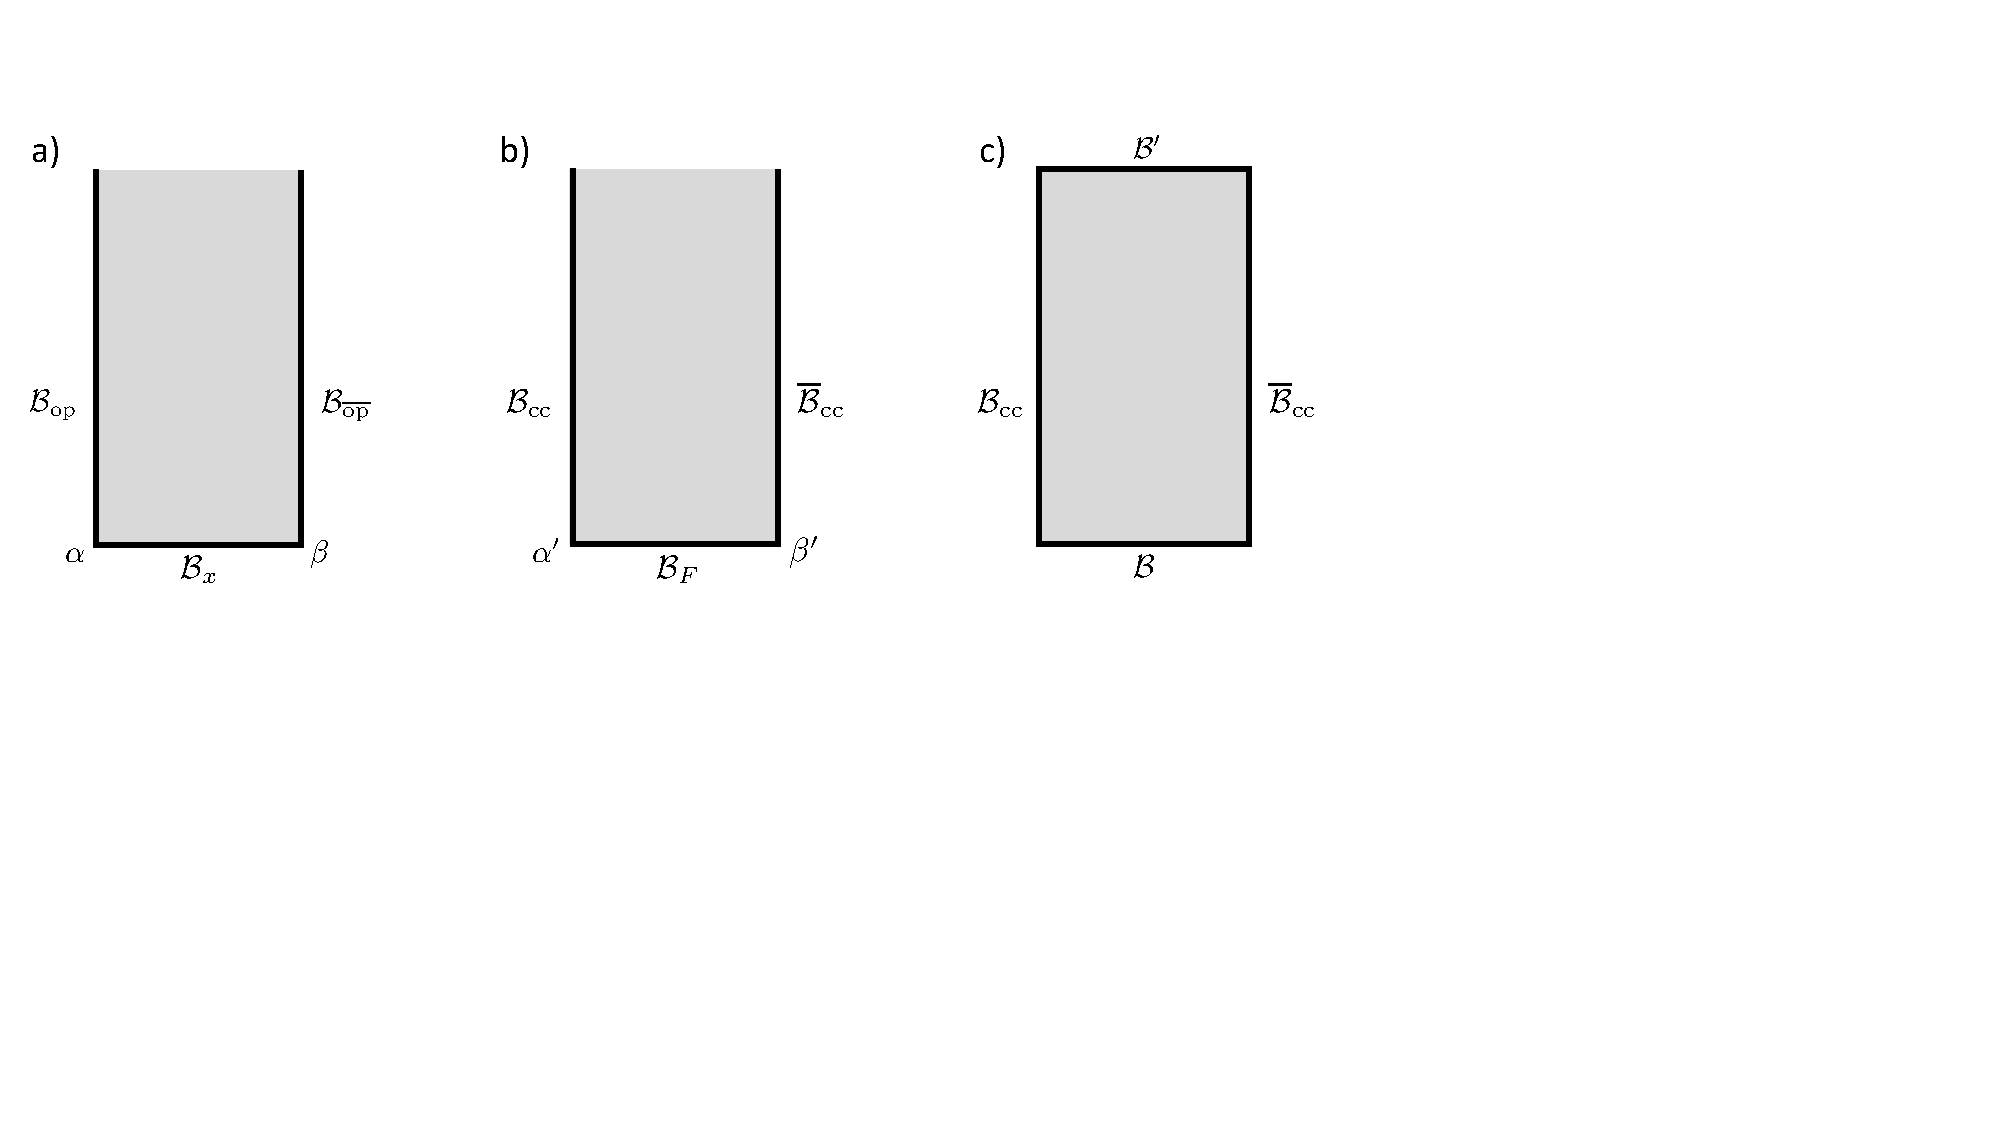
\includegraphics[width=4.7in]{Example6.pdf}
 \end{center}
\caption{\small (a) 支撑在点 $x$ 处的 $B$-膜 $\B_x$，它借助角上的一些数据，定义了 $\H=\Hom(\B_{\bop},\B_{\op})$ 中的一个态。(b) 对偶的 $A$-膜 $\B_F$，支撑在 Hitchin 纤维化的一条纤维 $F$ 上，定义了 $\H=\Hom(\bar\B_\cc,\B_\cc)$ 中的一个态。(c) 关联到 $A$-膜 $\B$ 与 $\B'$ 的态之间的配对（连同角上的数据）。若 $\B$ 与 $\B'$ 中至少有一个具有紧支撑，则该配对有定义；否则可能没有定义。   \label{example6}}
\end{figure} 

关于 Wilson 算符与 Hitchin 哈密顿量的本征函数，还有一种略有不同的看法。设 $x$ 是 $\M_H(G^\vee,C)$ 中对应于平坦 $G^\vee_\C$ 丛 $E^\vee_x\to C$ 的一点，并设 $\B_x$ 是支撑在 $x$ 处的 $B$-膜，带有秩 1（因而必然平凡）的 $\CP$ 丛\zy{$\CP$ 即 Chan--Paton 丛，指膜上的规范丛。参见 H.-M. Chan and J. E. Paton, ``Generalized Veneziano model with isospin,'' \emph{Nucl. Phys.} B10 (1969) 516。}。于是 $\Hom(\B_x,\B_\op)$ 的 0 次部分\footnote{$B$-模型具有守恒的费米子数对称性，微分 $Q$ 的费米子数为 1（即次数为 1）。当 $x\in L_\op$ 时，$\Hom(\B_x,\B_\op)$ 在正次数上也非零，但在本讨论中正次数态没有贡献，因为 $\Hom(\B_\bop,\B_\op)$ 完全位于 0 次。后文讨论 $A$-模型时有类似的说明。}在 $x\in L_\op$ 时（即 $E^\vee_x$ 为全纯 oper 时）同构于 $\C$；否则 $\Hom(\B_x,\B_\op)=0$。类似地，$\Hom(\B_\bop,\B_x)$ 的 0 次部分在 $x\in L_\bop$ 时（即 $E^\vee_x$ 为反全纯 oper 时）为 $\C$，否则为零。当且仅当 $E^\vee$ 同时是 oper 与反 oper 时，我们可以选取非零元素 $\alpha\in \Hom(\B_x,\B_\op)$、$\beta\in \Hom(\B_\bop,\B_x)$，进而定义元素 $\alpha\circ\beta \in \H=\Hom(\B_\bop,\B_\op)$。图 \ref{example6}(a) 描绘了这一情形。膜 $\B_x$ 用来在带形的底边提供边界条件；$\alpha$ 与 $\beta$ 则提供在图形各角定义边界条件所需的“角数据”。以 $\B_x,\alpha,\beta$ 设定“初始条件”的路径积分，定义了系统的一个物理态。这个态就是 Hitchin 哈密顿量与 Wilson 算符所期望的本征态。

通过电–磁对偶，我们可以得到对偶的图像。$\N=4$ 超杨–米尔斯理论在定向二维流形 $C$ 上紧化后，其电–磁对偶在低能下退化为希格斯丛模空间的镜像对称 \cite{BJSV,JWS}。如 \cite{HT} 所解释，这是罕见的情形：镜像对称的 SYZ 解释 \cite{SYZ}——即把镜像对称看作沿一族拉格朗日环面的纤维作 $T$-对偶——在此可以写得非常明确。Hitchin 纤维化是把希格斯丛 $(E,\varphi)$ 映到 $\varphi$ 的特征多项式（characteristic polynomial）\zy{译者按（无外部依据）：原文把 characteristic polynomial 拼作 ``characteristic poiynomial''，多出一个 i，系排印笔误；译文按其本意译作“特征多项式”，不径改原文。}的映射。该映射的纤维是阿贝尔簇（abelian variety），它们关于复结构 $I$ 是复拉格朗日子流形。这尤其意味着，从希格斯丛模空间的实辛结构 $\omega_K=\Im\,\Omega_I$ 来看，它们是拉格朗日子流形。因此，在辛结构为 $\omega_K$ 的 $A$-模型中，Hitchin 纤维化可看作一个 SYZ 纤维化，其纤维是拉格朗日子流形，且一般情形下是环面。沿此纤维化的纤维作 $T$-对偶，把辛结构 $\omega_K$ 的 $A$-模型映到复结构 $J$ 的 $B$-模型。电–磁对偶与这一镜像对称实例的关系，是 \cite{KW} 中的一个重要输入。

特别地，此情形下的镜像对称把支撑在点 $x$ 处的秩 1 膜 $\B_x$ 映为支撑在 Hitchin 纤维化的一条纤维 $F$ 上的膜 $\B_F$，其 $\CP$ 丛是平坦线丛\footnote{\label{canon}一般而言，秩 1 膜的 $\CP$ 丛更典范地是一个 $\Spinc$ 结构，而非线丛。在目前的情形下，由于 $F$ 是阿贝尔簇，因而具有典范的旋量结构，这一区别并不重要。} $\S\to F$。$\alpha\in \Hom(\B_x,\B_\op)$ 与 $\beta\in\Hom(\B_\bop,\B_x)$ 的对偶分别是元素 $\alpha'\in \Hom(\B_F,\B_\cc)$ 与 $\beta'\in \Hom(\b\B_\cc,\B_F)$。元素 $\alpha'\circ\beta'\in \H$ 对应图 \ref{example6}(b) 的图形，它表示 $\H$ 在磁描述下的一个元素；在磁描述中，Hitchin 哈密顿量是作用在 $\M(G,C)$ 上半密度上的微分算子，Wilson 算符则由 't Hooft 算符取代。

膜 $\B_x$ 与 $\B_F$ 都具有紧支撑，其支撑分别是点 $x$ 或 Hitchin 纤维化的一条纤维 $F$。紧支撑使如下一点变得显然：由这些膜（连同角数据）产生的态是可归一化的。不仅如此，紧支撑还意味着，这些态与用任意膜 $\B'$（可能具有非紧支撑，但同样配上适当的角数据）按类似方式构造的态之间，具有良好定义的配对。换言之，只要矩形底部的膜具有紧支撑，由图 \ref{example6}(c) 的矩形构造出的配对就总有定义，而与矩形顶部的膜无关。这大致意味着：带有一组角数据的任意膜定义一个分布态（distributional state），它未必是希尔伯特空间 $\H$ 中可归一化的向量；而具有紧支撑的膜定义一个可与任何分布配对的向量。希尔伯特空间包含于分布态的空间之中，并包含一个子空间——大致类似于 Schwartz 空间——它由紧支撑膜所关联的态张成。Hitchin 哈密顿量的本征函数就位于这个子空间中。

$B$-模型清楚地回答了哪些点 $x\in \M_H(G^\vee,C)$ 与物理态相关联这一问题：这些点正是 $\Upsilon=L_\op\cap L_\bop$ 中的点。要从 $A$-模型直接得出关于哪些配对 $F,\S$ 同样与物理态相关联的预言，则更为困难。我们只能得到某种半经典答案，并预期它在某种意义上渐近成立；这一意义后文将会说明。

我们回顾：膜 $\B_\cc$ 与 $\b\B_\cc$ 的 $\CP$ 丛是对偶的线丛 $\L$ 与 $\L^{-1}$；而 $\M_H(G,C)$ 在几何量子化意义下的预量子线丛是 $\frL=\L^2$。我们要求出关于 $F$ 与 $\S\to F$ 的条件，使得角 $\alpha'\in \Hom(\B_F,\B_\cc)$ 与 $\beta'\in \Hom(\b\B_\cc,\B_F)$ 存在。

我们将在 $\sigma$-模型微扰论的最低阶描述 $\alpha'$ 与 $\beta'$ 存在的条件，并说明在修正很小的区域内，高阶修正能在多大程度上改变这一图像（或不能改变它）。所以先解释 $\sigma$-模型微扰论成立的区域。这就是希格斯场 $\varphi$ 在参数意义上很大、且远离判别式轨迹（discriminant locus）的情形：在判别式轨迹上，谱曲线（spectral curve）变为奇异。具体地说，若 $(E,\varphi)$ 是任一具有光滑谱曲线的希格斯丛，且我们以大因子
\be\label{kcf} \varphi\to t\varphi,~~|t|\gg 1,\ee
重新标度 $\varphi$（$\mathrm{Arg}\,t$ 取任意固定值），则 $\sigma$-模型微扰论变得成立。当 $t\to\infty$ 时，希格斯丛模空间具有具体的“半平坦”（semi-flat）描述 \cite{GMN}，由此可对包括本文所考虑的问题在内的各种问题，得到半经典结果与 $t\to\infty$ 时的渐近展开。我们将把 $t\to\infty$ 的区域称为 WKB 极限，其理由后文自会显现。

\begin{yizhu}[译者按：WKB 极限与半平坦近似]
所谓 WKB 极限，指把希格斯场整体放大、令 $t\to\infty$ 的区域。$t$ 很大时，希格斯丛模空间上的超凯勒度量可由 \cite{GMN} 的“半平坦”度量很好地近似：它是精确度量在 $t\to\infty$ 的首项，其修正来自非微扰效应，即终止于 $Z_\gamma$ 为实的循环的盘瞬子，并在远离相应轨迹处指数压低 \cite{Gaiotto:2008cd}。半平坦度量以特殊几何的周期 $Z_\gamma$ 与角坐标 $\theta_\gamma$ 为自然坐标（见下一小节）。正因如此，本文的 WKB 条件是半经典的：它只在 $t$ 很大时渐近成立；$X_\gamma$ 的 $t^{-1}$ 修正 $c_{1,\gamma}$ 进入量子化条件，给后者带来 $t^{-2}$ 阶修正，即所谓的“量子 WKB 条件”。
\end{yizhu}

膜 $\B_F$ 的类型为 $(B,A,A)$。这类膜的支撑为 $F$、$\CP$ 丛为 $\S$；对它们而言，$\Hom(\B_F,\B_\cc)$（其中 $\B_\cc$ 的 $\CP$ 丛为 $\L$）的领头 $\sigma$-模型近似，是 $F$ 上取值于 $\L|_F\otimes \S^{-1}\otimes K_F^{1/2}$ 的 $\bar\partial$ 上同调\footnote{如脚注 \ref{canon} 所述，$\S$ 以及同样地 $\S^{-1}$ 典范地是 $F$ 上的 $\Spin_c$ 结构，而非线丛。类似地，$K_F^{1/2}$ 并非典范地定义为线丛（而且一般而言作为线丛可能根本不存在），但在任何复流形上，$K_F^{1/2}$ 都典范地定义为 $\Spin_c$ 结构。因此乘积 $\S^{-1}\otimes K_F^{1/2}$ 典范地作为通常的线丛存在，正文所述的答案才有意义。在我们的应用中，$K_F$ 平凡，故同样可取 $K_F^{1/2}$ 平凡，并把 $\S$ 定义为线丛。}，其中 $K_F^{1/2}$ 是 $F$ 的典范丛的平方根（见 \cite{GW} 附录 B）。

其原因是，$A$-模型微分 $Q$ 的领头 $\sigma$-模型近似为
\be\label{jno}Q\sim \bar\partial+a , \ee
其中 $a$ 是 $F$ 上的 $(0,1)$-形式，它定义了线丛 $\L\otimes \S^{-1}\otimes K_F^{1/2}$ 的复结构。

线丛 $\L$ 限制到 $F$ 上时是平坦的，因为 $F$ 是复拉格朗日子流形。线丛 $\S$ 是平坦的，因为它是拉格朗日膜的 $\CP$ 丛。又因 $F$ 是复环面，我们可以取 $K_F^{1/2}$ 平凡并略去该因子。复环面上取值于平坦线丛 $\L|_F\otimes \S^{-1}$ 的 $\bar\partial$ 上同调，除非该线丛平凡，否则为零。所以在领头 $\sigma$-模型近似下，除非取 $\S\cong \L|_F$，$\Hom(\B_F,\B_\cc)$ 为零。当 $\S=\L|_F$ 时，可以选取非零的 $\alpha' \in H^0(F,\L|_F\otimes \S^{-1})\cong \C$。

类似地，由于 $\B_\bop$ 的 $\CP$ 丛为 $\L^{-1}$，$\Hom(\B_\bop,\B_F)$ 的领头 $\sigma$-模型近似是 $F$ 上取值于 $\S\otimes \L|_F\otimes K_F^{1/2}$ 的 $\bar\partial$ 上同调；若取 $K_F^{1/2}$ 平凡，就只是取值于 $\S\otimes \L|_F$ 的上同调。若 $\S\otimes \L|_F$ 非平凡，该上同调为零；若它平凡——这恰好当 $\S=\L^{-1}|_F$ 时成立——则可选取非零的 $\beta'\in H^0(F, \S\otimes\L|_F)\cong \C$。

总之，当且仅当能够选取 $\S$ 同时同构于 $\L|_F$ 与 $\L^{-1}|_F$ 时，我们才能用带有适当角数据的膜 $\B_F$ 定义 $\H$ 中的一个态。换言之，条件是 $\L^2|_F$ 必须平凡。由于 $\M_H(G,C)$ 上的预量子线丛为 $\frL=\L^2$，条件就是 $\frL$ 限制到 $F$ 上时必须平凡。

这实际上就是初等量子力学中的 WKB 条件，它也是几何量子化理论的一部分。为把该条件写成更熟悉的形式，回顾 $\M_H(G,C)$ 的辛形式 $\omega_K$ 在上同调上平凡，故可对某个 1-形式 $\lambda_K$ 写成 $\omega_K=\d\lambda_K$。预量子线丛 $\frL$ 应当是一个带曲率为 $\omega_K$ 的联络的酉线丛。我们可以取 $\frL$ 为平凡线丛，其联络为 $D=\d+\i\lambda_K$。由于 $F$ 是拉格朗日子流形，$\frL$ 限制到 $F$ 上平坦。$\frL$ 平凡的条件是其整体和乐（holonomy）为零。换言之，条件是：若 $\gamma\subset F$ 是 1-循环，则 $\frL$ 绕 $\gamma$ 的和乐必须为零，即 $\exp(\i \oint_\gamma\lambda_K)=1$；或者说 $\oint_\gamma \lambda_K\in 2\pi\Z$。为把这一条件写成或许更熟悉的形式，我们可以把 $\M_H(G,C)$ 近似为余切丛 $T^*\M(G,C)$，并取 $\lambda_K=\sum_i p_i\d q^i$，其中 $q^i$ 是余切丛底上的坐标，$p_i$ 是纤维坐标。于是条件为
 \be\label{weffo}\sum_i\oint_\gamma p_i \d q^i\in 2\pi \Z,\ee
 或许可以看出，这正是把量子态关联到拉格朗日子流形 $F$ 的 WKB 条件。

我们是在 $\sigma$-模型（或规范场论）微扰论的最低阶得到这一结论的，并不声称它是严格的。不过可以论证：至少在充分接近 WKB 极限处，存在一个经过量子修正的 WKB 条件，它给出定性上类似的结果。考虑按式 (\ref{kcf}) 中引入的参数 $t$ 的逆幂，对 $\Hom(\b\B_\cc,\B_F)$ 或 $\Hom(\B_F,\B_\cc)$ 的计算作微扰修正。其效果是把 $(0,1)$-形式 $a$ 平移一个 $(0,1)$-形式 $c_1/t+c_2/t^2+\cdots$，从而得到
 \be\label{zeflo}Q=\bar\partial+a +\frac{c_1}{t}+\frac{c_2}{t^2}+\cdots .\ee
 无论 $c_k$ 是什么，我们都可以通过平移 $a$ 来补偿。$a$ 的任意平移可解释为两项之和：一项是 $\bar\partial$-恰当项，它不影响 $Q$ 的上同调；另一项可解释为由线丛 $\S$ 的平移所产生。因此，为了把量子态与 $F$ 关联起来，我们不再需要 $\L|_F\otimes \S^{-1}$ 与 $\L|_F\otimes \S$ 平凡，而只需要 $\S$ 渐近地满足这些条件。相应地，关于 $\frL|_F$ 平凡的经典 WKB 条件，至少对充分大的 $t$，被修正为一个量子 WKB 条件，它决定 Hitchin 纤维化的哪些纤维与量子态相关联。

\subsection{WKB 条件与特殊几何}
为更好地理解这一量子化条件，回顾特殊几何（special geometry）\zy{特殊几何指 Hitchin 底空间上的结构：秩 $2r$ 的格局部系统 $\Gamma$，配辛形式（真正的 Seiberg--Witten 几何中该形式整值，Hitchin 系统则放松此条件）；全纯中心荷 $Z:\Gamma\to\C$；以及与 $Z$ 对偶的角坐标 $\theta:\Gamma\to S^1$。参见 \cite{Seiberg:1994rs}；D. S. Freed, arXiv:hep-th/9712042。}的若干事实是有益的：它既支配 $\M_H(G,C)$ 的结构，也支配 Seiberg–Witten 理论中出现的复可积系统 \cite{Seiberg:1994rs,GKMMM,DoW,Freed:1997dp, Gaiotto:2008cd}。
这种几何的基本要素如下：
\begin{itemize}
\item Hitchin 纤维化的底 ${\cB}$，复维数为 $r$。底中的点记作 $u$，判别式轨迹记作 ${\cal D}$。
\item 一个由秩 $2r$ 的格构成的局部系统（local system）$\Gamma$，定义在 ${\cal B}\backslash {\cal D}$（即从 $\cal B$ 中挖去 $\cal D$）上，并配有辛形式 $\langle\cdot,\cdot \rangle$。\footnote{在真正的 Seiberg–Witten 几何中，辛形式取整数值，且 $\Gamma$ 是自对偶的。Seiberg–Witten 几何是自镜像的。Hitchin 系统通过放松这些条件的离散轨形操作与 Seiberg–Witten 几何相联系。} 我们把荷（charge，即 $\Gamma$ 的元素）记作 $\gamma$。
\item 一族中心荷 $Z: \Gamma \to \C$，它们在 ${\cal B}\backslash{\cal D}$ 上全纯地变化。中心荷在荷 $\gamma$ 上的取值记作 $Z_\gamma$。$Z_\gamma$ 也等同于 Hitchin 系统的谱曲线上典范 1-形式的周期。
\item 复可积系统的纤维上的实角坐标 $\theta: \Gamma \to S^1$。坐标在荷 $\gamma$ 上的取值记作 $\theta_\gamma$。在复泊松括号
\begin{equation}
\{Z_\gamma, \theta_{\gamma'} \} = \langle \gamma, \gamma' \rangle
\end{equation}
下，它们与 $Z_\gamma$ 对偶。
\end{itemize}

复结构 $I$ 下的复辛形式借助逆配对定义为
\begin{equation}
\Omega = \langle \d Z, \d\theta \rangle
\end{equation}
相应地，我们有 1-形式
\begin{equation}
\lambda  = \langle Z, \d\theta \rangle\equiv \lambda_J + \i \lambda_K
\end{equation}
它满足 $\d\lambda=\Omega$，周期为 $2 \pi Z_\gamma$。

我们将对 $\M_H(G^\vee,C)$ 使用这套特殊坐标系。参数 $u$ 指定 Hitchin 纤维化的一条纤维 $F$（它是阿贝尔簇），角 $\theta_\gamma$ 则参数化平坦线丛 $\S\to F$ 的选择。于是，角存在的 WKB 条件是 $\theta_\gamma = \pm \mathrm{Im}\,Z_\gamma$，而量子化条件变为 $\mathrm{Im}\, Z_\gamma \in \pi \mathbb{Z}$。

作为 $A$-膜的 $\B_F$ 应当按复结构 $J$ 全纯地依赖于数据 $(u, \theta)$，因为 $\M_H(G,C)$ 上的 $A_K$ 扭化与 $\M_H(G^\vee,C)$ 上的 $B_J$ 扭化互为镜像。写出关于 $(u,\theta)$、在复结构 $J$ 下全纯的函数，其难度本质上不亚于计算模空间上的超凯勒度量。不过在 WKB 区域，函数
\begin{equation} \label{eq:semiflat}
X_\gamma = \exp \left(\mathrm{Re}\,Z_\gamma + i \theta_\gamma \right)
\end{equation}
 是对 $J$-全纯函数的极好的“半平坦”近似。Cauchy–Riemann 方程只以在 WKB 区域中指数压低的修正而失效 \cite{Gaiotto:2008cd}。\footnote{可以在局部定义某些经过修正的 $X_\gamma$，它们才是真正 $J$-全纯的，但在不同的坐标卡中需要非平凡的“墙穿越”（wall crossing）坐标变换 \cite{GMN}。这一微妙之处在此并不重要。这些陈述有一个清晰的 $A$-模型解释。半经典的 $A$-膜模空间把 $\CP$ 数据与膜支撑上同一批 1-形式所关联的形变数据结合起来，给出 $(\C^*)^{2r}$ 个坐标 $X_\gamma$。唯一的修正来自非微扰效应，即终止于循环 $\gamma$ 的盘瞬子（disk instanton）。它们只存在于 $Z_\gamma$ 为实的余维一轨迹上，并导致墙穿越变换。}

复结构 $J$ 下的复辛形式近似为
\begin{equation}
\Omega_J = \langle \d \log X, \d \log X \rangle
\end{equation}

用这套语言表述，角存在的 WKB 条件成为
\begin{equation} \label{eq:wkb}
X_\gamma = e^{Z_\gamma(u)}
\end{equation}
 正如所料，这可解释为一个 $r$ 维复拉格朗日子流形的参数化定义。令人惊讶的是，这些参数恰好与 ${\cal B}\backslash{\cal D}$ 上的坐标 $u$ 重合，于是我们得到 ${\cal B}\backslash{\cal D}$ 与带角的膜空间之间的一个近似全纯等同。

这一等同只在半经典近似下成立。为作这样的展开，如第 \ref{hitchinwkb} 节那样，我们把 $u$ 换成 $tu$，并取 $t$ 很大。角条件会收到微扰修正，其形式将是系统的
 \begin{equation}
X_\gamma = e^{t Z_\gamma(\tilde u) + t^{-1} c_{1,\gamma}(\tilde u) + \cdots}
\end{equation}
我们引入了参数 $\tilde u$，它们不能取为与复结构 $I$ 下全纯的坐标 $u$ 相同。二者之间的关系来自 (\ref{eq:wkb}) 与 (\ref{eq:semiflat}) 的比较：
\begin{equation}
\mathrm{Re}\,Z_\gamma(u) = \mathrm{Re}\,Z_\gamma(\tilde u) + t^{-2} \mathrm{Re}\,c_{1,\gamma}(\tilde u) + \cdots
\end{equation}
要同时具有两类角，经过微扰修正的量子化条件将成为
\begin{equation}
\mathrm{Im}\,Z_\gamma(\tilde u) + t^{-2} \mathrm{Im}\,c_{1,\gamma}(\tilde u) + \cdots \in \pi \mathbb{Z}.
\end{equation}
 
\subsection{与实 WKB oper 的匹配}
谱曲线上典范 1-形式的周期 $Z_\gamma$ 还有另一种自然的出现方式。若对 oper 微分方程在 $C$ 上作 WKB 分析，则 oper 平坦联络的单值数据将在领头阶用指数化的周期 $e^{Z_\gamma(\tilde u)}$ 计算出来 \cite{Voros1,Voros2,Voros3,Voros4,Gaiotto:2014bza}。这里我们采用了 $L_{\op}$ 与 ${\B}$ 之间的非典范等同。例如，对 $G^\vee = \SU(2)$，我们会把 oper 微分算子写成一个参考算子被大二次微分 $U(z;\tilde u)$ 形变后的形式
\begin{equation}
\partial^2_z - t_2(z) \equiv \partial^2 - t^2 U(z;\tilde u)- t_2^{0}(z) 
\end{equation}
而领头的 WKB 近似将涉及 WKB 1-形式 $\sqrt{U(z;\tilde u)} \d z$ 的周期 $Z_\gamma(\tilde u)$。这里 $t_2(z)$ 是经典应力张量，$t_2^0(z)$ 是经典应力张量的一个参考选择，$t$ 是标度参数。

WKB 计算实际上是拓扑问题与解析问题的结合。拓扑问题涉及对联络的平坦截面的渐近行为作细致的 Stokes 分析。解析问题涉及 Voros 符号（Voros symbol）\zy{Voros 符号由全阶 WKB 1-形式沿循环 $\gamma$ 的积分取指数而得，是精确 WKB 分析中控制单值与 Stokes 现象的量。参见 \cite{Voros1,Voros2,Voros3,Voros4} 与 \cite{Gaiotto:2014bza}。}的计算，它们是全阶 WKB 1-形式的周期。值得注意的是，Voros 符号恰好算出 oper 在平坦 $G^\vee$ 联络空间中的修正 $X_\gamma$ 坐标 \cite{Gaiotto:2014bza}：
\begin{equation}
X_\gamma = e^{t Z_\gamma(\tilde u) + t^{-1} c_{1,\gamma}(\tilde u)  + \cdots}
\end{equation}
于是，对 oper 微分方程的 WKB 分析直接给出镜像 $A$-模型中 WKB 角条件的 $B$-模型对应物。 
%\footnote{The match has a clear physical meaning. As long as the Higgs expectation value
% is sufficiently large in some region of $C$, the non-Abelian gauge theory effectively reduces to an Abelian gauge theory. Neumann and Nahm boundary conditions reduce to their Abelian versions, which are $S$-dual in a simple manner. The ``Abelianization'' of the problem only possibly fails in the neighbourhood of turning points, where two eigenvalues of the Higgs field meet. But all calculations can be done efficiently by keeping away from such real codimension 2 loci on $C$. A more careful local analysis is only really needed near the discriminant locus, where multiple turning points collide on $C$. }

% ch09: 原文 GLDraft_D.tex 行 1974–2284；§6
% 只译散文（标题、正文、图题、脚注）；公式、\label、\ref、\eqref、\cite、图文件名保持不变。

\section{实丛}\label{realb}

\subsection{设置}\label{setup}

到目前为止，我们一直把 $\M_H(G,C)$ 作为实辛流形来研究其量子化。另一种做法是：把 $\M_H(G,C)$ 视为带有复结构 $I$ 与全纯辛结构 $\Omega_I=\omega_J+\i \omega_K$ 的复辛流形，转而量子化一个实辛子流形 $\M_H^\R \subset \M_H$。为此，如第 \ref{background} 节所解释的，我们要找 $\M_H(G,C)$ 的一个反全纯对合（antiholomorphic involution）$\tau$，使之满足 $\tau^*\Omega_I=\bar\Omega_I$。在我们的应用中，$\M_H^\R$ 将是一个余切丛，从而使希尔伯特空间与 Hecke 算符的作用都有简单的描述；它还将是一个带有 Hitchin 纤维化实版本的实可积系统（real integrable system）。

可能的反全纯对合的分类，无论所考虑的是 \cite{Hurtu,Hurtu2} 中那样的全纯 $G_\C$ 丛，还是 \cite{BaSc,BaSc2,BG} 中那样的希格斯丛，都是一样的。这些文献所提供的细节远多于我们此处将要解释的。我们还要指出，在研究对偶时将会用到的三维流形 $U_\tau=(\Sigma\times \hat I)/\{1,\tau\}$，是在 \cite{BaSc} 第 11 节中引入的。该文还基于 $\M_H^\R(G,C)$ 作为实可积系统的结构，提出了一个对偶方案。

$\M_H$ 的适当对合可以从黎曼曲面 $C$ 的反全纯对合 $\tau$ 出发来构造；对适当选择的 $C$，这样的对合是存在的。反全纯映射反转 $C$ 的定向；反过来，若 $\tau$ 是可定向二维流形 $C$ 上的反定向光滑对合，则可以选取 $C$ 上的复结构，使得 $\tau$ 反全纯地作用。\footnote{在 $C$ 上任取一个黎曼度量 $\mathrm g$。则 $\mathrm g'=(\mathrm g+\tau^*(\mathrm g))/2$ 是一个 $\tau$ 不变度量，而在由 $\mathrm g'$ 决定的复结构中，$\tau$ 反全纯地作用。}

拓扑上，$\tau$ 的可能选择可以如下分类。若 $C$ 的亏格为 $g$，则其欧拉示性数为 $2-2g$，而商 $C'=C/\{1,\tau\}$ 的欧拉示性数为 $1-g$。$C'$ 可以是欧拉示性数为 $1-g$ 的任意（可能不可定向的、可能带边界的）二维流形。$C'$ 的边界来自 $\tau:C\to C$ 的不动点。这些不动点组成若干个圆周；圆周的数目可以是 $0$ 到 $g+1$ 之间的任意整数。例如，若 $g=0$，$C'$ 可以是圆盘或 $\Bbb{RP}^2$；若 $g=1$，$C'$ 可以是圆柱面、Möbius 带或 Klein 瓶。

固定 $\tau$ 之后，我们接着选择 $\tau$ 提升到光滑 $G$-丛 $E\to C$ 上作用的拓扑型。我们选择保持 $\tau^2=1$ 的提升。若 $s$ 是 $\tau:C\to C$ 的不动点，则 $\tau$ 通过 $G$ 的自同构 $x_s$ 作用在 $E$ 于 $s$ 处的纤维 $E_s$ 上。这里 $x_s$ 可以是内自同构，即由 $G$ 中元素 $g_s$ 所作的共轭；但更一般地，若 $G$ 有非平凡外自同构，$x_s$ 也可以是外自同构。$x_s$ 的共轭类在每个不动圆 $S$ 上是常值的，我们把它记作 $x_S$。条件 $\tau^2=1$ 对 $x_S^2$ 施加了一个条件。

由于希格斯丛由伴随值的场 $(A,\phi)$ 定义，仅仅为了定义希格斯丛模空间 $\M_H(G,C)$ 的一个对合，我们只要求 $x_S^2=1$ 在 $G$ 的伴随形式中成立；作为 $G$ 的元素，$x_S^2$ 可能是一个不等于 1 的中心元素。应当对 $x_S^2$ 施加的确切条件，取决于第 \ref{toposubt} 节所回顾的那些拓扑微妙之处；我们将在第 \ref{nonfree} 节回到这一点。

若 $\tau$ 自由作用且 $G$ 不单连通，则在把 $\tau$ 提升为对 $E$ 的作用时会出现其他问题。例如，对 $G=\SO(3)$，只有当 $\int_C w_2(E)=0$ 时，$\tau$ 才存在提升作用在 $E$ 上。在这种情形，有两个拓扑上不等价的提升，由 $\int_{C'}w_2(E')$ 参数化，其中 $E'\to C'$ 是 $E\to C$ 对 $\{1,\tau\}$ 的商。

带有反全纯对合 $\tau$ 的黎曼曲面 $C$ 可以看作定义在 $\R$ 上的代数曲线。$C'$ 的边界点（若有）对应于 $C$ 在 $\R$ 上的实点。一旦 $\tau$ 被提升为作用在光滑丛 $E$ 上，它就也作用在 $\M(G,C)$（即 $E$ 上平坦联络的模空间）以及相应的希格斯丛模空间 $\M_H(G,C)$ 上。无论 $\tau$ 在 $C$ 上的作用是否有不动点，$\tau$ 在\footnote{若 $A$ 是 $E$ 上任意联络，则 $\frac{1}{2}(A+\tau^*(A))$ 是 $\tau$ 不变联络。一般而言，该联络的 $(0,1)$ 部分定义一个稳定 $G_\C$-丛，它对应于 $\M(G,C)$ 中的一个 $\tau$ 不变点。同一个联络配上零希格斯场，则定义 $\M_H(G,C)$ 中的一个 $\tau$ 不变点。}$\M(G,C)$ 上以及在 $\M_H(G,C)$ 上的作用总有不动点。

$\tau$ 在 $\M(G,C)$ 或 $\M_H(G,C)$ 上不动点集的每个连通分支都是中间维数（middle-dimensional）的。这是复流形的反全纯对合的一般性质。\zy{译者按（无外部依据）：在 $\tau$ 的不动点处，切映射 $\d\tau$ 是实切空间上的对合，并且反全纯（即与复结构 $I$ 反交换）；因此它的 $+1$ 本征空间恰有复维数那么多维，不动点集的每个连通分支都是中间维数的——其实维数等于复维数，即整个实维数的一半。}

我们将用 $\M^\R(G,C)$ 或 $\M_H^\R(G,C)$ 分别表示 $\tau$ 作用在 $\M(G,C)$ 或 $\M_H(G,C)$ 上不动点集的一个连通分支。这些连通分支一般而言由我们尚未引入的附加数据来分类。特别地，把 $\M(G,C)$ 或 $\M_H(G,C)$ 视为 $G$ 值或 $G_\C$ 值平坦联络的模空间时，平坦丛绕 $S$ 的单值 $h_S$ 在 $x_S$ 下不变，因此它落在 $G$ 或 $G_\C$ 的 $x_S$ 不变子群 $H_S$ 或 $H_{S,\C}$ 中。若 $G$ 单连通，则 $H_S$ 与 $H_{S,\C}$ 连通；但一般情形并非如此（例如，若 $G=\SO(3)$ 且 $g_S=\mathrm{diag}(1,-1,-1)$，则 $H_S$ 包含单位元连通分支以及另一个包含元素 $\mathrm{diag}(-1,-1,1)$ 的连通分支）。所以一般而言，要指定不动点集的一个连通分支，需要对每个 $S$ 作额外的选择。

与每个不动圆 $S$ 相伴的是复李群 $G_\C$ 的一个实形式（real form）$G_{\R,S}$。把 $g\to \bar g$ 记作 $G_\C$ 的、保持紧形式 $G$ 不变的反全纯对合，则 $G_{\R,S}$ 由条件
\be\label{ralform} g=x_S(\bar g). \ee
定义。当 $x_S$ 是由 $g_S\in G$ 所作的共轭时，该条件变为
\be\label{realform} g=g_S \bar g g_S^{-1}.\ee

带有辛结构 $\omega_J$ 的 $\M_H^\R(G,C)$，就是我们想要量子化的实辛流形。$\M_H^\R(G,C)$ 的定义依赖于若干我们未在记号中标明的选择；但无论作何选择，$\M_H^\R(G,C)$ 都以 $\M_H(G,C)$ 为其复化，而这个复化具有适合对 $\M_H^\R(G,C)$ 作膜量子化的性质。

$\M_H^\R(G,C)$ 有一个实极化（real polarization），定义如下：极化的一个叶由 $\tau$ 不变的希格斯对 $(A,\phi)$ 组成，其中 $A$ 固定而 $\phi$ 变化。同样的条件若不要求 $\tau$ 不变性，就定义 $\M^\R_H(G,C)$ 的复化 $\M_H(G,C)$ 的一个全纯极化（holomorphic polarization）。因此，$\M^\R(G,C)$ 的膜量子化等价于用这个实极化所作的量子化。

具体地说，在这个实极化中，$\M_H^\R(G,C)$ 可以用余切丛 $T^*\M^\R(G,C)$ 来近似，理由与完整的希格斯丛模空间有类似陈述的理由相同：若 $(A,\phi)$ 是表示 $\M_H^\R(G,C)$ 中一点的 $\tau$ 不变希格斯丛，则一般而言 $\phi$ 表示 $\M^\R(G,C)$ 在对应于 $A$ 的那一点处的余切向量。

因此，在对 $\M^\R_H(G,C)$ 作量子化时出现的希尔伯特空间 $\H_\tau$，就是 $\M^\R(G,C)$ 上 $\lmark^2$ 半密度的空间——这是余切丛几何量子化的通常答案。

我们还可以把 Hitchin 纤维化限制到 $\tau$ 不变轨迹上。$\tau$ 作用在 Hitchin 纤维化的底空间 ${\cB}$ 上，其不动点集为 ${\cB}^\R$。${\cB}^\R$ 上的函数彼此泊松交换（Poisson-commuting，相对于 $\M_H^\R(G,C)$ 的实辛结构 $\omega_J$）。因此 $\M_H^\R(G,C)$ 是一个实可积系统。映射 $\M_H^\R(G,C)\to {\cB}^\R$ 的一般纤维是一个实环面。Baraglia 和 Schaposnik \cite{BaSc} 提议，通过在实可积系统的纤维上作 $T$-对偶，在 $\M_H^\R(G,C)$ 与把 $G$ 换成 $G^\vee$ 的类似模空间之间定义镜像对称。一般而言，人们会预期这样的定义至少在渐近意义下、即在远离实可积系统判别式轨迹之处给出可靠的结果。至少在 $\tau$ 自由作用时，人们可以更精确一些；我们下面就来讨论。

\subsection{四维图景与对偶}\label{fourdpic}

为了从这一构造中得到有趣的结果，人们想要应用对偶；为此，一如往常，四维图景是有帮助的。

对于四维图景，我们从通常的四维流形 $M=\Sigma\times C$ 出发，其中 $\Sigma=\R\times I$ 是一条带。这里 $\R$ 标记“时间”，$I$ 是一个区间，比如说 $0\leq w\leq 1$。然后我们通过对 $w=1$ 处的右边界施加一个等价关系来修改 $M$：我们规定，对 $p\in C$，点 $(t,1,p)$ 与 $(t,1,\tau(p))$ 等价。（除 $w=1$ 外不施加任何等价关系。）施加这个等价关系相当于要求 $w=1$ 处的数据是 $\tau$ 不变的（相差一个规范变换）。因此，这是在四维中实现第 \ref{setup} 节二维图景中右边界处膜 $\B_\R$ 的一种方式。我们把 $M$ 对这个等价关系的商记作 $M_\tau$。方便的做法是把时间分离出来，定义 $M_\tau=\R\times U_\tau$。

$U_\tau$ 还有另一种构造，即作为由 $\tau$ 生成的 $\Z_2$ 群的商。为此，我们从加倍的区间 $\h I: 0\leq w\leq 2$ 出发。然后把 $\h U= \h I\times C$ 按对称 $(w,p)\to (2-w,\tau(p))$ 作商。基本域是区域 $0\leq w\leq 1$，所以商与前面相同。

最简单的情形是 $\tau$ 在 $C$ 上自由作用。此时 $U_\tau$ 实际上是一个可定向流形，其边界是 $C$ 的一份拷贝，位于 $w=0$ 处。$U_\tau$ 是 $C'=C/\{1,\tau\}$ 上一个实线丛的全空间。$C'$ 本身与这个实线丛都不可定向，但全空间 $U_\tau$ 可定向。

与 $\M_H^\R(G,C)$ 的量子化相联系的四维图景，就是 $M_\tau=\R\times U_\tau$ 上的 $A$-模型，在 $w=0$ 处取 $\B_\cc$ 边界条件。在 $w=1$ 处不需要显式的边界条件，因为那里没有边界。二维描述中支撑在 $\M_H^\R(G,C)$ 上的拉格朗日膜 $\B_\R$，已被吸收进 $M_\tau$ 的几何之中。

因此，我们可以径直描述一个对偶的图景。对偶就是同一个四维流形 $M_\tau$ 上规范群为 $G^\vee$ 的 $B$-模型，但此时在 $w=0$ 处取 $\B_\op$ 边界条件。用二维语言说，与 $\B_\R$ 对偶的膜 $\B^\vee_\R$ 支撑在 $\M_H^\R(G^\vee,C)$ 上。特别地，它支撑在 Hitchin 纤维化底空间上同一个轨迹 ${\cB}_\R$ 上。这与 Baraglia 和 Schaposnik \cite{BaSc} 的对偶方案相符；该方案似乎至少在 $\tau$ 自由作用于 $C$ 时成立。

一如往常，在 $U_\tau$ 上量子化时，描述 $B$-模型的物理态以及 Hitchin 哈密顿量的本征值相对容易。第一步是把 $B$-模型局域化到复值平坦联络上，这里指的是 $U_\tau$ 上满足 oper 边界条件的 $G^\vee_\C$ 值平坦联络。换一种说法，局域化到平坦 $G_\C$ 丛 $E^\vee\to U_\tau$ 上，使其在 $C=\partial U_\tau$ 上的限制是一个全纯 oper。令 $\Upsilon_\tau$ 为这类丛的同构类的集合。为了希尔伯特空间内积的正定性，我们预期 $\Upsilon_\tau$ 是非退化点的离散集（见附录 \ref{bmodel}），类似于在完整希格斯丛模空间量子化中遇到的集合 $\Upsilon=L_\op\cap L_\bop$。假定如此，希尔伯特空间 $\H_\tau$ 具有由 $u\in \Upsilon_\tau$ 标记的基 $\psi_u$。这些 $\psi_u$ 是 Hitchin 哈密顿量的本征函数。Hitchin 哈密顿量 $H_{\P,\alpha}$ 在 $\psi_u$ 上的本征值，就是相应函数 $f_{\P,\alpha}:L_\op\to \C$ 在 $L_\op$ 中对应于 $u$ 所关联平坦丛的边界值的那一点处的取值。

若 $C=\partial U_\tau$ 上的一个 oper 丛作为平坦丛延拓到 $U_\tau$ 上，则特别地，这意味着反全纯对合 $\tau:C\to C$ 提升为 $E^\vee$ 上的作用，从而 $E^\vee$ 既是一个反全纯 oper，又是一个全纯 oper。\zy{译者按（无外部依据，据文义校勘）：原文此处作 “antihomomorphic involution”，当为 “antiholomorphic involution”（反全纯对合）之误；译文按反全纯对合处理，特此说明。} 所以集合 $\Upsilon_\tau$ 有一个自然映射到 $\Upsilon=L_\op\cap L_\bop$。然而，一般而言从 $\Upsilon_\tau$ 到 $\Upsilon$ 的映射不是嵌入，因为 $U_\tau$ 边界上作为全纯 oper 的 $\tau$ 不变平坦丛，作为 $U_\tau$ 内部上的平坦丛可能有不止一个延拓。为分析这一情形，注意 $U_\tau$ 上的平坦 $G^\vee_\C$ 丛对应于同态 $\varrho:\pi_1(U_\tau)\to G^\vee_\C$（模去共轭）。由于 $U_\tau$ 可缩到 $C'=C/\{1,\tau\}$，我们同样可以考虑 $\varrho:\pi_1(C')\to G^\vee_\C$。群 $\pi_1(C')$ 有一个指数 2 的子群 $\pi_{1,+}(C')$，由 $C'$ 中保定向的环路组成。这样的环路可以形变到 $U_\tau$ 的边界，所以一旦在 $U_\tau$ 的边界上给定平坦 $G^\vee_\C$ 丛，相应同态 $\varrho$ 在 $\pi_{1,+}(C')$ 上的限制就唯一确定。然而，$\varrho$ 到 $\pi_1(C')$ 其余部分的延拓有一定的自由。$\pi_1(C')$ 由指数 2 子群 $\pi_{1,+}(C')$ 与任一反定向元素 $\sigma\in \pi_1(C')$ 生成。为完成对 $\varrho$ 的描述，我们需要指定 $\varrho(\sigma)$。$\varrho$ 应当是同态，所以我们要求 $\varrho(\sigma)^2=\varrho(\sigma^2)$；由于 $\sigma^2\in \pi_{1,+}(C')$，$\varrho(\sigma^2)$ 由边界数据决定。若 $\varrho(\sigma^2)$ 是 $G^\vee_\C$ 的正则元素，则 $\varrho(\sigma)$ 只有有限多个选择，但 $\varrho(\sigma)$ 并不唯一确定。特别地，我们总可以作变换 $\varrho(\sigma)\to \veps \varrho(\sigma)$，其中 $\veps$ 是 $G^\vee$ 的中心的一个 2 阶元。于是，$G^\vee$ 的中心中由 2 阶元组成的子群 $\zZ_2(G^\vee)$ 自由地作用在 $\Upsilon_\tau$ 上。（若 $G^\vee$ 单，则 $\zZ_2(G^\vee)$ 为 1、$\Z_2$ 或 $\Z_2\times \Z_2$，视 $G^\vee$ 而定。）

$\zZ_2(G^\vee)$ 作用的 $A$-模型对偶如下。拓扑上，当 $G$ 单时，三维流形 $U_\tau$ 上的 $G$-丛由 $H^2(U_\tau,\pi_1(G))$ 分类。在目前情形，$U_\tau$ 可缩到 $C'=C/\tau$，故 $H^2(U_\tau,\pi_1(G))=H^2(C',\pi_1(G))$。由于 $C'$ 不可定向，有 $H^2(C',\pi_1(G))=\pi_{1;2}(G)$，其中 $\pi_{1;2}(G)$ 是 $\pi_1(G)$ 中由 2 阶元组成的子群。\zy{译者按：$\tau$ 自由作用、$C'$ 闭不可定向时，局部系数 Poincaré 对偶给 $H^2(C';\pi_1(G))\cong\pi_1(G)/2\pi_1(G)$（Hatcher 第 3.H 节）。原文进一步将其等同于 2-挠子群 $\pi_{1;2}(G)$；这一等同一般只在 $\pi_1(G)$ 为 2-群时成立（例如 $G=E_6$、$\pi_1(G)=\Z/3$ 时 $\pi_1(G)/2\pi_1(G)=\Z/3$，而 $\pi_{1;2}(G)=0$）。} 于是，在 $A$-模型一侧，希尔伯特空间有一个由 $\pi_{1;2}(G)$ 给出的分次。由于 $\pi_{1;2}(G)=\zZ_2(G^\vee)$，这与 $B$-模型中的 $\zZ_2(G^\vee)$ 作用相匹配。

最后让我们讨论这个问题中的自然线算符。如第 \ref{wtw} 节那样，原则上我们可以考虑支撑在任意一维流形 $\gamma\subset M_\tau$ 上的 Wilson 与 't Hooft 线算符。但一个自然的特殊情形如下。取一点 $p\in C$。在 $\h I\times C$ 中，有一条自然的路径 $\h\gamma_p$，连接左、右边界上的点 $0\times p$ 与 $2\times p$：我们直接取 $\h\gamma_p = \h I\times p$。对由 $\tau$ 生成的群作商后，$\h\gamma_p$ 下降到 $U_\tau$ 中的一条路径 $\gamma_p$，连接边界点 $0\times p$ 与 $0\times \tau(p)$。在纯粹的二维描述中，人们需要与实膜 ${\B}_\R$ 相关联的端点或角数据；但在四维描述中，这并不需要，因为 $\gamma$ 在 $w=1$ 处没有端点。

如第 \ref{wilop} 节，我们可以选取 $G^\vee$ 的任意表示 $R$，并考虑丛 $E^\vee_R=E^\vee\times_{G^\vee_\C}R$ 在曲线 $\gamma_p$ 上的和乐 $W_{R,\gamma}$。然而，要使这个和乐成为一个量子算符 $W_{R,p}$，我们需要像以前一样提供端点数据。例如，若我们在 $0\times p$ 处选取典范端点 $s_{R,n}$，在 $0\times \tau(p)$ 处选取 $s_{\bar R, m}$，则 Wilson 算符将取为输运到 $\tau(p)$ 的 $s_{R,n}$ 与 $s_{\bar R, m}$ 之间内积的形式。如第 \ref{wilop} 节，这样构造的 Wilson 算符 $W_{R,p}$ 在态基 $\psi_u$ 上是对角的，其本征值由在对应于 $u$ 的平坦丛中对具体的典范截面求内积给出。

对偶预言：与同一表示 $R$ 相关联、支撑在同一条曲线 $\gamma_p$ 上、并带有 $S$-对偶端点的对偶 't Hooft 算符，具有相同的本征值。对偶 't Hooft 算符与 $\M_H^\R(G,C)$ 到自身的实 Hecke 对应（real Hecke correspondence）$Z^\R_{R,p}$ 相关联；$Z^\R_{R,p}$ 就是 $\M_H(G,C)$ 到自身的通常 Hecke 对应 $Z_{R,p;\bar R,\tau(p)}$ 的 $\tau$ 不变轨迹，而该通常对应是对一对 $\tau$ 共轭点、以共轭（或对偶）表示对 $R,\bar R$ 为标签而定义的。如第 \ref{lineq} 节，由于余切丛的标度对称性，与 Hecke 对应相关联的量子算符可以由半经典公式定义。除第 \ref{lineq} 节所用到的要素之外，还需要一个进一步的事实。设 $X$ 是带有典范丛 $K_X$ 的复流形；令 $\tau:X\to X$ 是反全纯对合，其不动点集为 $X^\R$，并假设 $X^\R$ 可定向。\zy{译者按（无外部依据，据文义校勘）：原文 “and assume thast $X^\R$ is orientable” 中的 “thast” 系 “that” 之误；译文按“假设 $X^\R$ 可定向”处理。} 于是 $K_X^{1/2}\to X$ 的全纯截面在 $X^\R$ 上限制为复值半密度。因此，人们在定义 $\M_H$ 量子化中的 't Hooft 算符时会用到的（连同反全纯端点或角一起的）全纯端点或角，在实轨迹上限制为一个半密度，它定义了 $\M_H^\R$ 量子化中的 't Hooft 算符。在我们的应用中，$Z^\R_{R,p}$ 可定向，因为 $Z_{R,p;\bar R,\tau(p)}$ 是 Calabi–Yau 流形，如第 \ref{lineq} 节所讨论；具有实结构的 Calabi–Yau 流形 $X$ 的 Calabi–Yau 形式可以选为实的，并在实轨迹上限制为定义 $X^\R$ 定向的最高次微分形式。

\subsection{$\tau$ 不自由作用的情形}\label{nonfree}

现在考虑 $\tau$ 在 $C$ 上不自由作用的情形。设 $\tau$ 的作用固定了一个圆周 $S\subset C$。则 $U_\tau=\h U/\Z_2$ 把 $S$ 作为 $\Z_2$ 轨形（orbifold）不动点的轨迹包含在内。$S$ 附近的局部行为形如
\be\label{wofo} S\times \R^2/\{1,\tau\}, \ee
其中 $\tau$ 在 $\R^2$ 上作为 $\pi$ 旋转作用。在四维流形 $M_\tau=\R\times U_\tau$ 中，不动点集是 $\R\times S$。

我们回忆，一般而言 $\tau$ 在 $S$ 上的作用伴随着自同构 $x_S$ 的作用，后者至少在 $G$ 的伴随形式中满足 $x_S^2=1$。在 $G$ 规范场论中，人们也许预期要求在 $G$ 中 $x_S^2=1$，但必须考虑第 \ref{toposubt} 节所回顾的拓扑微妙之处。

为说明这些问题，我们考虑 $G$ 秩为 1、从而是 $\SU(2)$ 或 $\SO(3)$ 的情形。此时 $G$ 没有外自同构，$x_S$ 是由 $G$ 中元素 $g_S$ 所作的共轭。如第 \ref{toposubt} 节所讨论，$\SU(2)$ 规范场论有两个版本。在通常的 $\SU(2)$ 规范场论中，最明显的条件是要求 $g_S^2=1$ 作用在 $\SU(2)$ 丛 $E\to M$ 上。于是仅有的选项是 $g_S=1$ 与 $g_S=-1$。另一方面，在 $\Spin\cdot \SU(2)$ 规范场论中，最明显的条件是要求 $g_S^2=1$ 作用在 $\cS\otimes E$ 上，其中 $\cS$ 是 $M$ 上 $\tau$ 不变的旋量丛（spin bundle，至少局部定义在不动点集附近），$E$ 是 $\SU(2)$ 丛（在 $\cS$ 有定义处有定义）。由于 $\tau$ 在不动点集处作为法平面的 $\pi$ 旋转作用，$\tau^2$ 是 $2\pi$ 旋转，并在 $\cS$ 上作为 $-1$ 作用。这似乎提示我们应要求 $\tau^2=-1$ 作用在 $E$ 上，从而（在共轭意义下）$g_S=\mathrm{diag}(\i,-\i)$。\footnote{这一共轭类的作用是由 D. Baraglia 提示的。}

然而，我们认为也可能可以把这些选择反过来。例如，在 $\SU(2)$ 中，在试图对 $\tau$ 作商之前，我们可以假定沿 $\tau$ 的不动点轨迹有一个单值缺陷（monodromy defect），其单值为 $-1$。于是在作商时我们会想要 $g_S^2=-1$。类似地，在作商之前加入这样的单值缺陷，会为 $\Spin\cdot \SU(2)$ 提示 $g_S^2=+1$。

类似地，$\SO(3)$ 规范场论也有两个版本，区别在于路径积分被积函数中是否含因子 $\Delta=(-1)^{\int_M w_2(M) w_2(E)}$。无论是否含这个因子，我们都想要 $g_S^2=1$，这给出两种可能，即 $g_S=1$ 与 $g_S=\mathrm{diag}(-1,-1,1)$。在存在 $g_S=\mathrm{diag}(-1,-1,1)$ 的余维 2 奇点时，$\Delta$ 在拓扑上没有良定义，所以在此情形看来我们想要 $g_S=1$。若不含因子 $\Delta$，则 $g_S$ 的两种可能都可行。对 $\SO(3)$，由于中心平凡，我们没有加入带中心单值的缺陷这一选项，但可以加入它的对偶，即一个感知限制到不动点集上的规范丛 $E$ 的拓扑的缺陷。对 $\SO(3)$，这个缺陷是路径积分中的一个因子 $(-1)^{\int_W w_2(E)}$，其中 $W$ 是不动点集。

一般而言，找到这类奇点的对偶是一个微妙的问题。之所以微妙，部分原因在于：人们{\it 不能}假定，由 $\tau$ 不变性条件所定义的 $\R^2/\Z_2$ 轨形奇点，其对偶是由对偶的 $\tau$ 不变性条件所定义的另一个 $\R^2/\Z_2$ 轨形奇点。一般而言，人们只知道 $\R^2/\Z_2$ 轨形奇点的对偶是一个余维 2 缺陷，它保持与 $\R^2/\Z_2$ 轨形奇点相同的超对称。在一个有些类似的刚性问题，即刚性面缺陷（rigid surface defects）的问题中，要对对偶的作用获得一般性的理解被证明是困难的 \cite{GWr}。

\begin{yizhu}[译者按（无外部依据）：轨形奇点与它的对偶为何“微妙”]
$\R^2/\Z_2$ 中的 $\Z_2$ 由 $\pi$ 旋转生成；商空间作为拓扑空间仍是 $\R^2$，奇性只体现在轨形结构上：原点是轨形点，其“切空间”要按 $\Z_2$ 的表示来理解。$\tau$ 在 $C$ 上有不动圆 $S$ 时，$U_\tau$ 沿 $S$ 正出现这种轨形奇点（式 \eqref{wofo}）。本文在 $A$-模型一侧考虑用光滑流形 $\t U_\tau$ 代替 $U_\tau$，但原文是以“如果这一步是正确的”这样的条件句提出的。在 $B$-模型一侧，对偶的对象一般不再是同类型的 $\R^2/\Z_2$ 轨形奇点，而只是一个保持相同超对称的余维 2 缺陷，因而不能直接由“$\tau$ 不变性”的条件读出。作者因此称这是一个“微妙”的问题，只给出一个原则上分析一般情形的策略；这与第 \ref{fourdpic} 节中关于 Baraglia--Schaposnik 提议“至少在 $\tau$ 自由作用时成立”的限定是一致的。
\end{yizhu}

如果所有 $S$ 的 $g_S$ 都是中心的，人们会忍不住根据以下理由断言一个简单的答案。设 $g_S=1$。那么奇性只存在于几何中，而不在规范场中。$\R^2/\Z_2$ 轨形奇点在拓扑上根本不是奇性，因为 $\R^2/\Z_2$ 在拓扑上等价于 $\R^2$。所以若对所有不动圆都有 $g_S=1$，则 $U_\tau$ 在拓扑上实际上是一个流形，人们可以把轨形奇点“磨圆”，赋予它一个光滑的几何。我们把磨圆后的版本称为 $\t U_\tau$。如果在 $A$-模型中用光滑流形 $\t U_\tau$ 代替轨形是正确的，那么对偶就是同一个流形上的 $B$-模型。这一推理对更一般的情形有一个潜在的类比：$g_S$ 是中心的但不等于单位元。我们仍可以把缺陷磨圆以得到光滑流形 $\t U_\tau$，但此时 $\t U_\tau$ 含有支撑在轨形轨迹 $W$ 上的带中心单值的缺陷。如前面所说，这个缺陷的对偶是一个感知丛的拓扑的缺陷，例如在规范群为 $\SO(3)$ 的情形由因子 $(-1)^{\int_W w_2(E)}$ 定义的缺陷。

下面原则上是一个分析一般情形的策略。用二维环面把不动点轨迹围起来。于是轨形缺陷定义了由四维超杨–米尔斯理论经 $T^2$ 紧化所得的二维理论的一个边界条件。由于有大的未破缺规范对称性，这并不完全是一个 $\sigma$-模型。如果我们能识别该边界条件的镜像，它就会给出对偶一侧限制在二维环面上的 $G^\vee_\C$ 平坦联络的边界条件。这将足以刻画 $U_\tau$ 边界处的 oper 平坦联络如何延拓到内部，从而确定对偶 $B$-模型一侧的谱。

\subsection{实 Hecke 算符}\label{rho}

$\tau$ 在 $C$ 上不自由作用的情形最重要的新特点，也许是存在支撑在 $C$ 中一个实点上的线算符，这与第 \ref{fourdpic} 节所考虑的支撑在一对 $\tau$ 共轭点上的线算符相对。

首先我们描述支撑在实点 $p\in C$ 上的 't Hooft 算符的规范场论图景。我们在四维流形 $M=\R\times \h I\times C$ 上工作，其中 $\R$ 由 $t$ 参数化，$\h I$ 由 $w$ 参数化。局部图景即已足够，所以我们取 $C$ 就是复 $z$-平面 $\C$，并考虑由 $(t,w,z)\to (-t,w,\bar z)$ 作用的对合 $\tau$。仅作用在 $\C$ 上时，$\tau$ 有由 ${\mathrm{Im}\, z}=0$ 定义的不动线 $S$；我们让 $\tau$ 伴随一个满足 $x_S^2=1$ 的自同构 $x_S$（或第 \ref{nonfree} 节所讨论的稍更一般的条件）。支撑在 $z=t=0$ 的 't Hooft 算符由 $G$ 规范场论的 Dirac 单极子解描述。该解的结构群约化为极大环面 $T\subset G$，并可由其曲率刻画：
\be\label{curv} F=\frac{\m}{2}\star_3 \d \frac{1}{(t^2+|z|^2)^{1/2}}, \ee
其中 $\star_3$ 是 $\R\times\C$ 上度量 $\d t^2+|\d z|^2$ 的 Hodge 星，$\m$ 是 $T$ 的李代数 $\frak t$ 中的一个常元素。要使具有此曲率的联络存在，$\m$ 必须是整余权（integral coweight，即余权格中的元素），对偶于 $G^\vee$ 的表示 $R$（它与第 \ref{affgr} 节中称为 $\m$ 的对象一致）。现在我们要问：这个解在 $\tau$ 连同自同构 $x_S$ 的作用下是否不变？由于 $\star_3$ 在 $\tau$ 下为奇，一个必要且充分的条件是 $\m$ 在 $x_S$ 下为奇：
\be\label{oddurv} x_S( \m )=-\m. \ee
当且仅当可以在 $\m$ 的共轭类中选取 $\m$ 使其在 $x_S$ 下为奇时，这样构造的解才是 $\tau$ 不变的，并下降到 $M_\tau=M/\{1,\tau\}$ 上的一个解。它描述一个实 't Hooft 算符，支撑在 $C$ 中的一个实点上，并与 $G^\vee$ 的表示 $R$ 相关联。

利用这个模型解，我们可以定义“实”Hecke 修正的空间，它可以由实 't Hooft 算符实现。存在 $G_{\C}({\cal K})$ 与 $G_{\C}({\cal O})$ 的实版本 $G_{\R,S}({\cal K})$ 与 $G_{\R,S}({\cal O})$，它们由沿 $S$ 取值于 $G_{\R,S}$ 的规范变换组成。于是我们可以定义仿射 Grassmann 流形的实版本
\begin{equation}
\Gr_{G_{\R,S}} = G_{\R,S}({\cal K})/G_{\R,S}({\cal O})
\end{equation}
以及类型为 $\m$ 的实 Hecke 修正（real Hecke modification）的轨道 $\left[G_{\R,S}({\cal O}) z^\m\right]$。

知道给定 $x_S$ 下哪些实 't Hooft 算符是可能的，会对具有给定 $x_S$ 的 $\Z_2$ 轨形奇点的对偶施加非常强的约束。

几何上，实 't Hooft 算符从 $U_\tau$ 的边界延伸到内部的一个不动点 $p$。对实 't Hooft 算符的完整分析（我们在此不打算做）将包括讨论 't Hooft 算符在不动点上的可能端点，以及推导相应的积分算符。

在 $S$-对偶一侧，我们将有一个从边界延伸到 $p$ 的 Wilson 算符。Wilson 线的一个特定端点会给出 $p$ 附近规范丛的平坦截面空间中的一个向量 $v_{\bar R,m}$。若不知道轨形奇点的 $S$-对偶，我们就无法更精确地刻画这个向量；特别地，$B$-模型中的平坦丛可能不会延拓到不动点集上。Wilson 算符的期望值将取配对 $(v_{\bar R,m}, s_{R,n})$ 的形式，从而选出 oper 微分方程的一个特定解。

更一般地，可以考虑带有边界 $C$ 的任意可定向三维流形 $U$，并研究 $\R\times U$ 上的对偶 $A$-模型与 $B$-模型。抛开技术困难（$U$ 上平坦丛的模空间可能非常奇异），人们可以希望定义物理态的空间 $\H_U$，在 $A$-模型一侧带有 Hitchin 哈密顿量的作用，并在 $B$-模型一侧用经典数据预言它们的本征值。人们也可以研究线算符，不过一般而言不会有与本文所考虑的那些算符密切类似的算符。态空间 $\H_U$ 将带有埃尔米特内积（hermitian inner product），但一般而言并不清楚这个内积是否正定，因为它不再是通过量子化余切丛得到的。

% ch10: 原文 GLDraft_D.tex 行 2285–2440；§7.1–7.2
% 只译散文（标题、正文、图题、脚注）；公式、\label、\ref、\eqref、\cite、图文件名保持不变。

\section{BAA 边界条件与角的四维化身}\label{avatar}


四维超杨–米尔斯理论容许许多半 BPS 边界条件 \cite{Gaiotto:2008sa}，它们在四维 $A$-扭化中是拓扑的，并在扭化紧致化到 $C$ 上之后降为 BAA 边界条件 \cite{KW,Gaiotto:2016hvd,Gaiotto:2016wcv}。\zy{BAA 是原文沿用的一类四维半 BPS 边界条件的类型标记，本译本保留不译。关于 $\N=4$ 超杨–米尔斯理论中半 BPS 边界条件的系统分类，见 \cite{Gaiotto:2008sa}；三个字母依次标记该边界条件相对于三个复结构 $I,J,K$ 属于 A 型还是 B 型，原文未解释其读法（译者按，无外部依据）。}

这样的边界条件，连同它与 $\B_\cc$ 及 $\b\B_\cc$ 的“角”，可用来在 $\H=\Hom(\b\B_\cc,\B_\cc)$ 中定义一个量子态。我们已经用过这一构造；见图 \ref{example6}（第 \ref{wkb} 节）。除了研究更多例子之外，本节要补充的是用二维手征代数来研究这些角以及相应的量子态。

在四维中，两个边界条件之间的交汇或角出现在一个二维流形上；就我们的目的而言，这个二维流形是黎曼曲面 $C$ 的一份拷贝。对于能在四维规范场论中实现的 BAA 型膜，它与 $\B_\cc$ 的角——如果这些角同样能在四维规范场论中实现——常常是全纯-拓扑的，并支撑全纯手征代数。以此方式出现的手征代数已在 \cite{Gaiotto:2016hvd,FG} 中研究过。与 $\b\B_\cc$ 的角，如果能在四维中实现，同样通常支撑反全纯手征代数。这就是本节将要研究的情形。


\subsection{解析延拓的视角}\label{ACP}

我们首先回顾一个能简化相关交汇分析的构造。膜 $\B_\cc$ 可以从四维中的变形 Neumann 边界条件导出。\footnote{\label{deformed} 规范场的通常 Neumann 边界条件要求 $n^i F_{ij}=0$，其中 $F$ 是杨–米尔斯曲率，$n$ 是边界的法向量。变形 Neumann 边界条件则把 $n^i F_{ij}$ 用另一些场的边界值表示。注意，一个不同的、未变形的 Neumann 边界条件——它向超多重态其余部分的延拓也不同——将在第 \ref{Enriched} 节进入讨论。} 我们把它称为变形 Neumann 边界条件或 $\B_\cc$ 边界条件。

在存在这种变形 Neumann 边界时，$A$-扭化四维规范场论的路径积分，可以解释为定义在边界上的一个三维理论的一个略显奇特的路径积分 \cite{Witten:2010zr,Witten:2011zz}。这个三维理论的作用量是复变量的全纯函数，而路径积分是在场空间中的一个中间维数的积分圈（middle-dimensional integration cycle）上取的。该积分圈由四维的 $A$-模型局域化确定，但其细节对我们的目的并不重要。我们只讨论不依赖于积分圈选取的性质。我们把这类路径积分笼统地称为围道路径积分（contour path integral）。\zy{译者按（无外部依据）：“围道路径积分”（contour path integral）指把路径积分的实变量解析延拓为复变量，并沿复化场空间中的某个中间维数的圈、而不是沿整个实切片积分。关于把路径积分表示为围道积分的观点，可参见 \cite{Witten:2010zr}。}

相关的三维辅助理论，人们最熟悉的并不是它在通常几何朗兰兹中的情形，而是它在数学上所谓的“量子”几何朗兰兹中的情形。在规范场论中，这对应于在 \cite{KW} 引入的典范参数 $\Psi$ 取一般值的情形。

在一般的 $\Psi$ 下，与适当变形的 Neumann 边界条件相联系的是一个具有复联络 $\cA$ 的 Chern–Simons 理论，其曲率为 $\cF=\d \cA+\cA\wedge \cA$，作用量为
\be\label{csact} I_\CS =\frac{\Psi}{4\pi}\int_N \left( \Tr\,\cA\wedge \d \cA +\frac{2}{3}\cA^3\right). \ee
这里 $N$ 是四维流形 $M$ 的边界或边界的一部分。在 $N$ 上给出理论 $I_\CS$ 的那个边界条件是“拓扑的”，意思是定义它只需要 $N$ 的一个结构，即一个定向。若 $N=\partial M$，则 $M$ 上以“在边界上给出边界耦合 $I_\CS$”为边界条件的 $A$-模型路径积分，就是 $N$ 上一个带非标准积分圈的 Chern–Simons 路径积分（该圈依赖于 $M$）。更一般地，$N$ 本身也可以有边界；沿 $\partial N$，我们考虑给出 $I_\CS$ 的变形 Neumann 边界条件与某个别的边界条件之间的交汇或角。此时，如同带边三维流形上通常的 Chern–Simons 理论，对第二个边界条件作适当选取，沿 $\partial N$ 会出现一个流代数（current algebra）或 Kac–Moody 对称性。这些流的 level 是 $\Psi-h$，其中 $h$ 是 $G$ 的对偶 Coxeter 数（dual Coxeter number）。level 中的贡献 $\Psi$ 可以由 $I_\CS$ 在带边流形上不再规范不变这一事实经典地算出，而 $-h$ 是单圈修正，将在第 \ref{Dbc} 节描述。

就本文而言，我们关心 $\Psi=0$ 处的“通常的”几何朗兰兹。若简单地在作用量 (\ref{csact}) 中令 $\Psi=0$，我们得不到任何有意义的东西，因为作用量为零的围道路径积分没有意义；事实上，不存在既取极限 $\Psi\to 0$ 又保持沿 $N$ 的拓扑不变性的办法。这是理解下述事实的一种方式：本文中一直很重要的 $\B_\cc$ 边界条件是全纯-拓扑的，而不是拓扑的。为取 $\Psi\to 0$ 的极限以得到全纯-拓扑边界条件，可以这样做。设 $C$ 是带局部复坐标 $z$ 的复黎曼曲面，并设 $N=S\times C$，其中 $S$ 是由 $t$ 参数化的一维流形。然后取极限 $\Psi\to 0$，同时保持 $\varphi=\frac{\Psi}{4\pi} \cA_z\d z$ 固定。Chern–Simons 作用量变为
\be\label{degac}
I_{\varphi\cF}= 
\int _N\Tr\, \varphi_z \cF_{t \bar z} \d t \d^2z.
\ee

Chern–Simons 作用量 (\ref{csact}) 退化为式 (\ref{degac}) 的作用量，这与随着希格斯丛模空间 $\M_H(G,C)$ 的复结构变动、复平坦联络退化为希格斯丛有些类似。作用量 $I_{\varphi\cF} $ 所描述的东西，可以解释为 $C$ 上 $(0,1)$ 联络空间的余切丛上的拓扑规范量子力学。希格斯场 $\varphi$ 是 $\cA_{\bar z}$ 的共轭动量。用二维语言说，类似的说法是：带 $\B_\cc$ 边界的 $\M_H(G,C)$ 的 $A$-模型，与 $\M_H(G,C)$ 上一个解析延拓的量子力学有关 \cite{Witten:2010zr}。

这一表述使下述事实变得显然：变形 Neumann 边界条件在 $A$-扭化中不是拓扑的。相反，它依赖于 $C$ 上复结构的选取，并容许沿 $C$ 全纯变化、沿 $S$ 拓扑变化的局部算符：它是一个全纯-拓扑边界条件。由 $I_{\varphi\cF}$ 导出的运动方程蕴含 $\varphi$ 关于 $z$ 全纯且与 $t$ 无关。在远离 $N$ 的边界处，$N$ 上的规范不变局部算符是 $\varphi$ 的规范不变多项式 ${\cal P}[\varphi](z)$——它们在二维 $A$-模型中降为 Hitchin 哈密顿量——以及这些算符的费米子伴（fermionic partners），后者在附录 \ref{coho} 中描述。（在一般的 $\Psi$ 下，以 Chern–Simons 作用量 $I_\CS$ 刻画的边界上没有规范不变局部算符。）

若 $N$ 有边界，会发生什么？给出 $\varphi\cF$ 理论的变形 Neumann 边界条件与一个拓扑的四维边界条件之间的交汇，在许多情形下可以用 $\varphi\cF$ 理论中的一个边界条件来描述，后者同时编码该拓扑边界条件与交汇的选取。在许多重要的例子中，该拓扑边界条件是 BAA 型的半 BPS 边界条件。在适当的选取下（我们将在第 \ref{Dbc} 节进一步讨论），$\varphi$ 沿 $\partial N$ 的行为可以像一个生成 Kac–Moody 对称性的全纯流。但现在 Kac–Moody 对称性的 level 完全来自单圈修正，等于 $-h$。

一般而言，出现在 $\varphi\cF$ 辅助规范场论中的边界条件也是全纯的，并可能支撑全纯局部算符。这反映了变形 Neumann 边界与半 BPS 边界之间相应交汇的同一性质：它们在 $A$-扭化理论中是全纯的。\zy{译者按（无外部依据，据原文校勘）：原文此处作 “deformed Neuman boundary”，脱去一个 n，当为 “deformed Neumann boundary”（变形 Neumann 边界条件）；本节前文即作 Neumann。译文按 Neumann 处理，特此说明。} 一般 $\Psi$ 下 GL 扭化理论中全纯交汇的出现及其与 Chern–Simons level 的关系，已在 \cite{Gaiotto:2017euk} 中分析。

\subsection{手征代数的作用} \label{RoleChiral}
全纯-拓扑边界条件与拓扑边界条件之间的全纯交汇，可能支撑全纯依赖于其在 $C$ 上位置的局部算符。本质上按定义，这些算符定义一个手征代数。尽管该手征代数同时依赖于拓扑边界条件的选取和交汇的选取，为记号简便我们将略去这种依赖，直接把手征代数记作 ${\cal V}$。这个手征代数类似于二维共形场论中、或三维拓扑场论（TFT，如 Chern–Simons 理论）边界处所能找到的全纯局部算符的手征代数。由于 $\varphi \cF$ 理论是全纯-拓扑的，这里存在一些差别 \cite{Costello:2020ndc}。

在 $A$-扭化理论中，单个交汇可用来在二维 $A$-模型中构造各种不同的角，具体取决于放置在 $C$ 中点 $z_i$ 处的局部算符 $O_i(z_i)$ 的选取。这些角并不全都彼此独立：它们全纯地依赖于 $z_i$，而 $z_i \to z_j$ 时的奇异性由手征代数的 OPE 控制。OPE 或相应的 Ward 恒等式蕴含不同角之间的递推关系。\footnote{手征代数的 Ward 恒等式的解通常称为{\it 共形块}（conformal block）。在物理的二维共形场论中，共形块通常可以通过黎曼曲面上的某种缝合手续得到。对 ${\cal V}$ 这样的一般手征代数，这未必可行，但共形块的概念仍然可用，并可用于刻画由给定交汇所能产生的 $A$-模型角的空间。}

回顾变形 Neumann 边界条件上那些给出 Hitchin 哈密顿量的规范不变局部算符 ${\cal P}[\varphi](z)$。这些算符可以沿边界上的拓扑方向 $t$ 移到交汇处。由此得到的“边界到交汇”OPE 不是奇异的，并产生 ${\cal V}$ 中的一族算符 $S_{\cal P}(z)$。这些算符是{\it 中心的}（central），即它们与 ${\cal V}$ 中其他算符的 OPE 非奇异；理由与 ${\cal P}[\varphi](z)$ 彼此 OPE 非奇异相同：它们可以沿 $t$ 方向自由移动。

这一性质有一个重要的推论：以一族算符 $S_{\cal P}(z) O_1(z_1) \cdots O_n(z_n)$ 标记的 $A$-模型角，作为 $z_i$ 的函数满足与仅以 $O_1(z_1) \cdots O_n(z_n)$ 标记的角相同的 Ward 恒等式。这就保证了 ${\cal P}[\varphi](z)$ 在这个 $A$-模型角空间上的作用是良定义的。\zy{原文此句作 “This insures that the the action”，多出一个 “the”；本节后文（关于 't Hooft 算符处）同一句又出现一次。中文无法体现，特此说明。}


 \begin{figure}
 \begin{center}
   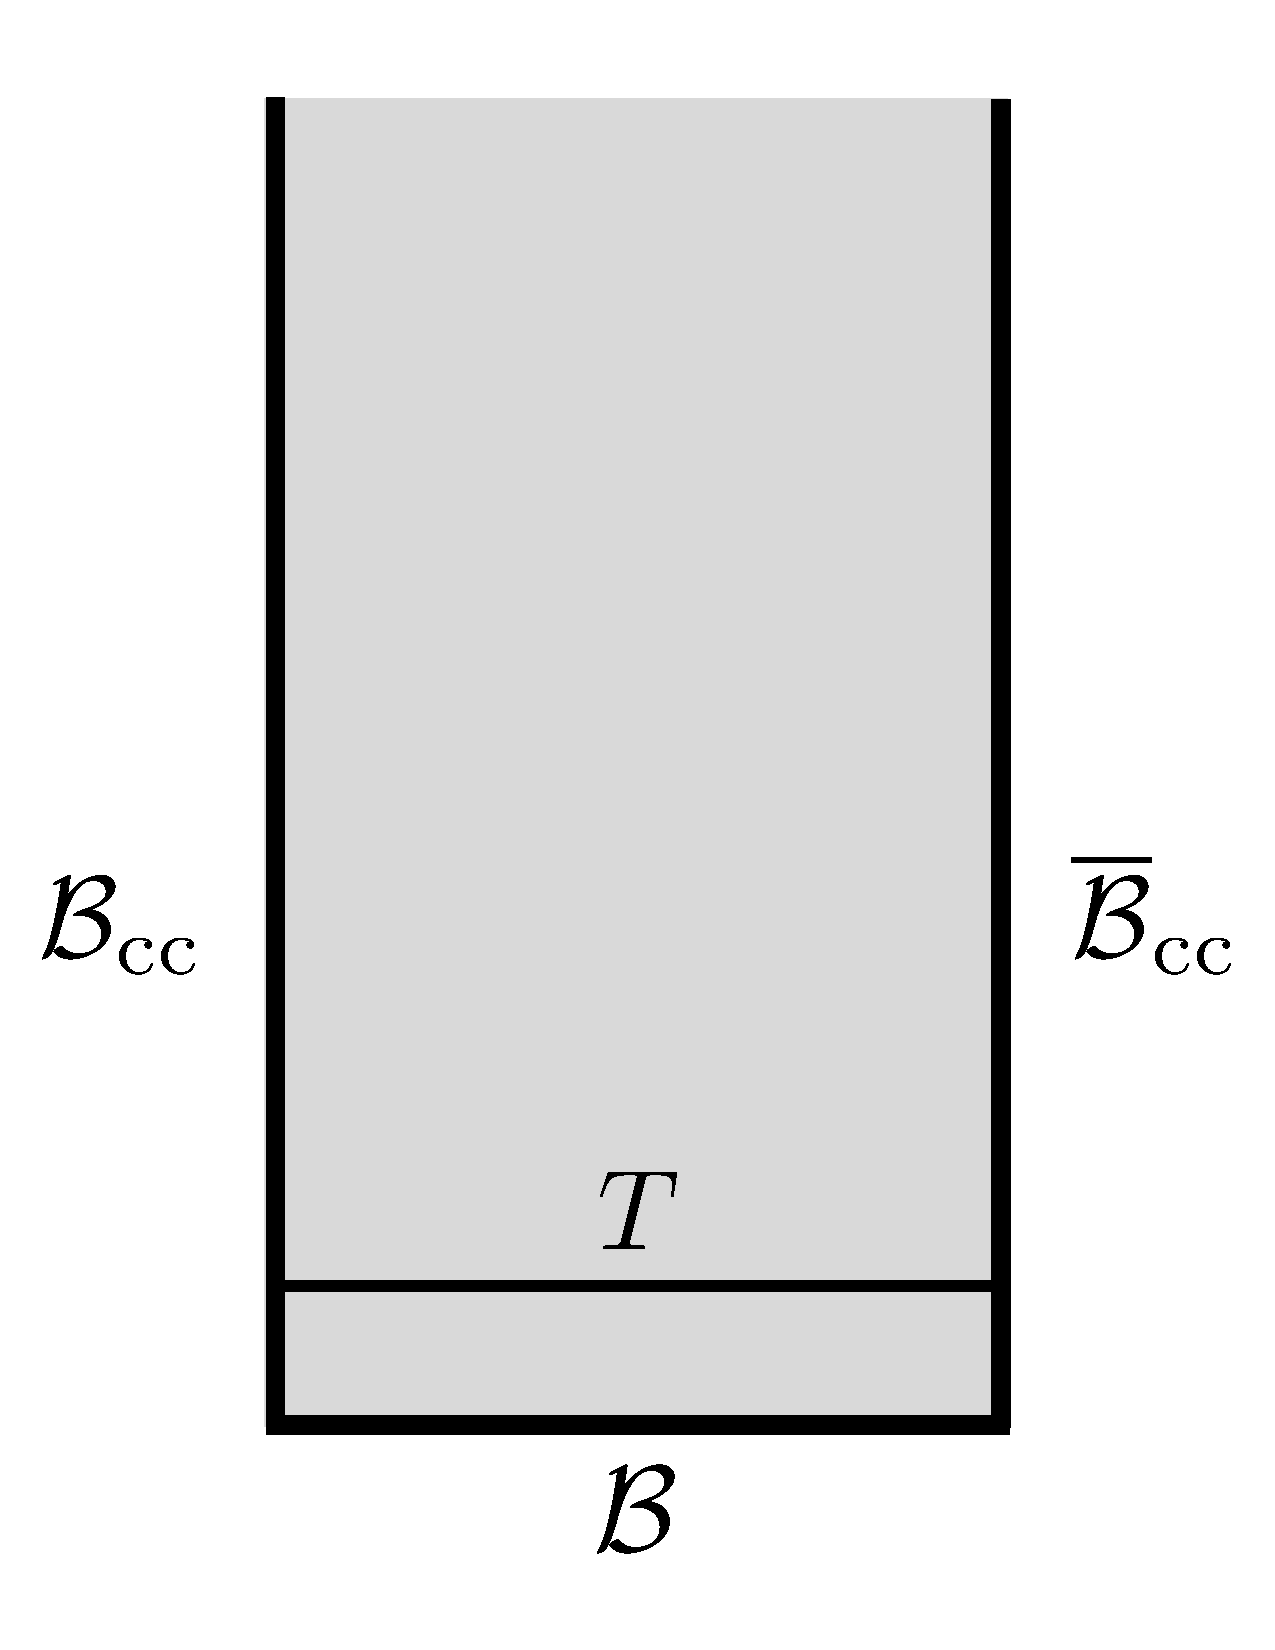
\includegraphics[width=1.7in]{Example8.pdf}
 \end{center}
\caption{\small 一个 BAA 型的 't Hooft 算符 $T$，作用在由 BAA 型膜 $\B$ 生成的态上，并附有适当的手征角。我们可以把 $T$ 与 $\B$ 融合，得到一个新的 BAA 型膜 $T\B$。这涉及我们在图 \ref{example1}(a) 中最初讨论的线算符对膜的作用。此外，我们还须考虑 $T$ 与 $\B$ 的左、右端点或边界处各手征角的复合。  \label{example8}}
\end{figure} 

我们也可以讨论：在用手征代数角描述 't Hooft 算符对膜所生成的态的作用的四维图景中，会出现哪些手征代数要素。在图 \ref{example8} 中，我们勾勒了一个 BAA 型的 't Hooft 算符 $T$，它作用在由同型膜 $\B$ 生成的态上，并带有适当的手征角与反手征角。$T$ 对态的作用可以描述为：把 $T$ 所代表的界面与边界 $\B$ 融合，同时把相应的角分别与 $\B_\cc$ 及 $\bar \B_\cc$ 作复合。在四维中，与图 \ref{example8} 的二维图像不同，'t Hooft 线缺陷与半 BPS 边界之间有明显的差别：前者支撑在一点 $p\in C$ 处，而后者缠绕整个 $C$。所以复合 $T\B$ 在远离 $p$ 处与 $\B$ 重合；它可以描述为用一条线缺陷增广的膜 $\B$。因此，为描述 't Hooft 算符的作用，我们首先应当把本节的讨论推广到允许边界线缺陷在一点 $p\in C$ 处终结于交汇的情形。照例，这一设置将全纯地依赖于 $p$。它之所以只依赖于 $p$，是因为在 $A$-扭化理论中，边界线缺陷本身是一个拓扑 't Hooft 线缺陷的像，因而也是拓扑的。

边界线缺陷 $\ell$ 及其端点的存在，既不影响 $C$ 上其他位置可用的手征代数算符的选取，也不影响它们在远离 $p$ 处满足的 Ward 恒等式。但它影响它们在 $p$ 附近的行为。对每个 $\ell$，可能的端点 $O_{\ell,i}(p)$ 构成一个向量空间，而它们构成 ${\cal V}$ 的一个模 ${\cal V}_\ell$：模结构编码手征代数算符与端点之间的 OPE，并控制在 $p$ 处由 ${\cal V}_\ell$ 的插入所满足的 Ward 恒等式。

当我们把一个端点为 $\alpha_{R,n}(p)$ 的 't Hooft 算符移到半 BPS 边界处时，会产生一条边界缺陷 $\ell$，同时在交汇处产生一个特定的端点 $S_{R,n}(p) \in {\cal V}_\ell$。我们可以预言这类端点的两个一般性质：它们与手征代数 ${\cal V}$ 的 OPE 非奇异，就像与 Hitchin 哈密顿量相关联的 $S_{\cal P}(z)$ 那样；并且它们满足与 $\alpha_{R,n}(p)$ 相同的关于 $p$ 的微分方程，其系数由 $S_{\cal P}(z)$ 控制。这些性质可以立即导出：沿拓扑方向把 't Hooft 线与边界分开，再把 $S_{R,n}(p)$ 变回 $\alpha_{R,n}(p)$ 即可。

同样，中心性保证：以一族算符 $S_{R,n}(p) O_1(z_1) \cdots O_n(z_n)$ 标记的 $A$-模型角，作为 $z_i$ 的函数满足与仅以 $O_1(z_1) \cdots O_n(z_n)$ 标记的角相同的 Ward 恒等式。这就保证了 't Hooft 算符对膜所生成的态的作用是良定义的。

我们以关于辅助 $\varphi F$ 理论中 't Hooft 线描述的几点评论来结束这一一般性讨论。垂直于 $N$ 的 't Hooft 线可以解释为 $\varphi F$ 理论中的单极子局部算符。${\cal P}[\varphi](z)$ 这样的算符同时作为 $\varphi F$ 理论和四维理论中的局部算符出现，因为它们是基本场的多项式，其定义不依赖于路径积分围道的选取。相反，单极子算符这类无序算符的定义，要求修改路径积分所允许的场构型空间，从而影响积分围道的可能选取。这种修改体现为：四维理论中实际存在一条线缺陷，它在 $N$ 中的 $p$ 处终结。这些考虑也适用于 $\partial N$ 处的边界无序算符；它们将表现为四维理论中一条边界线缺陷的端点 $O_{\ell,i}(p)$。

直接分析 $\varphi F$ 理论中可用的单极子算符空间以及它们在边界处的像，将会很有意义。其中的一些工具已在 \cite{Gaiotto:2016wcv} 中发展出来，并在那里应用于 Chern–Simons 理论。它们涉及仿射 Grassmann 流形上的上同调计算，这些计算很可能给出第 \ref{lineq} 节分析的局部版本。我们把这个练习留给热心的读者。\zy{译者按（无外部依据，据原文校勘）：原文此处作 “affine Grassmanian”，系 “affine Grassmannian”（仿射 Grassmann 流形）之误；本译本按后者处理。}


% ch11: 原文 GLDraft_D.tex 行 2441–2842；§7.3–7.7
% 只译散文（标题、正文、图题、脚注）；公式、\label、\ref、\eqref、\cite、图文件名保持不变。

\subsection{从角到态} \label{fcs}

现在考虑一个条带（strip）：两端分别放置 $\B_{\cc}$ 与 $\bar \B_{\cc}$，底边则由另一张膜 $\B$ 设定边界条件（图 \ref{example6}）。在“角”处，我们刚刚描述的构造给出两个手征代数（chiral algebra）$\V$ 与 $\bar \V$。在角上作适当的算符插入后，条带上的路径积分给出一个（可能只作为分布定义的）态
\be\label{chidef}
\chi = \left|O_1(z_1) \cdots O_n(z_n) \bar O_{n+1}(\bar z_{n+1}) \cdots \bar O_{n+\bar n}(\bar z_{n+ \bar n})\right\rangle
\ee
它属于通常的希尔伯特空间 $\H=\Hom(\b\B_\cc,\B_\cc)$。一个重要特例是：两个角上的手征代数 $\V$ 与 $\bar\V$ 互为复共轭；不过我们并不限于这一情形。位于不同角上的算符之间不可能出现 OPE 奇异性，因此 $\bar \B_{\cc}$ 角上的 $\bar O_j(\bar z_j)$ 不影响 $O_i(z_i)$ 的 Ward 恒等式，反之亦然。

我们也可以考虑 $\chi$ 与一个检验态 $\Psi \in {\cal H}$ 的配对。所得内积一般而言可能并不良定义；但只要 $\Psi$ 足够好，它就是良定义的——例如 $\Psi$ 由条带顶端一张具有紧支撑（compact support）的膜按类似方式产生（图 \ref{example6}(c)）。若对任意算符插入的选取该内积都良定义，它就给出 $C$ 上的一族关联函数
\be
\langle \Psi| O_1(z_1) \cdots O_n(z_n) \bar O_{n+1}(\bar z_{n+1}) \cdots \bar O_{n+\bar n}(\bar z_{n+ \bar n}) \rangle
\ee
这些关联函数满足 ${\cal V}$ 与 $\bar {\cal V}$ 的 Ward 恒等式。

用边界线缺陷（boundary line defect）装饰的半 BPS（half-BPS）边界条件会产生更大的一族态
\be
\left|\prod_i O_i(z_i) \prod_j \bar O_{j}(\bar z_{j}) \prod_k O_{\ell_k,k}(p_k) \bar O_{\ell_k,k}(\bar p_k) \right\rangle,
\ee 
其角数据还包含边界线缺陷的端点。

本节余下部分将针对半 BPS 边界条件的几个基本例子，把这些结构具体写出来。

\subsection{Dirichlet 边界条件}\label{Dbc}
四维半 BPS 的 Dirichlet 边界条件把规范联络 $A$ 固定为在边界上为零——更一般地，固定为在边界上取某个指定值——并以超对称的方式延拓到其余场。特别地，六个标量场中有三个满足 Dirichlet 边界条件，另外三个（其中包括二维 $\sigma$-模型的希格斯场 $\phi$）满足 Neumann 边界条件。

从定义在 $\partial M$ 的一部分 $N$ 上的辅助 $\varphi \cF$ 理论来看，半 BPS Dirichlet 边界条件与变形 Neumann 边界条件之间的交汇，由沿 $\partial N$ 加在场 $\cA_{\bar z}$ 上的 Dirichlet 边界条件表示。规范变换被限制为在边界上平凡；否则就不可能指定 $\cA_{\bar z}$ 沿边界的值。对 $\cA_{\bar z}$ 的共轭 $\varphi=\varphi_z\d z$，我们不加任何边界条件。

由于规范变换被约束为沿 $\partial N$ 平凡，$\partial N$ 上（也就是交汇处）的局部算符不必是规范不变的。取而代之，存在一个作用在 $\partial N$ 上算符的整体 $G$ 对称性\footnote{\label{defglobal} 元素 $g\in G$ 给出的整体对称变换，是一个规范变换 $g(x):N\to G$，其在 $\partial N$ 上的限制为常数，$g(x)|_{\partial N}=g$。它保持条件 $\cA_{\bar z}|_{\partial N}=0$，因此是该边界条件下所定义理论的对称性。常数 $g$ 如何在 $N$ 的内部延拓为一个规范变换并不重要：任意两种选取之差是一个在边界上平凡、且对物理可观测量作用平凡的规范变换。}；$\cA$ 的边界值 $a$ 可以解释为该整体 $G$ 对称性的背景联络。在四维设置中，$G$ 对称性作用在整个半 BPS Dirichlet 边界条件上；但在 $A$-扭化中，$N$ 的内点处没有任何局部算符可供它作用。整体对称性只作用在交汇处的算符上。

标量场 $\varphi$ 是交汇处的一个合法局部算符，它等同于辅助 $\varphi \cF$ 理论中的同一算符。在 $A$-扭化理论中，算符 $\varphi_z$ 实际上就是相应于边界 $G$ 对称性的守恒流。导出这一结果的一种方式如下。若在“自由”边界条件下变分作用量 $I_{\varphi\cF}=\int_N \Tr\,\varphi_z F_{t\bar z}\d t \d^2z$，就会发现 $I_{\varphi \cF}$ 的变分含一个边界项 $\int_{\partial N} \Tr\,\varphi_z\delta A_{\bar z}$，因此 Euler–Lagrange 方程中包含边界条件 $\varphi_z|_{\partial N}=0$，而对 $A_{\bar z}$ 不加限制。反之，若希望边界条件为 $A_{\bar z}=a_{\bar z}$（其中 $a$ 是 $C$ 上某个指定的联络），可以在作用量上加一个边界项，使总作用量成为
\be\label{fullact} I'_{\varphi\cF}=I_{\varphi\cF}-\int_{\partial N}\Tr\,\varphi_z(A_{\bar z}-a_{\bar z}).\ee
此时 Euler–Lagrange 方程给出的边界条件是 $(A_{\bar z}-a_{\bar z})|_{\partial N}=0$，对 $\varphi$ 不加约束。但这时流为 $J_z=\partial I'_{\varphi\cF}/\partial a_{\bar z}=\varphi_z$，与断言相符。

如第 \ref{ACP} 节与 \cite{Gaiotto:2017euk} 所解释的，在把这一问题推广到一般 $\Psi$ 的情形时，$J_z$ 是 Kac–Moody 流这一点在经典层面即可看出；但要证明 level 是 $\Psi-h$ 而非 $\Psi$，还需要一个与我们即将描述的类似的三维单圈计算。当 $\Psi=0$ 时，Kac–Moody level 完全来自单圈计算。所需的计算可以借助一个简单的捷径非常容易地完成，这个捷径在任何维数的规范场论中都有类似物。我们把 $\varphi\cF$ 理论放在平板（slab）$I\times C$ 上，其中 $I$ 是区间 $[0,L]$，两端具有相同的 Dirichlet 边界条件。反常总可以由理论的低能极限算出，因此在此情形可以丢掉沿 $I$ 非常数的模式，约化为一个纯二维理论。这等价于取朴素的 $L\to 0$ 极限。所得的二维理论具有作用量
\be\label{belaction}
\int \Tr \, \varphi_z D_{\bar z} \cA_t\ee
它是场为 $\varphi_z$ 与 $\cA_t$（此时只依赖 $z$ 与 $\bar z$，不依赖 $t$）、自旋分别为 1 与 0、取值于伴随表示的玻色型 $\beta \gamma$ 系统。类似的、取值于伴随表示的费米型手征 $bc$ 系统具有反常系数 $2h$，因此玻色型 $\beta\gamma$ 系统的反常为 $-2h$。在平板 $I\times C$ 上的规范场论中，由于体理论没有反常，反常局域在平板的两个边界上。由对称性，一半反常来自平板的一端，另一半来自另一端，故任一端的反常系数为 $-h$。这个 level 取值具有非常特殊的性质，我们马上就会回顾。Kac–Moody level 的取值 $-h$ 常被称为临界 level（critical level），记作 $\kappa_c$。\zy{译者按：临界 level $\kappa_c=-h$ 的特殊性在于 Sugawara 构造 $T(z)=\frac{1}{\kappa+h}S_2(z)$ 的分母为零：通常的应力张量退化，$S_2$ 与所有 Kac–Moody 流的 OPE 变为正则，从而成为中心元。标准处理见 P. Di Francesco, P. Mathieu and D. Sénéchal, \emph{Conformal Field Theory}, Springer, 1997, §15。}

下面来确定 $\varphi\cF$ 规范场论的体局部算符 ${\cal P}[\varphi](z)$ 在 ${\cal V}$ 中的像。朴素地看，像就是 ${\cal P}[J](z)$。然而，由于 $J_z$ 与自身的 OPE 奇异性，这一表达式并不良定义。我们可以用点分裂（point splitting）来正规化它，小心地减去奇异项。这其实是二维共形场论中一个熟悉的练习。

最简单的例子是二次哈密顿量 $\Tr\, \varphi_z^2$ 的像。该算符的正规化版本就是 Sugawara 算符 $S_2(z)$。回忆一下：对一般的 level $\kappa$，Sugawara 算符与应力张量成正比，$T(z) = \frac{1}{\kappa + h} S_2(z)$。特别地，$S_2(z)$ 的 OPE 的奇异部分
\begin{equation}
S_2(z) J(w) \sim (\kappa + h)\frac{J(w)}{(z-w)^2} + (\kappa + h) \frac{D_w J(w)}{z-w} + \cdots
\end{equation}
正比于经临界平移后的 level $\kappa+h$。当 $\kappa=\kappa_c=-h$ 时，$S_2(z)$ 与 Kac–Moody 流的 OPE 非奇异，也就是说它是中心元。这正是我们期望 $\Tr \varphi_z^2$ 在 ${\cal V}$ 中的像所具有的性质，并且在具有相同标度维数的算符中完全刻画了它。因此 $S_2(z)$ 对应二次的 Hitchin 哈密顿量。

更高次哈密顿量的正规化要费力一些，但我们可以援引一个一般定理 \cite{BD}：$G$ 的临界 Kac–Moody 代数的中心由一组中心元 $S_{\P}(z)$ 生成，这些中心元正是 ${\cal P}[J](z)$ 的正规化。作为代数，临界 Kac–Moody 代数的中心同构于朗兰兹对偶群 $G^\vee$ 的 oper 流形 $L_\op$ 上全纯函数的空间。由此我们断定：$S_{\P}(z)$ 就是三维算符 ${\cal P}[\varphi](z)$ 在交汇处的像；而通过 $S$-对偶，这些三维算符又被等同于 $L_\op$ 上全纯函数代数的生成元。

Dirichlet 边界上存在整体 $G$ 对称性，这为全纯-拓扑（holomorphic–topological）BAA 型膜的构造增添了一个要素。如前所述，我们可以把 Dirichlet 边界条件推广：不再把联络的边界值取为零，而取 $C$ 上任意固定的联络 $a$。这样就得到一整族 BAA 型膜 $\mathrm{Dir}(a)$，由背景 $G$ 联络 $a$ 的选取参数化。在 $A$-扭化理论中，系统只依赖 $\B_\cc$ 角上的 $a_{\bar z}$ 与 $\bar \B_\cc$ 角上的 $a_z$。这一依赖分别编码在 $\B_\cc$ 角的全纯流 $J_z$ 与 $\bar \B_\cc$ 角的反全纯流 $\bar J_{\bar z}$ 之中。\zy{译者按（无外部依据）：BAA 是 Kapustin–Witten 对膜型的记法：按复结构 $I,J,K$ 的顺序，该膜依次为 $B$-型、$A$-型、$A$-型，即 $(B,A,A)$ 型；本译本有时也直接写作“型 $(B,A,A)$ 的膜”。参见原文所引 Kapustin–Witten 的工作。}

在交汇处没有局部算符插入时，Dirichlet 边界条件于是定义了一族（分布意义的）态 $\Delta(a) \in \H$。在两个角上插入 Kac–Moody 流 $J_z(z_i)$ 或 $\bar J_{\bar z}(\bar z_j)$，就给出该态对背景联络的泛函导数
\be
\prod_i \frac{\delta}{\delta a_{\bar z}}(z_i) \prod_j \frac{\delta}{\delta a_{ z}}(\bar z_j) \Delta(a)
\ee 
这里对背景联络求泛函导数。
 
全纯与反全纯联络的 Kac–Moody 性质有一个重要推论：这两个流分别守恒。回忆带反常的守恒律：
\begin{align}
D_{\bar z} J_z &= - \frac{\kappa_c}{2 \pi} f_{z \bar z} \cr
D_z J_{\bar z} &= \frac{\kappa_c}{2 \pi} f_{z \bar z}
\end{align}
其中 $f$ 是 $a$ 的曲率。这些式子表明：在 $a$ 的无穷小复化规范变换下，态 $\Delta(a)$ 协变地、但带有反常地变换。精确到 $\lambda$ 的一阶，
\be 
\Delta(a_z + D_z \bar \lambda, a_{\bar z} + D_{\bar z} \lambda )=\left[1+\frac{\kappa_c}{2 \pi} \int_C \Tr\left(\bar \lambda - \lambda \right)f_{z \bar z}  \right] \Delta(a_z,a_{\bar z})
\ee
一个足够好的抽象态 $\Psi \in \H$ 与 $t=0$ 处的 Dirichlet 边界条件配对后，给出一个泛函 $\Psi(a)$；在 $a$ 的无穷小复化规范变换下，它作类似的变换：
\be \label{eq:cogauge}
\Psi(a_z + D_z \bar \lambda, a_{\bar z} + D_{\bar z} \lambda )=\left[1+\frac{\kappa_c}{2 \pi} \int_C \Tr\left(\bar \lambda - \lambda \right)f_{z \bar z}  \right] \Psi(a)
\ee  注意，$\Psi$ 在实规范变换下不变，后者对应 $\lambda=\bar\lambda$ 这一特例。$\Psi(a)$ 对 $a$ 的泛函导数给出临界 Kac–Moody 流与 $a$ 耦合的关联函数。

\subsection{联络与丛}\label{CB}

设 $a$ 是黎曼曲面 $C$ 上的联络，结构群为紧规范群 $G$。考虑一个函数 $\Psi(a)$，它不只在 $G$ 值规范变换下不变，而且在 $G_\C$ 值规范变换下不变；后者在无穷小层面作用为
\be\label{actfor}\delta a_{\bar z}=-D_{\bar z}\lambda, ~~\delta a_z=-D_z\bar\lambda. \ee
这样的函数决定 $\M(G,C)$ 上的一个函数，因为 $\M(G,C)$ 可以看作所有 $G$ 值联络构成的空间对复规范变换群的商。\footnote{这一描述略欠精确，因为要真正把 $\M(G,C)$ 实现为商，还需考虑稳定性方面的因素。但实际上并无困难：只要函数 $\Psi(A)$ 连续且在 $G_\C$ 值规范变换下不变，它就确实下降为 $\M(G,C)$ 上的函数。从所有联络的空间走到 $\M(G,C)$，需要丢掉那些定义不稳定全纯丛的联络，在半稳定者上强加一个等价关系，然后取商。连续且 $G_\C$ 不变的函数 $\Psi(a)$ 必定在该等价关系下不变。无论如何，对 $\lmark^2$ 理论而言，这些考虑都不重要。下一段也有类似的说明。}

反之，给定 $\M(G,C)$ 上的函数 $f$，要在联络空间上定义函数 $\Psi(a)$，只需规定：对给定的 $a$，$\Psi(a)$ 等于 $f$ 在 $\M(G,C)$ 中对应于全纯丛 $E\to C$ 的那一点处的值，而该丛由 $a$ 的 $(0,1)$ 部分决定。这样定义的函数 $\Psi(a)$ 自动在 $G_\C$ 值规范变换下不变。

$\M(G,C)$ 上的函数与 $G_\C$ 不变的联络函数之间的这一对应，可以推广到并不 $G_\C$ 不变、而是带反常地在 $G_\C$ 值规范变换下协变变换的函数 $\Psi(a)$。这些泛函可以等同于 $\M(G,C)$ 上某个线丛的截面。对我们最重要的情形是：$\Psi(a)$ 的全纯与反全纯反常系数均为 $\kappa_c=-h$，如式 (\ref{eq:cogauge}) 所示。此时该线丛实际上就是 $\M(G,C)$ 上的半密度丛，我们稍后会说明这一点。更一般地，若把 $\kappa_c$ 换成别的 level $\kappa$（全纯与反全纯两侧相同），则 $\Psi(a)$ 表示 $|K_{\M(G,C)}|^{\frac{\kappa}{\kappa_c}}$ 的截面。

\begin{yizhu}[译者按：为什么反常系数对应半密度]
$\M(G,C)$ 的辛体积元属于经典辛结构，但不属于 $A$-模型。原文的论证是：若物质泛函的反常为 $2\kappa_c$，则它与 level 为 $-2\kappa_c$ 的 Faddeev–Popov 鬼场系统相乘后总反常为零，BRST 流幂零，被积式与代表的选取无关，因而可在 $\M(G,C)$ 上积分——这就是“密度”。反常减半即得半密度，即 $|K_{\M(G,C)}|^{1/2}$ 的截面；一般 level $\kappa$ 则给出 $|K|^{\kappa/(2\kappa_c)}$（原文作 $\kappa/\kappa_c$，疑为笔误；两者在 $\kappa=\kappa_c$ 时一致）。原文借玻色弦中心荷 $c=26$ 的路径积分作类比，并指出这一对应最早由 Beilinson 与 Drinfeld 给出（见原文所引其著作）。
\end{yizhu}

要说明“以全纯与反全纯反常系数 $\kappa_c$ 变换的函数对应 $\M(G,C)$ 上的半密度”，有许多办法（这最早由 Beilinson 与 Drinfeld \cite{BD} 指出）。我们的做法是先说明：以反常系数 $2\kappa_c$ 变换的函数是 $\M(G,C)$ 上的密度。所谓 $\M(G,C)$ 上的密度，是指这样一种对象：它可以在 $\M(G,C)$ 上自然地积分，而不需要用到 $\M(G,C)$ 的任何结构，只用到它是联络空间对 $G_\C$ 值规范变换群的商这一事实。要判断 $\Psi(a)$ 属于哪一类可在 $\M(G,C)$ 上积分的对象，我们将使用一个与玻色弦路径积分之定义有些类似的构造。

考虑一个带联络 $a$ 的二维 $G$ 规范场论，它与某个物质系统耦合，后者具有 level 为 $(\kappa, \kappa)$ 的全纯与反全纯 Kac–Moody 对称性。由于该理论的路径积分在复化规范变换下形式不变，我们可以期望把路径积分规范固定为 $\M(G,C)$ 上的积分。为此需要一族规范固定条件。我们只需对 $\M(G,C)$ 中的每一点 $m$ 挑一个代表二维联络 $a[m, \bar m] = (a_z[\bar m], a_{\bar z}[m])$，并取规范 $a = a[m, \bar m]$。目标是把对 $a$ 的积分化为对 $m,\bar m$ 的积分。

我们按惯例为这一规范固定引入 Faddeev–Popov 鬼场（ghost）。具体地说，引入与复化规范参数 $\lambda$、$\bar \lambda$ 相应的伴随值鬼场 $c$、$\bar c$，以及与规范固定条件相应的伴随值 1-形式 $(b_z, \bar b_{\bar z})$。鬼场作用量为
\begin{equation}
\int\left( \Tr \,b_z D_{\bar z} c +  \Tr \,b_{\bar z} D_z c\right)\d^2z.
\end{equation}  
该鬼场系统具有全纯与反全纯 Kac–Moody 对称性，level 为 $(2h,2h)=(-2\kappa_c, -2\kappa_c)$。众所周知，BRST 流幂零，当且仅当物质加鬼场的总反常为零，即当且仅当 $\kappa - 2 \kappa_c=0$。

$\M(G,C)$ 上的被积表达式是借助 $b$ 的零模准备好的。若把物质配分函数记作 $\Psi(a)$，则规范固定后的路径积分成为
\begin{equation}
\int_{\M(G,C)} \Psi\left(a[m,\bar m]\right) \left\langle \prod_i \left[\int_C b_z \frac{\partial a_{\bar z}[m]}{\partial m_i} \d m_i \right] \left[\int_C b_{\bar z} \frac{\partial a_{z}[\bar m]}{\partial \bar m_i} \d \bar m_i \right] \right\rangle
\end{equation}   这里我们只是模仿了玻色弦与全纯、反全纯中心荷均为 $c=26$ 的共形场论耦合时路径积分的通常定义。由此可知：level 为 $2 \kappa_c$ 的规范协变泛函对应 $\M(G,C)$ 上的密度。

于是，如 (\ref{eq:cogauge}) 那样 level 为 $\kappa_c$ 的规范协变泛函对应 $\M(G,C)$ 上的半密度。在这一表述下，我们可以把希尔伯特空间的内积显式写出：
\begin{equation}\label{eq:innergauge}
\left( \Psi', \Psi \right) \equiv \int_{\M(G,C)} \overline{\Psi}'\left(a[m,\bar m]\right) \Psi\left(a[m,\bar m]\right) \left\langle \prod_i \left[\int_C b_z \frac{\partial a_{\bar z}[m]}{\partial m_i} \d m_i \right] \left[\int_C b_{\bar z} \frac{\partial a_{z}[\bar m]}{\partial \bar m_i} \d \bar m_i \right] \right\rangle
\end{equation}

现在，把一个（足够好的）态 $\Psi \in \H$ 联系到一个泛函 $\Psi(a)$，有两条途径：其一，把抽象态等同于 $\M(G,C)$ 上的半密度，再把它提升为联络的泛函；其二，把 $\Psi$ 与平移后的 Dirichlet 边界条件 $\mathrm{Dir}(a)$ 所产生的态 $\Delta(a)$ 作缩并。为说明这两种做法等价，可以这样论证。经典地看，BAA 型膜 $\mathrm{Dir}(a)$ 支撑在 $T^*\M(G,C)$ 中由 $a_{\bar z}$ 所定义丛 $E$ 处的纤维上。这是余法拉格朗日子流形的最简单类型，相应的态 $\Delta(a)$ 具有集中于 $E$ 处的 delta 函数支撑。因此配对 $ (\Delta(a), \Psi)$ 无非就是泛函 $\Psi$ 在联络 $a$ 处的取值。

作为最后一个练习，我们可以回到量子 Hitchin 哈密顿量的定义。我们希望导出一个公式，用与 $\Psi$ 相联系的泛函 $\Psi(a)$ 来表达哈密顿量作用于某个 $\Psi$ 后所得的泛函 $[\D_\P(z) \circ \Psi](a)$。考虑一个条带：左边界取 $\B_\cc$ 边界条件，底边取某个初始条件，它与角上的数据一起定义态 $\Psi$。（这一设置已示意于图 \ref{example6}(b)，其中条带底部的膜记作 $\B_F$。）按定义，泛函 $[\D_\P(z) \circ \Psi](a)$ 通过在左边界插入 $\P[\varphi_z]$ 并把它移到条带的左下角来计算。这样做时，$\P[\varphi_z]$ 被转换为手征代数的中心元 $S_{\P}(z)$，即 $J_z$ 及其导数的某个正规化多项式。反过来，$J_z$ 的插入可以换成对 $a_{\bar z}$ 的泛函导数。于是 $[\D_\P(z) \circ \Psi](a)$ 被表示为作用在 $\Psi(a)$ 上的某个微分算子 $\D^{(a)}_\P(z)$。算符 $\D^{(a)}_\P(z)$ 是 $\P\left[\frac{\delta}{\delta a_{\bar z}} \right]$ 的正规化。它把规范协变泛函映为规范协变泛函，恰恰是因为 $S_{\P}(z)$ 是中心元：$S_{\P}(z)$ 的插入不改变流的 Ward 恒等式，因而微分算子 ${\cal D}^{(a)}_{\P}(z)$ 与规范协变性约束 (\ref{eq:cogauge}) 对易。量子 Hitchin 哈密顿量在数学上正是这样定义的 \cite{BD}：它们刻画了临界 Kac–Moody 代数的共形块（conformal block）中插入一个 $S_{\P}(z)$ 的效果。

要用类似方式表述 Hecke 算符，还需讨论 Dirichlet 边界条件上的边界 't Hooft 算符及其在交汇处的端点。在辅助的三维视角下，边界 't Hooft 算符映为边界单极子算符。这类无序算符（disorder operator）的经典模空间已在 \cite{Costello:2020ndc} 的类似设置中讨论过：它与仿射 Grassmann 流形（affine Grassmannian）$\Gr_{G_\C}$ 重合。\zy{译者按：无序算符指插入后会改变场的边界条件或单值的算符，'t Hooft 算符是典型例子，与 Wilson 算符相对。在三维视角下，边界 't Hooft 算符成为边界单极子算符，其经典模空间为仿射 Grassmann 流形 $\Gr_{G_\C}=G_\C((z))/G_\C[[z]]$，这也是 Hecke 修正的参量空间。参见原文所引 Costello 等的讨论。}

存在无序算符时，距边界某个小距离处的规范丛，是联络的边界值所决定的那个固定丛的某个特定 Hecke 修正（Hecke modification）。相应地，为使 $\varphi_z$ 在距边界某距离处非奇异，它在边界处必须有某些指定的极点与零点。这一“裸的”边界单极子构型可以用 $\varphi_z$ 的局部泛函来装点（dress）。

在第 \ref{sec:chiral} 节中我们将讨论手征代数里的“谱流算符（spectral flow operator）”$\Sigma_g$：它们由 $\Gr_{G_\C}$ 中的一点标记，并对 $J_z$ 施加适当版本的约束。谱流算符及其 Kac–Moody 后代可以扮演边界 't Hooft 算符端点的角色。我们将看到存在某些（连续的）谱流算符的线性组合，它们是中心元，因而可以扮演体 't Hooft 算符端点的像 $S_{R,n}(z)$ 的角色。这将使我们能用二维手征代数的语言表述 Hecke 算符。

%We have not found obvious contradictions with these statements, 
%
%In the quantization of $T^*\M(G,C)$, a delta function $\delta_E$ arises as the quantization of the cotangent fiber $T^*_E$ of $T^*\M(G,C)$. This is the simplest example of a conormal Lagrangian manifold. The $A$-model corners consist of polynomials of the fiber variables, mapping to derivatives of $\delta_E$ at $E$. 
%
%For a nice enough bundle $E$, the fiber $T^*_E$ is closed in $\M_H(G,C)$ and thus provides a reasonable support for a BAA brane. 
%We thus expect $\delta_E$ and its derivatives to be good distributional states. This is not always the case, though. There are bundles 
%$E$ for which the fiber $T^*_E$ is not closed in $\M_H(G,C)$ and thus is not a suitable support for a BAA brane. We could attempt to define a BAA brane supported on the closure of $T^*E$ in $\M_H(G,C)$, but polynomials on $T^*_E$ may not extend to holomorphic sections of $K^{\frac12}$ on the closure. As a consequence, whatever distributional states are defined by such a BAA brane will not behave as expected from $\delta_E$ and its derivatives. We conclude that a Dirichlet boundary condition coupled to a connection $a$ associated to such a bundle should give a BAA brane which is not the fiber $T^*_E$ nor its closure. 
%
%There is a potential mechanism for this. Dirichlet boundary conditions in flat space have a non-trivial space of vacua, controlled by solutions of Nahm's equations. The space is roughly identified with the regular nilpotent orbit ${\cal O}$ of the Lie algebra of $G$. Upon twisted compactification on a Riemann surface, the space of vacua does not necessarily disappear. The main difference is that the scalar field whose boundary expectation value  parameterizes ${\cal O}$ becomes the Higgs field. The space of vacua will thus survive classically if the Higgs field can acquire a nilpotent expectation value. This may lead to bubbling phenomena, where the bundle 
%which appears at some distance from the boundary is not the same as the bundle defined by the boundary connection $a$. 
%
%There is a known relation \cite{2017arXiv171010152P,2018arXiv180404881Z} between ``wobbly'' bundles which admit nilpotent Higgs fields and ``shaky'' bundles for which $T^*_E$ is not closed. It would be interesting to see if properties of Dirichlet boundary conditions can provide a novel interpretation of this relation.

%In order to produce distributional states, we need a four-dimensional lift of corners between the $T^*_E$ branes and $B_{\cc}$ boundary conditionc as well. Deformed Neumann boundary conditions have a known supersymmetric two-dimensional junction with Dirichlet boundary conditions \cite{Gaiotto:2017euk}. This junction can be compactified on $C$ to produce a canonical corner in the 2d $A$-model. The two-dimensional junction supports a collection of holomorphic Q-closed local operators, which can be added at points in $C$ to produce a whole collection of 
%$A$-model corners. Based on the work on corner vertex algebras, we expect these operators to define a chiral Kac-Moody algebra at critical level. 
%
%This is very natural. As we will review in Section \ref{sec:chiral}, derivatives along $\M(G,C)$ of a half-density are naturally described in terms of correlation functions of critical Kac-Moody currents. In general, functional analysis on $\M(G,C)$ has a natural 2d CFT interpretation which lifts to a natural four-dimensional interpretation. For example, holomorphic local operators on the deformed Neumann boundary conditions can be brought to the junction along a topological direction. Their image at the junction should have trivial OPE with any junction local operator. Indeed, the chiral Kac-Moody algebra at critical level includes central operators which precisely match the quantum Hitchin Hamiltonians, and are usually employed to define the quantum Hitchin Hamiltonians themselves. We will also discuss an analogous interpretation of the quantum Hecke operators. 

\subsection{Nahm 极点边界条件}\label{nbc}

半 BPS 的 Dirichlet 边界条件可以推广为范围更大的一族 Nahm 极点（Nahm pole）边界条件，由一个嵌入 $\rho:\mathfrak{su}(2)\to\g$ 标记。这类边界条件允许选取一个背景联络 $a_\rho$，其结构群与 $\rho$ 对易。

仿照 \cite{Gaiotto:2017euk} 中 $\Psi \neq 0$ 的结果，我们暂定把这些边界条件相应的手征代数等同于 ${\cal W}^G_{\rho;\kappa}$ 手征代数的临界 level 极限；后者又定义为 level 为 $\kappa$ 的 $G$ Kac–Moody 代数沿 $\rho$ 的 Drinfeld–Sokolov 约化。作为对这一提议的基本检验，我们注意到 ${\cal W}_{\rho;\kappa_c}$ 与临界 Kac–Moody 情形一样具有很大的中心，由适当的 $S_{\cal P}(z)$ 生成。

一个特别有趣的情形是与正则嵌入 $\rho$ 相应的 Nahm 极点。此时手征代数是一个 $W$-代数的经典极限，且完全由中心构成。它由 $S_{\cal P}(z)$ 生成：交汇处的所有局部算符都是变形 Neumann 边界上局部算符的特化。

正则 Nahm 极点相应于一张 BAA 型膜 $\B_N$，它支撑在 Hitchin 纤维化的 Hitchin 截面（Hitchin section）上。该截面是 $\M_H$ 的一个 BAA 型复拉格朗日子流形，但它完全位于 $T^*\M(G,C)$ 之外。若把 Hitchin 哈密顿量的一个本征态 $\Psi$ 纯粹看作 $\M(G,C)$ 上的平方可积半密度，那么计算 $\Psi$ 与 $\B_N$（带适当角）所产生之态的内积似乎毫无意义，因为平方可积半密度的空间来自 $T^*\M(G,C)$ 的量子化，而 $T^*\M(G,C)$ 与 $\B_N$ 的支撑完全不相交。然而，如第 \ref{wkb} 节所讨论的，$\Psi$ 实际上相应于 $\M_H$ 中一张具有紧支撑的膜，因此它与任何膜所产生的态都应有良定义的配对。事实上，在对偶的 $B$-模型中，这一计算是直截了当的。我们将在附录 \ref{bmodel} 末尾回到这一点。

正则 Nahm 极点边界支持边界 't Hooft 线，这些线已在 \cite{Witten:2011zz} 中研究过。它们与体 't Hooft 线自然对应，而且确实就是把体 't Hooft 线搬到边界所得到的像。于是，用边界 't Hooft 算符装饰的 Nahm 极点边界条件给出 BAA 型膜，其支撑是 Hitchin 截面在一族点处的 Hecke 修正。若点的数目足够多，这些 BAA 型膜就是 $T^*\M(G,C)$ 中相当好的子流形。相应的态应在 \cite{T} 的分离变量（separation of variables）分析中起作用。

\subsection{增广 Neumann 边界条件}\label{Enriched}

在 $\M_H(G,C)$ 的二维 $\sigma$-模型中，一个基本的 BAA 型边界条件是与拉格朗日子流形 $\M(G,C)\subset \M_H(G,C)$ 相应的拉格朗日边界条件。用四维语言说，它来自一个 BAA 型的半 BPS 边界条件，其中规范场 $A$ 满足 Neumann 边界条件，而希格斯场 $\phi$ 满足 Dirichlet 边界条件。\footnote{膜 $\B_\cc$ 则来自对 $A$ 的 Neumann 边界条件的一种变形，其意义见脚注 \ref{deformed}；这一变形以不同方式延拓到超多重态的其他分量，并保持另一种对称性（ABA 而非 BAA）。} 我们把该边界条件称为 BAA Neumann。

用 $\varphi\cF$ 理论来说，这不过是由 $\varphi|_{\partial N}=0$ 定义的边界条件，对 $A_{\bar z}|_{\partial N}$ 不加约束。我们在第 \ref{Dbc} 节已说明：对所有场取“自由”变分时，这就是由作用量 $I_{\varphi\cF}$ 的 Euler–Lagrange 方程得到的边界条件。

在此边界条件下，边界上的规范变换不受任何限制。这是自洽的，因为边界条件 $\varphi|_{\partial N}=0$ 是规范不变的。然而，$N$ 的取此边界条件的边界上存在规范反常（gauge anomaly）。反常系数为 $+h$。

看出这一点的一个简便办法，是考虑平板 $N=I\times C$ 上的 $\varphi\cF$ 理论：左端取 $\cA_{\bar z}=0$ 边界条件，右端取 $\varphi_z=0$ 边界条件。这两个边界条件在由元素 $g\in G$ 给出的常数规范变换下不变。在平板左端，常数规范变换被解释为整体对称性。这就给出 $G$ 作为平板上理论整体对称群的一个作用。一端取 $\varphi_z=0$、另一端取 $\cA_{\bar z}=0$ 的这个理论是完全平凡的：在规范变换意义下（模去一个规范变换），唯一的经典解是处处 $\varphi_z=\cA_{\bar z}=0$，而且没有低能激发。所以 $G$ 作用无反常。由于它通过常数规范变换作用，其反常系数等于左端整体对称性的反常系数与右端规范对称性的反常系数之和。我们在第 \ref{Dbc} 节已知：左端整体对称性的反常系数为 $-h$。因此右端的规范对称性必有反常系数 $+h$。

简言之，$\varphi\cF$ 理论中的 $\varphi_z=0$ 边界条件具有反常 $+h$。修补这一反常的一个可能办法，是在交汇处添加反常为 $-h$（即临界 level）的额外自由度。交汇处的幺正自由度无济于事，因为它们的反常系数为正。我们转而可以这样做。BAA Neumann 边界条件可以被“增广”（enrich）：在保持 BAA 型超对称的前提下，往边界上添加三维物质自由度，使它们构成一个具有 $\N=4$ 超对称的三维超共形量子场论（SQFT）。我们把所得的边界条件称为增广 Neumann 边界条件（enriched Neumann boundary condition；需要指明时，称 BAA 型的）。有趣的情形是该 SQFT 具有 $G$ 对称性，并与体 ${\cal N}=4$ 理论的规范场 $A$ 耦合；这是可能的，因为在 Neumann 边界条件下，$A$ 在边界上不受约束。体四维理论的 $A$-扭化会诱导边界三维 SQFT 的 $A$-扭化。扭化后的边界理论可以对交汇处的反常贡献负的量。对我们的应用而言，我们需要三维 SQFT 具有全纯边界条件，且该边界条件支持临界 level $\kappa_c=-h$ 的 $G$ Kac–Moody 代数。\zy{译者按：这里的机制是“以负补正”。$\varphi_z=0$ 边界带反常 $+h$；而三维 SQFT 经 $A$-扭化后，其全纯边界上的手征代数可以带负的反常，恰好抵消前者。最简单的实现是自由超多重态：扭化后其边界路径积分就是辛玻色子的围道积分，而后者的 Kac–Moody level 为负。参见原文所引 Costello 与 Gaiotto 等的论文。}

为此，我们可以采用 \cite{Costello:2018fnz} 中定义的全纯边界条件之一。“增广”的效果是：终结于增广 Neumann 边界的 $\varphi\cF$ 理论的边界条件不再是 $\varphi_z|_{\partial N}=0$；取而代之，$\varphi_z|_{\partial N}$ 等于该 SQFT 边界手征代数的临界 Kac–Moody 流。特别地，$\P[\varphi_z]$ 的像 $S_{\P}(z)$ 等同于由物质的临界 Kac–Moody 流构造的中心元。

最简单的例子是：SQFT 是自由三维超多重态（hypermultiplet）的理论，这些超多重态在 $G$ 的某个辛表示 $R$ 中变换。设 $Z$ 为超多重态中的玻色场。扭化把 $Z$ 的各分量变成旋量，但仍取值于表示 $R$。如 \cite{Gaiotto:2016hvd} 所分析，在适当类型的边界条件下，带边三维流形上扭化超多重态的路径积分是一个具有全纯作用量的二维围道路径积分（contour path integral），属于第 \ref{ACP} 节所述的一般类型。此时全纯作用量为
\begin{equation}
S[Z,\cA] = \int_C \langle Z, \bar \partial_\cA Z \rangle .
\end{equation} 
其中 $\langle \cdot,\cdot \rangle$ 表示 $R$ 上的辛配对，并且我们已计入与复规范场 $\cA$ 的耦合。具有这种作用量的场 $Z$ 有时称为辛玻色子（symplectic boson），它们确实具有负的 Kac–Moody level；更多讨论见第 \ref{sb} 节。最简单的可能是选取使 level 恰为 $-h$ 的 $R$。也可以选取使 level 更负的 $R$，再用放在交汇处的、属于 $G$ 的实表示 $R_f$ 的一些额外二维手征费米子来补足差额。这里我们讨论最简单的可能，并在末尾简要评论一般情形。

现在考虑一个交汇：一侧是支撑 $\varphi\cF$ 理论的变形 Neumann 边界条件，另一侧是由超多重态增广的 BAA Neumann 边界条件。适当的总全纯作用量是 $I_{\varphi\cF}$ 与 $S[Z,\cA]$ 之和：
\be\label{welli}\h I=\int_N \Tr\,\varphi \cF +\int_{C=\partial N}  \langle Z, \bar \partial_\cA Z \rangle .\ee
对 $\cA_{\bar z}$ 的 Euler–Lagrange 方程给出边界条件
\be\label{nell}\varphi_z|_{\partial N}=\mu(Z), \ee
其中 $\mu(Z)$ 是 $G_\C$ 作用在表示 $R$ 上的全纯矩映射（moment map）。这里 $\mu(Z)$ 的各分量（在量子化后）成为物质系统的 Kac–Moody 流；因此这个公式说明了前面那句话：增广之后，适当的边界条件把 $\varphi$ 取为 Kac–Moody 流。

我们还有经典运动方程
\begin{align}
0=\bar\partial_\cA\varphi =\bar\partial_\cA Z.
\end{align}
满足这些条件以及式 (\ref{nell}) 的三元组 $(\cA,\varphi,Z)$ 描述了 $\M_H(G,C)$ 上一张 BAA 型膜。最简单的情形是：给定 $\cA,\varphi$，满足条件的 $Z$ 至多只有一个。若是如此，则那些确实存在相应 $Z$ 的配对 $(\cA,\varphi)$ 在复结构 $I$ 下构成 $\M_H(G,C)$ 的一个复拉格朗日子流形，对应一张 BAA 型膜。这些拉格朗日子流形是余法型的：因为若对某个希格斯配对 $(\cA,\varphi)$ 存在合适的 $Z$，则对 $\varphi$ 作任意标度变换后，同样存在合适的 $Z$。

这些 BAA 型膜的自然量子化是对 $Z$ 的路径积分 \cite{Gaiotto:2016wcv}：
\begin{equation}\label{eq:ZPsi}
\Psi(a) = \int DZ D\bar Z \,e^{\int_C \left[\langle Z, \bar \partial_a Z \rangle -  \langle 
\bar Z, \partial_a \bar Z \rangle\right]}
\end{equation} 
也许还要通过在路径积分中插入一族 $Z$ 与 $\bar Z$ 来修饰，即在路径积分中插入一个非平凡的角 \cite{Costello:2018fnz}。从本文的角度看，这个公式的意义如下。我们把增广 Neumann 膜放在条带底部，扮演图 \ref{example6}(b) 中记作 $\B_x$ 的那张膜的角色。假设条带底部的两个角上没有任何算符插入，则这幅图所定义的、$\H=\Hom(\b\B_\cc,\B_\cc)$ 中的态就是 $\Psi(a)$。这一陈述是合理的，因为 $Z$ 与 $\bar Z$ 场支持临界 level $\kappa_c=-h$ 的流代数，从而这些场的路径积分确实定义 $\M(G,C)$ 上的半密度。

在这一构造中，交汇处的手征代数由三维物质理论边界手征代数中规范不变算符构成的子代数组成；也就是说，它由那些与临界 Kac–Moody 流有平凡 OPE 的、用 $Z$ 及其导数构造的算符组成。可以把上述构造稍作修改：在条带底部的两个角上加入手征与反手征算符；要描述所得的态，只需在式 (\ref{eq:ZPsi}) 中包含相应的因子。

我们将在第 \ref{sec:symp} 节进一步讨论这一构造。

 \begin{figure}
 \begin{center}
   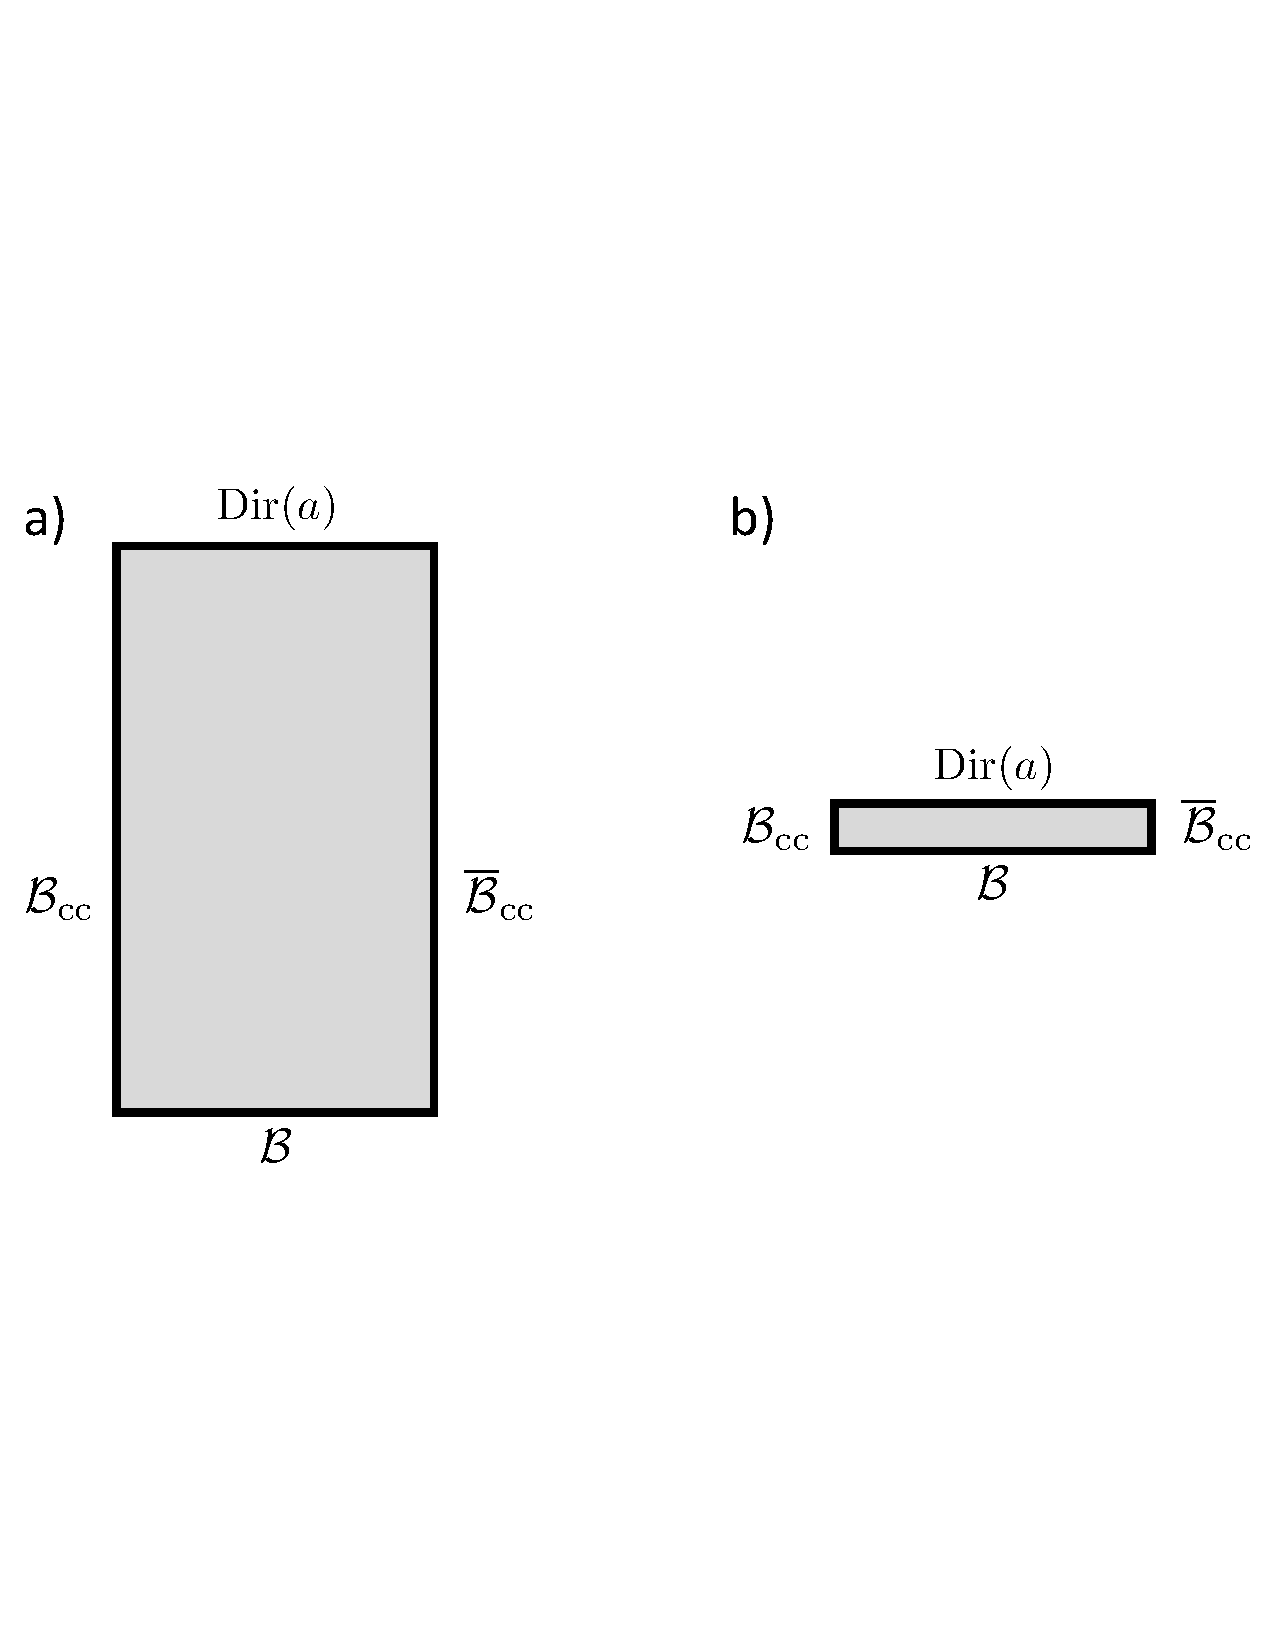
\includegraphics[width=3.2in]{Example9.pdf}
 \end{center}
\caption{\small (a) 一个矩形，底部是增广 Neumann 膜 $\B$，顶部是广义 Dirichlet 膜 $\B'$。(b) 在拓扑场论中，矩形的“高”与“宽”是任意的。在高很小的极限下，问题约化为乘积 $I\times C$ 上纯粹三维的计算。一如既往，$C$ 未画出。\label{example9}}
\end{figure} 

还有一种直接在四维中理解 (\ref{eq:ZPsi}) 的办法。这一替代视角也可以用于更一般的情形：相应的 BAA 型膜带有非平凡的 $\CP$ 丛，或者在交汇处添加了额外的手征费米子。为读出 $\Psi(a)$，我们可以把增广 Neumann 边界所产生的态 $\Psi$ 与 Dirichlet 边界条件 $\mathrm{Dir}(a)$ 所产生的态 $\Delta(a)$ 作缩并。这两个态的内积由如下路径积分表示：在图 \ref{example9}(a) 的矩形上，顶部取 $\mathrm{Dir}(a)$ 边界条件，底部取增广 Neumann 边界条件。在二维拓扑场论中，矩形的“高”与“宽”是任意的。取高远小于宽的极限（图 \ref{example9}(b)）。在此极限下，路径积分约化为 $I\times C$ 上某个三维理论的路径积分。这个三维理论来自沿区间从四维到三维的紧化，区间一端取 Dirichlet 边界条件，另一端取增广 Neumann 边界条件。这一紧化给出简单的答案，因为四维场全都被冻结在其中一个边界上：人们得到的正是当初用来构造增广 Neumann 边界条件的那个三维理论。在我们的例子里，这就是一开始那个自由超多重态的理论，只是现在把整体 $G$ 对称性与作用在 Dirichlet 边界上的 $G$ 对称性等同起来。(\ref{eq:ZPsi}) 的答案就是这个三维理论在 $I\times C $ 上的配分函数，其边界条件产生辛玻色子或其复共轭。于是，即便相应的 BAA 型膜很复杂，我们也可以绕过二维推导而直接使用 (\ref{eq:ZPsi})。在交汇处添加的任何（反）手征费米子都只贡献它们自己的配分函数，即
\begin{equation}\label{eq:ZPsifer}
\Psi(a) = \int DZ D\bar Z D\psi D\bar \psi \,e^{\int_C \left[\langle Z, \bar \partial_a Z \rangle -  \langle 
\bar Z, \partial_a \bar Z \rangle\right]+\left[( \psi, \bar \partial_a \psi ) - ( 
\bar \psi, \partial_a \bar \psi)\right]}
\end{equation} 
只要辛玻色子与费米子的合成 level 为 $-h$，这就表示 $\M(G,C)$ 上的半密度。

本节我们描述了与基本边界条件相联系的态。这一构造很容易推广，用以描述与类似的基本界面（interface）相联系的算符。基本界面的复合可以产生大量 BAA 型边界条件与界面，它们与相应算符的复合相联系。这将允许我们计算（除其他外）$C \times [0,1]$ 上 $A$-扭化三维 ${\cal N}=4$ 规范场论的配分函数，只要线段两端分别取手征与反手征边界条件。关于这一问题以及 $B$-模型中的类似问题，我们将详细分析留待将来工作。\zy{译者按（无外部依据）：本块原文有几处笔误，译文按原意译出、未改原文：§7.7 首段 “of type BAA  in  in which” 多了一个 in；§7.5 中 “correponds” 应为 “corresponds”；§7.7 中 “precisely$-h$” 缺一空格；§7.5 脚注中的 $\lmark^2$ 是源码宏，实际排为 $L^2$。}

% ch12: 原文 GLDraft_D.tex 行 2843–3169；§8
% 只译散文（标题、正文、图题、脚注）；公式、\label、\ref、\eqref、\cite、图文件名保持不变。

\section{Hecke 算符与谱流模}\label{sec:chiral}

\subsection{预备知识}

与增广 Neumann 边界条件（enriched Neumann boundary condition）相联系的 BAA 型膜的量子化，已经为我们提供了波函数的一些例子（\ref{eq:ZPsi}），这些波函数定义为具有手征与反手征临界 Kac--Moody 对称性的二维共形场论的配分函数。本节说明如何直接用二维共形场论的语言，计算量子 Hitchin 哈密顿量与 Hecke 算符作用在这类配分函数上的结果。与此同时，我们也将对第 \ref{wtw} 节中为定义 Hecke 算符而援引的数学结果有更好的理解。

我们已经简要讨论过量子 Hitchin 哈密顿量的二维共形场论解释。临界 Kac--Moody 手征代数有一个很大的中心，它由某些局部算符 $S_{\cal P}(z)$ 生成，这些算符与各流的 OPE 非奇异。关联函数在复化规范变换下的变换方式，由各流的 Ward 恒等式描述。“$S_{\cal P}(z)$ 与各流的 OPE 非奇异”这一断言意味着：插入了这类算符的关联函数只有
\begin{equation}
\langle S_{{\cal P}_1}(z_1) \cdots S_{{\cal P}_n}(z_n) \rangle_a
\end{equation}
满足与配分函数相同的变换性质（\ref{eq:cogauge}）。因此它也定义了 $\M(C,G)$ 上的一个半密度。

此外，$S_{\cal P}(z)$ 由 Kac--Moody 流组装而成，而这些流可以换成关于联络的泛函导数。于是我们可以递推地展开
\begin{equation}
\langle S_{{\cal P}_1}(z_1) \cdots S_{{\cal P}_n}(z_n) \rangle_a = {\cal D}^{(a)}_{\P_1}(z_1 )\langle S_{{\cal P}_2}(z_2) \cdots S_{{\cal P}_n}(z_n) \rangle_a
\end{equation}
而最终结果不依赖于施行递推时所作用算符的次序。因此微分算子 ${\cal D}^{(a)}_{\P_1}(z_1 )$ 彼此交换。

尽管这里谈的是某个二维共形场论的关联函数，但这并非必要：只要给定 $\M(C,G)$ 上的一个半密度，它由联络空间上的规范协变泛函 $\Psi(a)$ 表示，则关于 $a$ 的泛函导数就表现得与 Kac--Moody 流一样。微分算子 ${\cal D}^{(a)}_{\P}(z)$ 以规范协变的方式，表示量子 Hitchin 哈密顿量 ${\cal D}_{\P}(z)$ 对半密度 $\Psi$ 的作用。

在 $C$ 中一点 $p$ 的邻域 $U$ 内作计算时，通常有帮助的做法是为丛选取一个在 $U$ 上为零的代表联络。这总是可能的，因为 $\cA_{\bar z}$ 可以借助取复值的规范变换局部地置零。这相当于把丛在 $U$ 上平凡化，正如我们在第 \ref{affgr} 节讨论一般 Hecke 变换时所做的。于是 Kac--Moody 流在 $U$ 上亚纯，并满足标准形式的 Kac--Moody OPE
\begin{equation}
J^a(z) J^b(w) \sim \frac{\kappa_c \delta^{ab}}{(z-w)^2} + \frac{f^{ab}_d J^d(w)}{z-w}.
\end{equation}

回顾 Kac--Moody 代数 Fourier 模的定义
\begin{equation}
J^a_n \equiv \oint_{|z|=\epsilon} \frac{\d z}{2 \pi \i} z^n J^a(z)
\end{equation}
插入这样一个 Fourier 模，表示 $a_{\bar z}$ 的一个支撑在回路 $|z|=\epsilon$ 上的无穷小形变；或者说，它表示丛的一个形变：借 $U'=U\backslash p$ 中的一个无穷小规范变换，修改 $U$ 上的丛与曲面其余部分上的丛之间的粘合。

若圆盘 $|z|<\epsilon$ 内没有其他算符插入（或只有中心算符插入），则插入了非负 Fourier 模的关联函数为零。相应的无穷小规范变换可以延拓到 $U$ 上，并不改变丛。它们表示 $U$ 上原来那个平凡化的改变。若圆盘内有一个一般的算符插入，则非负模的作用非平凡：插入一个一般的局部算符需要选定丛的某种平凡化，而结果依赖于这一选取。

负的 Fourier 模即使在没有其他算符插入时也可以非平凡地作用，它们表示能够改变丛的无穷小规范变换。负模的反复作用生成 Kac--Moody 代数真空模在 $z=0$ 处的像。算符 $S_{\cal P}(0)$ 以及手征代数中其他中心元，按算符–态对应，就是真空模中被各流的所有非负 Fourier 模消灭的那些向量。例如，Sugawara 向量为
\be
|S_2\rangle \equiv \Tr \,J_{-1} J_{-1} |0 \rangle,
\ee 对其他中心元也有类似的公式。

\subsection{作为中心顶点算子的 Hecke 算符}\label{cvo}

Hecke 积分算符也可以用二维手征代数的方法来分析。我们希望把 Hecke 算符提升为作用在规范协变泛函上的算符，并用与 Kac--Moody 流 OPE 平凡的局部算符的插入，赋予它们二维手征代数的解释。这样的表述立刻保证 Hecke 算符与量子 Hitchin 哈密顿量交换，并且彼此交换。

我们可以逐字照搬第 \ref{affgr} 节中 Hecke 修正的定义。首先，在点 $p$ 的一个小邻域 $U$ 上把丛 $E$ 平凡化。于是可以认为，$E\to C$ 是把 $U$ 上的平凡丛与 $C\backslash p$ 上的丛 $E$ 用平凡粘合映射粘合而成。然后，把粘合映射改为 $z^\m$（其中 $\m$ 是对偶群的一个整权，$z$ 是 $p$ 处的局部参数），由此产生一个新丛 $E'$。丛 $E$ 与 $E'$ 在 $U$ 之外可以用同一个联络描述。描述 $E$ 的联络 $a$ 在 $U$ 上为零；描述 $E'$ 的联络 $a'$ 在 $U$ 之外与 $a$ 重合，而在 $U$ 内可以取为某个特定的参考联络，它支撑在 $U'$ 中的一个环形区域上，并正比于 $\m$。

取表示输入波函数的泛函 $\Psi$，在 $a'$ 上求值。这就给出一个新的泛函 $\Psi_{\m}(a)$。关键在于，$\Psi_\m(a)$ 在复化规范变换下并不协变：新丛 $E'$ 依赖于最初对 $E$ 的平凡化的选取。形式上，$\Psi_\m(a)$ 及其泛函导数可以解释为 Kac--Moody 流在存在“谱流算符”（spectral flow operator）$\Sigma_{\m}(0)$ 时的关联函数。Hecke 算符与 Kac--Moody 代数谱流自同构之间的这一关系，先前已从另一虽不同但相关的角度被注意到，见 \cite{Teschner:2010je} 第 8.5 节。

“谱流”一词指的是 Kac--Moody 代数的某个自同构：
\begin{align}
J^\alpha_n &\to J^{\alpha}_{n+(\m, \alpha)} \cr
J^h_n &\to J^h_n - \m \kappa \delta_{n,0}
\end{align}
其中 $J^\alpha$ 是与根 $\alpha$ 相联系的流，$J^h$ 是 Cartan 流。这恰是 $z^\m$ 规范变换对各流的 Fourier 模的作用。

按定义，谱流模（spectral flow module）是真空模在谱流下的像。特别地，真空向量在谱流下的像被 $n$ 非负的 $J^{\alpha}_{n+(\m, \alpha)}$ 消灭，并且是 $J^h_0$ 的一个具有非平凡本征值的本征向量。\zy{译者按（无外部依据）：谱流并不保持真空，它把整条能谱沿 $J^h_0$ 平移；谱流模因此是真空模在这种平移下的像，其最低权态不再是真空，这正是下文 $|1\rangle$ 满足 $J^0_0|1\rangle=|1\rangle$ 的原因。}相应地，谱流算符 $\Sigma_{\m}(0)$ 是这样的局部算符：在作 $z^\m$ 规范变换之后，它与 Kac--Moody 流的 OPE 变得非奇异。$J^{\alpha}(z)$ 在 $z=0$ 处将有 $(\m, \alpha)$ 阶的极点或零点，而 $J^h(z)$ 将有一个单极点，其留数为\footnote{玻色化（bosonization）为描述 $\Sigma_{\m}$ 提供了一种便利的方式。粗略地说，若把 Cartan 流玻色化为 $J^h = \partial \phi^h$，把其余的流写成顶点算子（vertex operator）$J^\alpha = e^{\frac{\alpha}{\kappa} \cdot \varphi}$，则谱流算符也可以用顶点算子 $\Sigma_{\m} = e^{\m \cdot \varphi}$ 表示。这一表示对某些计算有用，但在一般的 $G_\C$ 规范变换下表现不佳。}$\m\kappa \Sigma_{\m}(0)$。

我们再次强调，泛函 $\Psi_{\m}(a)$ 并不表示 $\M(G,C)$ 上的半密度，因为它依赖于对 $E$ 的平凡化的选取。谱流算符 $\Sigma_{\m}(0)$ 的性质，恰好刻画了规范协变约束（\ref{eq:cogauge}）失效的确切方式。我们的目标是由 $\Sigma_{\m}(0)$ 构造某种局部算符插入，它要是中心的，从而能表示 Hecke 算符对 $\Psi(a)$ 的作用。

在继续一般性讨论之前，先给出 $G=\SO(3)$、最小电荷这一参考例子。基本的谱流自同构为
\begin{equation}
J^\pm_n \to J^{\pm}_{n \pm 1} \qquad \qquad J^0_n \to J^0_n - \delta_{n,0}
\end{equation}
谱流模由一个向量 $|1\rangle$ 生成，它满足
\begin{align}\label{laterref}
J^{\pm}_{n \pm 1} |1\rangle &=0  \qquad \qquad n\geq 0 \cr
J^0_n |1\rangle &=0  \qquad \qquad n> 0 \cr
J^0_0|1\rangle &= |1\rangle.
\end{align}
在这种基本的“电荷 1”谱流算符的情形，我们把 $\Sigma_\m(0)$ 记作 $\Sigma_1(0)$。

依照第 \ref{affgr} 节关于仿射 Grassmann 流形的讨论，我们可以把粘合映射 $z^\m$ 换成同一轨道 $\Gr^\m$ 中的另一个粘合映射 $g$。把 $z^\m$ 换成 $g$ 作同样的构造，便产生一个泛函 $\Psi_{g}(a)$。$\Psi_{g}(a)$ 的泛函导数可以解释为在存在修改后的谱流算符 $\Sigma_{g}(0)$ 时的关联函数。由于平凡化的改变由各流的非负模实现，我们可以把这些模对 $\Sigma_{g}(0)$ 的作用表示成沿 $\Gr^\m$ 的某些微分算子。

应当强调，$\Psi_{g}(a)$ 的定义确实需要选取一个支撑在 $U'=U\backslash p$ 内、实现粘合映射 $g$ 的参考联络。描述同一 $g$ 的不同联络之间差一个复规范变换，因而可能给出 $\Psi_{g}(a)$ 与 $\Sigma_{g}(0)$ 的不同归一化。结果是，$\Psi_{g}(a)$ 与 $\Sigma_{g}(0)$ 实际上是 $\Gr^\m$ 上某个线丛的截面。我们将在第 \ref{fft} 节辨认出这个线丛。\zy{译者按（无外部依据，据原文校勘）：原文此句作 “indentify”，当为 “identify”（辨认、认出）。译文按后者处理。}各流的非负模将作为这个线丛截面上的向量场作用。这正是 Hecke 修正前后半密度丛不相匹配这一事实在手征代数中的体现。

$\Gr^\m$ 上的这个线丛由 Kac--Moody 代数的 level 控制。下一节我们将说明，在临界 level，这个线丛与 $\Gr^\m$ 上的密度丛重合。这意味着，在一个全纯与反全纯 Kac--Moody level 都取临界值的理论中，谱流算符是 $\Gr^\m$ 上的一个密度，可以自然地积分：
 \begin{equation}\label{tendef}
\h\Sigma_\m(0) \equiv \int_{\Gr^\m}\Sigma_{g}(0) |\d g|^2.
 \end{equation}
$\h\Sigma_\m(0)$ 具有恰当的性质，可作为电荷为 $\m$ 的 Hecke 算符，它按第 \ref{wilop} 节的说法对偶于带有最小角 $s_{R}$ 的 Wilson 算符（即用最高权向量构造的波函数所定义的 Wilson 算符）。对 $\Gr^\m$ 的积分推广了式 (\ref{tonf}) 中对 $\bCP^1_x$ 的积分。\zy{上文的临界 level（critical level）指 Kac--Moody 的 level 取 $\kappa_c=-h$，其中 $h$ 是对偶 Coxeter 数；此时 Sugawara 构造退化，手征代数的中心变得很大，故有 $S_{\cal P}(z)$ 这样的中心元。参见 B. Feigin 与 E. Frenkel, ``Affine Kac--Moody algebras at the critical level and Gelfand--Dikii algebras,'' \emph{Int. J. Mod. Phys.} A7 (1992)。}
 
各流的非负模对 $\h\Sigma_\m(0)$ 的作用，可以换成 $\Sigma_{g}(0)$ 沿 $\Gr^\m$ 上相应向量场的 Lie 导数。只要分部积分时不出现边界项（在可能出现单极子冒泡时，这或许需要作技术性的分析），$\h\Sigma_\m(0)$ 就会被 Kac--Moody 代数的非负模消灭，从而是中心的。相应地，平均后的泛函
 \begin{equation} \label{eq:chirhecke}
\int_{\Gr^\m}\Psi_{g}(a)|\d g|^2
 \end{equation}
它由 $\h\Sigma_\m(0)$ 作用于 $\Psi(a)$ 而得，是规范协变的，可以表示电荷为 $\m$ 的主 Hecke 算符（principal Hecke operator）的作用。

我们可以把这套构造直接用于前面 $G=\SO(3)$、最小电荷的示例。可以定义一族以 $\bCP^1$ 参数化的谱流算符 $\Sigma_{1;\mu}(0)$，即把 $\Sigma_1(0)$ 作整体 $\SO(3,\C)$ 旋转。形式上，可以把相应的态写成
\be 
|1;\mu\rangle = e^{\mu J^+_0 }|1\rangle
\ee
把非负 Fourier 模对 $|1;\mu\rangle$ 的作用写成关于 $\mu$ 的微分算子，并验证它们都是全导数，这是不难的。显然有
\be 
J^+_0 |1;\mu\rangle = \partial_\mu e^{\mu J^+_0 }|1\rangle=  \partial_\mu |1;\mu\rangle
\ee
$J^0_0$ 的作用同样不难写出
\be 
J^0_0 |1;\mu\rangle = e^{\mu J^+_0 }(J^0_0 + \mu J^+_0)|1\rangle  =  \partial_\mu \left(\mu |1;\mu\rangle\right)
\ee
计算 $J^-_0$ 的作用只需稍多一点工夫：
\be 
J^-_0 |1;\mu\rangle = e^{\mu J^+_0 }(J^-_0 + 2 \mu J^0_0 + \mu^2 J^+_0)|1\rangle  =  \partial_\mu \left(\mu^2 |1;\mu\rangle\right)
\ee

这就使得下述插入
\be \label{eq:averso}
\int \Sigma_{1;\mu, \bar \mu}(0)|\d \mu|^2
\ee
是中心的，只要分部积分时边界项消失。说明边界项消失的自然办法，是说明 (\ref{eq:averso}) 确实是 $\bCP^1$ 上某个密度的积分。为此，我们需要用第二个坐标片覆盖 $\bCP^1$：从相反的谱流算符 $\Sigma_{-1}(0)$ 出发，把它形变为 $\Sigma_{-1;\mu}(0)$，即
\be 
|-1;\mu\rangle = e^{-\mu^{-1} J^-_0 }|-1\rangle
\ee
非负 Fourier 模对这一族算符的作用，涉及的关于 $\mu$ 的微分算子与作用在 $\mu^2 |1;\mu\rangle$ 上的相同。把反手征模也算进来，我们发现可以一致地认定
\begin{equation}
\Sigma_{-1;\mu}(0) = |\mu|^4 \Sigma_{1;\mu}(0)
\end{equation}
并把它们合并为定义在整个 $\bCP^1$ 上的一个密度 $\Sigma_{1;\mu}(0)$。第 \ref{fft} 节将给出通向这一结果的另一种更一般的途径。

按构造，插入 $\Sigma_{1;\mu}(0)$ 对应于背景联络的一个非常具体的修改 $a \to a'[a;\mu]$。回忆我们所处的规范是：$a$ 在开坐标片 $U$ 内为零，而 $a'[a;0]$ 与 $a$ 相差一个支撑在 $U'$ 中环形区域上的参考联络。插入取指数后的 Fourier 模 $e^{\mu J^+_0}$，又在更宽的一个环形区域上对联络添加一个具体的修改，从而得到 $a'[a;\mu]$。

于是，与 (\ref{eq:averso}) 相应的积分算符 (\ref{eq:chirhecke}) 为
 \begin{equation}\label{eq:chirhesutwo}
\int_{\bCP^1}\Psi(a'[a;\mu])|\d \mu|^2
 \end{equation}
把它与 (\ref{actst}) 比较。那里的 $\Psi(y)$，在这里应写作 $\Psi(a(y))$，其中 $a(x)$ 表示我们为每个丛 $x$ 选定的规范固定代表联络。没有理由认为 $a'[a(x);\mu]$ 已经处于规范固定的形式。需要作一个复化规范变换，才能把它化为修改后的丛 $x_\mu$ 的规范固定形式 $a(x_\mu)$。反常将给出某个重标度因子，我们可以把它写成某个全纯量 $\omega$ 的绝对值：
  \begin{equation} \label{eq:omega}
\Psi(a'[a(x);\mu]) = |\omega(x;\mu)|^2 \Psi(a(x_\mu))
 \end{equation} 
该积分算符变为
  \begin{equation}
\int_{\bCP^1}|\omega(x;\mu)|^2 \Psi(a(x_\mu))|\d \mu|^2
 \end{equation}
我们得到：
  \begin{equation}
F(x,y) = \int_{\bCP^1} |\omega(x;\mu)|\delta(y;x_\mu)|\d \mu|^2
 \end{equation}
其中 $\delta(y;x)$ 是支撑在 $\M \times \M$ 中对角线上的 delta 函数。

(\ref{eq:omega}) 的左端是关于 $x$ 的半密度、关于 $\mu$ 的密度，右端则涉及关于 $y=x_\mu$ 的半密度。于是我们可以把 $\omega(x;\mu)$ 与 $(\ref{conf})$ 中的 $w(\vec x;\mu)$ 视为同一对象。因子 $\omega(x;\mu)$ 编码了 $\Psi$ 在复化规范变换下的反常重标度，因而非零。这使我们能把它等同于 \cite{BD} 引入的全纯因子 $k$。\footnote{我们马上就会看到，$\omega(x;\mu)$ 可以在伴随自由费米子的理论中算出。} 我们把 (\ref{eq:chirhesutwo}) 等同于与 $G^\vee$ 的二维表示相联系的 Hecke 算符 $H_{p=0}$，其角取最小者、对应于 $|k|^2$，如式 (\ref{tonf}) 那样。


\subsection{自由费米子技巧}\label{fft}

上一节我们看到，在具有 Kac--Moody 对称性的共形场论中，算符 $\Sigma_g(0)$（其中 $g$ 是与权为 $\m$ 的 Hecke 变换相联系的规范变换）是 $\Gr^\m$ 上某个线丛的截面。这个线丛由反常决定，故只依赖于共形场论的中心荷 $\kappa$（即 Kac--Moody 的 level）。我们希望就临界 level $\kappa_c=-h$ 的共形场论计算这个线丛，但事实证明，对 level 为 $-\kappa_c=+h$ 的共形场论来计算它格外简单。这将给出我们真正想要的 $\Gr^\m$ 上线丛的逆丛。
 
在 $C$ 上选定一个旋量结构——等价地，选定 $K_C$ 的一个平方根 $K_C^{1/2}$——之后，我们考虑一组自旋为 1/2、取值于规范群伴随表示的手征（Majorana--Weyl）费米子 $\psi^a$。Kac--Moody 流是由正规序（normal ordering）的费米子双线性构造而成，并且由于正规序而具有反常的规范变换。中心荷恰为 $h=-\kappa_c$。\zy{正规序指在算符乘积中把产生算符移到消灭算符右侧、并减去真空期望值；它破坏经典对称性，从而产生此处所说的反常规范变换。参见 P. Di Francesco, P. Mathieu and D. Sénéchal, \emph{Conformal Field Theory} (Springer, 1997)。}

我们断言，伴随自由费米子理论中的谱流算符是 $K^{-1}_{\Gr^\m}$ 的截面。这意味着，临界 level $\kappa_c$ 的共形场论中的谱流算符是它的逆丛、即 $K_{\Gr^\m}$ 的截面。我们将以 $G=\SO(3)$、$\m$ 取最小的情形为例加以说明，并简要指出对其他 $G$ 与 $\m$ 的推广。


选定 $\SO(3)$ 的一个 Cartan 子代数后，我们有手征费米子 $\psi^\pm$ 与 $\psi^0$。$z=0$ 处的基本 Hecke 修正使 $\psi^+$ 在 $z=0$ 处有极点、$\psi^-$ 有零点。这只需在 $z=0$ 处插入一个 $\psi^-$ 便可实现。与点 $(u,v)\in\bCP^1$ 相联系的 Hecke 修正，由 $\psi^-$ 的 $\SO(3,\C)$ 旋转实现，即由 $\psi^-_{(u,v)} \equiv u^2 \psi^-  + 2 u v \psi^0 +  v^2 \psi^+$ 实现。插入 $\psi^-_{(y,v)}(0)$ 会迫使 $\psi^-_{(u,v)}$ 在 $z=0$ 处为零，同时使 $\psi$ 各分量的其他线性组合出现极点。\zy{译者按（无外部依据，据原文校勘）：此句下标作 $(y,v)$，与同句及前文的 $(u,v)$ 不一致，当为 $(u,v)$ 之误；译文照录原文。}


于是在伴随费米子的理论中，我们有 $\Sigma_{1;(u,v)}(0) = \psi^-_{(u,v)}$。它关于 $\bCP^1=\Gr^\m$ 的齐次坐标是二次的，因此是 $\O(2) = K_{\Gr^\m}^{-1}$ 的整体截面，与断言相符。于是在临界 level，本例中的谱流算符是 $K_{\Gr^\m}$ 的截面；这一事实已在第 \ref{cvo} 节中用到。

\begin{yizhu}[译者按（无外部依据，据原文梳理）：临界 level 与自由费米子技巧]
本节的论证可概括为一次“取逆”。临界 level 时手征代数的中心很大，谱流算符的归一化只由反常决定，因此它应是 $\Gr^\m$ 上某个线丛的截面，而该线丛只依赖中心荷。直接算 $\kappa_c=-h$ 并不方便，但伴随自由费米子系统的 level 恰为 $-\kappa_c=h$：其流由正规序双线性构造，反常可以显式算出，于是其谱流算符是 $K^{-1}_{\Gr^\m}$ 的截面；取逆便得到临界 level 的答案：线丛 $K_{\Gr^\m}$（全纯典范丛）。这正是把 Hecke 算符写成 $\Gr^\m$ 上积分的原因。
\end{yizhu}


对一般的规范群与电荷，参考 Hecke 修正使以根 $\alpha$ 标记的费米子在 $z=0$ 处多出 $(\lambda, \alpha)$ 阶的极点或零点。这由一个非常简单的顶点算子实现：
\begin{equation}\label{opspin}
\prod_{\alpha | (\lambda, \alpha)<0} \prod_{n_\alpha =0}^{-(\lambda, \alpha)-1}\partial_z^{n_{\alpha}}\psi^{\alpha}
\end{equation}
不难看出，这个乘积按 $K_{\Gr^\m}^{-1}$ 的截面变换：乘积中每个费米子导数，对应一个在 $\Sigma_\m$ 上非平凡地作用的非负 Fourier 模 $J_{n_\alpha}^\alpha$；这些模给出 $\Gr^\m$ 切空间的一组基。

这一计算可以表述为：比较 Hecke 修正前后作用在 $\psi$ 上的 Dirac 算符的 Pfaffian。\cite{BD} 对这一 Pfaffian 作了详细分析。

由于规范反常，算符 $\Sigma_{g}(z,\bar z)$ 并不是 $z$ 的真正函数。事实上，即使把局部坐标重标度 $z \to \lambda z$，也会把奇异规范变换从 $z^\m$ 变为 $(\lambda z)^\m$，从而招致 Cartan 零模 $\m \cdot J_0$ 作用在谱流算符上，产生一个正比于 $(\m,\m)$ 的非平凡标度维数（scaling dimension）。借助自由费米子技巧，可以研究这种对 $z$ 的反常依赖。例如，对 $\SO(3)$ 与最小的 $\m$，我们插入一个 $\psi^-$，它表现为 $K_C^{1/2}$ 的截面。相应地，在临界 level，谱流算符是 $K_C^{-1/2}\otimes \bar K_C^{-1/2}=|K_C|^{-1}$ 的截面。对平均后的 Hecke 算符 $\h\Sigma_\m(0)$ 而言这仍然成立，因为在本例中 $\Gr^\m=\bCP^1$ 上的坐标标度维数为 $0$，故测度 $\d \mu$ 对标度维数没有贡献。$\h\Sigma_\m(0)$ 是 $|K_C|^{-1}$ 的截面这一点，可由 $S$-对偶预期。这与用来定义对偶 Wilson 算符（第 \ref{wilop} 节）的全纯与反全纯截面 $s$ 与 $\bar s$ 分别是 $K_C^{-1/2}$ 与 $\bar K_C^{-1/2}$ 的截面这一事实相符。

对一般的群与表示，把 $\h\Sigma_\m(0)$ 的标度维数与相应 Wilson 算符的行为匹配起来要更微妙一些。费米子插入的标度维数按电荷的二次方增长，而 $\Gr^\m$ 上测度 $\d\mu$ 的负标度维数也按二次方增长。费米子上的导数与测度的标度维数之间有很好的抵消，使得 $\h\Sigma_\m$ 的标度维数是 $\m$ 的一次函数。对偶 Wilson 算符的标度维数已在第 \ref{wilop} 节中描述过。





\subsection{积分–微分 Hecke 算符与 oper 微分方程}\label{opde}

在第 \ref{lineq} 节中，除了积分核以 delta 函数的形式支撑在 Hecke 对应上的积分型 Hecke 算符之外，我们还考虑了积分–微分型 Hecke 算符，其积分核是 delta 函数的导数。构造这类更一般的 Hecke 算符的自然途径，是考虑插入 $\Sigma_{g}$ 的 Kac--Moody 后代（descendant），它们表示在 Hecke 修正所在位置附近的邻域内取泛函导数 $\frac{\delta}{\delta a}$。我们可以只限于由 Kac--Moody 流负模作用所得的后代，因为非负模可以换成关于 $g$ 的导数，而后者在分部积分时会被积掉。

非负模作用在 $\Sigma_{g}$ 的某个后代上，将给出其他后代的 $g$ 导数的某个线性组合。我们需要后代的某种依赖于 $g$ 的组合，使它们按 $\mathrm{Gr}^\m$ 上密度的方式变换，并且使非负 Kac--Moody 模的作用给出关于 $g$ 的全导数。可以给出一个简单的例子：$\partial_z \h\Sigma_\m(z, \bar z)$。事实上，基本谱流算符 $\Sigma_\m(z)$ 的 $z$ 导数恰与 Cartan Kac--Moody 后代重合：
\begin{equation}\label{firstone} \partial_z \Sigma_\m(z)= \frac{1}{2 \pi \i} \oint \frac{\d w}{w-z} \m \cdot J (w) \Sigma_\m(z, \bar z)\equiv  \m \cdot J_{-1} \circ \Sigma_\m(z, \bar z). \end{equation}
为说明这一关系，回忆在关联函数中插入 $\Sigma_\m(z)$ 表示在 $z$ 的邻域 $U$ 内对背景联络作一个具体的修改。随着 $z$ 变动，被修改的联络也变动。这一变动支撑在环形区域 $U'$ 内，可以用一个流的插入（该流与背景联络的变分相缩并）来描述。整个比较都在由 $\m$ 确定的规范群 $\U(1)$ 子群内进行。作为一个小的捷径，我们可以在它们所实现的丛修正这一层面上，比较 $z$ 导数的效果与积分流插入的效果。若 $\Sigma_\m(z)$ 在 $U'$ 上实现规范变换 $g(w) = (w-z)^\m$，则 $z$ 导数 $\partial_z \Sigma_\m(z)$ 实现 $\partial_z  (w-z)^\m = \frac{\m}{z-w} (w-z)^\m$。其中 $\frac{\m}{z-w}$ 部分对应于 $\m \cdot J_{-1}$ Fourier 模所产生的规范变换，而 $(w-z)^\m$ 再次表示 $\Sigma_\m(z)$。由于我们是在丛修正而非联络的层面上工作，可能会漏掉反常引起的效应。在自由费米子理论中作一个简单的检验即可排除这一点。\footnote{对 $\Sigma_\m(z)$ 的玻色化描述，也是验证这一计算的有效办法。}

把这一关系代入 $\h\Sigma_\m(z, \bar z)$ 的定义，我们发现 $\partial_z \h\Sigma_\m(z, \bar z)$ 可以写成 $\Sigma_{g}(z, \bar z)$ 的某个特定 Kac--Moody 后代在 $\Gr^\m$ 上的积分。

产生这类良定义的积分–微分算子的另一种自然途径，是用 Sugawara 向量或其他中心元的模来取 $\h\Sigma_\m$ 的后代。所得的局部算符显然是规范不变的。我们预期，$\Sigma_{g}(z, \bar z)$ 的 Kac--Moody 后代中那些在 $\mathrm{Gr}^\m$ 上为全导数的 $g$ 依赖组合的分类，将与 't Hooft 线端点 $\alpha_{R_\m,n}$ 的相应分类一致。

%This kind of calculation offers a way to prove the oper-like differential equations which we expect to be satisfied by Hecke operators. For example, for $\SO(3)$ and minimal $\m$, which we denote as $\m=1$, we have 
%\begin{align}\label{useform}
%\partial \Sigma_1 &= J_{-1}^0 \Sigma_1 \cr
%\partial^2 \Sigma_1 &= (J_{-2}^0+ J^0_{-1} J^0_{-1}) \Sigma_1 \cr
%S_{-2} \circ \Sigma_1 &= (J_{-2}^0+ J^0_{-1} J^0_{-1} + J^-_{-2} J^+_0) \Sigma_1
%\end{align}
%so that $\partial^2 \Sigma_1 - S_{-2} \circ \Sigma_1$ is proportional to a total derivative $ J^-_{-2} \partial_\mu \Sigma_1$. (The second equation in eqn.
%(\ref{useform}) is just the derivative of the first one, which is eqn. (\ref{firstone}). The last one follows from eqn. (\ref{laterref}) and the definition of $S_{-2}$.)  Thus the averaged spectral flow operator $\h\Sigma_1$ is annihilated by $\partial_z^2 - S_2(z)$, as expected.
%


\subsection{Wakimoto 实现}
这里我们将借助临界 level 的 Wakimoto 实现，给出 $\Sigma_1$ 诸性质的另一种推导。作为额外的收获，我们还将以另一种方式重新得到 oper 微分方程。

临界 level 的 Wakimoto 实现把 Kac--Moody 流表示为 $\bCP^1$ 上扭化 $\beta\gamma$ 系统的对称流：
\begin{align}\label{waki}
J^+ &= \beta \cr
J^0 &= - \beta \gamma + \partial \alpha \cr
J^- &= -\beta \gamma^2 - 2 \partial \gamma + \partial \alpha \gamma \cr
\end{align}
其中 $\alpha$ 是局部定义的全纯函数。Sugawara 向量简化为 Miura 形式 $S_2 = (\partial\alpha)^2 + \partial^2 \alpha$，从而显然是一个恒等算符的倍数，与各流的 OPE 平凡。

谱流自同构自然地延拓到 $\beta\gamma$ 系统，使得谱流算符给 $\gamma$ 一个零点、给 $\beta$ 一个极点。起这种作用的算符通常记作 $\delta(\gamma)$。与由式 (\ref{firstone}) 得到的 $\partial \Sigma_1$ 的预期形式相比较，可得
\begin{equation}
\Sigma_1 = e^{\alpha+ \bar \alpha} \delta(\gamma)\delta(\bar \gamma).
\end{equation}
指数前的因子提供了 $J^0_{-1} \circ \Sigma_1$ 中的 $\partial \alpha$ 部分。

对这一表达式作 $\SO(3,\C)$ 旋转，给出
\begin{equation}
\Sigma_1(z;\mu) = e^{\alpha+ \bar \alpha} \delta(\gamma -\mu)\delta(\bar \gamma- \bar \mu).
\end{equation}
其中 $\mu$ 是 $\bCP^1$ 上的非齐次坐标。对 $\mu$ 的积分很容易算出，结果为
\begin{equation}
\h\Sigma_1(z) = e^{\alpha+ \bar \alpha} .
\end{equation}
这是恒等算符的一个倍数，因而被各流的所有非负模消灭。此外，oper 微分方程显然成立：$\partial_z^2 \h\Sigma_1(z) = S_2(z)\h\Sigma_1(z)$。

我们预期这一模式对所有的 $G$ 与 $\m$ 都成立。临界 Wakimoto 实现给出的中心元，具有由取值于 Cartan 的 $\alpha$ 构造的 Miura oper 的形式。谱流算符将具有 $\beta \gamma$ 系统的谱流算符与 $\alpha$ 的某个函数相结合的形式。平均后的谱流算符将给出 $\beta \gamma$ 系统恒等算符的倍数，再乘以 $\alpha$ 的某些函数，这些函数给出 oper 微分方程解的 Miura 表达式。


% ch13: 原文 GLDraft_D.tex 行 3170–3425；§9 + 致谢
% 只译散文（标题、正文、图题、脚注）；公式、\label、\ref、\eqref、\cite、图文件名保持不变。

\section{来自辛玻色子的波函数} \label{sec:symp}

\subsection{辛玻色子的基础}\label{sb}
如我们在第 \ref{Enriched} 节所讨论的，由三维超多重态增广的 Neumann 边界条件所产生的态，可由一个路径积分描述
\begin{equation}
\Psi[a] = \int DZ D\bar Z\, e^{\int_C \left[\langle Z, \bar \partial_a Z \rangle -  \langle 
\bar Z, \partial_a \bar Z \rangle\right]}
\end{equation} 
这是{\it 辛玻色子}（symplectic bosons）路径积分的非手征版本。手征辛玻色子是手征费米子的 Grassmann 偶类比物。它们是 $\beta \gamma$ 系统的一个特例，其中 $\beta$ 与 $\gamma$ 的共形维数都被取为 $1/2$。\zy{译者按：$\beta\gamma$ 系统是共形维数 $(\lambda,1-\lambda)$ 的自由玻色鬼场；取 $\lambda=1/2$ 时两个场都是自旋 $1/2$ 的玻色场，其 OPE 因辛形式反对称而与费米子相似，统计却是玻色。标准处理见 J. Polchinski, \emph{String Theory}, Vol.~1 (1998) 第 2 章；D. Friedan, E. Martinec, S. Shenker, \emph{Nucl.\ Phys.} B271 (1986) 93。}

具体地说，手征辛玻色子是一组 $2 n$ 个二维自旋 $1/2$ 的手征玻色场 $Z^a$，其作用量为 
\begin{equation}
\int_{C}\left( \omega_{ab} Z^a \bar\partial Z^b + {\cal A}_{ab} Z^a Z^b\right)
\end{equation}
其中 $\omega_{ab}$ 是常值辛形式，我们还加入了与一个 $(0,1)$ 型背景联络 ${\cal A}_{ab}$ 的耦合，该联络在黎曼曲面 $C$ 上定义一个 $\Sp(2n)$ 丛。\footnote{由于辛玻色子是旋量，我们严格说来并不需要分别定义一个旋量结构与一个 $\Sp(2n)$ 丛。我们改为可以指定一个 $\Spin\cdot \Sp(2n)$ 丛，这一概念与第 \ref{toposubt} 节的 $\Spin\cdot \SU(2)$ 丛完全类似。} 本节除非另有说明，我们采用 Einstein 求和约定。 
 
 与手征费米子的类比并不完全。手征费米子是定义良好的二维 (spin)CFT。
手征辛玻色子则有轻微的反常。反常表现为手征配分函数的一个符号不确定性
\begin{equation}
\int DZ \,e^{\int_{C}\left( \omega_{ab} Z^a \bar\partial Z^b + {\cal A}_{ab} Z^a Z^b\right)} = \frac{1}{\sqrt{\det \bar \partial_{\cal A} }}
\end{equation}
其中我们把作用在 $K_C^{1/2} \otimes E$ 的截面上的 $\bar \partial$ 算子记作 $\bar \partial_{\cal A}$，而 $E$ 是附属于该 $\Sp(2n)$ 丛的秩 $2n$ 丛。\footnote{注意，一般而言 $\bar \partial_{\cal A}$ 没有零模，泛函行列式是定义良好的。对于出现零模的特殊 $\Sp(2n)$ 丛选取，配分函数发散。} 
不过，非手征配分函数
\begin{equation}
\int DZ D\bar Z\, e^{\int_C \left[\langle Z, \bar \partial_A Z \rangle -  \langle 
\bar Z, \partial_A \bar Z \rangle\right]} =  \frac{1}{|\det \bar \partial_{\cal A} |}
\end{equation}
是无歧义的：它可以沿循环 $\bar Z{}^a = (Z^a)^*$ 作真正的路径积分来定义（也就是说，该积分循环由如下要求给出：$\bar Z{}^a$ 是 $Z^a$ 的复共轭）。\zy{译者按（无外部依据）：原文此句作 “by an actual the path integral”，多一冠词 the；§9.2 又有 “the the kinetic operator” 重复 the；§9.4 开头列举三个谱流算符时，$\Sigma'$ 与 $\Sigma''$ 的 $\bar\mu$ 缺撇（其下分项中则各自带撇）。以上均为原文笔误，译文照原文处理，未径改。}

我们在此记下算子乘积展开（OPE）
\begin{equation}
Z^a(z) Z^b(w) \sim \frac{\omega^{ab}}{z-w},
\end{equation}
其中 $\omega^{ab}$ 是辛形式的逆。相应的模代数为 
\begin{equation}
[Z^a_m, Z^b_n] = \omega^{ab} \delta_{n+m,0}.
\end{equation}
由于自旋为半整数，在 Neveu–Schwarz 扇区中——特别是在真空模中——模指标 $n$、$m$ 为半整数。真空满足 
\begin{equation}
Z^a_n |0\rangle =0 \qquad \qquad n>0.
\end{equation}
而模指标在 Ramond 扇区模中为整数，我们将在第 \ref{sec:Ramond} 节讨论这些模。

作用量对 $\Sp(2n)$ 联络 ${\cal A}$ 的变分给出 level 为 $- \frac12$ 的 Kac–Moody 流
\begin{equation}
J^{ab} = \frac12 :Z^a Z^b:
\end{equation}
分数 level 是手征理论整体反常的又一表现。\footnote{$J^{ab}$ 流实际上生成 $\widehat{\mathfrak{sp}}(2n)_{-\frac12}$ 手征代数的一个商：流的双线性型的某些线性组合以及流的导数会消失。辛玻色子真空模中 level $2$ 后代的数目，小于 Kac–Moody 真空模中 level $2$ 后代的数目。} 非手征理论的配分函数定义了 $\Sp(2n,\C)$ 丛空间上一个丛 $|{\cal L}|$ 的定义良好的截面，其中 ${\cal L}$ 是对应于 Kac–Moody level $-1$ 的线丛。 

一旦我们特殊化到四维理论的规范群 $G \subset \Sp(2n)$，就会得到 level 未必临界的 $G$ 流。这标志着一种规范反常，它阻碍变形 Neumann 边界条件与增广 Neumann 边界条件之间存在二维交汇。若 level 比临界 level 更负，我们可以尝试用某个辅助二维系统（例如一组自由费米子）来抵消该反常。在下文即将讨论的例子中，反常从一开始就不存在。

\subsection{三基本例子}\label{tri}

现在我们特殊化到 $n=4$，并集中于 $\Sp(8)$ 的一个子群 $G\equiv \SL(2) \times \SL(2)\times \SL(2)$。
换言之，我们把 $\mathbb{C}^8$ 与 $\mathbb{C}^2 \otimes\mathbb{C}^2 \otimes\mathbb{C}^2$ 等同起来，
并把理论耦合到 $\SL(2) \times \SL(2)\times \SL(2)$ 的联络 $a$。

这给出一些增广 Neumann 边界条件，人们猜测它们与一个三对角界面（tri-diagonal interface）$S$-对偶，后者是支撑在 $\M_H \times \M_H \times \M_H$ 的对角线上、带有平凡 $\CP$ 丛的 BBB 膜 \cite{Gaiotto:2016hvd,Benini:2010uu}。\footnote{这一 $S$-对偶陈述可以推广到其他 $G$，或推广到三个以上副本之间的对角界面。相应的增广 Neumann 边界条件使用 \cite{Benini:2010uu} 中定义的理论。这些理论的边界手征代数已由 Arakawa 的工作 \cite{Arakawa:2018egx} 得知，它们具有临界 level 的 $G$ 流。相应的态将是由 Arakawa 的手征代数构造的非手征二维共形场论的配分函数，而后者目前尚不清楚。} 这一 $S$-对偶等同的基本推论是：由配分函数产生的态 $\Psi[a]$ 应当把三份 $\SL(2)$ Hitchin 哈密顿量与量子 Hecke 算符的作用交织起来。本节余下部分的目标就是证实这一点。
 
我们把辛玻色子场记作 $Z^{\alpha \beta \gamma}(z)$，把辛形式记作
$\epsilon_{\alpha \alpha'}\epsilon_{\beta \beta'}\epsilon_{\gamma \gamma'}$。我们得到三份
$\widehat{\mathfrak{sl}}(2)_{-2}$ Kac–Moody 流，例如
\begin{equation}
J^{\alpha \alpha'} =\frac12 \epsilon_{\beta \beta'}\epsilon_{\gamma \gamma'} :Z^{\alpha \beta \gamma}Z^{\alpha' \beta' \gamma'}:
\end{equation}
我们把这三组流简单地记作 $J$、$J'$、$J''$，在可能时省略指标。 

关键在于，这些流具有临界 level。相应地，Sugawara 向量是中心元。一个值得注意的观察是：此处三个 Sugawara 向量实际上彼此重合：
\begin{equation} \label{eq:sugathree}
:JJ: = :J'J': = :J'' J'':
\end{equation}
 由于三个 Sugawara 向量重合，Sugawara 向量的关联函数也彼此重合。后者由 $\mathfrak{sl}(2)$ 量子 Hitchin 哈密顿量作用在配分函数 $\Psi(a)$ 上得到，而 $\Psi(a)$ 被视为 $\M\times \M \times \M$ 上的半密度。 

\begin{yizhu}[译者按：临界 level 与中心元]
仿射 Kac–Moody 代数 $\hat{\mathfrak g}_k$ 的临界 level 为 $k=-h^\vee$，其中 $h^\vee$ 是对偶 Coxeter 数。对 $\mathfrak{sl}(2)$，$h^\vee=2$，故文中 $\widehat{\mathfrak{sl}}(2)_{-2}$ 恰在临界 level；而对 $\mathfrak{sp}(2n)$，$h^\vee=n+1$，所以 §9.1 中 level $-1/2$ 的流远非临界——这正是原文说 $G$ 流的 level “未必临界”、从而可能出现规范反常的原因。临界 level 上 Segal–Sugawara 构造退化：由流双线性型构成的 $:JJ:$ 不再给出 Virasoro 张量，而与所有模式对易、成为中心元；临界 level 真空模具有很大的中心，其结构由 Feigin 与 Frenkel 系统研究（B. Feigin, E. Frenkel, ``Affine Kac--Moody algebras at the critical level and Gelfand--Dikii algebras,'' \emph{Int.\ J.\ Mod.\ Phys.} A7 (1992), Suppl.~1A, 197）。这也说明原文强调“三个 Sugawara 向量重合”为何是有内容的陈述：三者都是中心元，才可以这样逐点比较。
\end{yizhu}

具体地说，辛玻色子 $Z$ 的动能算子是作用在丛 $E \otimes E' \otimes E'' \otimes K_C^{\frac12}$ 上的 $\bar \partial_{a}$ 算子。
配分函数为： 
\begin{equation}\label{sqr}
\Psi(a) = \frac{1}{|\det \bar \partial_a|}.
\end{equation}  
这样，我们就给出了如下交织性质的一个手征代数推导
\begin{equation}
\boxed{H_i \Psi = H'_i \Psi = H''_i \Psi}
\end{equation}
其中 $H_i$ 取遍作用在三份 $\SL(2)$ 丛空间上的 $\mathfrak{sl}(2)$ 量子 Hitchin 哈密顿量。
类似地
\begin{equation}
\boxed{\bar H_i \Psi = \bar H'_i \Psi = \bar H''_i \Psi}
\end{equation}
对共轭的量子 Hitchin 哈密顿量成立，它们作为反全纯微分算子作用在 $\SL(2)$ 丛空间上。
这些关系与 B-模型一侧对三对角界面的预期相符。 
我们的下一个目标是证明 Hecke 算符的类似交织关系。 

为简单起见，我们将使用 $\SO(3)$ 的最小荷 Hecke 算符，尽管辛玻色子耦合到 $\SL(2)$ 丛而非 $\PSL(2)$ 丛。极小 Hecke 修正把 $\SL(2)$ 丛映为被一个 gerbe 扭化的
$\SL(2)$ 丛，反之亦然；因此我们可以一致地描述成对的 Hecke 算符在 $\M(C,\SU(2))$ 上的半密度上的作用。 

一个极小 Hecke 算符会为辛玻色子产生 $Z \to -Z$ 割线的一个端点。这引导我们考虑 Ramond 顶点算子。 

\subsection{Ramond 扇区} \label{sec:Ramond}
辛玻色子手征代数容许 Ramond 模，它们与带有非束缚旋量结构（non-bounding spin structure）的圆周相关联。在这样的模中，$Z^a$ 场的模展开涉及指标 $n$ 为整数的模 $Z^a_n$。
相应的顶点算子引入一条割线，$Z^a$ 跨过它变号。\zy{译者按：圆周上的旋量结构有两种：反周期（bounding）者给出 Neveu--Schwarz 扇区，周期（non-bounding）者给出 Ramond 扇区，故 Ramond 模中模指标为整数。原始文献见 P. Ramond, ``Dual theory for free fermions,'' \emph{Phys.\ Rev.} D3 (1971) 2415；A. Neveu, J. Schwarz, ``Factorizable dual model of pions,'' \emph{Nucl.\ Phys.} B31 (1971) 86。}

零模 $Z^a_0$ 构成一个 Weyl 代数。手征辛玻色子有一族丰富的{\it 最高权} Ramond 模，它们由零模 Weyl 代数的一个模诱导而来。Weyl 模的每个元素都被提升为一个最高权向量/顶点算子，它被正 Fourier 模 $Z^a_n$ 湮灭。负 Fourier 模自由作用，零模则按 Weyl 模中的方式作用。 


Kac–Moody 流的零模 $J_0^{ab}$ 以 $\Sp(2n)$ 生成元 $Z^{(a}_0 Z^{b)}_0$ 的方式作用在一个最高权向量上。所有 Weyl 模都在某种程度上破坏了顶点算子代数（VOA）的 $\Sp(2n)$ 对称性。换言之，不存在带有 $\Sp(2n)$ 不变向量的 Weyl 模。因此，把任何这样的顶点算子插入关联函数，总会在该点减弱 $\Sp(2n)$ 规范不变性。 

产生 Ramond 顶点算子的最简单方式，是考虑 $\PSp(2n)=\Sp(2n)/\Z_2$ 中最小荷的谱流算符。选取一个拉格朗日分裂 $\mathbb{C}^{2n} = V \oplus V^\vee$。取一个奇异规范变换，它在 $V$ 上作用为 $z^{\frac12}$，在 $V^\vee$ 上作用为 $z^{-\frac12}$。所得的谱流算符 $S_V(0)$ 是一个 Ramond 模。$V$ 中 $Z^a$ 的线性组合在趋近 $S_V(0)$ 时按 $z^{\frac12}$ 消失，而 $V^\vee$ 中的线性组合则按 $z^{-\frac12}$ 发散。这意味着 $S_V(0)$ 是一个被 $V$ 中 $Z_0^a$ 的线性组合湮灭的最高权 Ramond 模。特别地，它只依赖于 $V$。 

对任意 $V$，$S_V(0)$ 都可由某个作为参考的 $S_{V_0}(0)$ 经 $\Sp(2n)$ 旋转得到。不失一般性，选取一组基使
\begin{equation}
\omega^{ab} = \delta^{a-b-n}- \delta^{b-a-n},~~a,b=1,\cdots, 2n,\end{equation}
并选取参考顶点算子 $S_{V_0}(z)$ 被 $Z^{n+1}_0, \cdots, Z^{2n}_0$ 湮灭。 
把其余作为产生算子作用的零模记作 $u^a=Z_0^a$（$a\leq n$），并把 $S_{V_0}(z)$ 的相应后代记作 $S_{V_0}[u^a](z)$、$S_{V_0}[u^a u^b](z)$ 等等。湮灭零模则作用为 $Z_0^{a+n}=\partial_{u^a}$。

考虑 Weyl 模中的一个相干态：
\begin{equation}
S_{V_0}[e^{\frac12 B_{ab} u^a u^b}](z)
\end{equation}
它被线性组合 $Z^{a+n}_0 - B_{ac} Z^c_0$ 湮灭。该条件定义一个旋转后的
拉格朗日子空间 $V = B \circ V_0$。于是我们辨认出
\begin{equation}
S_{B \circ V_0}(z) = S_{V_0}[e^{\frac12 B_{ab} u^a u^b}](z)
\end{equation}
确实，我们有 $\partial_{B_{ab}}S_{B \circ V_0}(z) = J_0^{ab}S_{B \circ V_0}(z)$。 

\subsection{非手征 Ramond 模}
接下来，我们可以考虑手征与反手征辛玻色子的联合理论。在 Ramond 扇区中，现在我们有了
手征零模 $Z_0^a$ 与反手征零模 $\bar Z_0^a$ 的作用。由于路径积分围道
把 $\bar Z$ 与 $Z$ 的共轭联系起来，自然要考虑一个使这些
零模互为伴随的 Ramond 态空间。 

此外，零动量扇区中的二维理论本质上是一个以 $\mathbb{C}^{2n}$ 为靶空间的量子力学。
因此自然选取一个极化，并把零模希尔伯特空间取为 $\lmark^2(\mathbb{C}^{n})$。这一答案实际上与极化的选取无关，因为我们可以用广义 Fourier 变换把不同的极化联系起来。\footnote{metaplectic 反常相互抵消，因为我们同时作用于全纯与反全纯变量。} 
完整的 Ramond 希尔伯特空间 ${\mathcal R}$ 按通常方式由 $\lmark^2(\mathbb{C}^{n})$ 诱导而来：当 $k>0$ 时让 $Z^a_k$ 与 $\bar Z^a_k$ 湮灭 $\lmark^2(\mathbb{C}^{n})$ 中的向量，而在 $k<0$ 时让它们自由作用。\zy{译者按：零模对易关系 $[Z^a_0,Z^b_0]=\omega^{ab}$ 给出的正是有限维正则对易关系的 Weyl 代数；选取极化即把 $\mathbb{C}^{2n}$ 分成 $V\oplus V^\vee$，把 $V$ 实现为乘法、$V^\vee$ 实现为微分。不同极化下的表示由 Fourier 变换相联系，这是 Stone--von Neumann 定理的有限维情形。参见 nLab 条目 ``Weyl algebra'' 与 ``Stone--von Neumann theorem''。}

各种不同的最高权 Ramond 顶点算子被实现为 $\mathbb{C}^{n}$ 上的分布。 
选取与 $S_{V_0}(0)$ 的定义中相同的极化。于是参考谱流算符 $S_{V_0}(0)$ 由分布 “$1$” 表示。旋转后的 $S_{B \circ V_0}(z)$ 由高斯型分布
\begin{equation}
e^{\frac12 B_{ab} u^a u^b-\frac12 \bar B_{ab} \bar u^a \bar u^b }
\end{equation}
表示。而分布 $\delta^{(2n)}(u)$ 则表示一个被 $Z^{1}_0, \cdots Z^{n}_0$ 湮灭的 Ramond 顶点算子，
它是荷与 $S_{V_0}(0)$ 相反的谱流算符。

现在我们可以特殊化到 $n=4$，并考虑与 $\Sp(8)$ 的 $\SL(2) \times \SL(2) \times \SL(2)$ 子群相联系的谱流算符。 
我们选取 $\mathbb{C}^{8}$ 的极化，使其在乘积中的第二个与第三个 $\SL(2)$ 群下不变。具体地说，我们取 
$Z_0^{2 \beta \gamma} = u^{\beta \gamma}$ 与 $Z_0^{1 \beta \gamma}=\epsilon^{\beta\beta'}\epsilon^{\gamma\gamma'}\frac{\partial}{\partial u^{\beta'\gamma'}} .$

在这个框架中，三个 $\SL(2)$ 的谱流算符 $\Sigma_{1;\mu, \bar \mu}$、$\Sigma'_{1;\mu', \bar \mu}$ 与 $\Sigma''_{1;\mu'', \bar \mu}$ 都是 $\Sp(8)$ 最小荷谱流算符的特例，即都是最高权 Ramond 顶点算子的特例。它们由分布表示；我们可以对 $\mu$ 平均，从而得到 $\hat \Sigma_{1}$、$\hat \Sigma'_{1}$、$\hat \Sigma''_{1}$ 的表示。计算是直接的：
\begin{itemize}
\item $\Sigma_1$ 由分布 “1” 表示。$\Sigma_{1;\mu, \bar \mu}$ 由高斯型分布
\begin{equation}
e^{\mu  \epsilon_{\beta \beta'}\epsilon_{\gamma \gamma'} u^{2\beta \gamma} u^{2 \beta' \gamma'}- \mathrm{c.c.}}.
\end{equation} 对 $\mu$ 平均，$\hat \Sigma_{1}$ 由分布
\begin{equation}
\delta^{(2)}(\epsilon_{\beta \beta'}\epsilon_{\gamma \gamma'} u^{2\beta \gamma} u^{2 \beta' \gamma'}).
\end{equation}
表示。
\item $\Sigma'_1$ 由分布 
\begin{equation}
\delta^{(2)}(u^{211})\delta^{(2)}(u^{212}).
\end{equation}
 表示。$\Sigma'_{1;\mu', \bar \mu'}$ 由分布 
\begin{equation}
\delta^{(2)}(u^{211}- \mu' u^{221})\delta^{(2)}(u^{212}- \mu' u^{222}).
\end{equation}
 表示。对 $\mu'$ 平均，我们发现 $\hat \Sigma'_{1}$ 由与 $\hat \Sigma_{1}$ 相同的分布表示。
\item $\Sigma''_1$ 由分布 
\begin{equation}
\delta^{(2)}(u^{211})\delta^{(2)}(u^{221}).
\end{equation}
类似地，$\Sigma''_{1;\mu'', \bar \mu''}$ 由分布 
\begin{equation}
\delta^{(2)}(u^{211}- \mu'' u^{212})\delta^{(2)}(u^{221}- \mu'' u^{222}).
\end{equation}
 对 $\mu''$ 平均，我们发现 $\hat \Sigma''_{1}$ 由与 $\hat \Sigma_{1}$ 相同的分布表示。
\end{itemize}
我们由此断定
\begin{equation}
\hat \Sigma_{1} = \hat \Sigma'_{1} =\hat \Sigma''_{1}
\end{equation}
在三基本辛玻色子的理论中成立。这些关系所起的作用与 (\ref{eq:sugathree}) 类似：把它们插入关联函数，就证明了配分函数 $\Psi(a)$ 交织三个 $\SL(2)$ 群的极小 Hecke 算符的作用：
\begin{equation}
\boxed{H_z \Psi =  H'_z \Psi = H''_z \Psi}
\end{equation}

\subsection{一个奇妙模}\label{marvel}
值得详细说明由分布
\begin{equation}
M=\delta^{(2)}(\epsilon_{\beta \beta'}\epsilon_{\gamma \gamma'} u^{2\beta \gamma} u^{2 \beta' \gamma'}).
\end{equation}
生成的 Weyl 模的性质。我们从 $M$ 表示平均后的谱流算符这一事实学到了一些令人惊讶的性质：
$M$ 在 $\SL(2) \times \SL(2) \times \SL(2)$ 下不变，且该模以完全对称的方式对待三个 $\SL(2)$ 群。后一性质在分析中有些隐蔽，因此我们可以在此详细说明：我们可以通过 Fourier 变换改变极化，转到用 $u^{\alpha 2 \gamma}$ 或 $u^{\alpha \beta 2}$ 的函数来表示该 Weyl 模。$M$ 的 Fourier 变换分别产生分布 $\delta^{(2)}(\epsilon_{\beta \beta'}\epsilon_{\gamma \gamma'} u^{\beta 2 \gamma} u^{\beta' 2\gamma'})$ 与 $\delta^{(2)}(\epsilon_{\beta \beta'}\epsilon_{\gamma \gamma'} u^{\beta \gamma 2} u^{\beta' \gamma' 2})$。 

用 Weyl 代数作用于 $M$，我们生成一个带有 $\SL(2) \times \SL(2) \times \SL(2)$ 的显式作用的奇妙模（marvelous module）。
作为向量空间，该模分解为
\begin{equation}\label{marmod}
\oplus_{d=1}^\infty V_d\otimes V_d \otimes V_d
\end{equation}
其中 $V_d$ 是 $\SL(2)$ 的 $d$ 维不可约表示。Weyl 生成元作用为两项之和：一项使 $d$ 增加 $1$，另一项使它减少 $1$。\zy{译者按（无外部依据）：原文未定义 “奇妙” 一词，它只是形容该模的三条性质：由单一分布 $M$ 经 Weyl 代数生成；对三个 $\SL(2)$ 完全对称；作为向量空间恰为 $\oplus_d V_d\otimes V_d\otimes V_d$。}

\subsection{若干推广}
$\SU(2) \times \SU(2) \times \SU(2)$ 规范群可以看作 $\Sp(2n) \times \mathrm{Spin}(2n+2)$ 的一个特例。 
三基本超多重态是 $\Sp(2n) \times \mathrm{Spin}(2n+2)$ 的双基本超多重态的一个特例。
双基本超多重态构造出 $\Sp(2n)$ 与 $\mathrm{Spin}(2n+2)$ 四维规范场论之间的一个 “NS5” 界面。 

双基本辛玻色子理论中相应 Kac–Moody 流的 level 是临界的，因此该 NS5 界面
与变形 Neumann 边界形成非反常的角，我们的构造适用。 

该 NS5 界面 $S$-对偶于 $\mathrm{\Spin(2n+1)}$ 与 $\mathrm{Spin}(2n+2)$ 四维规范场论之间的一个 “D5” 界面，
在后者处 $\mathrm{Spin}(2n+2)$ 规范群被约化为 $\mathrm{\Spin(2n+1)}$。D5 界面将在 B-模型中下降为支撑在嵌入 $\mathrm{Spin}(2n+2)$ 平坦联络空间中的 $\mathrm{Spin}(2n+1)$ 平坦联络空间上的 BBB 界面。这给出关于量子 Hitchin 哈密顿量与 't Hooft 算符在 NS5 界面上作用的简单预言。 
本节的计算应当可以推广以验证这些预言。 

双基本超多重态也可以用来构造 $\U(n)$ 四维规范场论之间的一个 “NS5” 界面，该界面的对偶相对简单，且应当适合二维手征代数分析。$\SU(n)$ 子群的 Kac–Moody 流是临界的，而 $\U(1)$ 反常可以由单个复手征费米子抵消，后者在对角 $\U(1)$ 规范对称性下荷为 $(1,-1)$。 
同样，本节的计算应当可以推广以验证这些预言。例如，最小谱流算符
由分布 $\delta^{(2)}(\det u)$ 表示。 
%Up the contour integral/conformal block subtleties, these relations would already be sufficient to 
%discover remarkable identities for correlation functions, such as
%\begin{equation}
%\oint dt_0 \, \oint dt_\infty \, \langle S_{t_0}(z_0)S_{t_\infty}(z_\infty) \cdots \rangle =  \oint dt'_0 \, \oint dt'_\infty \, \langle S'_{t'_0}(z_0)S'_{t'_\infty}(z_\infty) \cdots \rangle
%\end{equation}
%which by singular gauge transformations can be rewritten as 
%\begin{equation}
%\oint dt_0 \, \oint dt_\infty \, g[t_0,z_0;t_\infty,z_\infty](z) \circ \langle \cdots \rangle =  \oint dt'_0 \, \oint dt'_\infty \, g'[t'_0,z_0;t'_\infty,z_\infty](z) \circ \langle \cdots \rangle
%\end{equation}
%where on the left hand side we act on the vertex operators in the correlation function by 
%the singular gauge transformation $g[t_0,z_0;t_\infty,z_\infty](z)$ in the first $\SL(2)$ factor, and 
%on the right hand side we act on the vertex operators in the correlation function by 
%the singular gauge transformation $g'[t'_0,z'_0;t'_\infty,z'_\infty](z)$ in the second $\SL(2)$ factor.
%
%The gauge transformation $g[t_0,z_0;t_\infty,z_\infty](z)$ acts as $\sqrt{\frac{z-z_0}{z-z_\infty}}$ on vectors of the form $Z_0^{1\beta \gamma}  - t_0 Z_0^{2\beta \gamma}$ and 
%$\sqrt{\frac{z-z_\infty}{z-z_0}}$ on vectors of the form $Z_0^{1\beta \gamma}  - t_\infty Z_0^{2\beta \gamma}$. 
%We can solve that as
%\begin{equation}
%g[t_0,z_0;t_\infty,z_\infty](z) =\frac{1}{\sqrt{(z-z_0)(z-z_\infty)}} \left[z -z_0 + \frac{z_0-z_\infty}{t_0-t_\infty}\begin{pmatrix} t_0 & - t_0 t_\infty \cr 1 & - t_\infty \end{pmatrix}  \right]
%\end{equation}
%In genus $0$, $g[t_0,z_0;t_\infty,z_\infty](z) \circ \langle \cdots \rangle$ represents the correlation function with $x_i \to g[t_0,z_0;t_\infty,z_\infty](z_i) x_i$. 
% 
%We now sharpen the relationship to a relationship between single-valued, non-chiral correlation functions. 
%

\noindent{\it 致谢}   
Perimeter Institute 的研究由加拿大政府通过 Industry Canada、并由安大略省通过 Ministry of Research $\&$ Innovation 资助。
EW 的研究部分由 NSF Grant PHY-1911298 资助。我们感谢 D. Baraglia、P. Etingof、E. Frenkel、D. Kazhdan 与 L. Schaposnik 的讨论。
我们也感谢 P. Etingof 仔细阅读手稿并提出若干澄清。

% ch14: 原文 GLDraft_D.tex 行 3426–3539；附录 A
% 只译散文（标题、正文、图题、脚注）；公式、\label、\ref、\eqref、\cite、图文件名保持不变。

\appendix


\section{沿典范余迷向膜的局部算符与 $\varphi {\cal F}$ 理论中的量子修正}\label{coho}
本附录讨论变形 Neumann 边界条件（deformed Neumann boundary condition）的全部边界局部算符空间，
该边界条件对应于典范余迷向膜（canonical coisotropic brane）${\mathcal B}_{\mathrm{cc}}$。这个问题最初在 \cite{KW} 第 12.4 节中处理过。
这里我们将推广并部分修正那里的分析。

在经典层面，相关边界局部算符空间的 BRST 上同调如下。一类生成元是局部算符 ${\mathcal P}(\phi_z)$，
其中 ${\mathcal P}$ 是规范群 $G$ 的李代数 $\mathfrak g$ 上的不变多项式。第二类生成元是由
${\mathcal P}'(\phi_z+\epsilon\psi_z)={\mathcal P}(\phi_z)+\epsilon {\mathcal P}'(\phi_z,\psi_z)$ 定义的算子
${\mathcal P}'(\phi_z,\psi_z)$，其中 $\epsilon$ 是一个奇参数。
结果表明，经典地，${\mathcal B}_{\mathrm{cc}}$ 的边界局部算符的 BRST 上同调由算子 ${\mathcal P}$、
${\mathcal P}'$ 及其对 $z$ 的导数生成。这一事实稍后就会解释。
人们预期，完整量子理论中的 BRST 上同调是作用在经典上同调上的某个进一步的微分 $Q$ 的上同调。这里的目标
是证明这个微分消失，从而量子理论中的上同调与经典情形相同。如第 \ref{hh} 节所解释，这尤其蕴涵
交换的 Hitchin 哈密顿量可以量子化为交换的全纯微分算子。

由于上同调经典地由形如 $\mathcal P$ 与 $\mathcal P'$ 的算子及其对 $z$ 的导数生成，
又由于 $\partial_z$ 与 $Q$ 交换，只需证明对 $\mathfrak g$ 上任一不变多项式 $\mathcal P$ 都有 $[Q,\mathcal P]=\{Q,\mathcal P'\}=0$。
为此，可以寻找一个能强制这一结果的对称性。

在 \cite{KW} 第 12.4 节中已经注意到，$Q$ 与一个时间反演对称性交换，后者作用为
\begin{equation}\label{tadd}
{\sf T}: t \to - t \qquad \qquad \varphi_z \to - \varphi_z \qquad \qquad \psi_z \to \psi_z.
\end{equation}
对 $G=\mathrm{SU}(2)$，这个对称性就足以推出我们想要的结果。对这个群，不变多项式环由 $\mathcal P(\phi_z)={\mathrm{Tr}}\,
\phi_z^2$ 生成，所以只需对这个特定的 $\mathcal P$ 证明 $[Q,\mathcal P]=\{Q,\mathcal P'\}=0$。为证明 $[Q,\mathcal P(\phi_z)]=0$，我们注意到，
上同调中与 $[Q,\mathcal P(\phi_z)]$ 具有相同自旋和费米子数\footnote{我们用到了如下事实：$\phi_z,\psi_z$ 与 $\partial_z$ 的自旋都是 1，而
$\phi_z$ 的费米子数为 0、$\psi_z$ 的费米子数为 1。$Q$ 的自旋为零、费米子数为 1。}的算子只有 $\mathcal P'(\phi_z,\psi_z)$，
但 $\mathcal P(\phi_z)$ 在 $\sf T$ 下为偶，而 ${\mathcal P}'(\phi_z,\psi
_z)$ 为奇。
同样成立的是 $\{Q,\mathcal P'\}=0$，因为经典
上同调中不含任何与 $\{Q,\mathcal P'\}$ 具有相同自旋和费米子数的非零算子。

这一论证对秩更高的群一般并不充分。一旦考虑到本问题中的经典上同调是由 $z$ 导数 $\partial_z$ 以及算子 $\phi_z$ 与 $\psi_z$ 一同构造的，
就会发现确实存在一些候选算子，它们可以出现在
公式 $[Q,\mathcal P]=?$ 与 $\{Q,\mathcal P'\}=?$ 的右端，并且与 $\sf T$ 对称性相容。然而，还有另一个相关的对称性。这就是对称性 $\sf C$：
物理上称为电荷共轭（charge conjugation），数学上称为 Chevalley 对合（Chevalley involution）。任何单李代数 $\mathfrak g$ 的根图在
把每个根向量变为 $-1$ 倍的操作 $\sf C$ 下不变。由于 $\mathfrak g$
可由根向量的长度与它们之间的夹角重构，
$\sf C$ 延拓为 $\mathfrak g$ 的对合，从而是相应李群 $G$ 的对合。这个对称性就是电荷共轭或 Chevalley 对合。
（对某些群，例如 ${\mathrm{SO}}(2n+1)$，它是内自同构；对其他群，特别是 ${\mathrm{SU}}(n),\,n>2$、
${\mathrm{SO}}(2n)$ 与 $E_6$，它是外自同构。对 $\sf C$ 为内的 $G$，仅用 $\sf T$ 就能完成下面的论证。）\zy{译者按（无外部依据）：$\sf C$ 即 Chevalley 对合，在 Chevalley 基下可写成 $X_\alpha\mapsto -X_{-\alpha}$、$h\mapsto -h$，故它在极大环面（Cartan 子代数）上恰为 $-1$。原文“把每个根向量变为 $-1$ 倍”应理解为根图上的反射 $\alpha\mapsto -\alpha$；若照字面把每个根向量都乘以 $-1$，一般并不给出李代数自同构。}

由于 $\mathfrak g$ 上的不变多项式 $\mathcal P$ 在极大环面的李代数上有非平凡的限制，
可以通过限制到极大环面来判断 $\mathcal P(\phi_z)$ 在 $\sf C$ 下是偶还是奇。结果人们发现，
在所有情形下都有 $\sf C \mathcal P(\phi(z)) \sf C^{-1}=\mathcal P(-\phi_z)$（尽管 $\sf C \phi_z\sf C^{-1}=-\phi_z$ 并不成立）。\zy{译者按（无外部依据）：此处系原文校勘。原文作 “one one finds”，重复了一个 “one”；同句又作 $\mathcal P(\phi(z))$，按上下文应为 $\mathcal P(\phi_z)$。此外式 (\ref{tadd}) 用 $\varphi_z$，正文其余地方多用 $\phi_z$，属原稿记号不统一。译文对公式一律照录，未作改动。}
同样，
$\sf C\mathcal P'(\phi_z,\psi_z)\sf C^{-1} =\mathcal P'(-\phi_z,-\psi_z)=-\mathcal P'(-\phi_z,\psi_z)$。把它与式 (\ref{tadd}) 结合，
可知在所有情形下
\begin{equation}\label{wadd} \sf C\sf T \mathcal P(\phi_z)(\sf C\sf T)^{-1}=\mathcal P(\phi_z),~~~
  \sf C\sf T \mathcal P'(\phi_z,\psi_z)(\sf C\sf T)^{-1}=-\mathcal P'(\phi_z,\psi_z). \end{equation}
因此，用算子 $\mathcal P$、$\mathcal P'$ 及其 $z$ 导数中的多项式来构造经典上同调，我们得知 $\sf C\sf T$
在经典上同调中费米子数为 $k$ 的部分（即对算子 $\mathcal P'$ 及其
导数而言为 $k$ 次齐次的部分）上作用为 $(-1)^k$。由于 BRST 微分 $Q$ 与 $\sf C\sf T$ 交换，可知该算子必然平凡地作用在本问题的经典
上同调上。的确，公式 $[Q,\mathcal P]=?$ 或 $\{Q,\mathcal P'\}=?$ 的左端与右端
在 $\sf C\sf T$ 下会以相反的方式变换。

\begin{yizhu}[译者按（无外部依据）：$\sf C\sf T$ 为何排除量子修正]
原文只用一句话带过“$Q$ 与 $\sf C\sf T$ 交换”；从这里到结论“$Q$ 在经典上同调上为零”还差一步分次线性论证，这里补出。设 $Q$ 是作用在经典上同调上的进一步微分，次数为 1（费米子数为 1），且满足 $Q\,\sf C\sf T=\sf C\sf T\,Q$。由式 (\ref{wadd})，$\sf C\sf T$ 在费米子数为 $k$ 的齐次部分上等于 $(-1)^k$。若 $x$ 为 $k$ 次齐次元而 $Qx=y\ne 0$，则 $y$ 为 $k+1$ 次齐次元；由 $Q(\sf C\sf T x)=\sf C\sf T(Qx)$ 得 $(-1)^k y=(-1)^{k+1}y$，故 $y=0$，矛盾。于是 $Q\equiv 0$，量子上同调与经典上同调一致。这步隐含两条输入：其一，$\sf C\sf T$ 在经典上同调上的作用由式 (\ref{wadd}) 确定；其二，$\sf C\sf T$ 是量子理论的对称性，因而与量子 BRST 微分交换；若缺后者，“交换”只是假设，论证不成立。对 $\{Q,\mathcal P'\}=?$ 同理：两端在 $\sf C\sf T$ 下符号相反，故右端只能为零。
\end{yizhu}

在本附录余下的部分，我们将解释如下断言：在经典层面，相关局部算符空间的 BRST 上同调
由算子 $\mathcal P$、$\mathcal P'$ 及其导数生成。
我们在（解析延拓的）三维全纯-拓扑 $\varphi {\cal F}$ 理论的 BV 形式中研究这一问题。
方便的做法是采用带有奇坐标 ${\mathrm d} t$ 与 ${\mathrm d} \bar z$ 的超空间，这样超场就成为各阶形式之和。
物理场、鬼场与反场可以汇集到两个超场中，我们记之为 ${\cal B}$ 与 ${\cal A}$，其作用量为
\begin{equation}
\int \mathrm{Tr} \,{\cal B} \,{\cal F}_{\cal A}
\end{equation}
这与三维 Chern–Simons 理论的 BV 形式完全类似：那里对一个由各阶形式之和构成的超场
采用标准的 Chern–Simons 作用量。

${\cal B}$ 的 0-形式分量是 $\varphi_z$。${\cal A}$ 的 0-形式分量是鬼场 $c$，而 1-形式（只有 ${\mathrm d}t$ 与 ${\mathrm d} \bar z$ 分量）是规范联络。鬼场 $c$ 本身不允许出现在局部算符的构造中：只允许它的导数出现。这是紧致规范群的规范场论中 BRST 形式的一个标准特征。
全纯 $\varphi {\mathcal {F}}$ 理论中的全纯导数 $\partial_z c$ 扮演完整四维规范场论中 $\psi_z$ 的角色。

经典地，在自由理论中，BRST 微分来自动能项，并涉及偏微分
\begin{equation}
\mathrm{d} \equiv {\mathrm d}t \frac{\partial}{\partial t}+ {\mathrm d} \bar z \frac{\partial}{\partial \bar z}.
\end{equation}
两个超场都被 $Q_{\mathrm{free}} + \mathrm{d}$ 消灭。自由理论的上同调由
$\varphi_z$、$\psi_z$ 及其全纯导数或 $\partial_z$ 导数的 $G$-不变多项式组成。\footnote{动能项把超场的 $0$-形式分量
与 $1$-形式分量配对。这意味着 $0$-形式分量中的这类多项式有良好定义，没有重整化歧义。这也意味着量子自由理论的 BV Laplacian 不影响最终答案。}

经典 $\varphi \mathcal F$ 理论中的上同调与自由理论的上同调并不相同，因为
相互作用在树图层面就已经改变 BRST 微分。基本超场的树图层面 BRST 变分为
\begin{equation}
\left[Q_{\mathrm{tree}} + \mathrm{d}_{\cal A} \right] {\cal B} = 0 \qquad \qquad Q_{\mathrm{tree}} {\cal A} + {\cal F}_{\cal A} = 0
\end{equation}

经典（或树图层面）上同调可以这样计算：先过渡到自由理论的上同调，再把微分的非线性部分
限制到自由上同调上。这是分析扭化超对称场论的标准步骤。
取自由理论的上同调，相当于
丢弃 $D_t$ 与 $D_{\bar z}$ 导数以及场的高阶形式分量（只留下 $\partial_z$ 导数）。
所得的微分形如
\begin{equation}
Q \varphi_z = [c,\varphi_z] \quad \qquad Q c = \frac12 [c,c]
\end{equation}

这个上同调问题可以数学地表述为相对李代数上同调问题 $H^*(\mathfrak{g}[z],\mathfrak{g};S \mathfrak{g}^*[z])$。
底层的李代数 $\mathfrak{g}[z]$ 与鬼场 $c$ 及其全纯导数相联系。问题相对于 $\mathfrak{g}$，是因为
我们略去了 $c$ 场本身。上同调取值于 $S \mathfrak{g}^*[z]$，它表示 $\varphi_z$ 及其导数的多项式。
\zy{译者按（无外部依据）：相对李代数上同调 $H^*(\mathfrak g[z],\mathfrak g;S\mathfrak g^*[z])$ 指在 $\mathfrak g[z]$ 的 Chevalley–Eilenberg 复形中只取对 $\mathfrak g$ 不变、且在 $\mathfrak g\subset\mathfrak g[z]$ 上基本（缩并为零）的余链，即 $\mathrm{Hom}_{\mathfrak g}\bigl(\wedge^q(\mathfrak g[z]/\mathfrak g),S\mathfrak g^*[z]\bigr)$ 的上同调；原文所说的“略去 $c$ 场本身”，正对应这里的“相对”。}

这个上同调问题由 \cite{FGT} 中的定理 B 解决，结论正是前面所断言者：经典上同调由算子
$\mathcal P$、$\mathcal P'$ 及其 $z$ 导数生成。正如我们已解释的，存在一个对称性 $\sf {CT}$，它保证这一结果没有量子
修正。


我们所描述的 $A$-膜 $\mathcal B_{\mathrm{cc}}$ 的边界局部算符空间，
与 $S$-对偶的 oper 边界条件处的局部算符空间一致。
的确，oper 膜的 $B$-模型自同态是 oper 流形上的全纯形式，而 oper 流形是一个仿射向量空间，由
联系于 $\mathfrak g$ 上不变多项式 $\mathcal P$ 的算子参数化。对 oper 流形上的每个仿射坐标 $w$（它联系于某个
$\mathcal P$），都有相应的 1-形式 ${\mathrm d} w$，以同样的方式联系于 $\mathcal P'$。于是 oper 流形上的全纯形式以
自然的方式对应于 $A$-模型中所得到的东西。

% ch15: 原文 GLDraft_D.tex 行 3540–3802；附录 B
% 只译散文（标题、正文、图题、脚注）；公式、\label、\ref、\eqref、\cite、图文件名保持不变。

\section{$B$-模型的希尔伯特空间}\label{bmodel}

这里我们将描述 $B$-模型的物理态空间的一些性质。目标是给出使该空间上的厄米度量为正所需的条件。我们首先描述所谓的 $B$-模型量子力学。最简单地说，它就是 $B$-模型在一个圆周上紧化时出现的量子力学，不过我们的应用涉及同一模型的另一种出现方式。

输入是一个复维数为 $n$ 的 Calabi–Yau 流形 $X$，连同其上的全纯函数 $W$（超势）与全纯体积形式 $\varOmega$。我们一般假定 $W$ 只有孤立的临界点，尽管这些临界点可以是退化的。完整的 $B$-模型量子力学要用 $X$ 上的一个凯勒度量（Kähler metric）$g$ 来定义，但 $B$-模型（它只描述理论的一个拓扑扇区）不依赖于 $g$。其实，由于 $B$-模型局域化，特取 $X=\C^n$ 并不会损失多少，但也没有这样做的必要。我们用全纯坐标 $x^i$（$i=1,\cdots, n$）局部地参数化 $X$。

该模型还有两组典范共轭的费米变量\footnote{要与此模型更完整的描述作比较，可注意例如在 \cite{Vafa} 中，我们的 $\chi^{\bar i}$ 记作 $\psi^{\bar i}+\bar\psi^{\bar i}$，而我们的 $\theta_i$ 是 $-\g_{i\bar i}\bar\psi^{\bar i}$。更完整的描述还可见 \cite{WittenE}。}
\be\label{nimbo} \{\chi^{\bar i},\t \chi_{\bar j}\}=\delta^i_j,~~~~ \{\theta_i,\t\theta^j\}=\delta^j_i. \ee    $\chi$ 与 $\t\theta$ 的费米子数为 1，而共轭变量 $\t\chi,\,\theta$ 的费米子数为 $-1$。我们把反对易子表示为 $\t\chi_{\bar j}=\partial/\partial \chi^{\bar j}$ 与 $\t\theta_i=\partial/\partial\theta^i$。于是量子波函数是函数 $\Psi(x,\bar x, \chi, \theta)$。关于 $\chi,\theta$ 为 $(p,q)$ 次齐次的波函数形如 $\chi^{\bar i_1}\chi^{\bar i_2}\cdots \chi^{\bar i_p}
\theta_{i_i}\theta_{i_2}\cdots \theta_{i_q} \Phi_{\bar i_1\bar i_2\cdots \bar i_p} ^{i_1 i_2 \cdots i_q}(x,\bar x)$，并可在几何上解释为取值于 $\wedge^q TX$ 的 $(0,p)$ 形式，其中 $TX$ 是 $X$ 的全纯切丛。\zy{本段公式有两处指标笔误，译文照录原文：式 (\ref{nimbo}) 中 $\{\chi^{\bar i},\t\chi_{\bar j}\}=\delta^i_j$ 的右端按指标配对应为 $\delta^{\bar i}_{\bar j}$；随后展开式中的 $\theta_{i_i}$ 应为 $\theta_{i_1}$。此外该展开式把 $\theta$ 的指标写成下标，而正文取 $\theta^i$ 为坐标、$\t\theta_i=\partial/\partial\theta^i$ 为导数，两处位置不一致，但不影响下文的用法。（译者按：此系依上下文核对，无外部依据。）}

作用在这样的波函数上，$B$-模型的微分是算符
\be\label{bdiff} Q=\sum_j \chi^{\bar j}\frac{\partial}{\partial \bar x^{ \bar j}} +\sum_i  \frac{\partial W}{\partial x^i}\frac{\partial}{\partial \theta_i} \ee  其费米子数为 1。显然 $Q^2=0$。$B$-模型的物理态空间定义为 $Q$ 的上同调。这一上同调通常容易显式描述。在仿射簇这一基本情形，上同调可以用 $x^i$ 的全纯函数模去由 $W$ 的偏导数生成的理想来表示。若 $X=\C^n$ 且 $W$ 是多项式，则只需考虑多项式函数：
\be\label{hilbdef} \H=\C[x_1,\cdots,x_n]/(\partial W/\partial x^1,\cdots,\partial W/\partial x^n). \ee
用全纯函数模一个理想来描述态空间，使得态空间是一个环 $\RR$ 这一点变得清楚；在 Landau–Ginzburg 模型的闭弦扇区中，这个环称为该模型的手征环（chiral ring）。假定 $W$ 的临界点孤立，$\RR$ 有作为与各临界点 $p_s$ 相联系的子环之直和的分解：
\be\label{bco} \RR=\oplus \RR_s.\ee
在闭弦 $B$-模型的语境中，$\RR_s$ 是与临界点 $p_s$ 相联系的真空中理论的手征环。

作为第一步，我们想在这个态空间上定义自然的 $B$-模型配对。首先，我们需要一种对波函数积分的方法。这将依赖于 Calabi–Yau 体积形式 $\varOmega$。反全纯变量 $\bar x^{\bar i}, \chi^{\bar i}$ 具有相反的统计性质，并且在坐标变换下以相同方式变换，因此它们具有自然的积分测度 $\dD(\bar x,\chi)=\d \bar x^{\bar 1}\cdots \ \bar x^{\bar n}\d\chi^{\bar 1}\cdots\d\chi^{\bar n}$。$\varOmega$ 的选取给出 $x$ 的积分测度 $\dD x=\frac{1}{n!} \varOmega_{i_1\cdots i_n}\d x^{i_1}\cdots \d x^{i_n}$。由于 $\theta_i$ 与 $x^i$ 的统计性质相反，但在坐标变换下又以对偶的方式变换，自然的测度 $\dD\theta$ 同样与 $\varOmega$ 成正比。因此整个系统有测度 $\dD(x,\bar x, \chi,\theta)$。该测度与 $\varOmega^2$ 成正比，这是关于 $B$-模型的一个标准事实。我们用这个测度来定义积分。若 $\alpha$ 是任一在无穷远处衰减得足够快的波函数，则可以分部积分，即
\be\label{intparts} \int \dD(x,\bar x,\chi,\theta)\, Q\alpha=0.\ee
\zy{原文测度的写法有一处遗漏，译文照录：$\dD(\bar x,\chi)=\d \bar x^{\bar 1}\cdots \ \bar x^{\bar n}\d\chi^{\bar 1}\cdots\d\chi^{\bar n}$ 中，省略号之后的 $\bar x^{\bar n}$ 前应补一个 $\d$，即该式的末两项应写作 $\d\bar x^{\bar n}\d\chi^{\bar n}$，否则右端少一个微分。（译者按：依测度的含义判断，无外部依据。）}

不能立刻把这一积分定义用于按式 (\ref{hilbdef}) 刻画为 $x^i$ 的全纯函数的物理态，因为这类函数在无穷远处衰减得不够快。不过，考虑 $Q$-恰当量
\be\label{zoro} V=\left\{Q, \sum_i \theta_i g^{i\bar j}\frac{\partial \bar W}{\partial \bar x^{\bar j}}\right\} =\left|\d W\right|^2 +\sum_{i,\bar j,\bar k} \chi^{\bar k}\theta_i g^{i\bar j}\frac{\partial^2\bar W}{\partial \bar x^{\bar j}\partial\bar x^{\bar k} } .  \ee
对任意正的 $\epsilon$，量 $\exp\left(-\frac{1}{2\epsilon}V\right)$ 都具有 $1+\{Q,\cdots\}$ 的形式，并且在 $|\d W|^2$ 于无穷远处增长的假定下于无穷远处快速衰减。因此，代替按式 (\ref{hilbdef}) 用全纯函数 $f_0(x)$（通常取为多项式）代表物理态，我们可以用同一物理态的代表元
\be\label{todo}f =f_0(x)\cdot \exp\left(-\frac{1}{2\epsilon}V\right)\ee
假定 $|\d W|^2$ 在无穷远处增长，这就意味着可以假定物理态由在无穷远处快速衰减的波函数代表。于是可以在 $\H$ 上定义自然的 $B$-模型配对，
\be\label{zinparts} (f,g)=\int \dD(x,\bar x,\chi,\theta)\, f g . \ee
这就是通常的非退化双线性配对：把 $B$-模型紧化在一个圆周上并约化为量子力学，即得这个配对。由于对小的 $\epsilon$，$f =f_0\cdot \exp\left(-\frac{1}{2\epsilon}V\right)$ 强烈局域化在 $W$ 的临界点（即满足 $\d W=0$ 的点）附近，$(f,g)$ 的值可以表示为对各临界点贡献的求和。关于式 (\ref{bco}) 的分解，$(~,~)$ 是分块对角的：它限制为对每个 $p$ 的非退化配对
\be\label{restro}(~,~):\RR_p\otimes \RR_p\to \C\ee
并且对 $p'\not=p$ 湮灭 $\RR_{p'}\otimes \RR_p$。

然而，我们要的是 $B$-模型中的厄米内积，而不是双线性配对。为此，我们假定 $X$ 有一个反全纯对合 $\tau$，$W$ 在如下意义下关于它是实的：$\tau^*(W)=\bar W$。等价的说法是：$W$ 限制在 $\tau$ 的不动点上为实；或者说，对 $p\in W$，有 $\bar W(\bar p)=W(p)$，其中 $\bar p=\tau(p)$。\zy{此处“for $p\in W$”应为 $p\in X$：$p$ 是 $X$ 中的点，$\bar p=\tau(p)$，而 $W$ 是 $X$ 上的函数，不能充当点所在的集合。原文记号有误，译文照录。（译者按：依上下文判断，无外部依据。）}我们假定 $\varOmega$ 同样是实的，即 $\tau^*\varOmega=\bar\varOmega$，并选取局部全纯坐标 $x^i$ 也满足 $\tau^*x =\bar x$。设 $\Theta$ 为复共轭（它来自某个底层二维 $\sigma$-模型的 $\sf{CPT}$ 对称性），并置 $\Theta_\tau=\Theta\tau$。则 $\Theta_\tau$ 与 $Q$ 交换，于是我们可以通过
\be\label{inparts}\la f,g\ra =(\Theta_\tau f, g). \ee
在 $B$-模型的物理态空间上定义一个自然的厄米配对。这是厄米配对，因为它对第二个变量线性、对第一个变量反线性。

在这一般情形下，内积 $\la~,~\ra$ 是非退化的，但不是正定的。首先，若 $W$ 有非实的临界点，内积就绝不是正定的。事实上，由于原来的双线性配对对 $p'\not=p$ 湮灭 $\RR_{p'}\otimes \RR_p$，厄米配对 $\la~,~\ra$ 对 $p'\not=\bar p$ 湮灭 $\RR_{p'}\otimes \RR_p$。特别地，若 $\bar p\not=p$，则配对 $\la~,~\ra$ 湮灭 $\RR_p \otimes \RR_p$，于是 $\RR_p$ 中的元素都是迷向向量（null vector），配对不是正定的。

即便所有临界点都是实的，只要存在退化临界点，内积也绝不是正定的。为理解原因，考虑一个简单例子：$X=\C$，$\varOmega=\d x$，$W(x)=\lambda x^N/N$，其中 $N\geq 2$ 为整数、$\lambda$ 为实数。$x=0$ 处的临界点在 $N>2$ 时退化、在 $N=2$ 时非退化。作为物理态空间的代表元，可以取 $f_k=x^k \exp(-V/2\epsilon)$，$k=0,\cdots, N-2$。于是有
\begin{align}\label{ninparts}\la f_r,f_s\ra=&\frac{\lambda(N-1)}{\epsilon}\int _\C\frac{|\d x\d\bar x|\d\chi\d\theta}{2\pi}\, \,x^{r+s}\bar x^{N-2}\theta\chi\, \exp(-\lambda^2|x|^{2N-2}/\epsilon) \cr
=&\frac{\lambda(N-1)}{\epsilon}\int _\C\frac{|\d x\d\bar x|}{2\pi} \,x^{r+s}\bar x^{N-2}\exp(-\lambda^2|x|^{2N-2}/\epsilon),\end{align}
其中我们引入了一个方便的归一化因子 $1/2\pi$。如所预期，这个表达式与 $\epsilon$ 无关，因为 $f_k$ 的上同调类不依赖于 $\epsilon$。除非 $r+s=N-2$，该积分为零。因此，除非 $2k=N-2$，$f_k$ 对这一内积而言是迷向向量。特别地，若 $N>2$，即若 $W$ 有退化临界点，则内积 $\la~,~\ra$ 不是正定的。一般的退化临界点情形与此类似。$B$-模型中的一个标准结果是：若 $p$ 是退化临界点，则在 $\RR_p$ 中为单位元、在其它子环中为零的元素\footnote{元素 $1_p$ 可以用任何在 $p$ 附近直到足够高阶等于 1、在其它临界点附近直到足够高阶为零的多项式来代表。}  $1_p\in \RR$ 是 $(~,~)$ 的迷向向量。若 $p$ 是实的，则 $1_p$ 是 $\Theta_\tau$-不变的，因而也是 $\la~,~\ra$ 的迷向向量；若 $p$ 不是实的，则 $1_p$ 同样是迷向向量，因为此时 $\RR_p$ 完全由迷向向量组成。

即便 $W$ 的所有临界点都是实且非退化的，正定性也不会自动得到。事实上，对 $N=2$，式 (\ref{ninparts}) 给出 $\la f,f\ra=1/\lambda$，故只有当 $\lambda$ 取某一符号时它才是正的。只要只有一个临界点，$\lambda$ 的符号其实并不重要，因为内积的定义中本来就有一个任意的整体符号。然而，若有多个非退化临界点 $p_1,p_2,\cdots , p_s$，则对 $r=1,\cdots, s$，我们可以取一个除 $p_r$ 外在所有临界点处为零、在 $p_r$ 处非零的函数 $f_{r}$。仍取 $X=\C$ 并假定 $p_r$ 为实，$\la f_r,f_r\ra$ 的计算将归结为上述计算的 $N=2$ 版本，只是把 $\lambda$ 换成 $W''(p_r)$。因此为得到正定性，我们希望 $W''(p_r)$ 对所有 $r$ 同号。对一维的实临界点，这一条件不可能满足，因为 $W''$ 的符号必然从 $W$ 的一个临界点到下一个临界点交替变化。

然而，变量更多时，对任意数目的临界点正定性都是可能的。设 $W(x_1,x_2,\cdots, x_n)$ 是 $\C^n$ 上的全纯函数，限制在 $\R^n$ 上为实，并且有实的非退化临界点。在任一给定的临界点 $p$，可以选取实局部坐标 $x_{i,p}$，使得
\be\label{morse} W=\frac{1}{2}\sum_{i=1}^n\lambda_{i,p} x_{i,p}^2 \ee
其中 $\lambda_{i,p}$ 为非零实数。我们把函数 $W$（或等价地 $\Re\,W$）限制到 $\R^n$，并把它视为 $\R^n$ 上的 Morse 函数。负的 $\lambda_{i,p}$ 的个数定义为 $W$ 在 $p$ 处的 Morse 指标 $d_p$。对上述单变量计算的推广表明，对局域化在 $p$ 附近、并归一化为 $f_p(p)=1$ 的态 $f_p$，
\be\label{hessdet} \la f_p,f_p\ra= \frac{1}{\lambda_{1,p}\lambda_{2,p}\cdots
\lambda_{n,p}}=\frac{1}{\det H_p}, \ee
其中 $H_p$ 是函数 $W$ 在其临界点 $p$ 处的 Hessian（即二阶导数矩阵）。于是 $\la f_p,f_p\ra$ 的正负取决于 $d_p$ 是偶还是奇。若有多个临界点，则可以把 $\la~,~\ra$ 定义为正，当且仅当各临界点处的 Morse 指标全为偶数或全为奇数。为给出二维中表明这种行为对任意数目的临界点都可能出现的简单例子，考虑
\be\label{nvu} W(x,y)=y U(x). \ee
假定 $U=\d U=0$ 无解，则临界点位于 $y=U(x)=0$ 处。它们非退化当且仅当 $U(x)$ 只有单零点；而若如此，所有临界点的 Morse 指标都是 1。

我们描述的 $B$-模型量子力学有四个超荷，尽管我们只强调了其中一个，它在该模型的某个拓扑版本中起微分的作用。这个量子力学是闭弦扇区 $B$-模型的低能极限，其靶空间为 $X$、超势为 $W$。本文中我们关心的是开弦而非闭弦；也就是说，我们关心的是在区间 $I$ 上表述、边界条件由膜设定的 $B$-模型。这至少破坏一半超对称，因此对一般的 Calabi–Yau 靶空间，$B$-模型开弦并不由我们所描述的那类量子力学支配。然而，若 $X$ 是超凯勒的，超对称的量就会加倍。对超凯勒的 $X$，终止在复拉格朗日膜上的开弦由我们所描述的同一 $B$-模型量子力学支配。

我们在它的某一个复结构中考虑 $X$ 的 $B$-模型。在我们的应用中，$X$ 是希格斯丛模空间 $\M_H(G,C)$，我们选取复结构 $J$，其全纯辛形式为 $\Omega_J=\omega_K+\i\omega_I$。（于是上述讨论中的全纯体积形式为 $\varOmega=\frac{1}{d!}\Omega_J^d$，其中 $d=n/2$。）局部地，可以在 $X$ 上选取坐标使 $\Omega=\sum_i \d p_i \d q^i$。由于 $B$-模型局域化，这一局部描述对许多目的已经够用；我们马上会给出一个更加整体的陈述。

我们先以利用 $X$ 的复辛结构的方式来考虑闭弦。设 $\L X$ 是 $X$ 的自由环路空间，它参数化映射 $\Phi:S^1\to X$。我们可以用函数 $p_i(\sigma)$、$q^j(\sigma)$ 描述 $\Phi$，并在 $\L X$ 上定义全纯函数
\be\label{knon} W(\Phi)=\oint_{S^1} p_i \d q^i. \ee
结果表明，靶空间为 $X$ 的超对称 $\sigma$-模型可以理解为 $\L X$ 上以此函数为超势的 $B$-模型量子力学。例如，在这样的 $W$ 之下，$B$-模型量子力学通常的势能 $|\d W|^2$ 变成 $\oint\d\sigma \sum_i\left(\left|\frac{\d p_i}{\d \sigma}\right|^2
+\left|\frac{\d q^i}{\d \sigma}\right|^2\right)$，这正是靶空间坐标为 $p_i$、$q^j$ 的 $\sigma$-模型通常的动能。$W(\Phi)$ 的临界点条件给出
\be\label{nonj}\frac{\d p_i}{\d \sigma}=\frac{\d q^i}{\d \sigma}=0.\ee  由于如前所述 $B$-模型量子力学局域化在临界点上，这意味着 $B$-模型局域化到 $X$ 的常值映射上。这是一个标准结果。

现在考虑开弦。我们考虑这样一个开弦模型：其超势是式 (\ref{knon}) 中同样的积分再加上某些边界项。为看出应考虑怎样的边界项，先考虑不带边界项的泛函
\be\label{jnon}W_0(\Phi)=\int_I p_i \d q^i =\int_0^1 p_i \frac{\d q^i}{\d t} \d t\ee
定义在区间 $I:0\leq t\leq 1$ 上。寻找临界点时，我们得到与前面相同的条件 $\d p_i/\d t= \d q^i/\d t =0$，但此时还有端点条件 $p_i(0)=p_i(1)=0$。由于在未微扰的理论中 $p$ 在端点处为零，在给 $W_0(\Phi)$ 添加边界项时，可以假定这些边界项只是 $q$ 的函数。于是我们选取全纯函数 $P_\ell(q^i)$、$P_r(q^i)$，并定义超势
\be\label{koln}W(\Phi)=\int_0^1 p_i \frac{\d q^i}{\d t}\d t - P_r(q^i(1)) +P_\ell(q^i(0)). \ee
$W$ 的临界点的端点条件现在是
\begin{align}\label{endpt} p_i(1) &=\frac{\partial  P_r(q(1))}{\d q^i}\cr
                                         p_i(0) &=\frac{\partial  P_\ell(q(0))}{\d q^i}.\end{align}
一般地，若 $P(q^i)$ 是全纯函数，条件 $p_i=\partial P/\partial q^i$ 定义了 $X$ 的一个复拉格朗日子流形。反之，一般的复拉格朗日子流形可以局部地写成这种形式；$P(q)$ 称为把复拉格朗日子流形 $p_i=0$ 映到复拉格朗日子流形 $p_i=\partial_i P$ 的典范变换的生成函数。因此式 (\ref{endpt}) 描述了在 $t=0$ 与 $t=1$ 处定义边界条件的两个复拉格朗日子流形 $L_\ell$ 与 $L_r$。\zy{“生成函数”是经典力学的习语：对辛形式 $\varOmega_J=\sum_i\d p_i\wedge\d q^i$，子流形 $p_i=\partial P/\partial q^i$ 是复拉格朗日的，因为在其上 $\varOmega_J=\sum_{i,j}(\partial^2P/\partial q^i\partial q^j)\d q^j\wedge\d q^i=0$（Hessian 对称）；$P$ 就是典范变换 $(q,p)\mapsto(q,p+\partial P/\partial q)$（把 $p_i=0$ 映到 $p_i=\partial_iP$）的生成函数。参见 V. Arnold, \emph{Mathematical Methods of Classical Mechanics}, GTM 60, 第 9 章。}

我们发现的是这样一个版本的 $B$-模型量子力学：开弦在 $X$ 上传播，左、右边界条件分别由复拉格朗日子流形 $L_\ell$ 与 $L_r$ 设定。这一构造还可稍作修改，以容纳非通有的复拉格朗日子流形（nongeneric），例如由 $q^i=0$ 定义的那种，它不能写成某个 $P$ 对应的 $p_i=\partial_i P$ 的形式。

在这一构造中，$W$ 的临界点对应于从 $I$ 到 $X$ 的常值映射，这些映射把 $I$ 映到 $L_\ell$ 中的一点（由于 $t=0$ 处的边界条件）以及 $L_r$ 中的一点（由于 $t=1$ 处的边界条件）。简言之，局域化发生在从 $I$ 到 $L_\ell\cap L_r$ 的常值映射上。

现在我们作几点更具整体性的说明。一般地，式 (\ref{koln}) 的超势 $W$ 有良好定义，要求 $\Omega$ 上同调平凡，即 $\Omega=\d \lambda$ 对某个全纯 1-形式 $\lambda$ 成立，并且拉格朗日子流形 $L_\ell$ 与 $L_r$ 是恰当的，即限制到 $L_\ell$ 或 $L_r$ 上时可以把 $\lambda$ 选为恰当的（而不只是闭的）。当这些条件不满足时，$W$ 一般是多值的——它只在模去 $\Omega$ 在 $X$ 中的周期以及 $\lambda$ 在 $L_\ell$ 与 $L_r$ 中的周期之后才有良好定义。这实际上并不妨碍 $B$-模型有良好定义，因为该模型的拉格朗日量只涉及 $W$ 的导数，对 $W$ 的常数平移不敏感。

在我们的应用中，取 $X$ 为希格斯丛模空间，$L_\ell$、$L_r$ 为全纯与反全纯 oper 构成的簇 $L_\op$ 与 $L_\bop$。基于我们的有限维分析，可以立刻陈述 $\H=\Hom(\B_\bop,\B_\op)$ 上的 $B$-模型厄米形式为正定所需的必要条件。交 $\Upsilon=L_\op\cap L_\bop$ 必须只由实点组成。并且这些交点必须是横截的，因为那正是使对应于一个交点的 $W$ 的临界点非退化的条件。这就解释了第 \ref{centertriv} 节中的断言：为使 $B$-模型物理态空间的厄米内积正定，交点必须是横截的。

这些是必要条件，但有限维的讨论表明它们一般并不充分。在有限维情形，剩下的必要条件是：若把 $\Re\,W$ 视为实点集（real locus）上的 Morse 函数，则各临界点的 Morse 指标之差应为偶数。在我们的应用中，$\Re\,W$（而不是 $\Im\,W$）实际上是单值的。这是因为在希格斯丛模空间的情形 $\Re\,\Omega_J=\omega_K$ 是恰当的；此外，由于 $L_\op$ 与 $L_\bop$（作为与 $\C^{n/2}$ 拓扑等价的簇）可缩，它们自动是恰当的。

$\Re\,W$ 是无穷维空间上的 Morse 函数，但仍然可以在正则化的意义下理解临界点的 Morse 指标。在紧化在黎曼曲面 $C$ 上的 $\N=4$ 超杨–米尔斯理论的语境中，$\Re\,W$ 自然写成三维流形 $I\times C$ 上的 Chern–Simons 积分：
\be\label{jnu} \Re\,W=\int_{I\times C}\Tr\,\left(\phi\wedge F-\frac{1}{3}\phi\wedge\phi\wedge\phi\right).\ee
这是复联络 $\cA=A+\i\phi$ 的 Chern–Simons 泛函 $\frac{1}{2}\int \Tr\,\left(\cA\d\cA +\frac{2}{3}\cA^3\right)$ 的虚部；$F=\d A+A\wedge A$ 是杨–米尔斯曲率。在 $\Re\,W$ 的临界点处，其 Hessian 是模去规范群后的椭圆微分算子，而该算子的 Atiyah–Patodi–Singer（APS）$\eta$-不变量是 Morse 指标的一个正则化版本。可以用指标理论证明，$\eta$ 在临界点处的取值之差是整数。为此要用到一个事实：$\Re\,W$ 的梯度流方程实际上是——而且相当例外地——四维中的一个椭圆微分方程（KW 方程 \cite{KW}）\cite{WittenAnalytic}。APS 指标定理蕴涵，$\eta$ 在两临界点处的取值之差等于线性化 KW 方程对某个在两点之间插值的四维场（不必是 KW 方程的解）的指标。指标是整数，因此 $\eta$-不变量之差是整数。然而，为使 $\H$ 上的厄米形式正定，我们需要这些差是偶整数。这一点目前还没有显而易见的证明。

若 $\eta$-不变量之差确实是偶整数，则按 \cite{AB} 的意义，$\Re\,W$ 可以看作实点集上的等变完全 Morse 函数；这里的实点集由 $I\times C$ 上满足 $\A(t,p)=\bar\A(1-t,p)$（对 $p\in C$，模去规范变换）的复规范场，连同 $t=0$ 处的 oper 边界条件组成。或者，令 $I'$ 为较小的区间 $0\leq t\leq 1/2$，则实点集由 $I'\times C$ 上满足以下条件的复规范场组成：在 $t=0$ 处满足 oper 边界条件，并且在 $t=1/2$ 处为实，即复联络 $\A=A+\i\phi$ 的结构群在 $t=1/2$ 处约化为 $G_\C$ 的一个实形式。断言是：对 $I'\times C$ 上复规范群为 $G_\C$、在两端满足所指边界条件的规范场，函数 $\Re\,W$ 是等变完全的 Morse 函数。\zy{“等变完全（equivariantly perfect）Morse 函数”是 Atiyah–Bott 的用语 \cite{AB}：在群作用下，若 Morse 函数的等变 Morse 不等式全部成为等式，则等变上同调由各临界点的贡献自由生成，临界点给出它的一组基（按 Morse 指标分层）。}

撇开内积是否正定的问题，关于态 $f_p$ 归一化的公式 (\ref{hessdet}) 值得注意。该公式说的是：若 $f_p$ 是局域化在 $p$ 处的 $B$-模型态并归一化为 $f_p(p)=1$，则其范数为 $\la f_p,f_p\ra=1/\det\,H_p$，其中 $H_p$ 是 Morse 函数在 $p$ 处的 Hessian。对于 $I'\times C$ 上带我们所加边界条件的规范场论，临界点是 $C$ 上为实 oper 的平坦 $G_\C$ 丛。考虑对应于横截交点 $p\in L_\op\cap L_\bop$ 的一个实 oper。与这样的点相联系的是 $B$-模型中一个 1 维态空间；它不过是点 $p$ 处复值函数构成的空间。这个空间里有一个特殊的向量 $\Psi_p$，对应于函数 1。点 $p$ 决定一个实 oper 丛 $E\to I'\times C$；设 $E_\ad\to I'\times C$ 是 $E$ 在伴随表示下对应的平坦丛。在此情形下 $1/\det H_p$ 的类比物是平坦丛 $E_\ad\to I'\times C$（带两端相应的边界条件）的 Ray–Singer 解析挠率（analytic torsion）\footnote{解析挠率最初是对结构群紧致的平坦丛定义的，但该定义可以推广到结构群非紧的平坦丛，例如结构群为 $G_\C$ 的情形。}。因此，这是态 $\Psi_p$ 在其自然的 $B$-模型归一化下希尔伯特空间范数的一个猜想性公式。人们希望能在此情形下找到解析挠率的组合类比，但我们目前还不知道在 oper 边界条件下如何做到这一点。

\begin{yizhu}[译者按：从 $1/\det H_p$ 到解析挠率]
式 (\ref{hessdet}) 的 $\la f_p,f_p\ra=1/\det H_p$ 来自有限维高斯积分：把 $W$ 在临界点附近写成 $\frac12\sum_i\lambda_{i,p}x_{i,p}^2$ 后，$|f_p|^2$ 的积分逐方向给出因子 $1/\lambda_{i,p}$，其乘积即 $1/\det H_p$。当底空间换成无穷维（本文是 $I'\times C$ 上的规范场），Hessian 在模去规范群后成为椭圆微分算子，其“行列式”是无穷乘积，须用 zeta 函数正则化：以 $\zeta(s)=\sum_\lambda\lambda^{-s}$（$\lambda$ 取非零本征值）的 $-\zeta'(0)$ 代替 $\sum_\lambda\log\lambda$。对平坦丛的 de Rham 复形，各阶行列式按 $(-1)^{q+1}q$ 交错组合，再作这种正则化，得到的就是 Ray–Singer 解析挠率，故原文把它视为 $1/\det H_p$ 的类比物。参见 D. B. Ray and I. M. Singer, ``R-torsion and the Laplacian on Riemannian manifolds,'' \emph{Advances in Mathematics} 7 (1971)。
\end{yizhu}

\begin{figure}
\begin{center}
  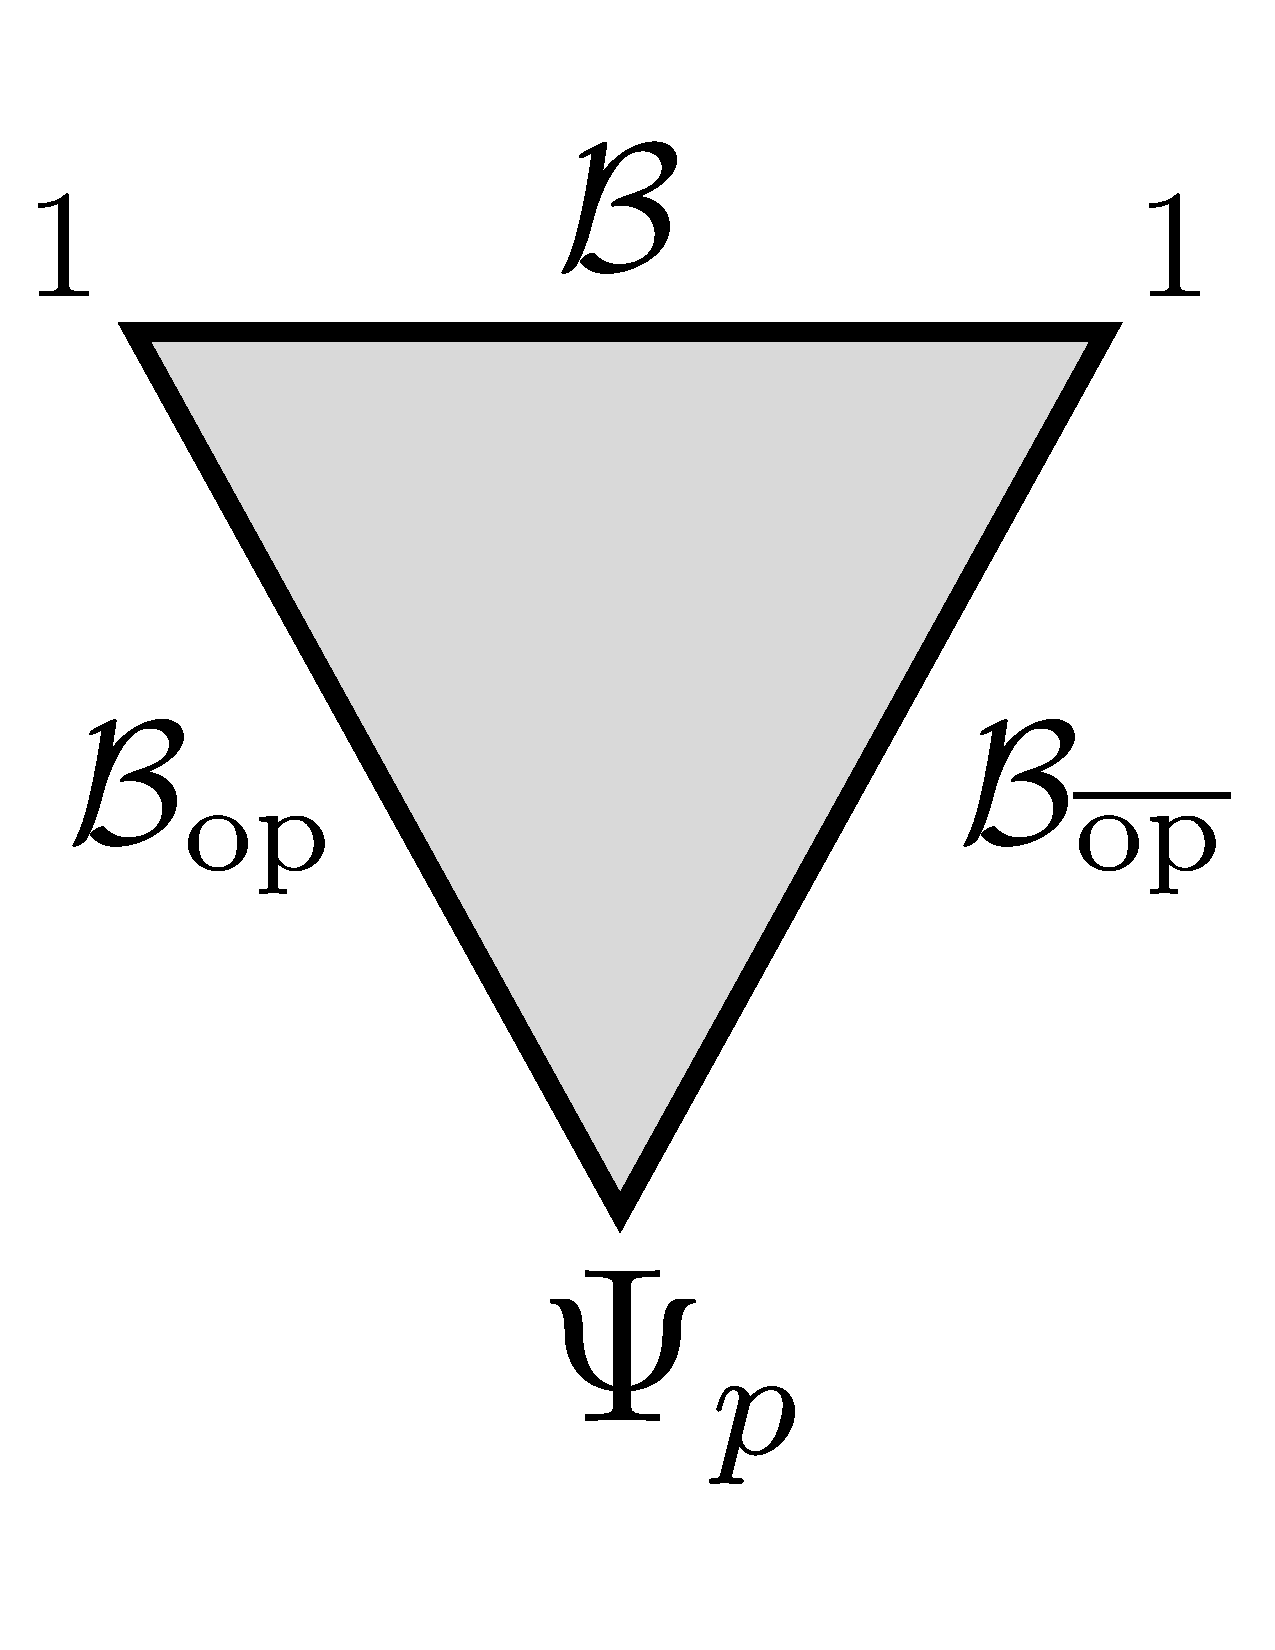
\includegraphics[width=1.2in]{Example10.pdf}
\end{center}
\caption{\small  一个三角形，其底角标以 $\Psi_p\in \Hom(\B_\bop,\B_\op)$，其余各角标以膜 $\B_\op$、$\B_\bop$ 与正则 Nahm 极点的对偶 $\B$ 之间的典范角。这个三角形上的路径积分计算 $(\chi,\Psi_p)$。 \label{example10}}
\end{figure}

我们加在 $\Psi_p$ 上的归一化条件还有另一种解释。我们在第 \ref{nbc} 节已说明，把 $\Psi_p$ 与 $A$-模型中由与正则 Nahm 极点（Nahm pole）相联系的膜 $\B_N$（带适当的角）所生成的态作内积是有意义的，尽管该膜的支撑完全在 $T^*\M(G,C)$ 之外。这个计算在 $B$-模型中其实相当直接。$\B_N$ 的 $B$-模型对偶就是 $\M_H$ 的结构层（structure sheaf）；也就是说，它是支撑为整个 $\M_H$、带平凡 $\CP$（Chan–Paton）丛的秩 1 膜 $\B$。$\B$ 与 $\B_\cc$ 有一个典范角，对应于两膜支撑之交（即 $\M_H\cap L_\op=L_\op$）上的常值函数 1。同样，$\B$ 与 $\bar\B_\cc$ 有一个典范角，由 $\M_H\cap L_{\bop}=L_{\bop}$ 上的函数 1 代表。设 $\chi\in \Hom(\bar\B_\cc,\B_\cc)$ 是由带这些典范角的膜 $\B$ 所生成的态。$B$-模型配对 $(\chi,\Psi_p)$ 由三角形（图 \ref{example10}）上的路径积分计算，该三角形的边标以膜 $\B$、$\B_\cc$ 与 $\bar\B_{\cc}$，其角标以 $\B$ 的典范角与态 $\Psi_p$。$B$-模型局域化到常值映射上；在此情形下，唯一满足必要条件的常值映射是把三角形映到点 $p$ 的常值映射。我们已取所有波函数都等于 1。因此 $(\chi,\Psi_p)=1$。换言之，Hitchin 哈密顿量的本征态 $\Psi_p$ 上那个导致此前关于其希尔伯特空间范数的预言的归一化条件，就是 $(\chi,\Psi_p)=1$。若能在 $A$-模型一侧计算 $(\chi,\Psi_p)$，就会纯粹以 $A$-模型的术语给出 $\Psi_p$ 希尔伯特空间范数的一个预言。配对 $(\chi,\Psi_p)$ 与几何朗兰兹的范畴化方法中的 Whittaker 系数（Whittaker coefficient）有些类似。

% ch16: 原文 GLDraft_D.tex 行 3803–4099；附录 C（3803–3854）与附录 D（3855–4099）
% 只译散文（标题、正文、图题、脚注）；公式、\label、\ref、\eqref、\cite、图文件名保持不变。

\section{典范 oper 截面之间关系的一些例子}\label{somex}
\subsection{$\SL(2,\C)$ 的情形}

基本表示有一组由典范截面（canonical section）构成的基：$s_2 \equiv s$、$Ds$，其中 $D^2 s = t s$。\zy{译者按（依据 \cite{BD} 的一般理论）：这里的“典范截面”指基本截面 $s$ 的对称幂 $s^{\otimes n}$；其各阶导数由 $s$ 与 $Ds$ 的对称化张量积 $s^{\otimes(n-k)}Ds^{\otimes k}$ 给出。在 $\SL(2,\C)$ 情形，一个 oper 由 $C$ 上的一个射影结构连同 $K^{1/2}$（即自旋结构）的一个选择组成；选定自旋结构后，$D^2s=ts$ 就是相应的二阶微分方程。}
$\SL(2,\C)$ 的不可约表示都可以写成基本表示的对称积。
对称幂 $s^{\otimes n}$ 给出 $(n+1)$ 维表示中的典范截面 $s_{n+1}$。$s_{n+1}$ 满足什么微分方程？
在把每个 $D^2 s$ 都换成 $t s$ 之后，对象 $D^r s_{n+1}$（$r\leq n$）可以写成 $s^{\otimes (n-k)} Ds ^{\otimes k}$（$k\leq r$）的对称化形式的线性组合。
到 $n+1$ 阶时不再出现新的对象，于是得到一个微分方程。例如，
\begin{equation}
D^3 s_3= D^2(s \otimes Ds + Ds \otimes s) =2 D(Ds \otimes Ds + 2 t s \otimes s) = 6 t Ds_3 + 4 Dt s_3.
\end{equation}


在把表示相乘时，反对称化可以利用 $s \wedge Ds=1$ 化简。例如，有
\begin{equation}
s_2 \otimes Ds_2 = \frac12 D s_3 + \frac12 s_1
\end{equation}
其中 $s_1=1$，并且我们省略了 $2 \otimes 2 = 3\oplus 1$ 的嵌入映射。我们甚至可以写成一个算子乘积展开（OPE）：
\begin{equation}
s_2(z) \otimes s_2(w) = s_3(w) + \frac12(z-w)Ds_3(w) + \cdots - \frac12 (z-w) s_1(w)+ \cdots
\end{equation}
 
\subsection{$\SL(3,\C)$ 的情形}
基本表示有一组由截面构成的基：$s_3 \equiv s$、$Ds$、$D^2s$，其中 $D^3 s = t_2 Ds +t_3 s$。
外积 $s_{\bar 3} = s_3 \wedge Ds_3$ 是反基本表示中的一个典范截面。确实有
\begin{equation}
D^3s_{\bar 3} = D^2(s_3 \wedge D^2s_3) = D(D s_3 \wedge D^2s_3+t_2 s_3 \wedge D s_3) = t_2 Ds_{\bar 3} + (D t_2-t_3) s_{\bar 3}
\end{equation}

平方 $s_{6,5} = s_3 \otimes s_3$ 是对称平方表示的一个典范截面。
前五个导数 $D^n s_{6,5}$ 是独立的。第六个导数可以用较低阶导数表示，但系数是 $t_2$、$t_3$ 及其导数的有理函数。
更好的做法是定义第二个基元素
\begin{equation}
s_{6,1} \equiv s_3 \otimes D^2 s_3 + D^2 s_3 \otimes s_3 - D s_3 \otimes Ds_3- t_2 s_3 \otimes s_3
\end{equation} 
于是得到如下形式的关系
\begin{align}
&D^5 s_{6,5}- 5 t_2 D^3 s_{6,5}+ (7 t_3 + 4 D t_2)D^2 s_{6,5} + \cdots = (4 t_3 - 2 D t_2) s_{6,1} \cr
&D s_{6,1} = (2 t_3- D t_2) s_{6,5} 
\end{align} 
\zy{译者按（无外部依据）：由下文可见，$s_{6,5}$、$s_{6,1}$、$s_{8,5}$、$s_{8,3}$ 的第二个下标是相应截面所满足的微分方程的阶（亦即其独立导数的个数）：例如 $s_{6,5}$ 满足 5 阶方程，$s_{8,3}$ 满足 3 阶方程。}
我们可以把这些关系以及更多关系概括进一个 OPE
\begin{equation}
s_3(z) \otimes s_3(w) \sim s_{6,5} + \cdots + \frac12 (z-w) s_{\bar 3} +\cdots + \frac14 (z-w)^2 s_{6,1} + \cdots
\end{equation}

注意 $s_3$ 与 $s_{\bar 3}$ 彼此正交，因此 $s_{8,5} = s_3 \otimes s_{\bar 3}$ 是一个典范的伴随截面，而
 $s_{8,3} = s_3 \otimes D s_{\bar 3}-D s_3 \otimes s_{\bar 3}$ 是第二个。它们满足预期形式的微分方程
 $D^5 s_{8,5} = \cdots$ 与 $D^3 s_{8,3}= \cdots$，并且两个方程的右端都同时出现这两个截面的导数。
 
 
 \section{波函数奇异行为的局部模型}\label{localmodel}
 
 \subsection{摇摆除子}\label{wobbly}
 
如第 \ref{wkb} 节所讨论，Hecke 算符或 Hitchin 哈密顿量的本征函数 $\Psi$ 自然地由一张秩 1 拉格朗日膜 $\B_F$ 表示，该膜支撑在 Hitchin 纤维化的一个纤维 $F$ 上。$F$ 必须满足量子修正后的 WKB 条件。
 
为了把 $\Psi$ 表示成 $\M(G,C)$ 上的显式半密度，可以取它与 delta 函数态 $\delta(x,x_0)$ 的内积，得到 $\Psi(x_0)=\la \delta(x,x_0),\Psi\ra$。delta 函数态 $\delta(x,x_0)$ 由一张拉格朗日膜 $\B_{x_0}$ 表示，该膜支撑在余切
丛 $T^*\M(G,C)\to \M(G,C)$ 于 $x_0\in \M(G,C)$ 处的纤维 $L_{x_0}$ 上。尽管内积 $\la \delta(x,x_0),\Psi\ra$ 的计算是一个困难问题，多半不会有相当显式的答案，但它是良定义的；只要 $\M_H(G,C)$ 的 $A$-模型中的膜 $\B_{x_0}$ 良定义并随 $x_0$ 实解析地变化，所得结果就会随 $x_0$ 实解析地变化。而这又只要
$L_{x_0}$
在 $\M_H(G,C)$ 中是闭的便成立。
 
然而已知，这一结论沿一个除子 $\sD\subset \M(G,C)$ 失效，该除子有时被称为摇摆除子（wobbly divisor；参见例如 \cite{DP,PP,PPN,HZ}）。稳定丛 $E\to C$ 称为非常稳定的（very stable），如果任何幂零的希格斯场 $\varphi:E\to E\otimes K$ 实际上都是 0。反之，若存在某个幂零且非零的 $\varphi:E\to E\otimes K$，则称 $E$ 是摇摆的。除子 $\sD$ 参数化摇摆丛。\zy{译者按：原文所引 \cite{PP} 的原题为“The Wobbly Divisors of the Moduli Space of Rank-2 Vector Bundles”，\cite{PPN} 则讨论“Very Stable Bundles and Properness of the Hitchin Map”（Hitchin 映射的紧合性）。“摇摆”与“非常稳定”是互补的：非常稳定丛不允许非零幂零希格斯场，摇摆丛则允许。}
 
膜的支撑集必须是闭的，因此当 $L_{x_0}$ 不是闭集时，它就不能作为膜的支撑集。于是波函数 $\Psi(x_0)$ 可能沿 $\sD$ 变奇异。
 
在本附录中，我们将对 $G=\SU(2)$ 的情形分析沿 $\sD$ 的行为；稍作改动，讨论也适用于 $G=\SO(3)$。对于带抛物结构的丛，亏格 0 情形已有关于 Hecke 算符与 Hitchin 哈密顿量本征函数行为的显式计算 \cite{EFK3}。尽管我们在本文中没有显式纳入抛物结构，在本附录中也不会这样做，但我们的全部考虑都自然推广到带抛物结构的丛。（在规范场论中，抛物结构是通过纳入某一类与余维 2 奇点相伴的面算符来描述的 \cite{GuW2}。）因此，我们将把我们的结果与 \cite{EFK3} 中已得到的结果作比较。
 
以下 $C$ 是亏格为 $g$ 的黎曼曲面，其典范丛为 $K$、切丛为 $T$；$E\to C$ 是秩 2 的全纯向量丛，$\det\,E$ 平凡。
若 $E$ 不是非常稳定的，则存在非零希格斯场 $\varphi:E\to E\otimes K$ 使 $\varphi^2=0$。此时 $E$ 有直线子丛 $\L=\mathrm{ker}\,\varphi$，因此 $E$ 是一个扩张
\be\label{extform} 0\to \L \to  E\to \L^{-1}\to 0.\ee
我们关心非平凡扩张，但希望与直和 $E_0=\L\oplus \L^{-1}$ 作比较。我们主要关心的情形将是：$E_0$ 不稳定，而 $E$ 稳定。若满足下述条件，这一点对一般情形成立：\footnote{次数为 0 的秩 2 丛 $E\to C$ 稳定，当且仅当它的任何秩 1 子丛 $\M\subset E$ 的次数都为负。
若 $E$ 有一个次数为 0 的直线子丛，但没有正次数的直线子丛，则称它是半稳定的。
按定义，正合列 (\ref{extform}) 中的 $E$ 有子丛 $\L$；若 $\L$ 的次数为负，这不会使 $E$ 不稳定（而且出现在这种正合列中的 $E$ 一般都是稳定的）。然而，当 $\L$ 的次数为负时，$\L^{-1}$ 的次数为正，直和 $E_0=\L\oplus \L^{-1}$ 不稳定。}
$$c_1(\L)<0. $$
对一般的 $\L$，$E_0$ 作为 $\SL(2,\C)$ 丛的自同构群是由对角矩阵构成的群，我们把它记作 $P$。

此情形下的幂零希格斯场为 $\varphi_0\in H^0(C,\Hom(\L^{-1},\L\otimes K))=H^0(C, \L^2\otimes K)$。可以预期，在摇摆除子 $\sD$ 的一般点上，幂零希格斯场的空间是 1 维的，因此我们预计会需要\footnote{$H^q(C,\M)$ 的维数记作 $h^q(C,\M)$，或简记作 $h^q(\M)$。} $h^0(\L^2\otimes K)= 1$。
为简单起见，我们将研究 $\sD$ 的一个分支，它具有如下性质：在 $\sD$ 内，$\L$ 可以一般地形变（只固定 $c_1(\L)$）。
（$\sD$ 中存在一些分支，上述性质对它们不成立；这些分支可以用类似方式研究，结果也类似。）
在这一假设下，要求一般情形下 $h^0(\L^2\otimes K)$ 为 1，
就推出一般情形下 $h^1(\L^2\otimes K)$ 为 0，而 $\L$ 的次数由 Riemann–Roch 公式确定：
\be\label{degl} 1=h^0(\L^2\otimes K)-h^1(\L^2\otimes K) = 1-g+ c_1(\L^2\otimes K)=g-1 +2c_1(\L)\ee
于是
\be\label{egf}c_1(\L)=1-\frac{g}{2},\ee
因此，如上所述的构造只对偶数 $g$ 可能。不过，对奇数 $g$，我们可以做非常类似的事情：$c_1(\L)$ 的半整数值
意味着我们应当取规范群为 $\SO(3)$ 而非 $\SU(2)$，并把 $E$ 处处替换为 $\ad(E)$。
由于记号上更简单，我们将继续使用
$\SU(2)$ 规范场论的语言，但下面的评注也适用于另一情形。
对 $g>2$，$c_1(\L)<0$，因此如式 (\ref{extform}) 那样的扩张 $E$ 可以是稳定的，而直和 $E_0$ 不稳定。对 $g=2$，$E$ 可以稳定，而 $E_0$ 半稳定。\zy{译者按（无外部依据）：$g$ 为奇数时 $c_1(\L)=1-g/2$ 是半整数，不可能是一个 $\SU(2)$ 丛的直线子丛的次数；把规范群换成 $\SO(3)=\SU(2)/\Z_2$ 后，$\ad(E)$ 是相应的伴随三维向量丛（伴随表示即其标准三维表示），$\L$ 则只以“分数次”线丛的意义出现。}

条件 $h^0(\L^2\otimes K)=1$ 与 $h^1(\L^{-2})=1$ 互为 Serre 对偶。由于 $H^1(C,\L^{-2})$ 参数化 $E_0$ 的{\it 不}
保持三角结构 (\ref{extform}) 的形变（而不保持这一结构的 $E$ 的形变计数相同），条件
$h^1(\L^{-2})=1$ 确实是我们所需要的，它使得我们所讨论的结构在 $\M(G,C)$ 中以余维 1 出现，从而可以代表沿 $\sD$ 的一般行为。
现在也可以数出 $E_0$ 的{\it 确实}具有式 (\ref{extform}) 三角结构的形变。
这个形变空间的维数是
$h^1(\L^2)=g-1-2c_1(\L) =2g-3$。作为检验，通过形变 $E_0$ 得到的稳定丛族的维数是
$h^1(\ad(E_0)) - h^0(\ad(E_0))-\mathrm{dim}\,P = g + (2g-3)+1 -1 =3g-3$，正是预期值。（我们计入了 $E_0$ 的 $g$ 个对角形变。
在计算 $E_0$ 的形变参数空间时，
我们减去 ${\mathrm{dim}}\,P=1$，以计入一般形变会破坏 $E_0$ 的 $P$-不变性这一事实。）
为下文方便，定义
\be\label{weddo} N = h^1(\L^2)= 2g-3,\ee
即沿除子 $\sD$ 的不稳定丛 $E_0$ 的上三角部分的形变数目。因此，如上所述的构造只给出 $N$ 的正奇数值；
不过，正偶数值可以通过带抛物结构的类似构造，或通过放弃“$\L$ 可以在保持在 $\sD$ 内的同时任意形变”这一假设来得到。



现在我们来考察此情形下希格斯丛模空间的局部行为。
取基使 $E_0=\begin{pmatrix}\L\cr \L^{-1}\end{pmatrix}, $ 则不稳定丛 $E_0$ 可以由一个 $\bar\partial$ 算子显式描述：
\be\label{barpar}\bar D=\bar\partial +\begin{pmatrix} a_0 & 0 \cr 0 & -a_0\end{pmatrix}. \ee
下文中，改变 $\L$ 的“对角”形变并不重要，因为我们已假设任何一般的 $\L$（具有适当的次数）
都能导致我们所考虑的情形。换言之，我们的假设使得 $\L$ 的形变只是让我们沿着 $\sD$ 移动。
出于同样理由，我们对对角希格斯场也不感兴趣。
相反，我们必须考察“上对角”与“下对角”形变，它们使我们离开 $\sD$。
按我们的假设，上对角丛形变的空间
维数为 $N$，下对角丛形变的空间维数为 1。我们取 $H^1(C,\L^2)$ 的一组基 $b_1,\cdots, b_n$，并把
该群的一般元素写成 $\sum t_i b_i$，其中 $t_i$ 为复参数。类似地，取非零的 $c\in H^1(C,\L^{-2})$，并把一般
元素写成 $uc$，其中 $u$ 为复参数。
于是 $\bar D$ 的一般非对角扰动给出
\be\label{arpar}\bar D'=\bar D +\begin{pmatrix} 0 & \sum_{i=1}^n t_i b_i \cr uc & 0  \end{pmatrix}. \ee
类似地，对希格斯场，引入非零元素 $e$（取自 $H^0(C, K\otimes \L^2)$）以及 $H^0(C,K\otimes \L^{-2})$ 的一组基 $f_1,f_2,\cdots,f_N$，
再引入额外的复参数 $s$ 与 $r_1,r_2,\cdots, r_N$，则希格斯场的非对角部分为
\be\label{offed}\varphi_\perp =\begin{pmatrix} 0 & se \cr \sum_{i=1}^N r_i f_i&0 \end{pmatrix}. \ee
对这些数据，需要施加希格斯丛方程 $[\bar D',\varphi_\perp]=0$。由于由 $\varphi_\perp$ 的定义
已有 $[\bar D,\varphi_\perp]=0$，该条件约化为 $\mu=0$，其中
\be\label{kinny} \mu=\sum_{i=1}^N r_i t_i -su. \ee 
（这里通过适当归一化波函数，把某些常数取成了 1。）
为了得到希格斯丛模空间的局部描述，更确切地说，得到它横截于那些无关紧要的对角形变的一个切片，我们还
必须除以 $P\cong \C^*$，即不稳定丛 $E_0$ 的自同构群。$P$ 以如下权作用在这些变量上：上对角
参数 $t_i$ 与 $s$ 的权为 1，下对角参数 $u$ 与 $r_i$ 的权为 $-1$。除以 $P$ 并施加条件
(\ref{kinny}) 的联合操作有一个简单的解释。引入辛形式
\be\label{inny}\Omega = \sum_{i=1}^N \d r_i\, \d t_i +\d s \,\d u, \ee 
便看出 $\mu$ 是 $P$ 作用在这些参数上的矩映射。令 $\mu=0$ 并除以 $P$
的联合操作是一个复辛商，其结果将是一个复辛流形，正如希格斯丛模空间所应有的那样。

然而，我们必须小心“商”的含义。若一个希格斯丛中所有权为 1 的参数 $t_i$ 与 $s$ 都为零，
则它不稳定。\footnote{设 $E$ 是行列式平凡、秩为 2 的丛。若 $E$ 有一个正次数的 $\varphi$-不变子丛，则希格斯丛 $(E,\varphi)$ 不稳定。若 $E$ 有一个次数为零的 $\varphi$-不变子丛，但没有正次数的此类子丛，则称 $(E,\varphi)$ 半稳定。
若 $E$ 有一个正次数子丛，但 $E$ 的任何 $\varphi$-不变子丛次数都为负，则丛 $E$ 不稳定，而希格斯丛 $(E,\varphi)$ 稳定。在目前的例子中，若 $t_i=s=0$，则 $E$ 有正次数的 $\varphi$-不变子丛 $\L^{-1}$。}因此我们希望带上 Mumford 稳定性条件来取商，使得 $t_i$ 与 $s$ 不允许全部为零。于是，在 $P$ 的作用之下，$N+1$ 个变量
$t_i$ 与 $s$ 定义 $\bCP^N$ 中的一个点，而由此构造得到的希格斯丛模空间的局部模型便是
\be\label{hb} M_H= T^*\bCP^N. \ee
更确切地说，这是横截切片，抓住了希格斯丛模空间在 $\sD$ 附近的相关方面。

那么，半稳定丛的模空间 $M$ 的相应局部模型又如何呢？为此我们忘掉希格斯参数 $s$ 与 $r_i$，
只保留丛参数 $t_i$ 与 $u$。若令所有 $t_i$ 为零，便得到不稳定丛。因此 $t_i$ 取为不全为零，而在 $P$ 的作用下，它们定义 $\bCP^{N-1}$ 中的一个元素。
把权为 $-1$ 的变量 $u$ 考虑进来，便看出
$M$ 的局部模型是线丛 $\O(-1)\to \bCP^{N-1}$ 的全空间。这与在一点处爆破 $\C^N$ 相同。
不是非常稳定的丛构成的除子 $\sD$ 在这个模型中由方程 $u=0$ 定义；换言之，它就是例外除子
$\bCP^{N-1}\subset M$。方便的做法是定义 $x_i= u t_i$。于是 $M$ 由 $x_i$ 参数化，而点 $\vec x=0$ 被爆破。
至于与 $x_i$ 典范共轭的变量，可以取 $p_i=r_i/u$，因为
\be\label{wobo}\Omega =\sum_{i=1}^N \d p_i \d x_i. \ee
当然，这些坐标在例外除子附近并不好用。

$N=1$ 的情形在许多方面都是例外。
对 $N=1$，丛 $E_0$ 是半稳定的而非不稳定的，因为 $\L$ 的次数为 0。此外，对 $N=1$，刚才描述的构造中实际上没有爆破。只有当 $N>1$ 时，除子
$\sD\cong \bCP^{N-1}\subset M$ 才是摇摆的。对 $N=1$，它是半稳定的；也就是说，它参数化一族半稳定丛。

现在我们可以解释本附录开头所作的断言：沿摇摆
除子，丛模空间的余切丛的纤维在希格斯丛模空间中不是闭的。在这一分析中，我们
把丛模空间 $\M(G,C)$ 与 $\M_H(G,C)$ 替换为它们的局部模型 $M$ 与 $M_H$。

首先考虑 $M$ 中不在 $\sD$ 内的一个点。$\sD$ 在 $M$ 中的补集由非零的 $N$ 元组 $\vec x=(x_1,x_2,\cdots, x_N)$ 构成。
例如，取由 $x_1\not=0$、$x_2=\cdots= x_N=0$ 定义的点 $p$。由于 $x_1=ut_1$，$x_1\not=0$
意味着 $u$ 与 $t_1$ 都非零。我们可以用 $P$ 的作用固定
$t_1=1$。希格斯场受以下条件约束：
\be\label{higgscon} r_1-su=0, \ee
而对 $r_2,\cdots, r_N$ 没有约束。在利用式 (\ref{higgscon}) 解出 $r_1$（用 $s$ 表示）之后，我们看到 $p$ 处的希格斯场空间
由 $s,r_2, \cdots, r_N$ 参数化。这是预期的 $\C^N$；它是 $M$ 的余切丛在 $p$ 处的纤维，并且在 $\M_H$ 中是闭的。我们将把它记作 $L_p$。现在换而考察
余切丛在点 $p'\in \sD$ 处的纤维。为此，只需取 $u=0$，仍令 $t_1=1$ 以及 $t_i=0,$ $i>1$。式 (\ref{higgscon})
仍然成立，并告诉我们令 $r_1=0$，而对 $u$ 没有约束。因此在这种情况下，余切纤维 $L_{p'}$ 仍由
$s$ 与 $r_2,\cdots, r_N$ 参数化。但 $L_{p'}$ 在 $M_H$ 中不是闭的。为看出这一点，考虑 $\C\subset L_{p'} $ 的一个拷贝，它由 $(t_1,s)=(1,\lambda),\,\lambda\in\C$
与 $r_2=\cdots = r_N=0$ 定义。在 $P$ 的作用下，条件 $(t_1,s)=(1,\lambda)$ 等价于 $(t_1,s)=(1/\lambda,1)$。
显然，极限 $\lambda\to\infty$ 存在。
因此这个 $\C$ 的拷贝在 $M_H$ 中不是闭的；它的闭包包含一个 $(t_1,s)=(0,1)$ 的点，从而把 $\C$ 紧化为 $\bCP^1$。更一般地，$L_{p'}$ 在 $M_H$ 中的闭包
由 $(t_1,s,r_2,\cdots, r_N)$ 模去 $P$ 的作用来参数化，并带有一个约束：$t_1$ 与 $s$ 不允许同时为零。它是 $\bCP^1$ 上的一个 $\C^{n-1}$ 丛。满足
$t_1=0$、$s\not=0$ 的点对应于这样的希格斯丛 $(E_0,\varphi)$：底层丛 $E_0$ 不稳定，但配对 $(E_0,\varphi)$
稳定。这些点包含在 $M_H$ 中，但不包含在 $T^*M$ 中。若令 $t_1=s=0$，便得到不稳定的希格斯丛。

现在让我们回到一般点 $p\in M$（它不包含在 $\sD$ 内），并问当 $p$ 趋近 $\sD$ 时 $L_p$ 会怎样。我们考虑与
前面相同的点 $p$，但既然现在知道允许 $t_1=0$ 很重要，我们就不令 $t_1=1$，而把约束 (\ref{higgscon}) 写成：
\be\label{iggscon} t_1 r_1-su=0. \ee
我们还有点 $p$ 的定义：
\be\label{defp} ut_1= x_1.\ee
$L_p $ 由满足这些方程的 $t_1,u,s$ 与 $r_1,r_2\cdots, r_N$ 参数化，再模去 $P$ 的作用。
为了取 $p\to p'$ 时 $L_p$ 的极限，只需在式 (\ref{defp}) 中令 $x_1=0$。所得簇有两个分支。在一个分支上，
$u=r_1=0$，而 $t_1,s$ 一般非零。这个分支（我们称之为 $L_{p',1}$）就是前面描述过的 $L_{p'}$ 在 $M_H$ 中的闭包；它是 $\bCP^1$ 上的一个 $\C^{N-1}$ 丛。在第二个分支上，$t_1=0$，于是 $s$ 必须非零（为使 $(E,\varphi)$ 稳定），从而式
(\ref{iggscon}) 蕴含 $u=0$。第二个分支是 $\C^N$ 的一个拷贝，由 $r_1,\cdots, r_N$ 参数化。由于 $t_1=u=0$，这第二个分支 $L_{p',2}$
完全包含在 $M_H$ 中 $T^*M$ 的补集内。

对一般的 $p$，存在一张秩 1 的 $A$-膜 $\B_p$ 支撑在 $L_p$ 上；由于 $L_p \cong \C^N$ 单连通，它是唯一的。当 $p\to p'$ 时，
$L_p$ 分裂成两个分支，其中任何一个都可以支撑一张 $A$-膜。由于 $\B_p$ 只在远离摇摆除子处光滑变化，
Hitchin 哈密顿量的本征函数有可能沿该除子变奇异。
我们将在第 \ref{singular} 节研究这个问题。

对 $N=1$，没有摇摆除子，上述构造中也没有爆破。（亏格 2 的模空间确实有摇摆除子，但不具有
我们所假设的那些性质。）$N$ 元组 $(t_1,\cdots, t_N)$ 退化为单个变量
$t$，而模空间 $M$ 在这个局部模型中是由 $x=ut$ 参数化的 $\C$ 的一个拷贝。$x=0$ 处的行为是例外的，但原因
不同。在 $x=0$ 处，丛 $E$ 退化为直和 $E_0=\L\oplus \L^{-1}$，而它在 $N=1$ 时是半稳定的。沿除子 $\sD$ 存在未破缺的 $\U(1)$ 规范对称性，在理解沿
该除子的行为时必须把它考虑进去。

\subsection{波函数的奇异行为}\label{singular}





一般的 Hitchin 哈密顿量是 $\int_C \alpha \Tr \varphi^2$，
其中 $\alpha\in H^1(C,T)$。由于式 (\ref{offed}) 中希格斯场 $\varphi$ 的形式，任何这样的哈密顿量对 $s$ 是 1 次齐次的，同样对 $r_i$ 也是 1 次齐次的。由于线性无关的 Hitchin 哈密顿量的数目
与希格斯丛参数的数目相同，我们可以一般地选取一组 Hitchin 哈密顿量，使得
\be\label{genbas} H_i = s r_i,~~~i=1,\cdots,N.\ee（由于还存在我们忽略掉的对角扰动，这
并不是 Hitchin 哈密顿量的全集。它是在这一近似下依赖于非对角扰动的那一组 Hitchin 哈密顿量。）

用远离原点处好用的典范变量 $p_i, x_i$ 表示，它便是 $H_i=p_i\sum_{k=1}^N x_k p_k$。量子化之后，
它成为
\be\label{qut} H_i=\frac{1}{2}\sum_{k=1}^n \left(\frac{\partial}{\partial x_i} x_k \frac{\partial}{\partial x_k}+\frac{\partial}{\partial x_k} x_k\frac{\partial}{\partial x_i}\right). \ee
选取这样的算符次序，是为了使这些算符形式对称（已知 Hitchin 哈密顿量具有这一性质）。
$H_i$ 作用在如下半密度上：
\be\label{murky} F(x_1,x_2,\cdots, x_N)(\d x_1\d x_2\cdots \d x_N)^{1/2}. \ee
当然，式 (\ref{qut}) 中写下的并不是 Hitchin 哈密顿量的精确公式。
它只是对小 $\vec x$ 有效的渐近公式。考虑一个标度变换，使 $x, p$ 的权分别为 $1,-1$。
式 (\ref{qut}) 中的算符 $H_i$ 以权 $-1$ 标度。这里的主张是：Hitchin 哈密顿量由这些表达式给出，模去
非负权的项。

要用这个模型预测 Hitchin 哈密顿量本征函数在例外除子 $\sD$ 附近的行为，我们需要使用
在 $\sD$ 附近好用的坐标。一个方便的选择是使用 $x_1$ 以及 $y_k=x_k/x_1$（$k=2,3,\cdots,N$）。这些坐标
在 $\sD$ 中一个大的开集附近是好用的。

除了把变量从 $x_1,x_2,x_3,\cdots,x_N$ 换为 $x_1,y_2,y_3,\cdots, y_N$，我们还希望以一种在这些坐标下自然的方式表示半密度。
一个适当的形式是
\be\label{urky} G(x_1,y_2,\cdots, y_N) (\d x_1 \d y_2 \d y_3\cdots \d y_N)^{1/2}. \ee
于是 $F$ 与 $G$ 之间的关系应为
\be\label{rky} F(x_1,x_2,\cdots,x_N)=x_1^{-(N-1)/2} G(x_1,y_2,\cdots, y_N), \ee
从而 $F(x_1,\cdots, x_N)(\d x_1\cdots \d x_N)^{1/2}=G(x_1,y_2,\cdots, y_N) (\d x_1 \d y_2\cdots \d y_N)^{1/2}$。
作用在 $G$ 上的 Hitchin 哈密顿量在新坐标下成为
\begin{align} H_1& = \frac{\partial}{\partial x_1}x_1\frac{\partial}{\partial x_1} -\frac{1}{2}\sum_{k=2}^N\left( y_k \frac{\partial}{\partial y_k}+\frac{\partial}{\partial y_k} y_k\right)
\frac{\partial}{\partial x_1} \cr
H_k& =\frac{\partial^2}{\partial x_1 \partial y_k},~~~~~~~~ k>1. \end{align}
寻找在 $x_1\to 0$ 时表现为 $x_1^\alpha$ 的联合本征函数，可以看出：对偶数 $N$，可能值为 $\alpha=0$ 与 $\alpha=(N-1)/2$，
这与亏格 0 情形抛物丛的计算 \cite{EFK3} 一致。对于奇异解 $x_1^{(N-1)/2}g(x_1,\vec y)$（其中 $g(x_1,\vec y)$
在 $x_1=0$ 处全纯），$g(x_1,\vec y)$ 在 $x_1=0$ 处实际上与 $\vec y$ 无关。对奇数 $N$，相应的陈述是：除全纯
解之外，
还有形如
  $f(x_1,\vec y)+g(x_1,\vec y)x_1^{(N-1)/2}\log x_1$ 的解，其中 $f(x_1,\vec y)$ 与 $g(x_1,\vec y)$ 在 $x_1=0$ 处全纯，并且同样 $g(x_1,\vec y)$
  在 $x_1=0$ 处与 $\vec y$ 无关。
  
  
 
这些公式只抓住了除子 $D$ 附近最奇异的一些项，行为相当非一般。
特别地，本征值方程 $H_s\Psi=\lambda_s\Psi$（$s=1,\cdots, N$）没有预期的 $2^N$ 个线性无关联合解。
若给 Hitchin 哈密顿量加上一般的高阶项而保持其交换性，预期的行为就会恢复。
例如（把 $\partial/\partial x_1$ 简写为 $\partial_1$，把 $\partial/\partial y_k$ 简写为 $\partial'_k$），一个使 Hitchin
哈密顿量的交换性保持到 $\alpha$ 一阶的简单扰动，就是把上面的公式替换为
\begin{align}\label{perturbed} \t H_1& = \partial_1 x_1\partial_1 -\frac{1}{2}\sum_{k=2}^N(y_k \partial'_k+\partial'_k y_k)\partial_1
+2 \sum_{l,m=2}^N \alpha_{klm}\partial'_l y^k \partial'_m \cr
\t H_k&= \partial_1\partial'_k +\sum_{l,m=2}^N \alpha_{klm}\partial'_l\partial'_m,~~~~~k>1, \end{align}  
其中 $\alpha_{klm}=\alpha_{kml}$ 是一般的复系数。奇异行为与前面类似。

\begin{yizhu}[译者按：原文笔误与记号]
本块原文有几处笔误；公式与记号中的笔误在译文中照原样保留，拼写错误则按正确词义译出，不另作径改。
(1) 本块第一式（$D^3s_3=\cdots$）的中间式与末式系数有误。按 $D^2s=ts$ 直接计算，
$D^2(s\otimes Ds+Ds\otimes s)=2D(Ds\otimes Ds+t\,s\otimes s)$，
故 $D^3s_3=4t\,Ds_3+2Dt\,s_3$；原文分别写作 $2t$、$6t$、$4Dt$。
(2) 拼写：“with we will call $P$”应为“which we will call”；“By constrast”应为“By contrast”；“divsor”应为“divisor”；“suppport”应为“support”。
(3) 式 (\ref{arpar}) 前的 $b_1,\cdots, b_n$ 与式中的 $\sum_{i=1}^n$，式 (\ref{qut}) 中的 $\sum_{k=1}^n$，以及 $L_{p'}$ 闭包的纤维 $\C^{n-1}$，按上下文均应为大写 $N$。
(4) “near the divisor $D$”中的 $D$ 应为 $\sD$（摇摆除子）。
(5) 式 (\ref{perturbed}) 第一行中 $\alpha_{klm}\partial'_l y^k\partial'_m$ 的指标 $k$ 未求和，使 $\t H_1$ 依赖于一个未指定的 $k$，疑有笔误；译文照录。
(6) 本块“$h^1(\ad(E_0))-h^0(\ad(E_0))-\dim P=g+(2g-3)+1-1=3g-3$”一式的算术与记号疑不一致：按 $h^0=1$、$\dim P=1$，左边应为 $3g-4$；若只减去 $\dim P$，则为 $3g-3$。译文照录，存疑待核。
\end{yizhu}


\clearpage
\phantomsection
\addcontentsline{toc}{section}{参考文献}
% ch17: 原文 GLDraft_D.tex 行 4100–4488；参考文献
% 只译散文（标题、正文、图题、脚注）；公式、\label、\ref、\eqref、\cite、图文件名保持不变。

\begin{thebibliography}{99}
\bibitem{BD}
A. Beilinson and V. Drinfeld, ``Quantization of Hitchin's
Integrable System and Hecke Eigensheaves,''
available at \url{http://www.math.uchicago.edu/~drinfeld/langlands/QuantizationHitchin.pdf}.

\bibitem{F}
E. Frenkel, ``Lectures on the Langlands Program and Conformal Field Theory,'' in P. Cartier, ed., {\it Frontiers in Number Theory,
Physics, and Geometry, II} (Springer, Berlin, 2007) 387-533, hep-th/0512172.

\bibitem{KW}A. Kapustin and E. Witten, 
``Electric-Magnetic Duality and the Geometric Langlands Program,''   Commun. Num. Theor. Phys.
{\bf 1} (2007) 1-236,
arXiv:hep-th/0604151.

\bibitem{BN} D. Ben-Zvi and D. Nadler, ``Betti Geometric Langlands,'' arXiv:1606.08523.

\bibitem{BaDo}
J. C. Baez and J. Dolan, ``Higher Dimensional Algebra
and Topological Quantum Field Theory,'' J. Math. Phys. {\bf 36} (1995) 6073-6105.

\bibitem{L1}
J. Lurie, ``On The Classification of Topological Field Theories,''
in {\it Current Developments in Mathematics} (Int. Press, Somerville, 2009), pp. 129-280, arXiv:0905.0465.

\bibitem{Fr} D. Freed, ``The Cobordism Hypothesis,''  arXiv:1210.5100.

\bibitem{EFK}
P. Etingof, E. Frenkel, and D. Kazhdan, ``An Analytic Version Of The Langlands Correspondence For Complex Curves,''  in S. Novikov et. al., eds.,
{\it Integrability, Quantization, and Geometry II. Quantum Theories and Algebraic Geometry}, Proc. Symp. Pure Math. {\bf 103.2} (American
Mathematical Society, 2021) pp. 137-202,
arXiv:1908.09677.

\bibitem{EFK2}
P. Etingof, E. Frenkel, and D. Kazhdan, ``Hecke Operators and Analytic Langlands Correspondence For Curves Over Local Fields,''
arXiv:2103.01509.

\bibitem{EFK3}
P. Etingof, E. Frenkel, and D. Kazhdan, ``Analytic Langlands Correspondence for $\mathrm{PGL}_2$ on ${\Bbb P}^1$ With Parabolic
Structure Over Local Fields,'' arXiv:2106.05243.

\bibitem{L}
R. Langlands, ``On Analytic Form of Geometric Theory of Automorphic Forms,'' available at
\url{http://publications.ias.edu/sites/default/files/iztvestiya-english_3.pdf}.


\bibitem{T}
J. Teschner, ``Quantization Conditions Of The Quantum Hitchin System and the Real Geometric Langlands Correspondence,'' in J. E. Dancer 
et. al., eds., {\it Geometry and Physics}, vol. 1 (Oxford University Press, 2018),
arXiv:1707.07873.



%\cite{Nekrasov:2009rc}
\bibitem{Nekrasov:2009rc}
N.~A.~Nekrasov and S.~L.~Shatashvili,
``Quantization of Integrable Systems and Four Dimensional Gauge Theories,''
doi:10.1142/9789814304634\_0015
[arXiv:0908.4052 [hep-th]].
%544 citations counted in INSPIRE as of 02 Jul 2021

%\cite{Teschner:2010je}
\bibitem{Teschner:2010je}
J.~Teschner,
``Quantization of the Hitchin moduli spaces, Liouville theory, and the geometric Langlands correspondence I,''
Adv. Theor. Math. Phys. \textbf{15}, no.2, 471-564 (2011)
doi:10.4310/ATMP.2011.v15.n2.a6
[arXiv:1005.2846 [hep-th]].
%114 citations counted in INSPIRE as of 02 Jul 2021


%\cite{Nekrasov:2010ka}
\bibitem{Nekrasov:2010ka}
N.~Nekrasov and E.~Witten,
``The Omega Deformation, Branes, Integrability, and Liouville Theory,''
JHEP \textbf{09}, 092 (2010)
doi:10.1007/JHEP09(2010)092
[arXiv:1002.0888 [hep-th]].
%215 citations counted in INSPIRE as of 02 Jul 2021



%\cite{Nekrasov:2011bc}
\bibitem{Nekrasov:2011bc}
N.~Nekrasov, A.~Rosly and S.~Shatashvili,
``Darboux coordinates, Yang-Yang functional, and gauge theory,''
Nucl. Phys. B Proc. Suppl. \textbf{216}, 69-93 (2011)
doi:10.1016/j.nuclphysbps.2011.04.150
[arXiv:1103.3919 [hep-th]].
%147 citations counted in INSPIRE as of 02 Jul 2021


%\cite{Bonelli:2011na}
\bibitem{Bonelli:2011na}
G.~Bonelli, K.~Maruyoshi and A.~Tanzini,
``Quantum Hitchin Systems via ${\beta}$ -Deformed Matrix Models,''
Commun. Math. Phys. \textbf{358}, no.3, 1041-1064 (2018)
doi:10.1007/s00220-017-3053-0
[arXiv:1104.4016 [hep-th]].
%62 citations counted in INSPIRE as of 02 Jul 2021


%\cite{Nekrasov:2014yra}
\bibitem{Nekrasov:2014yra}
N.~A.~Nekrasov, A.~A.~Rosly and S.~L.~Shatashvili,
``Darboux coordinates, Yang-Yang functional, and gauge theory,''
Theor. Math. Phys. \textbf{181}, no.1, 1206-1234 (2014)
[erratum: Theor. Math. Phys. \textbf{182}, no.2, 368 (2015)]
doi:10.1007/s11232-014-0209-3
%6 citations counted in INSPIRE as of 02 Jul 2021


%\cite{Balasubramanian:2017gxc}
\bibitem{Balasubramanian:2017gxc}
A.~Balasubramanian and J.~Teschner,
``Supersymmetric field theories and geometric Langlands: The other side of the coin,''
Proc. Symp. Pure Math. \textbf{98}, 79-106 (2018)
[arXiv:1702.06499 [hep-th]].
%6 citations counted in INSPIRE as of 02 Jul 2021


%\cite{Jeong:2018qpc}
\bibitem{Jeong:2018qpc}
S.~Jeong and N.~Nekrasov,
``Opers, surface defects, and Yang-Yang functional,''
[arXiv:1806.08270 [hep-th]].
%31 citations counted in INSPIRE as of 02 Jul 2021



\bibitem{GuW}S. Gukov and E. Witten, ``Branes and Quantization,'' ATMP {\bf 13} (2009) 1445-1518, arXiv:0809.0305.

\bibitem{GW} D. Gaiotto and E. Witten, ``Probing Quantization Via Branes,'' arXiv:2107.12251.

\bibitem{H}N. Hitchin, ``The Self-Duality Equations on a Riemann Surface,'' Proc. London Math. Soc., Third Series, {\bf 55} (1987) 59-126.



\bibitem{KO}A. Kapustin and D. Orlov, ``Remarks on A-branes, Mirror Symmetry, and the Fukaya
Category,'' J. Geom. Phys. {\bf 48} 84 (2003), arXiv:hep-th/0109098.

\bibitem{H2}  N. Hitchin, ``Flat Connections And Geometric Quantization,'' Commun. Math. Phys. {\bf 131} (1990) 347-380.



 \bibitem{BJSV} M. Bershadsky, A. Johansen, V. Sadov, and C. Vafa, ``Topological Reduction Of $4  D$ SYM To $2  D$ Sigma Models,'' Nucl. Phys. {\bf B448} (1995) 166-186, arXiv:hep- th/9501096.
 
\bibitem{JWS} J. A. Harvey, G. W. Moore, and A. Strominger, ``Reducing $S$ Duality To $T$ Duality,'' Phys. Rev. D52 (1995) 7161-7167.

\bibitem{WittenLecture}E. Witten, ``Geometric Langlands From Six Dimensions,'' in P. R. Kotiuga, ed., {\it A Celebration Of The Mathematical Legacy Of Raoul Bott} 
(CRM Proceedings and Lecture Notes, Volume 50) pp. 281-310, arXiv:0905.2720.

\bibitem{AB}M. F. Atiyah and R. Bott, ``The Yang-Mills Equations Over Riemann Surfaces,'' Phil. Trans.  R. Soc. London {\bf A308} (1983) 523-615.

\bibitem{NH} N. Hitchin, ``Stable Bundles and Integrable Systems,'' Duke Math. J. {\bf 54} (1987) 114.

\bibitem{GWknots} D. Gaiotto and E. Witten, ``Knot Invariants From Four-Dimensional Gauge Theory,'' Adv. Theor. Math. Phys. {\bf 16} (2012) 935-1086,  arXiv:1106.4789.

\bibitem{FG}
E. Frenkel and D. Gaiotto, ``Quantum Langlands Dualities of Boundary Conditions, $D$-Modules, and Conformal Blocks,'' Commun. Num. Th. Phys.
{\bf 14} (2020) 199-313, arXiv:1805.00203.


\bibitem{Fal}
G. Faltings, ``Real Projective Structures on Riemann Surfaces,'' Comp. Math. {\bf 48} (1983) 223-269.

\bibitem{Go}
W. Goldman, ``Projective Structures With Fuchsian Holonomy,'' J. Diff. Geom {\bf 25} (1987) 297-326.

\bibitem{More}
E. Witten, ``More on Gauge Theory and Geometric Langlands,'' Adv. Math. {\bf 327} (2018) 624-707, arXiv:1506.04293.

\bibitem{Kron}P. Kronheimer, MSc. thesis (Oxford University, 1986), unpublished.


\bibitem{Pauly} M. Pauly, ``Monopole Moduli Spaces For Compact 3-Manifolds,''
Math. Ann. {\bf 311} (1998) 125-146.

\bibitem{HT}
T. Hausel and M. Thaddeus, ``Mirror Symmetry, Langlands Duality, and the Hitchin System,'' Inv. Math. {\bf 153} (2003) 197-229,
arXiv:math/0205236.

\bibitem{SYZ} A. Strominger, S.-T. Yau, and E. Zaslow, ``Mirror Symmetry is $T$-Duality,''
Nucl. Phys. {\bf B479} (1996) 243-259.

\bibitem{GMN}
D. Gaiotto, G. W.  Moore, and A. Neitzke, ``Wall-Crossing, Hitchin Systems, and the WKB Approximation,'' Adv. Math. {\bf 234} (2013) 239-403, arXiv:0907.3987.



\bibitem{Seiberg:1994rs}
N.~Seiberg and E.~Witten,
``Electric-Magnetic Duality, Monopole Condensation, and Confinement in $\N=2$ Supersymmetric Yang-Mills Theory,''
Nucl. Phys. B \textbf{426}, 19-52 (1994)
[erratum: Nucl. Phys. B \textbf{430}, 485-486 (1994)]
doi:10.1016/0550-3213(94)90124-4
[arXiv:hep-th/9407087 [hep-th]].

\bibitem{GKMMM}
A. Gorsky, I. Krichever, A. Marshakov, A. Mironov, and A. Morozov, ``Integrability and Seiberg-Witten Exact Solution,''  Phys. Lett. {\bf B355} (1995) 466-474,
arXiv:hep-th/9505035.

\bibitem{DoW}
R. Donagi and E. Witten, ``Supersymmetric Yang-Mills Theory and Integrable Systems,'' Nucl. Phys. {\bf B460} (1996) 299-334, arXiv:hep-th/9510101.

\bibitem{Freed:1997dp}
D.~S.~Freed,
``Special Kahler Manifolds,''
Commun. Math. Phys. \textbf{203}, 31-52 (1999)
doi:10.1007/s002200050604
[arXiv:hep-th/9712042 [hep-th]].

\bibitem{Gaiotto:2008cd}
D.~Gaiotto, G.~W.~Moore and A.~Neitzke,
``Four-Dimensional Wall-Crossing Via Three-Dimensional Field Theory,''
Commun. Math. Phys. \textbf{299}, 163-224 (2010)
doi:10.1007/s00220-010-1071-2
[arXiv:0807.4723 [hep-th]].


\bibitem{Voros1}
R. Balian, G.  Parisi, and A.  Voros  
``Quartic Oscillator,''
in  S. Albeverio  et al., eds. {\it  Feynman Path Integrals}, Lecture Notes in Physics {\bf 106} (Springer, Berlin, Heidelberg, 1979). 

\bibitem{Voros2}
A. Voros, 
``The Return of the Quartic Oscillator. The Complex WKB Method,''
 Annales de l'I.H.P. Physique theorique, Tome 39 (1983) no. 3, pp. 211-338. 
 
\bibitem{Voros3}
A. Voros,
``Spectre de l'Equation de Schr\"{o}dinger et Methode BKW,''
Publications mathematiques d'Orsay,
Universit\'{e} de Paris-Sud, Departement de Mathematique, 425, 1982.

\bibitem{Voros4}
Harris J. Silverstone,
``JWKB Connection-Formula Problem Revisited via Borel Summation''
Phys. Rev. Lett. 55, 2523



\bibitem{Gaiotto:2014bza}
D.~Gaiotto,
``Opers and TBA,''
[arXiv:1403.6137 [hep-th]].



\bibitem{Hurtu}
I. Biswas, J. Huisman and J. Hurtubise,  ``The Moduli Space of Stable Vector Bundles over a Real Algebraic Curve,'' 
 Math. Ann. {\bf 347} (2010)  201-233, arXiv:0901.3071.


\bibitem{Hurtu2}
I. Biswas, O. Garcia-Prada, and J. Hurtubise, ``Pseudoreal Principal $G$-Bundles Over A Real Curve,''   J. London Math. Soc. {\bf 93} (2015) 47-64, arXiv:1502.00563.



\bibitem{BaSc}D. Baraglia and L. Schaposnik, ``Higgs Bundles and $(A,B,A)$-Branes,'' 
Commun. Math. Phys. {\bf 331} (2014) 1271-1300, arXiv:1305.4638.

\bibitem{BaSc2}D. Baraglia and L. Schaposnik, ``Real Structures on Moduli Spaces Of Higgs Bundles,''  Adv. Theor. Math. Phys. 
{\bf 20} (2016) 525-51, arXiv:1309.1195.

\bibitem{BG} I. Biswas and O. Garcia-Prada, ``Antiholomorphic Involutions Of The Moduli Space Of Higgs Bundles,'' 
J. de l'Ecole Polytechnique {\bf 2} (2015) 35-54.

\bibitem{GWr}
S. Gukov and E. Witten, ``Rigid Surface Operators,'' Adv. Theor. Math. Phys. {\bf 14} (2010) 87-178, arXiv:0804.1561.

\bibitem{Gaiotto:2008sa}
D.~Gaiotto and E.~Witten,
``Supersymmetric Boundary Conditions in N=4 Super Yang-Mills Theory,''
J. Statist. Phys. \textbf{135}, 789-855 (2009)
doi:10.1007/s10955-009-9687-3
[arXiv:0804.2902 [hep-th]].


\bibitem{Gaiotto:2016hvd}
D.~Gaiotto,
``$S$-Duality of Boundary Conditions and the Geometric Langlands Program,''
Proc. Symp. Pure Math. \textbf{98}, 139-180 (2018)
[arXiv:1609.09030 [hep-th]].


\bibitem{Gaiotto:2016wcv}
D.~Gaiotto,
``Twisted compactifications of 3d $ \mathcal{N} $ = 4 Theories and Conformal Blocks,''
JHEP \textbf{02}, 061 (2019)
doi:10.1007/JHEP02(2019)061
[arXiv:1611.01528 [hep-th]].


 




\bibitem{Witten:2011zz}
E.~Witten,
``Fivebranes and Knots,''
[arXiv:1101.3216 [hep-th]].

\bibitem{Witten:2010zr}
E.~Witten,
``A New Look At The Path Integral Of Quantum Mechanics,''
[arXiv:1009.6032 [hep-th]].

\bibitem{Gaiotto:2017euk}
D.~Gaiotto and M.~Rapc\'ak,
``Vertex Algebras at the Corner,''
JHEP \textbf{01}, 160 (2019)
doi:10.1007/JHEP01(2019)160
[arXiv:1703.00982 [hep-th]].


\bibitem{Costello:2020ndc}
K.~Costello, T.~Dimofte and D.~Gaiotto,
``Boundary Chiral Algebras and Holomorphic Twists,''
[arXiv:2005.00083 [hep-th]].


\bibitem{Costello:2018fnz}
K.~Costello and D.~Gaiotto,
``Vertex Operator Algebras and 3d $ \mathcal{N} $ = 4 gauge theories,''
JHEP {\bf 05}, 018 (2019),
[arXiv:1804.06460 [hep-th]].


\bibitem{Benini:2010uu}
F.~Benini, Y.~Tachikawa and D.~Xie,
``Mirrors of 3d Sicilian theories,''
JHEP  {\bf 09}, 063 (2010),
[arXiv:1007.0992 [hep-th]].

\bibitem{Arakawa:2018egx}
T.~Arakawa,
``Chiral algebras of class $\mathcal{S}$ and Moore-Tachikawa symplectic varieties,''
[arXiv:1811.01577 [math.RT]].


\bibitem{FGT}
S. Fishel, I. Grojnowski, and C. Teleman, ``The Strong MacDonald Conjecture and Hodge Theory on the Loop Grassmannian,'' arXiv:math/0411355.


\bibitem{Vafa} C. Vafa, ``Topological Landau-Ginzburg Models,'' Mod. Phys. Lett. {\bf A6} (1991) 337-46.

\bibitem{WittenE}
E. Witten, ``Mirror Manifolds and Topological Field Theory,''  in {\it Essays on Mirror Manifolds} (International Press, 1992), arXiv:hep-th/9112056.

\bibitem{WittenAnalytic}
E. Witten, ``Analytic Continuation Of Chern-Simons Theory,'' in J. E. Andersen et. al., eds., {\it Chern-Simons
Gauge Theory: Twenty Years After},  AMS/IP Stud. Adv. Math. {\bf 50} (2011), arXiv:1001.2933.

\bibitem{DP}R. Donagi and T. Pantev, ``Geometric Langlands and Nonabelian Hodge Theory,'' in H.-D. Cao et. al., eds., {\it Surveys in Differential Geometry, Vol. 13: Geometry,
Analysis, and Algebraic Geometry} (International Press, Somerville, MA, 2009), pp. 85-116.

\bibitem{PP}S. Pal and C. Pauly, ``The Wobbly Divisors of The Moduli Space Of Rank-2 Vector Bundles,'' arXiv:1803.11315.


\bibitem{PPN} C. Pauly and A. Pe{\'o}n-Nieto,
``Very Stable Bundles and Properness of the Hitchin Map'',
2017, arXiv:1710.10152.

\bibitem{HZ} H. Zelaci,  
``On Very Stability of Principal $G-$Bundles'', 
 arXiv:1804.04881.

%\bibitem{Aganagic:2017tvx}
%M.~Aganagic, K.~Costello, J.~McNamara and C.~Vafa,
%``Topological Chern-Simons/Matter Theories,''
%[arXiv:1706.09977 [hep-th]].


\bibitem{GuW2}
S. Gukov and E. Witten, ``Gauge Theory, Ramification, and the Geometric Langlands Correspondence,'' in D. Jerison et. al., eds., {\it 
Current Developments in Mathematics}  (International Press, Boston, 2008), pp. 35-180,
arXiv:hep-th/0612073.


%\cite{Benini:2010uu}

%\cite{Arakawa:2018egx}


\end{thebibliography}


\end{document}
